\documentclass[11pt]{book}
\usepackage{etex}
\usepackage{ifthen}
\usepackage{amssymb}
\usepackage[ansinew]{inputenc}
\usepackage[T1]{fontenc}
\usepackage{geometry}
\usepackage{paralist}
\usepackage[explicit]{titlesec}
\usepackage{amsmath}
\usepackage{setspace}
\usepackage{polynom}
\usepackage{stmaryrd}
\usepackage{float}
\usepackage{titletoc}
\usepackage{pgfplots}
\usepackage{graphicx} 
\usepackage{wrapfig}
\usepackage{mathabx}
\usepackage{caption}
\usepackage{subcaption}
\usepackage{booktabs}
\usepackage{tikz}
\usetikzlibrary{decorations.markings,arrows}
\usetikzlibrary{plotmarks}
\usepackage[all,cmtip]{xy}
\usepackage{extarrows}
\usepackage[amsmath,thmmarks]{ntheorem}

\usepackage{latexki}
\title{Algebraic Topology I}
\lecturer{Dr. H. Kammeyer}
\semester{Sommersemester 2016}
\scriptstate{complete}




%%%%THEOREM
\newcounter{dummy}
\numberwithin{dummy}{section}
\newtheorem{theorem}{Theorem}[section]
\newtheorem{lemma}[theorem]{Lemma}
\newtheorem{proposition}[theorem]{Proposition}
\newtheorem{corollary}[theorem]{Corollary}
\newtheorem{motivation}[theorem]{Motivation}
\newtheorem{definition}[theorem]{Definition}
\newtheorem{remark}[theorem]{Remark}
\newtheorem{example}[theorem]{Example}
\newtheorem{problem}[dummy]{Problem}
\newtheorem{explanations}[theorem]{Explanations}
\newtheorem*{exampleo}[theorem]{Example}
\newtheorem{bemdefini}[theorem]{Remark + definition}
\newtheorem{definibem}[theorem]{Definition + remark}
\newtheorem{erinndefini}[theorem]{Reminder + definition}
\newtheorem{erinner}[theorem]{Reminder}
\newtheorem{propdefini}[theorem]{Proposition + definiton}
\newtheorem{definiprop}[theorem]{Definiton + proposition}
\newtheorem{folg}[theorem]{Folgerung}
\newtheorem{erinnbemer}[theorem]{Reminder + remark}
\newenvironment{proof}[1][\it proof.]{\begin{trivlist}
\item[\hskip \labelsep {#1}]}{\end{trivlist}}
\newenvironment{solution}[1][\it solution.]{\begin{trivlist}
\item[\hskip \labelsep {#1}]}{\end{trivlist}}
\theoremstyle{nonumberbreak} 
\theoremseparator{:} 
\theoremindent0.5cm 
\theoremheaderfont{\scshape} 
\theorembodyfont{\normalfont} 
\theoremsymbol{\ensuremath{_\bigboxvoid}} 
\RequirePackage{amssymb} 
\qedsymbol{\ensuremath{_\bigboxvoid}}
\newenvironment{defin}[1][]{\ifthenelse{\equal{#1}{}}{\definition}{\definition[#1]}\rm}{\enddefinition}
\newenvironment{motiv}[1][]{\ifthenelse{\equal{#1}{}}{\motivation}{\motivation[#1]}\rm}{\endmotivation}
\newenvironment{pr}[1][]{\ifthenelse{\equal{#1}{}}{\proof}{\proof[#1]}\rm}{\endproof}
\newenvironment{sol}[1][]{\ifthenelse{\equal{#1}{}}{\solution}{\solution[#1]}\rm}{\endsolution}
\newenvironment{prob}[1][]{\ifthenelse{\equal{#1}{}}{\problem}{\problem[#1]}\rm}{\endproblem}
\newenvironment{ex}[1][]{\ifthenelse{\equal{#1}{}}{\example}{\example[#1]}\rm}{\endexample}
\newenvironment{expl}[1][]{\ifthenelse{\equal{#1}{}}{\explanations}{\explanations[#1]}\rm}{\endexplanations}
\newenvironment{exo}[1][]{\ifthenelse{\equal{#1}{}}{\exampleo}{\exampleo[#1]}\rm}{\endexampleo}
\newenvironment{bemdefin}[1][]{\ifthenelse{\equal{#1}{}}{\bemdefini}{\bemdefini[#1]}\rm}{\endbemdefini}
\newenvironment{erinndefin}[1][]{\ifthenelse{\equal{#1}{}}{\erinndefini}{\erinndefini[#1]}\rm}{\enderinndefini}
\newenvironment{erinnbem}[1][]{\ifthenelse{\equal{#1}{}}{\erinnbemer}{\erinnbemer[#1]}\rm}{\enderinnbemer}
\newenvironment{propdefin}[1][]{\ifthenelse{\equal{#1}{}}{\propdefini}{\propdefini[#1]}\rm}{\endpropdefini}
\newenvironment{definprop}[1][]{\ifthenelse{\equal{#1}{}}{\definiprop}{\definiprop[#1]}\rm}{\enddefiniprop}
\newenvironment{er}[1][]{\ifthenelse{\equal{#1}{}}{\erinner}{\erinner[#1]}\rm}{\enderinner}
\newenvironment{definbem}[1][]{\ifthenelse{\equal{#1}{}}{\definibem}{\definibem[#1]}\rm}{\enddefinibem}
\newcommand{\QED}{\hskip\hsize\hskip-\marginparwidth\hskip-\marginparsep\qedsymbol} 






%%%ABKÜRZUNGEN
\newcommand{\spec}{\mathrm{Spec} \hspace{1pt} }
\newcommand{\p}{\mathfrak{p}}
\newcommand{\q}{\mathfrak{q}}
\newcommand{\K}{k}
\newcommand{\LL}{\mathcal{L}}
\newcommand{\ideal}{\subseteq}






%%Kategorien
\newcommand{\ringe}{\underline{\mathrm{Ringe}}}
\newcommand{\topraum}{\underline{\mathrm{Top}}}
\newcommand{\affsch}{\underline{\mathrm{Aff. Sch.}}}
\newcommand{\Hom}{\mathrm{Hom}\hspace{1pt}}
\newcommand{\sets}{\underline{\mathrm{Sets}}}
\newcommand{\Oxmod}{\underline{\mathcal{O}_X\textrm{-}\mathrm{Mod}}}
\newcommand{\Rmod}{\underline{R\textrm{-}\mathrm{mod}}}
\newcommand{\AbX}{\underline{\mathcal{A}b}(X)}
\newcommand{\Ab}{\underline{\mathrm{Ab}}}
\newcommand{\kvec}{\underline{k\textrm{-}\mathrm{vec}}}
\newcommand{\grp}{\underline{\mathrm{Groups}}}
\newcommand{\topsp}{\underline{\mathrm{Top}}}
\newcommand{\topstar}{\underline{\mathrm{Top}}_*}
\newcommand{\hotop}{\underline{\mathrm{HoTop}}}
\newcommand{\hotopstar}{\underline{\mathrm{HoTop}}_{*}}
\newcommand{\toptwo}{\underline{\mathrm{Top}}^{(2)}}
\newcommand{\hotoptwo}{\underline{\mathrm{HoTop}}^{(2)}}
\newcommand{\cov}{\underline{\mathrm{Cov}}}
\newcommand{\grid}{\underline{\mathrm{Groupoids}}}
\newcommand{\Rchain}{\underline{R\textrm{-}\mathrm{chain}}}
\newcommand{\CW}{\underline{\mathrm{CW}}}
\newcommand{\redCW}{\underline{\mathrm{red}\textrm{-}\mathrm{CW}}}
\newcommand{\CWtwo}{\underline{\mathrm{CW}}^{\mathrm{(2)}}}
\newcommand{\finbij}{\underline{\mathrm{Fin}\textrm{-}\mathrm{Bij}}}
\newcommand{\gsets}{\underline{G\textrm{-}\mathrm{sets}}}
\newcommand{\gkvec}{\underline{G\textrm{-}k\textrm{-}\mathrm{vec}}}





%%AABKÜRZUNGEN
\newcommand*\pp{{\rlap{\('\)}}}
\newcommand{\bild}{\mathrm{Bild}\ }
\newcommand{\im}{\mathrm{im} \hspace{1.5pt}}
\newcommand{\cokern}{\mathrm{coker}\hspace{1.5pt}}
\newcommand{\kernel}{\mathrm{ker}\ }
\newcommand{\Proj}{\mathrm{Proj} \hspace{1.5pt}}
\newcommand{\C}{\mathcal{C}}
\newcommand{\Sph}{\mathbb{S}}
\newcommand{\D}{\mathcal{D}}
\newcommand{\F}{\mathcal{F}}
\newcommand{\G}{\mathcal{G}}
\newcommand{\R}{\mathcal{R}}
\newcommand{\I}{\mathcal{I}}
\newcommand{\obc}{\mathrm{ob}(\mathcal{C})}
\newcommand{\homcxy}{\mathrm{Hom}\hspace{1pt}_{\mathcal{C}}(X,Y)}
\newcommand{\la}{\longrightarrow}
\newcommand{\id}{\mathrm{id}}
\newcommand{\fgrid}{\Pi(X)}
\newcommand{\Z}{\mathbb{Z}}
\newcommand{\Cs}{C^{\hspace{1pt}\mathrm{sing}}}
\newcommand{\parts}{\partial^{\hspace{1pt} \mathrm{sing}}}
\newcommand{\Hs}{H^{\hspace{1pt}\mathrm{sing}}}







%%%%TITLES
\titlecontents{chapter}[2.2em]{\addvspace{2pc}\bfseries}{\contentslabel{2em}}{}{\titlerule*[0.5pc]{. \ }\contentspage}
\titlecontents{section}[6.3em]{}{\contentslabel{4em}}{}{\titlerule*[0.5pc]{. \ }\contentspage}
\renewcommand*\thechapter{\Roman{chapter}}
\titlespacing{\chapter}{0pt}{*5}{*1.5}
\titlespacing{\section}{0pt}{*5}{20pt}
\titlespacing{\subsection}{0pt}{16pt}{0pt}




%\titlespacing{\chapter}{0pt}{*5}{*1.5}
%\titlespacing{\section}{0pt}{*5}{20pt}
%\titlespacing{\subsection}{0pt}{16pt}{0pt}




\geometry{a4paper, top=30mm, left=25mm, right=25mm, bottom=30mm, headsep=10mm, footskip=15mm}
\renewcommand{\labelenumi}{(\roman{enumi})}
\renewcommand{\labelenumii}{(\arabic{enumii})}
\setlength{\parindent}{0pt}
\newcommand{\slant}[2]{{\raisebox{.1em}{$#1$}\left/\raisebox{-.1em}{$#2$}\right.}}
\newcommand{\bigslant}[2]{{\raisebox{.2em}{$#1$}\left/\raisebox{-.2em}{$#2$}\right.}}
\usepackage{graphicx}
\newcommand\tabrotate[1]{\rotatebox{90}{#1\hspace{\tabcolsep}}}
\newcommand\verschiebung[1][-.75\normalbaselineskip]{\hspace{#1}}
\makeatletter
\renewcommand*{\env@matrix}[1][*\c@MaxMatrixCols c]{
  \hskip -\arraycolsep
  \let\@ifnextchar\new@ifnextchar
  \array{#1}}
\makeatother

\renewcommand{\chaptermark}[1]{ 
  \markboth{ 
     \MakeUppercase{\thechapter \quad#1} 
  }{} 
} 
\renewcommand{\sectionmark}[1]{ 
  \markright{ 
     \MakeUppercase{\thesection \quad#1} 
  } 
}

\usepackage[hypertexnames=false]{hyperref}
\newenvironment{rcases}
  {\left.\begin{aligned}}
  {\end{aligned}\right\rbrace}



\begin{document}
\begin{titlepage}


\textrm{ }\\[64pt]

\begin{center}
{\fontsize{32}{32} \selectfont \textbf{Algebraic Topology I}}
\end{center}
\textrm{ } \\[36pt]
\begin{center} \large{\textrm{lectured by Dr. Holger Kammeyer in summer 2016 at KIT}} \end{center}
\textrm{ } \\[320pt]
\begin{center} \large{\textit{Written in } \LaTeX \textit{ by Arthur Martirosian, arthur.martirosian.93@gmail.com}}\end{center}
\textrm{ }\\[24pt]
\begin{center} \large{\today} \end{center}

\end{titlepage}
\thispagestyle{empty}



\begin{spacing}{1.4}
\setcounter{tocdepth}{2}
\tableofcontents
\thispagestyle{empty}
\end{spacing}
\newpage

\newpage



\begin{spacing}{1.4}
\thispagestyle{empty}


\chapter{Basic Notations of category theory} %KAPITEL I
\setlength\abovedisplayshortskip{0pt}
\setlength\belowdisplayshortskip{10pt}
\setlength\abovedisplayskip{10pt}
\setlength\belowdisplayskip{10pt}


\section{Categories} %PARAGRAPH I.1
\thispagestyle{empty}

\begin{defin}    %%Definition categories
A \textit{category} $\C$ consists of a class $\obc$ of \textit{objects} and a class $\homcxy$ of \textit{morphisms} associated with any two objects $X,Y \in \obc$, such that 
\begin{compactenum}
\item morphisms can be composed, i.e. for $f: X \la Y$, $g: Y \la Z$ there is $g \circ f: X \la Z$. Moreover we require the composition to be associative: For $f:X \la Y$, $g: Y \la Z$ and $h: Z \la W$ we have that
$$ h \circ (g \circ f) = (h \circ g ) \circ f.$$
\item For each object $X \in \obc$ there is an identy map $\mathrm{id}_X \in \Hom_{\mathcal{C}}(X,X)$, sucht that for all morphisms $f: X \la Y$ and $g: Z \la X$ we have
$$f \circ \mathrm{id}_X = f, \qquad \mathrm{id}_X \circ g = g.$$


\end{compactenum}

 Morphisms are also called \textit{arrows} as we write $f: X \la Y$ for $f \in \homcxy$.
\end{defin}

\begin{ex}   %%Examples
We first want to mention some obvious, well-known categories.

\begin{table}[h!]
  \centering
  \label{tab:table1}
  \begin{tabular}{lll}
    \toprule
    \textbf{category} & \textbf{objects} & \textbf{morphisms}\\
    \midrule
    $\sets$ & sets & mappings\\
    $\kvec$ & vecotr spaces of a field $k$ & $k$-linear maps\\
    $\Rmod$ & modules over  ring $R$ & $R$-linear maps \\
    $\grp$ & groups & group homomorphisms \\
    $ \Ab$ & abelian groups & group homomorphisms\\
    $ \topsp$ & topological spaces &mcontinuous maps \\
    $ \topstar$ & pointed topological spaces $(X,x_0)$ & continuous, basepoint preserving maps \\
    $ \toptwo$ & pairs $(X,A)$ with topological space $X$  & continuous maps sucht that $f(A) \subseteq B$ \\
    & and a subspace $A \subseteq X$ & \\
    \bottomrule
  \end{tabular}
\end{table}


\end{ex}


\begin{ex}   %% Examples
Now we want to introduce the category $\hotop$. 
\begin{compactenum}
\item The objects in $\hotop$ will be topological spaces again. The morphisms in $\hotop$ are homotopy classes of continuous maps, i.e. we have
$$\Hom_{\hotop}(X,Y) := \slant{\left\{ f: X \la Y \ \vert \ f \textrm{ is continuous } \right\} }{\sim},$$
where two maps $f,g$ are defined to be equivalent, $f \sim g$, if there exists a homotopy $H: X \times [0,1] \la Y$, such that $H_0 := H(\cdot \hspace{1pt},0) = f$ and $H_1 := H(\cdot \hspace{1pt},1) = g$. The composition of morphisms is well defined by 
$$\Hom_{\hotop}(X,Y) \times \Hom_{\hotop}(Y,Z) \la \Hom_{\hotop}(X,Z), \qquad ([f],[g]) \mapsto [g \circ f].$$
\item Analogously we let $\hotopstar$ to be the category with pointed topological spaces
$$\mathrm{ob}(\hotopstar) := \left\{ (X,x_0) \ \vert \ X \textrm{ topological space and } x_0 \in X \right\}$$
as objects and morphisms
$$\Hom_{\hotopstar}((X,x_0),(Y,y_0)) := \slant{\left\{f:X \la Y \ \vert \ f \textrm{ is continuous with } f(x_0)=y_0 \right\} }{\sim},$$
where the homotopy $H: X \times [0,1] \la Y$ satisfies $H_t(x_0) = H(x_0, t) = y_0$ for all $t \in [0,1]$ in addition. The composition of above finally gives us the structure of a category.


\end{compactenum}

\end{ex}


\begin{defin}     %%Opposite category
Let $\C$ be a category. Then the opposite category $\C^{\mathrm{op}}$ of $\C$ is the category with the same objects and reversed morphisms, i.e.
$$\mathrm{ob}(\mathcal{C}^{\mathrm{op}}) = \obc, \qquad \Hom_{\C^{\mathrm{op}}}(X,Y) = \Hom_{\C}(Y,X).$$
\end{defin}

























\section{Functors} %PARAGRAPH I.2



\begin{defin}   %%Definition functor
Let $\C, \D$ be categories.
\begin{compactenum}
\item A \textit{covariant functor} between $\C$ and $\D$ is a correspondence $\F: \C \la \D$, which assigns an object $\F(X) \in \mathrm{ob}(\D)$ to each $X \in \obc$ and a morphism $\F(f) \in \Hom_{\D}(\F(X), \F(Y))$ to each morphism $f \in \homcxy$, such that
\begin{compactenum}
\item for any $f \in \homcxy$ and $g \in \Hom_{\C}(Y,Z)$ we have $\F(g \circ f) = \F(g) \circ \F(f)$,
\item for any $X \in \obc$ we have $\F(\mathrm{id}_X) = \mathrm{id}_{\F(X)}$.
\end{compactenum}


\item A \textit{contravariant functor} between $\C$ and $\D$ is a correspondence $\F: \C^{\mathrm{op}} \la \D$, which assigns an object $\F(X) \in \mathrm{ob}(\D)$ to each $X \in \obc$ and a morphism $\F(f) \in \Hom_{\D}(\F(X), \F(Y))$ to each morphism $f \in \mathrm{Hom}_{\mathcal{C}^{\mathrm{op}}}(X,Y)$, such that
\begin{compactenum}
\item for any $f \in \mathrm{Hom}_{\mathcal{C}^{\mathrm{op}}}(X,Y)$ and $g \in \mathrm{Hom}_{\mathcal{C}^{\mathrm{op}}}(Y,Z)$ we have $\F(f \circ g) = \F(g) \circ \F(f)$,
\item for any $X \in \obc$ we have $\F(\mathrm{id}_X) = \mathrm{id}_{\F(X)}$.
\end{compactenum}


\end{compactenum}
\end{defin}



\begin{ex}   %%Examples
\begin{compactenum}

\item The so called forgetful functors
$$\kvec \la \Ab \la \grp \la \sets $$
with obvious assignments.
\item The construction of the fundamental group of a topological space gives us a covariant functor
$\pi_1: \topstar \la \grp$ with assignments 
$$(X,x_0) \mapsto \pi_1(X,x_0), \qquad (f:X \la Y) \mapsto \pi_1(f): \pi_1(X,x_0) \la \pi_1(Y,y_0)$$
where $\pi_1(f)([g]) = [f \circ g]$ for any loop $[g] \in \pi_1(X,x_0)$. This is well defined: Let $\tilde{g}:[0,1] \la X$ with $g(0)=g(1)=x_0$ be another representant of $[g]$ and $h: [0,1] \times [0,1]  \la X$ a homotopy between $g$ and $\tilde{g}$, i.e. we have $h(s,0)=g(s)$, $h(s,1)=\tilde{g}(s)$ and $h(0,t) = h(1,t)= x_0$ for all $s,t \in [0,1]$. Then 
$$H:[0,1] \times [0,1] \la Y, \qquad (s,t) \mapsto H(s,t) = f(h(s,t))$$
satisfies $$H(0,t)=f(h(0,t))=f(x_0)=y_0, \qquad H(0,1)=f(h(0,1))=f(x_0)=y_0$$ and $$H(s,0) = f(h(s,0))=(f\circ g)(s), \qquad  H(s,1)=f(h(s,1))=(f \circ \tilde{g})(s)$$ for all $s,t \in [0,1]$, i.e. $[f \circ g] = [f \circ \tilde{g}]$.



\item By descending to homotopy classes we obtain obvious contravariant functors
$$\underline{[\ ]}: \topsp \la \hotop, \qquad \underline{[\ ]}_{*}: \topstar \la \hotopstar.$$
\item If $f,g \in \Hom_{\topstar}((X,x_0),(Y,y_0))$ are homotopic, then $\pi_1(f) = \pi_1(g)$. Indeed let $$h: X \times [0,1] \la Y,$$
be a homotopy between $f$ and $g$, i.e. we have $h(x,0) = f(x)$ and $h(x,1) = g(x)$ and $h(x_0,t)=y_0$ for all $x \in X$ and $t \in [0,1]$. Then for any homotopy class $[\gamma] \in \pi_1(X,x_0)$ with representant $\gamma: [0,1] \la X$ we have
$$(f \circ \gamma)(t) = f(\gamma(t)) = h(\gamma(t),0)$$
and
$$(g \circ \gamma)(t) = g(\gamma(t)) = h(\gamma(t),1),$$
i.e. $\pi_1(f)([\gamma]=[f \circ \gamma] = [g \circ \gamma] = \pi_1(g)([\gamma])$ and since $[\gamma]$ was arbitrary we obtain $\pi_1(f) = \pi_1(g)$.
Thus $\pi_1$ factors over $\hotopstar$, i.e. we get a commutative diagramm
$$
\begin{xy}
\xymatrix{
\topstar \ar[rr]^{\pi_1}  \ar[rd]_{\underline{[\ ]}_{*}} && \grp \\ & \hotopstar \ar[ru]_{\overline{\pi}_1} &
}
\end{xy}
$$

\item The abelianization functor $(\cdot)_{\mathrm{ab}}: \grp \la \Ab$ is defined by sending a group $G$ to $\slant{G}{[G,G]}$ where $[G,G] := \left\{ ghg^{-1}h^{-1} \ \vert \ g,h \in G\right\}$ is the commutator subgroup. It is obvious that morphisms $f: G \la H$ descend to well defined morphisms $f_{\mathrm{ab}}:G_{\mathrm{ab}} \la H_{\mathrm{ab}}$ by $f_{\mathrm{ab}}([g]) = [f(g)]$.

\item Back to linear algebra recall the construction of the dualspace of a $k$-vector space. This gives rise to a contravariant functor $D: \kvec \la \kvec$ by
$D(V) = V^{*} = \Hom_k(V,k)$ and 
$$D(f: V \la W) = (f^*: W^* \la V^*, \phi \mapsto \phi \circ f).$$

\end{compactenum}


\end{ex}




\section{Natural transformations} %PARAGRAPH I.3




\begin{defin}   %%Definiiton natural transformations
Let $\C, \D$ be categories, $\F, \G: \C \la \D$ covariant functors. A \textit{natural transformation} $\eta: \F \la \G$ is a collection of morphisms $\eta_A: \F(A) \la \G(A)$ in $\D$ for each object $A \in \obc$, such that the diagramm
$$
\begin{xy}
\xymatrix{
\F(A) \ar[rr]^{\F(f)} \ar[d]_{\eta_A} && \F(B) \ar[d]^{\eta_B} \\ \G(A) \ar[rr]_{\G(f)} && \G(B)
}
\end{xy}
$$
commutes for every choice of $f \in \Hom_{\C}(A,B)$. The $\eta_A$ are called the \textit{components} of $\eta$. $\eta_A$ is called an \textit{isomorphism}, if there is a twosided inverse, i.e. a morphism $\mu_A: \G(A) \la \F(A)$ such that $\eta_A \circ \mu_A = \id_{\G(A)}$ and $\mu_A \circ \eta_A = \id_{\F(A)}$ for all $A \in \obc$.

\end{defin}


\begin{ex}   %%Examples

Let $\C=\D = \kvec$ for some field $k$ and consider the functors $\F = \id_{\kvec}$ and $\G= DD$, where $DD: \kvec \la \kvec$ is the bidualization of a vector space, given by $DD(V) = V^{**}$ and 
$$DD(f: V \la W) = f^{**}: V^{**} \la W^{**}, \qquad (\rho: V^{*} \la k) \mapsto \left(W^{*} \la k, \ \ \phi \mapsto \rho(\phi(f)) \right)$$
(It is twisting the mind, but one easily varifies that this is all well defined). We now claim, that $\eta: \id \la DD$ with components
$$\eta_V: \id(V)=V \la V^{**}=DD(V), \qquad v \mapsto \left( \mathrm{ev}_v: V^{*} \la k, \ \ \phi \mapsto \phi(v) \right)$$
is a natural transformation between these two functors. Indeed let $f: V \la W$. Then the diagramm
$$
\begin{xy}
\xymatrix{
V \ar[rr]^{f} \ar[d]_{\eta_V} && W \ar[d]^{\eta_W} \\ V^{**} \ar[rr]_{f^{**}} && W^{**}
}
\end{xy}
$$
commutes, as for any $v \in V$ and $(\phi: W \la k) \in W^{*}$ we have

\setlength{\abovedisplayskip}{5.5pt}
\setlength{\belowdisplayskip}{5.5pt}
\begin{alignat*}{5}
\left((f^{**} \circ \eta_V)(v) \right)(\phi) \ = \ \left(f^{**} \circ \eta_V(v)\right)(\phi) \ \ &=&& \ \ (f^{**} \circ \mathrm{ev}_v)(\phi) \\
&=&& \ \  \mathrm{ev}_v(\phi \circ f) \\
&=&& \ \ (\phi \circ f)(v) \\
&=&& \ \ \mathrm{ev}_{f(v)}(\phi) \\
&=&& \ \ (\eta_W \circ f(v))(\phi),
\end{alignat*}
which prooves the assertion.


\end{ex}   %%example


\begin{ex}
Let $G$ be an arbitrary group. Then $G$ can be interpreted as a category $\underline{G}$ with only one object $\cdot$ and $\Hom_{\underline{G}}(\cdot, \cdot) = G$ with composition of morphisms $g_1, g_2 \in G$ given by multiplication in $G$. Now, what is a functor $\F: \underline{G} \la \sets$? Answer: It is a $G$-set, i.e. a set on which $G$ acts. More precisely, we have that 
\begin{compactenum}
\item $\F(\cdot) = X_{\F}$ and
\item for a morphism $g \in G= \Hom_{\underline{G}}(\cdot, \cdot)$ there is a morphism $\F(g): X_{\F} \la X_{\F}$,
\end{compactenum}
which gives rise to a group action $g \cdot x := \F(g) (x)$. We have to check the properties of a group action:
\begin{compactenum}
\item For $g_1, g_2 \in G$ and $x \in X_{\F}$ we have 
\setlength{\abovedisplayskip}{5.5pt}
\setlength{\belowdisplayskip}{5.5pt}
\begin{alignat*}{5}
g_1 \cdot (g_2 \cdot x) = g_1 \cdot \left( \F(g_2)(x) \right) = \F(g_1)\left( \F(g_2)(x)\right) \ \ &=&& \ \ \left( \F(g_1) \cdot \F(g_2) \right)(x) \\
&=&& \ \ \F(g_1 \circ g_2)(x) \\
&=&& \ \ \F(g_1g_2)(x) \\
&=&& \ \ (g_1g_2) \cdot x.
\end{alignat*}

\item For any $x \in X_{\F}$ it holds
$$e \cdot x = \F(e)(x) = \F(\id_{\cdot})(x) = \id_{\F(\cdot)}(x) = \id_{X_{\F}}(x) = x,$$
which is the second required property.
\end{compactenum}
Now that functors $\underline{G} \la \sets$ are $G$-sets, what is a natural transformation $\eta: \F \la \G$ of two such functors? Answer: It is a $G$-map of $G$-sets, i.e. the group actions are preserved, since for $g \in G$ and $x \in X_{\F}$ we have $\eta(g \cdot x) = g \cdot \eta(x)$.


\end{ex}


\begin{defin}   %%Definiiton Isomorphism
Let $\C, \D$ be categories, $\F, \G: \C \la \D$ functors and $\eta: \F \la \G$ a natural transformation. $\eta$ is called a \textit{natural isomorphism}, if for any $A \in \obc$ the components $\eta_A$ are isomorphisms. Two functos $\F, \G$ are called \textit{natural isomorphic}, if there exists a natural isomorphism between them.

\end{defin}


\begin{ex}   %%Example
Are the functors $\id, DD: \kvec \la \kvec$ naturally isomorphic? No, because $V \ncong V^{**}$, if $V$ is not finite dimensional. If we restrict these to the category $\kvec_{< \infty}$ of finite dimensional vector spaces of $k$, they are naturally isomorphic. Note the difference: Even if $\dim_k V < \infty$, $V$ is not \textit{naturally} isomorphic to its dual space $V{*}$, as for any isomorphism between the two spaces a choice of basis is required.

\end{ex}



\begin{defin}
Let $\C, \D$ be categories. An \textit{equivalence of categories} $\C, \D$ consists of two functors $\F: \C \la \D$ and $\G: \D \la \C$, such that $\F \circ \G$ and $\G \circ \F$ are naturally isomorphic to $\id_{\D}$ and $\id_{\C}$ respectively.

\end{defin}





\section{Adjunctions} %PARAGRAPH I.4




\begin{defin}    %%Definiton
Let $\C, \D$ be categories, $\F: \C \la \D$ and $\G: \D \la \C$ functors. Then we call $\F$ a \textit{left adjoint} to $\G$ and respectively $\G$ a \textit{right adjoint} to $\F$, if for all objects $A \in \obc$ and $B \in \mathrm{ob}(\D)$ we have a bijection
$$\Psi_{A,B}: \Hom_{\D}(\F(A), B) \overset{\cong}{\la} \Hom_{\C}(A, \G(B)), \qquad \phi \mapsto \overline{\phi}$$
which is natural in $A$ and $B$, where natural in $A$ means that for each fixed $B \in \mathrm{ob}(\D)$ the functors 
$$\Hom_{\C}(\cdot, \G(B)), \ \Hom_{\D}(\F(\cdot), B): \mathcal{C}^{\mathrm{op}} \la \sets$$ are naturally isomorphic, i.e. the diagram
$$
\begin{xy}
\xymatrix{
\Hom_{\D}(\F(A), B) \ar[rr]^{\phi \mapsto \phi \circ \F(f)} \ar[dd]_{\Psi_{A,B}} && \Hom_{\D}(\F(A'),B) \ar[dd]^{\Psi_{A',B}} \\&&\\ \Hom_{\C}(A,\G(B)) \ar[rr]_{\phi \mapsto \phi \circ f} && \Hom_{\C}(A', \G(B))
}
\end{xy}
$$
commutes for all $A,A' \in \obc$ and $f \in \Hom_{\C}(A',A)$, which precisely means that 
$$\overline{\phi} \circ f = \overline{ \phi \circ \F(f)}$$
for all $\phi \in \Hom_{\D}(\F(A), B)$. Analogously, natural in $B$ means that for each fixed $A \in \mathrm{ob}(\C)$ the functors
$$\Hom_{\C}(A, \mathrm{G}(\cdot)), \ \Hom_{\D}(\F(A), \cdot): \mathcal{D}^{\mathrm{op}} \la \sets$$
are naturally isomorphic, i.e. the diagram
$$
\begin{xy}
\xymatrix{
\Hom_{\D}(\F(A), B) \ar[dd]_{\Psi_{A,B}} \ar[rr]^{\phi \mapsto g \circ \phi } && \Hom_{\D}(\F(A), B') \ar[dd]^{\Psi_{A,B'}} \\&&\\ \Hom_{\C}(A, \G(B)) \ar[rr]_{\phi \mapsto  \G(g) \circ \phi} && \Hom_{\C}(A, \G(B'))
}
\end{xy}
$$
commutes for all $B,B' \in \mathrm{ob}(\D)$ and $g \in \Hom_{\D}(B,B')$, which precisely means that 
$$\G(g) \circ \overline{\phi} = \overline{g \circ \phi}$$
for all $\phi \in \Hom_{\D}(\F(A), B)$.
Here and elsewhere we assume $\C$ and $\D$ to be \textit{locally small} categories, which means that the morphisms form sets and not proper classes.
\end{defin}


\begin{ex}   %% Example left adjoint
\begin{compactenum}
\item Let $\F: \kvec \la \sets$. Then it has a left adjoint $\G: \sets \la \kvec$, which maps a set $S$ to the so called \textit{free vector space over} $k$ \textit{with basis} $S$, i.e. 
$$\G(S) := \left\{ \sum_{s \in S} \lambda_s s \ \vert \ \lambda_s \neq 0 \textrm{ only for finitely many } s \in S \right\}$$

with obvious addition and scalar multiplication 
$$\left( \sum_{s \in S} \lambda_s s \right) + \left( \sum_{s \in S} \mu_s s \right) = \sum_{s \in S} (\lambda_s + \mu_s) s$$
$$\lambda \ \left( \sum_{s \in S} \lambda_s s \right) = \sum_{s \in S} (\lambda \lambda_S) s.$$
Maps $S_1 \la S_2$ extend to $k$-linear maps $\G(S_1) \la \G(S_2)$. Now the adjunction is given by
$$\Hom_{\kvec}(\G(S), V) \overset{\sim}{\la} \Hom_{\sets}(S, \F(V)), \qquad f \mapsto f\vert_S.$$

\item Let $\F: \grp \la \sets$ be the forgetful functor. It has a left adjoint $\G: \sets \la \grp$, which maps a set $S$ to the so called \textit{free group with basis} $S$, i.e.
$$\G(S)= \slant{\left\{ s_1^{\nu_1} \cdots s_n^{\nu_n} \ \vert \ n \in \mathbb{N}_0, \nu_i \in \mathbb{Z} \right\} }{\sim},$$
where we identify two \textit{words} if they can be obtained from one another by cancelling in the obvious way. With concatenation of words as composition an the empty word as a unit element, $\G(S)$ becomes a group. Remark: No two letters commute in $\G(S)$. Clearly a map $S_1 \la S_2$ extends to a group homomorphism $\G(S_1) \la \G(S_2)$, since we have
$$\G(f)(s_1^{\nu_1} \cdots s_n^{\nu_n}) = f(s_1)^{\nu_1} \cdots f(s_n)^{\nu_n}.$$
We now show, that $\G$ is a left adjoint to $\F$. But the bijection
$$\Hom_{\grp}(\G(S), H) \cong \Hom_{\sets}(S, \F(H))$$
is obvious by sending $f$ to the restriction $f \vert_S$, as $f$ is fully determined by $f\vert_S$.\\
For any group $H$ let now $S= \F(H)$. Then the adjunction above gives us a unique morphism $p: \G(S) = \G(\F(H)) \la H$, which restricts to the identity morphism $\id_S$ on $\F(H)$. Thus $p$ is surjective an the isomorphism theorem gives us an isomorphism
$\overline{p}: \slant{\G(\F(H))}{\kernel p} \overset{\sim}{\la} H.$
In particular we see, that $H$ is isomorphic to a quotient of a free group. Thus we can use free groups to describe general groups:


\end{compactenum}

\end{ex}



\begin{defin}   %%Deinfiiton presentation
Let $S$ be a set an $R$ be a subset of the free group $\F(S)$.
\begin{compactenum}
\item The pair $(S,R)$ is called a \textit{presentation of the group} $G$, if $G \cong \slant{\F(S)}{N(R)}$, where $N(R)$ denotes the smallest subgroup of $\F(S)$ containing $R$.
\item The example obove shows, that any group has a presentation $(S,R)$ an we write $G= \langle S\vert R\rangle$.
\item Elements of $S$ are called \textit{generator}, elements of $R$ are called \textit{relations}.
\item $G$ is called \textit{finitely generated}, if $G$ has a presentation $G=\langle S \vert R\rangle$ with a finite set $S$.
\item $G$ is called \textit{finitely presented}, if $G$ has a presentation $G=\langle S \vert R\rangle$ with finite sets $S$ and $R$.

\end{compactenum}

\end{defin}



\begin{ex}   %%Example free group Z^2
Let $G= \mathbb{Z}^2$. We claim, that
$$\mathbb{Z}^2 = \langle a,b \ \vert \ [a,b]=aba^{-1}b^{-1} \rangle$$
is a presentation of $G$. Indeed, by the adjunction, the map
$$S=\{a,b\} \la \mathbb{Z}^2 , \qquad a \mapsto \begin{pmatrix}1\\[-6pt]0\end{pmatrix}, \ \ b \mapsto \begin{pmatrix}0\\[-6pt]1\end{pmatrix}$$
uniquely extends to a homomorphism $p: F(a,b) = \F(\{a,b\}) \la \mathbb{Z}^2$. Since $[a,b] \in \kernel p$ we have $N([a,b]) \subseteq \kernel p$ and $f$ factors through $\slant{F(a,b)}{N([a,b])}$, i.e. we get a commutative diagram
$$
\begin{xy}
\xymatrix{
F(a,b) \ar[rr]^{p} \ar[rd]_{\pi} && \mathbb{Z}^2 \\ & \slant{F(a,b)}{N([a,b])} \ar[ru]_{\overline{p}} & 
}
\end{xy}
$$
Since $p$ is surjective, $\overline{p}$ is surjective. To prove the statement above, it remains to show that $\overline{p}$ is injective. Let $\overline{a}=\pi(a), \overline{b}=\pi(b)$ denote the images of $a,b$ under $\pi$. Let now $x \in \kernel \overline{p}$. Since $\pi$ is surjective, we can write $x= \overline{a}^{n_1}\overline{b}^{m_1} \cdots \overline{a}^{n_k} \overline{b}^{m_k}$ with some coefficients $n_i, m_i \in \mathbb{Z}$ for $1 \leqslant i \leqslant k$. Then

\setlength{\abovedisplayskip}{5.5pt}
\setlength{\belowdisplayskip}{5.5pt}
\begin{alignat*}{5}
\begin{pmatrix}0 \\[-6pt]0 \end{pmatrix} \ \ \ &=&& \ \ \ \overline{p}(x) \\
&=&& \ \ \ \overline{p}\left(\overline{a}^{n_1}\overline{b}^{m_1} \cdots \overline{a}^{n_k} \overline{b}^{m_k}\right) \\
&=&& \ \ \ n_1 \cdot \overline{p}\left(\overline{a}\right) + m_1 \cdot \overline{p}\left(\overline{b}\right) + \ldots + n_k \cdot \overline{p}\left(\overline{a}\right) + m_k \cdot \overline{p}\left(\overline{b}\right) \\
&=&& \ \ \ n_1 \cdot \overline{p}\left(\pi(a)\right) + m_1 \cdot \overline{p}\left(\pi(b)\right) + \ldots + n_k \cdot \overline{p}\left(\pi(a)\right) + m_k \cdot \overline{p}\left(\pi(b)\right)\\
&=&& \ \ \ n_1 p(a) + m_1 p(b) + \ldots + n_k p(a) + m_k p(b) \\
&=&& \ \ \ (n_1 + \ldots n_k) \begin{pmatrix} 1\\[-6pt]0\end{pmatrix} + (m_1 + \ldots + m_k) \begin{pmatrix}0 \\[-6pt]1 \end{pmatrix},
\end{alignat*}

i.e. $n_1+ \ldots n_k = 0 = m_1 + \ldots + m_k$. Now rewriting our element $x$ (we can do this in $\slant{F(a,b)}{N(\{a,b\})}$, since $ab=ba$) gives us 
$$x= \overline{a}^{n_1}\overline{b}^{m_1} \cdots \overline{a}^{n_k} \overline{b}^{m_k} = \overline{a}^{n_1+ \ldots n_k} \overline{b}^{m_1+ \ldots m_k} = 0,$$
which finishes the proof.



\end{ex}





\section{Limits and colimits} %PARAGRAPH I.5






Given sets $S_1, S_2$ we can consider the cartesian prodict $S_1 \times S_2 := \left\{ (s_1, s_2) \ \vert \ s_1 \in S_1, \ s_2 \in S_2 \right\}$. Similarily we can have products of groups, spaces and so on. In the following we should try to characterize products more categorically. Key observation: We always have projection into the components $p_i: S_1 \times S_2 \la S_i$.


\begin{defin}    %% Deinfiiton product

Let $\C$ be a category and let $X,Y \in \obc$. A \textit{product} of $X$ and $Y$ consists of an object $P \in \obc$ together with morphisms $p_X: P \la X$, $p_Y: P \la Y$ with the universal property as follows: For any other object $P' \in \obc$ and morphisms $p_X': P' \la X$, $p_Y': P' \la Y$ there exists a unique morphism $f: P' \la P$ such that the diagramm

$$
\begin{xy}
\xymatrix{
& P' \ar[d]^{f} \ar@/_{16.0pt}/[ldd]_{p_X'} \ar@/^{16pt}/[rdd]^{p_Y'} & \\ & P \ar[ld]_{p_X} \ar[rd]^{p_Y} & \\ X && Y
}
\end{xy}
$$
commutes. Products may exist or not.

\begin{remark}
Let $\C$ be a category, $X,Y \in \obc$. If a product $P$ of $X$ and $Y$ exists, then it is unique upto canonical isomorphism.
\begin{pr}
Assume $(P,p_X, p_Y)$ and $(P', p_X', p_Y')$ to be products of $X$ and $Y$. Then by universal propoerty there exist unique morphisms $f: P' \la P$ and $f': P \la P'$, such that both resulting diagrams commute. But now consider

$$
\begin{xy}
\xymatrix{
& P \ar[d]^{f'} \ar@/_{20.0pt}/[lddd]_{p_X} \ar@/^{20pt}/[rddd]^{p_Y} & \\ & P' \ar[d]^{f} \ar@/_{12.0pt}/[ldd]_{p_X'} \ar@/^{12pt}/[rdd]^{p_Y'} & \\ & P \ar[ld]_{p_X} \ar[rd]^{p_Y} & \\ X && Y
}
\end{xy}
$$
It follows that we must have $f \circ f' = \id_P$. On the same way we obtain $f' \circ f = \id_{P'}$, which proves the claim.

\end{pr}

\end{remark}

\end{defin}


\begin{ex}
In the categories $\sets, \kvec, \grp, \topsp$ the categorical product agrees with the usual cartesian product.
\end{ex}

\begin{defin}
Let $\mathcal{C}$ be a category, $X,Y,S$ objects in $\C$ and $f: X \longrightarrow S$, $g: Y \longrightarrow S$ morphisms in $\mathcal{C}$. 
Then a \textit{pullback} or \textit{fiber product} of the diagram consists of an object $P \in \obc$ together with morphisms $p_X: P \longrightarrow X$, $p_Y: P \longrightarrow Y$ such that $f \circ p_X = g \circ p_Y$, i.e. the square
$$
\begin{xy}
\xymatrix{
P \ar[r]^{p_Y} \ar[d]_{p_X} & Y \ar[d]{g} \\ X \ar[r]_{f} & S 
}
\end{xy}
$$
commutes and that these are subject to the following universal property:
For any object $Z$ and any morphisms $\phi: Z \longrightarrow X$ and $\psi: Z \longrightarrow Y$ with $f \circ \phi = g \circ \psi$ there exists a unique morphism $h: Z \longrightarrow P$ such that

$$
\begin{xy}
\xymatrix{
Z \ar@{-->}[rd]^{\exists ! h} \ar@/^{20pt}/[rrd]^{\psi} \ar@/_{20pt}/[rdd]_{\phi} && \\ & P \ar[r]^{p_Y} \ar[d]_{p_X} & Y \ar[d]^{g} \\ & X \ar[r]_{f} & S
}
\end{xy}
$$

becomes commutative, i.e. $\phi = p_X \circ h$ and $\psi = p_Y \circ h$.


\end{defin}


\begin{ex}
In $\sets$ the pullback for any diagram
$$
\begin{xy}
\xymatrix{
X \ar[rd]_{f} && Y \ar[ld]^{g} \\ & S &
}
\end{xy}
$$
exists by
$$P=X \times_S Y = \left\{ (x,y) \in X \times Y \ \vert \ f(x) = g(y) \right\}.$$
with
$$p_X: X \times_S Y \longrightarrow X, \quad (x,y) \mapsto x, \qquad p_Y: X \times_S Y \longrightarrow Y, \quad (x,y) \mapsto y.$$
Indeed for $Z$ with morphisms $\phi: Z \la X$, $\psi: Z \la Y$ satisfying $f \circ \phi = g \circ \psi$, we obtain
$$h: Z \longrightarrow P, \qquad z \mapsto \left( \phi(z), \psi(z) \right),$$
which obviously is unique.

\end{ex}



\begin{ex}
The pullback in $\topsp$ is set-theoretically the same as in $\sets$. $P$ carries the subspace topology of the product topology.
\end{ex}


\begin{ex}   %%Covering functor
Let $B \in \mathrm{ob}(\topsp)$ be a topological space. Then the covering spaces over $B$ form a category $\cov_B$, where
$$\mathrm{ob}(\cov_B) = \left\{ p: E \la B \ \vert \ \textrm{ covering of } B \right\},$$
$$\Hom_{\cov_B}(E \overset{p}{\rightarrow} B,E'\overset{p'}{\rightarrow} B) = \left\{ f: E \la E' \ \vert \ f \textrm{ is continuous with } p' \circ f = p \right\}.$$
Now pullback along a continuous map $\phi: B' \la B$ defines a functor $\cov_{B} \la \cov_{B'}$ in the following way: On objects we have 
$$(p: E \la B) \mapsto (p_{\phi}: E_{\phi} \la B'),$$
where the diagram
$$
\begin{xy}
\xymatrix{
E_{\phi} \ar[r]^{\phi_E} \ar[d]_{p_{\phi}} & E \ar[d]^{p} \\ B' \ar[r]_{\phi} & B
}
\end{xy}
$$
is a pullback square. On morphisms we have assignments
$$(f: E \la E') \mapsto (f_{\phi}: E_{\phi} \la E_{\phi}'),$$
where $f_{\phi}$ is obtained by the diagram
$$
\begin{xy}
\xymatrix{
E_{\phi} \ar[rr]^{\phi_E} \ar[dd]_{p_{\phi}} \ar[rd]^{f_{\phi}} &&E \ar[dd]_/-1.2em/{p} | \hole \ar[rd]^{f} & \\
& E_{\phi}' \ar[rr]_/1.5em/{\phi_{E'}} \ar[dd]_/-1em/{p_{\phi'}} && E' \ar[dd] ^{p'} \\
B' \ar[rr]_/1.2em/{\phi} | \hole \ar@{=}[rd] && B \ar@{=}[rd] & \\
&B' \ar[rr]_{\phi} && B
}
\end{xy}
$$
using the universal property of the pullback. We still have to check, that $E_{\phi} \la B'$ is a covering space. If $\phi$ happens to be the inclusion of a subspace $B'$ of $B$, then $E_{\phi} = p^{-1}(B')$ is the restricted covering, which in particular is a covering by Problem 1.3(ii).

\end{ex}


Now we want to introduce products and pullbacks as a special case of a more general construction.


\begin{defin}
Let $\C$ be a category and $\mathcal{I}$ a small category, i.e. $\mathrm{ob}(\mathcal{I})$ and $\Hom_{\mathcal{I}}(A,B)$ are sets for any $A,B \in \mathrm{ob}(\mathcal{I})$. Then a functor $D: \mathcal{I} \la \C$ is called a \textit{diagram of shape} $\mathcal{I}$.

\end{defin}


\begin{defin}
A \textit{cone} on a diagram $D: \I \la \C$ consists of an object $C \in \obc$ together with morphisms $(p_i: C \la D(i))_{i \in \mathrm{ob}(\I)}$, such that the resulting diagram
$$
\begin{xy}
\xymatrix{
& C \ar[ld]_{p_i} \ar[rd]^{p_j} & \\ D(i) \ar[rr]^{D(f_{ij})} && D(j) 
}
\end{xy}
$$
commutes for all $i,j \in \mathrm{ob}(\I)$ and morphisms $f_{ij}: i \la j$.

\end{defin}

\begin{defin}
A \textit{limit} $L$ on a diagramm $D: \I \la \C$ is a cone $\left(L, (p_i: L \la D(i))_{i \in \mathrm{ob}(\I)}\right)$ which is universal in the following sense: For any other cone $\left(C, (f_i: C \la D(i))_{i \in \mathrm{ob}(\I)} \right)$ there exists a unique morphism $f: C\la L$, such that the diagram

$$
\begin{xy}
\xymatrix{
& C \ar@{-->}[d]^{\exists ! f} \ar@/_{16pt}/[ldd]_{f_i} \ar@/^{16pt}/[rdd]^{f_j} & \\ & L \ar[ld]_{p_i} \ar[rd]^{p_j} & \\ D(i) \ar[rr]^{D(f_{ij})}&& D(j) 
}
\end{xy}
$$
commutes for all $i,j \in \mathrm{ob}(\I)$ and morphisms $f_{ij}: i \la j$. We denote the limit by $L= \lim D$.

\end{defin}

\begin{ex}
Let $\C$ be a category. Then the product $X \times Y$ of $X,Y \in \obc$ is the limit of the diagram

$$D: I= \quad  \begin{xy} \xymatrix{ \cdot \ar@(ul,ur) & \cdot \ar@(ul,ur) } \end{xy} \quad \la \quad \begin{xy} \xymatrix{ X \ar@(ul,ur) & Y \ar@(ul,ur)}\end{xy} $$
where the loops denote the identity morphisms.

\end{ex}

\begin{ex}
 Let $\C$ be a category. Then the pullback of the diagramm $\begin{xy} \xymatrix{ X \ar[r]^{f} & S & Y \ar[l]_{g}} \end{xy}$ is the limit of the diagram
 $$D: I= \quad \begin{xy} \xymatrix{ & \cdot \ar@(ul,ur) \ar[d] \\ \cdot \ar@(ul,ur) \ar[r] & \cdot \ar@(r,d)}\end{xy} \qquad \la \quad \begin{xy}\xymatrix{ & Y\ar@(ul,ur) \ar[d]^{g} \\ X \ar@(dl,ul) \ar[r]_{f} & S \ar@(r,d) }\end{xy}$$

\end{ex}

In the following we want to discuss briefly the dual notions obtained by reversing arrows.

\begin{defin}
A \textit{cocone} on a diagram $D: \I \la \C$ consists of an object $C \in \obc$ and morphisms $(l_i: D(i) \la \C)$, such that the resulting diagram
$$
\begin{xy}
\xymatrix{
D(i) \ar[rd]_{l_i} \ar[rr]^{f_{ij}} && D(j) \ar[ld]^{l_j} \\ & C & 
}
\end{xy}
$$
commutes for all $i,j \in \mathrm{ob}(\I)$ and morphisms $f_{ij}: i \la j$.
\end{defin}

\begin{defin}
A \textit{colimit} on a diagramm $D: \I \la \C$ is a cocone $\left(L, (l_i: D(i) \la L)_{i \in \mathrm{ob}(\I)} \right)$ which is universal in the following sence: For any other cocone $\left(C, (f_i: D(i) \la C)_{i \in \mathrm{ob}(\I)} \right)$ there exists a unique morphism $f: L \la C$, such that the diagram
$$
\begin{xy}
\xymatrix{
D(i) \ar@/_{16pt}/[rdd]_{f_i} \ar[rd]_{p_i} \ar[rr]^{D(f_{ij})} && D(j) \ar@/^{16pt}/[ldd]^{f_j} \ar[ld]^{p_j} \\ & L \ar@{-->}[d]^{\exists ! f} & \\ & C & 
}
\end{xy}
$$
commutes for all $i,j \in \mathrm{ob}(\I)$ nd morphisms $f_{ij}: i \la j$. We denote the colimit by $L = \mathrm{colim} D$.


\end{defin}



\begin{ex}
The colimit of the diagram

$$D: I= \quad  \begin{xy} \xymatrix{ \cdot \ar@(ul,ur) & \cdot \ar@(ul,ur) } \end{xy} \quad \la \quad \begin{xy} \xymatrix{ X \ar@(ul,ur) & Y \ar@(ul,ur)}\end{xy} $$

is the coproduct of $X \amalg Y$ of $X$ and $Y$, i.e. $X \amalg Y$. It comes with morphisms $i_X: X \la X \amalg Y$ and $i_Y: Y \la X \amalg Y$, such that for any object $Q$ and morphisms $g: X \la Q$ and $h: Y \la Q$ there exists a unique morphisms $f: X \amalg Y \la Q$, such that the diagram
$$
\begin{xy}
\xymatrix{
X \ar[rd]_{i_X} \ar@/_{16pt}/[rdd]_{g} && Y \ar[ld]_{i_Y} \ar@/^{16pt}/[ldd]^{h} \\ & X \amalg Y \ar@{-->}[d]^{\exists ! f} & \\ & Q & 
}
\end{xy}
$$
commutes.

\end{ex}


\begin{ex}
\begin{compactenum}
\item In $\sets$ the coproduct of two sets $X,Y$ always exists and is given by the disjoint union $X \overset{\cdot}{\cup} Y$ with the inclusions.
\item In $\topsp$ the coproduct of $X,Y$ is the topological sum of $X$ and $Y$.
\item In $\topstar$ the coproduct of $(X,x)$ and $(Y,y)$ is $(X \vee Y, x=y)$, where $X \vee Y:= \slant{X \overset{\cdot}{\cup} Y}{x \sim y}$.
\item in $\kvec$ the coproduct of $V,W$ is the direct sum $V \oplus W$.

\end{compactenum}
\end{ex}

\begin{lemma}
Coproducts exist in $\grp$. More precisely, for any groups $G,H$, the coproduct $G \star H$ of $G$ and $H$ is called the \textit{free product of} $G$ and $H$. In case we have presentations $G= \langle S_G \vert R_G \rangle$ and $H = \langle S_H \vert R_H\rangle$, the coproduct is given by
$$G\star H \cong \langle S_G \amalg S_H \vert R_G \amalg R_H \rangle.$$

\begin{pr}
We have to check the universal property. Consider the diagram

$$
\begin{xy}
\xymatrix{
F(S_G) \ar@/_{100pt}/[rdddd]_{\phi} \ar@/^{24pt}/[rdd] \ar@{->>}[d] && F(S_H) \ar@/^{100pt}/[ldddd]^{\psi} \ar@/_{24pt}/[ldd] \ar@{->>}[d] \\
\langle S_G \vert R_G\rangle \ar@/_{28pt}/[rddd] \ar[rdd] && \langle S_H \vert R_H \ar@/^{28pt}/[lddd] \rangle \ar[ldd] \\
& F(S_G \amalg S_H) \ar@{->>}[d] & \\
& \langle S_G \amalg S_H \vert R_G \amalg R_H \rangle \ar[d] & \\
& K & 
}
\end{xy}
$$
The arrows $\phi: F(S_G) \la K$ and $\psi: F(S_H) \la K$ restrict to $\phi\vert_{S_G}: S_G \la K$ and $\psi\vert_{S_H}: S_H \la K$. These give a map $S_G \amalg S_H \la K$, which uniquely extends to $\chi: F(S_G \amalg S_H) \la K$. We now have to show that $\chi$ factorizes over $\langle S_G \amalg S_H \vert R_G \amalg R_H \rangle$. Since $\phi, \psi$ factorize over $\langle S_G \vert R_G\rangle$ and $\langle S_H \vert R_H \rangle$ this follows immediately. The uniqueness follows by surjectivity of the map $F(S_G \amalg S_H) \la \langle S_G \amalg S_H \vert R_G \amalg R_H \rangle$. $\hfill \Box$

\end{pr}


\end{lemma}


\begin{ex}
Let $\C$ be a category. Then the colimit of the diagram

$$D: I= \quad \begin{xy} \xymatrix{ \cdot \ar@(ul,ur) & \cdot \ar@(ul,ur) \\ \cdot \ar@(ul,ur) & }\end{xy} \qquad \la \quad \begin{xy}\xymatrix{  A\ar@(ul,ur) \ar[d]_{g} \ar[r]^{h} & Y \ar@(ul,ur)  \\ X \ar@(dr,dl) & }\end{xy}$$
 
 in $\C$ is called a \textit{pushout} in $\C$. Thus the pushout of a diagram as in the right consists of an object $P \in \obc$ with morphisms $i_X: X \la P$ and $i_Y: Y \la P$, such that the resulting square commutes and for all other objects $Q \in \obc$ and morphisms $f_X: X \la Q$ and $f_Y: Y \la Q$ with $f_Y \circ h = f_X \circ g$ there exists a unique morphism $f: P \la Q$, such that the diagram
 $$
 \begin{xy}
 \xymatrix{
 A \ar[r]^{h} \ar[d]_{g} & Y \ar[d]^{i_Y} \ar@/^{16pt}/[rdd]^{f_Y} & \\ X \ar[r]_{i_X} \ar@/_{16pt}/[rrd]_{f_X} & P \ar@{-->}[rd]^{\exists ! f} & \\ && Q
 }
 \end{xy}
 $$
 commutes.


\end{ex}


\begin{lemma}
In $\topsp$ pushouts of diagrams $\begin{xy}\xymatrix{ X & A \ar[l]_{g} \ar[r]^{h} & Y}\end{xy}$ exist and are given by $\slant{X \amalg Y}{\sim}$, where $\sim$ is the smalles equivalence relation such that $g(a) \sim h(a)$ for all $a \in A$. $\slant{X \amalg Y}{\sim}$ is endowed with the quotient topology with respect to $\sim$.

\begin{pr}
We check the universal propoerty. Let $Q \in \topsp$ and $f_X: X \la Q$, $f_Y: Y \la Q$ be continuous maps with $f_Y \circ h = f_X \circ g$. Then by the universal property of the coproduct we get a unique map $X \amalg Y \la Q$. Since it is surjective, it uniquely factorizes over $\slant{X \amalg Y}{\sim}$. $\hfill \Box$

\end{pr}


\end{lemma}



\begin{ex}
We give some examples for common pushouts in $\topsp$.
\begin{compactenum}
\item The pushout diagram
$$
\begin{xy}
\xymatrix{
A \ar[r] \ar[d] & \{\star\} \ar[d] \\ X \ar[r] & \slant{X}{A}
}
\end{xy}
$$
is called the \textit{collapsing} of a subspace $A \subseteq X$.

\item Conversely we may \textit{attach} an $n$-cell along a continuous map $f: \mathbb{S}^{n-1} \la X$. More precisley, a space $X$ becomes to $Y$, the disjoint union $X \amalg \mathbb{D}^n$ where we identify $\mathbb{D}^n \supseteq \Sph^{n-1} \sim f(\Sph^{n-1})$.
$$
\begin{xy}
\xymatrix{
\mathbb{S}^{n-1} \ar[r]^{f} \ar[d]_{\iota} & X \ar[d] \\ \mathbb{D}^n \ar[r] & Y
}
\end{xy}
$$
If for instance $X= \mathbb{D}^n$, we obtain the $n$-sphere.


\item A special case of (i) is choosing $X = \mathbb{D}^{2} \times[0,1]$ and $A= \mathbb{D}^2 \times{1}$. Then the collapsing of $A$ turns the cylinder $X$ into a cone.
\end{compactenum}

\end{ex}


\newpage 
\begin{lemma}
Pushouts exist in $\grp$.
\begin{pr}
Let
$$
\begin{xy}
\xymatrix{
A \ar[r]^{h} \ar[d]_{g} & H \\ G & } \end{xy}$$
be a corresponding diagram. Let now $N$ be the smallest normal subgroup containing $g(a)h(a)^{-1}$ for all $a \in A$. Then the proof goes on as seen before and we receive a pushout diagram
$$
\begin{xy}
\xymatrix{
A \ar[r]^{h} \ar[d]_{g} & H \ar[d] \\ G  \ar[r] & \slant{G \star H}{N}
}
\end{xy}$$


In case that $g,h$ are inclusions, $\slant{G \star H}{N}$ is called the \textit{free product of} $G$ \textit{and} $H$ \textit{amalgamated over} $A$ and denoted by $G \star_A H$. $\hfill \Box$
\end{pr}

\end{lemma}



\newpage 
\thispagestyle{empty}















\chapter{Fundamental groupoid and van Kampen's theorem} %KAPITEL II
\setlength\abovedisplayshortskip{0pt}
\setlength\belowdisplayshortskip{10pt}
\setlength\abovedisplayskip{10pt}
\setlength\belowdisplayskip{10pt}



\section{The fundamental groupoid} %PARAGRAPH II.1

\thispagestyle{empty}



\begin{defin}
Let $X$ be a topological space. The \textit{fundamental groupoid} $\Pi(X)$ is the small category with points in $X$ as objects and morphisms
$$\Hom_{\Pi(X)}(x,y) = \slant{\left\{ \gamma: [0,1]=:I \la X \ \big\vert \ \gamma \textrm{ is continuous with } \gamma(0)=x, \ \gamma(1)=y \right\}}{\sim},$$
where two paths $\gamma, \gamma'$ are supposed to be equivalent if and only if they are homotopic relativ $\{0,1\}$, i.e. there exists a homotopy $H: [0,1]\times[0,1] \la X$ such that $H_0(s) = H(0,s) = \gamma(s)$, $H_1(s) = H(1,s) = \gamma'(s)$ and $H_t(0)= H(t,0) = x$, $H_t(1)=H(t,1)=y$ for all $t,s \in [0,1]$. The composition of morphisms is the concatenation of maps. More precisely, for $[\gamma_1] \in \Hom_{\Pi(X)}(x,y)$ and $[\gamma_2] \in \Hom_{\Pi(X)}(y,z)$ we set $[\gamma_2] \circ [\gamma_1] := [\gamma_1 \star \gamma_2]$, where
$$\gamma_1 \star \gamma_2 : [0,1] \la X, \qquad t \mapsto (\gamma_1 \star \gamma_2)(t) = \begin{cases} \ \gamma_1(2t), & \ \textrm{ if } t \leqslant \frac{1}{2} \\ \gamma_2(2t-1), & \ \textrm{ if } t \geqslant \frac{1}{2}. \end{cases}$$
Note that
\begin{compactenum}
\item identity morphisms are represented by constant paths.
\item all morphisms in $\Pi(X)$ are isomorphisms, since any morphism $[\gamma]$ has an inverse $[\gamma]^{-1} = [\gamma^{-}]$, where $\gamma^-(t) = \gamma(1-t)$ is the reversed path.
\item We have $\Hom_{\Pi(X)}(x,x) = \pi_1(X,x)$ for all $x \in X$.

\end{compactenum}

\end{defin}

\begin{defin}
A category $\C$ is called \textit{groupoid}, if it is small and every arrow is an isomorphism.
\end{defin}


\begin{defin}
A category $\C$ is called \textit{connected}, if for any two objects $A,B \in \obc$ there exist objects $X_0=1, X_1, X_2,\ldots, X_{n+1} = B$ in $\C$, such that there is a morphism between $X_i$ and $X_{i+1}$ in at least one direction for all $i \in \{0, \ldots, n\}$. Note that it is not required, that there exists a morphism between $A$ and $B$.
\end{defin}

\begin{remark}
Let $X$ be a topological space. Then $\Pi(X)$ is a connected groupoid if and only if $X$ is path connected.
\end{remark}

\begin{lemma}
Let $\G$ be a connected groupoid and $x \in \mathrm{ob}(\G)$ any object. Then the inclusion functor
$$\mathcal{J}_x: \underline{\mathrm{Aut}_{\G}(x)} := \underline{\Hom_{\G}(x,x)} \hookrightarrow \G$$
is an equivalence of categories.
\begin{pr}
For all $y \in \mathrm{ob}(\G)$ pick isomorphisms $f_y: x \la y$ (we can do this using the axiom of choice), where $f_x = \id$. Define a functor $\R: \G \la \mathrm{Aut}_{\G}(x)$ via $\R(y)=x$ on objects and $\R(\sigma: y \la z) = (f_z^{-1} \circ \sigma \circ f_y: x \la x)$ on morphisms. On the one hand we clearly have $\R \circ \mathcal{J}_x = \id_{\mathrm{Aut}_{\G}(x)}$. It remains to show, that $\mathcal{J}_x \circ \R$ is naturally isomorphic to the identity $\id_{\G}$. Therefore, we must find a natural transformation $\eta: \id_{\G} \la \mathcal{J}_x \circ \R$ with isomorphisms as components. Define the components by $\eta_y = f_y^{-1}$ for any $y \in \mathrm{ob}(\G)$. Then for $\sigma: y \la z$ we have a diagram

$$
\begin{xy}
\xymatrix{
\id(y) \ar[rr]^{\id(\sigma)} \ar[dd]_{\eta_y} && \id(z) \ar[dd]^{\eta_z}& \\ &&& \la  \\ (\mathcal{J}_x \circ \R)(y) \ar[rr]_{(\mathcal{J}_x \circ \R)(\sigma)} && (\mathcal{J}_x \circ \R)(z)&
}
\end{xy}
\begin{xy}
\xymatrix{
&y \ar[dd]_{f_y^{-1}} \ar[rr]^{\sigma} && z \ar[dd]^{f_z^{-1}} \\&&&\\ &x \ar[rr]_{f_z^{-1} \circ \sigma \circ f_y} && x
}
\end{xy}
$$
which obviously commutes. $\hfill \Box$
\end{pr}

\end{lemma}



\begin{corollary}
For a path connected topological space $X$ and $x_0 \in X$ the inclusion 
$$\underline{\pi_1(X,x_0)} \hookrightarrow \Pi(X)$$
is an isomorphism.
\end{corollary}

\newpage







\section{Van Kampen's theorem} %PARAGRAPH II.2


Let $\grid$ be the category with groupoids as objects and morphisms being functors. We have an inclusion functor
$$\grp \la \grid, \qquad G \mapsto \underline{G}$$
since $\underline{G}$ clearly is a groupoid: $\mathrm{ob}(\underline{G})=\{\cdot\}$ and $\Hom_{\underline{G}}(\{\cdot\}, \{\cdot\})=G$ are sets and $\underline{G}$ obviously is connected.


\begin{theorem}[Van Kampen's theorem - groupoid version]
Let $X$ be a topological space and $\mathcal{O}=\{U_i\}_{i \in I}$ a cover of $X$ by open subsets which is closed under finite intersections. Consider $\mathcal{O}$ as a small category with objects $U \in \mathcal{O}$ and morphisms given by inclusions $\iota_{UV}: U \hookrightarrow V$, if $U \subseteq V$. We obtain a diagram
$$\Pi \vert_{\mathcal{O}} : \mathcal{O} \la \grid, \qquad \begin{cases} \ U \mapsto \Pi(U) \\ \ (\iota_{UV}:U \hookrightarrow V) \mapsto (\Pi(\iota_{UV}): \Pi(U) \la \Pi(V)) \end{cases}$$
of shape $\mathcal{O}$. Then the following is true:
$$\mathrm{colim} \ \Pi \vert_{\mathcal{O}} = \Pi(X).$$

\end{theorem}


\begin{remark}
An alternative notation is $\Pi(X) = \mathrm{colim}_{U \in \mathcal{O}}\ \Pi(U)$ to stress that $\Pi(X)$ is built up by the $\Pi(U)$. Note that for the inclusion functor $\mathcal{J}_{\mathcal{O}} : \mathcal{O} \hookrightarrow \topsp$ we have $X= \mathrm{colim} \ \mathcal{J}_{\mathcal{O}}$ or simply $X= \mathrm{colim}_{U \in \mathcal{O}} \ U$. Thus the theorem above states
$$\mathrm{colim}_{U \in \mathcal{O}} \ \Pi(U) = \Pi\left( \mathrm{colim}_{U \in \mathcal{O}} \ U\right),$$
i.e. certain colimits commutes with $\Pi$.
\end{remark}


\begin{theorem}[Van Kampens's theorem - group version]
Let $X$ be a topological space, $x_0 \in X$ and $\mathcal{O} = \{U_i \}_{i \in I}$ a cover of $X$ by open and path connected subsets which is closed under finite intersections. Again consider $\mathcal{O}$ as a small category. Then for the colimit of the diagram
$$\pi_1 \vert_{\mathcal{O}}: \mathcal{O} \la \grp, \qquad \begin{cases} \ (U,x_0) \mapsto \pi_1(U,x_0) \\ \ (\iota_{UV}: (U,x_0) \hookrightarrow (V,x_0)) \mapsto (\pi_1(\iota_{UV}): \pi_1(U, x_0) \la \pi_1(V, x_0)) \end{cases}$$
we have
$$ \pi_1(X,x_0) = \pi_1 \left( \mathrm{colim}_{U \in \mathcal{O}} \ (U,x_0) \right) = \mathrm{colim}_{U \in \mathcal{O}} \ \pi_1(U,x_0).$$

\begin{pr}
For simplicity we assume the cover $\mathcal{O}$ to be finite. As a first step note that the inclusions $\underline{\pi_1(U,x_0)} \hookrightarrow \Pi(U)$ are equivalences of categories for all $U \in \mathcal{O}$, as we assumed $U$ to be path connected. Now for all $y \in X$ pick paths $\gamma_y$ between $x_0$ and $y$, i.e. let
$$\gamma_y: [0,1] \la X, \qquad \gamma_y(0) = x_0, \ \ \gamma_y(1) =y$$
which completely lie in the intersection of all $U \in \mathcal{O}$ with $y \in U$ and let $$\mathcal{R}_X: \Pi(X) \la \underline{\pi_1(X, x_0)}, \qquad [\gamma: y \la z] \mapsto [ \gamma_z^{-1} \circ \gamma \circ \gamma_y]$$
and $x \mapsto x_0$ on objects (note that we can choose these paths since this intersection of elements in $\mathcal{O}$ is also path connected and contains both $x_0$ and $y$). Then the homotopy classes $[\gamma_y]$ define an inverse functor 
$$\mathcal{R}_U: \Pi(U) \la \underline{\pi_1(U,x_0)}, \qquad \begin{cases} \ y \mapsto x_0 \\ \ (\gamma: y \la z ) \mapsto \gamma_z^{-1} \circ \gamma \circ \gamma_y \end{cases}$$

for the inclusion functor as above (lemma1.5) and these are compatible in the sense that the diagram


%$$
%\begin{xy}
%\xymatrix{
%\Pi(U) \ar[rr]^{\mathcal{R}(U)} \ar[d] && \pi_1(U,x_0) \ar[d] \ar[rr]^{f_U} &&  G \\ \Pi(V) \ar[rr]^{\mathcal{R}(V)} && \pi_1(V, x_0) \ar[rru]_{f_V} && 
%}
%\end{xy}
%$$
$$
\begin{xy}
\xymatrix{
\Pi(U) \ar[rr]^{\mathcal{R}_U} \ar[dd]_{\Pi(\iota_{UV})} && \underline{\pi_1(U,x_0)} \ar[dd]^{\pi_1(\iota_{UV})} \\&& \\ \Pi(V) \ar[rr]_{\mathcal{R}_V} && \underline{\pi_1(V, x_0)}
}
\end{xy}
$$
commutes for all $U,V \in \mathcal{O}$ with $U \subseteq V$. Now let $(f_U: \pi_1(U,x_0) \la G)_{U \in \mathcal{O}}$ any cocone of $\pi_1\vert_{\mathcal{O}}$ with a group $G$ (note that this (by abuse of notation) induces a cocone $(f_U: \underline{\pi_1(U,x_0)} \la \underline{G})_{U \in \mathcal{O}}$).  

$$
\begin{xy}
\xymatrix{
\Pi(U) \ar[dd] \ar[rr]^{\mathcal{R}_U} && \underline{\pi_1(U,x_0)} \ar[dd] \ar[rrd]^{f_U} && \\
&&&& \underline{G} \\
\Pi(V) \ar[rr]_{\mathcal{R}_V} &&\underline{\pi_1(V,x_0)} \ar[rru]_{f_V} &&
}
\end{xy}
$$
Then by the diagram above we obtain a cocone $(f_U \circ \mathcal{R}_U: \Pi(U) \la G)_{U \in \mathcal{O}}$ of $\Pi\vert_{\mathcal{O}}$. By theorem II.2.1 there is a unique morphism $F: \Pi(X) \la G$ such that $f_U \circ \mathcal{R}(U)$ factorizes over $\Pi(X)$:

$$
\begin{xy}
\xymatrix{
\Pi(U) \ar@/_{24pt}/[rdd]_{f_U \circ \mathcal{R}_U} \ar[rd] \ar[rr]^{\Pi(\iota_{UV})} && \Pi(V) \ar@/^{24pt}/[ldd]^{f_V \circ \mathcal{R}_V} \ar[ld] \\ & \Pi(X) \ar[d]^{F} & \\ & \underline{G} &
}
\end{xy}
$$


Then the required universal arrow factorizing $(f_U: \pi_1(U,x_0) \la G)_{U \in \mathcal{O}}$ is given by $f= F \circ \mathcal{J}_{x_0}$ since we have $\mathcal{R}_U \circ \mathcal{J}_U = \id$, thus we obtain a diagram

$$
\begin{xy}
\xymatrix{
\Pi(U) \ar[rrrr]^{\Pi(\iota_{UV})} \ar[rd]^{\mathcal{R}_U} &&&& \Pi(V) \ar[ld]_{\mathcal{R}_V}  \\
& \underline{\pi_1(U,x_0)} \ar@/_{24pt}/[rddd]_{f_U} \ar[rr]^{\pi_1(\iota_{UV})} \ar[rd]&& \underline{\pi_1(V,x_0)} \ar@/^{24pt}/[lddd]^{f_V} \ar[ld] &\\
&& \underline{\pi_1(X,x_0)} \ar[d]_{\mathcal{J}_{x_0}} &&\\
&& \Pi(X) \ar[d]_F && \\
&& \underline{G} &&
}
\end{xy}
$$

We now have to check uniqueness. Let $g: \pi_1(X,x_0) \la \underline{G}$ be another such morphism. Then we obtain

$$
\begin{xy}
\xymatrix{
\Pi(U) \ar[d] \ar[rr]^{\mathcal{R}_U} && \pi_1(U,x_0) \ar[d] \ar[rr]^{f_U} && \underline{G} \\ \Pi(X) \ar[rr]^{\mathcal{R}_X} && \pi_1(X,x_0) \ar[rru]^{g}
}
\end{xy}
$$
By Theorem 2.1 we have $g \circ \mathcal{R}_X = F$, thus $g= g \circ \mathcal{R}_X \circ \mathcal{J}_{x_0} = F \circ \mathcal{J}_{x_0} = f$, which finishes the proof. $\hfill \Box$

\end{pr}

\end{theorem}



\begin{lemma}[Lebesgue]
Let $X$ be a compact metric space with a cover $\mathcal{U} = \{U_i\}_{i \in I}$ by open sets. Then there exists $\delta >0$, called a \textit{Lebesgue-} $\delta$ associated to $\mathcal{U}$, such that every subset $A \subseteq X$ of diameter less than $\delta$ is entirely contained in some $U_i$.
\begin{pr}
In Problem 5.1. $\hfill \Box$
\end{pr}
\end{lemma}


\newpage
\begin{pr}[\textrm{\textit{Proof of theorem 2.1}}]
Let $(F_U: \Pi(U) \la G)$ be any cocone on $\Pi \vert_{\mathcal{O}}$ with a groupoid $G$. We have to show that there exists a unique morphism $\F: \Pi(X) \la G$, such that the diagram
$$
\begin{xy}
\xymatrix{
\Pi(U) \ar[rr]^{F_U} \ar[d] && G \\ \Pi(X) \ar[rru]_{\F} &&
}
\end{xy}
$$
commutes for all $U \in \mathcal{O}$. As a morphism $\F: \Pi(U) \la G$ is a functor. We define $\F$ on objects, i.e. points in $X$, by $\F(x) := \F_U(x)$ for some $U \in \mathcal{O}$ with $x \in U$. Note, that this is well-defined, since for any other $V \in \mathcal{O}$ with $x \in V$ we have a commutative diagram
$$
\begin{xy}
\xymatrix{
\Pi(V) \ar[rrd]_{F_V} && \Pi(U \cap V) \ar[d]_{F_{U \cap V}} \ar[rr]^{\Pi(\iota_{U\cap V,V})} \ar[ll]_{\Pi(\iota_{U \cap V,V})} && \Pi(U) \ar[lld]^{F_U} \\ && G &&
}
\end{xy}
$$
and thus $F_U(x) = F_{U \cap V}(x) = F_V(x)$. Note that it is indeed necessary to consider the intersection in between since an arrow $\Pi(U) \la \Pi(V)$ only exists if $U \subseteq V$. To define $\F$ on morphisms, let $[\gamma] \in \Hom_{\Pi(X)}(x,y)$. Let further $\delta$ be a Lebesgue-$\delta$ for the cover $\{\gamma^{-1}(U)\}_{U \in \mathcal{O}}$ of $[0,1]$. Subdivide the interval $[0,1]$ into subintervals of diameters less than $\delta$ and consider $\gamma$ as a composition $\gamma = \gamma \star \ldots \star \gamma_n$ of paths $\gamma_j$, which are entirely contained in som $U_{i_j}$. Then set
$$\F([\gamma]) := F_{U_{i_n}}([\gamma_n]) \circ \ldots \circ F_{U_{i_1}}([\gamma_1]).$$
To see this is well-defined, we have to check independence of both the subdivision and the representative in $[\gamma]$.
\begin{compactenum}

\item Now show independence of the choice of the subdivision. Note that any two subdivisions have a common refinement. Thus it is enough to show that $\F([\gamma])$ is invariant when refining the subdivision. Consider a path $\gamma$ contained in some $U$ and devide it into $\gamma = \gamma_1 \star \gamma_2$ with $\gamma_j$ contained in $U_j$. Using that $(F_U: \Pi\vert_U \la G)_{U \in \mathcal{O}}$ is a cocone, we compute
\setlength{\abovedisplayskip}{5.5pt}
\setlength{\belowdisplayskip}{5.5pt}
\begin{alignat*}{5}
F_{U_2}([\gamma_2]) \circ F_{U_1}([\gamma_1]) \ \ &=&&\ \ F_{U_2 \cap U}([\gamma_2]) \circ F_{U_1 \cap U}([\gamma_1])\\
&=&& \ \ \left(F_U \circ \Pi(\iota_{U_1U})\right) \left([\gamma_2]\right) \circ \left(F_U \circ \Pi(\iota_{U_2U})\right) \left([\gamma_2]\right) \\
&=&& \ \  F_U([\gamma_2]) \circ F_U([\gamma_1]) \\
&=&& \ \  F_U([\gamma_2] \circ [\gamma_1]) = F_U([\gamma_1 \star \gamma_2])\\ 
&=&& \ \  F_U([\gamma]).
\end{alignat*}
\item Let $\gamma'$ be another representative of $[\gamma]$. Then there is some homotopy $H: [0,1] \times [0,1] \la X$ from $\gamma$ to $\gamma'$. Now let $\delta$ be a Lebesgue-$\delta$ for the cover $\{H^{-1}(U)\}_{U \in \mathcal{O}}$ of $[0,1] \times [0,1]$. We then subdivide the unit square into litte squares of diameter less than $\delta$, such that the image of any little square is contained in some $U_i$. Now consider two paths $\gamma_1, \gamma_2$ from $(0,0)$ to $(1,1)$ along the edges of the little squares. Assume first that $\gamma_1$ and $\gamma_2$ differ only by one square:

$$
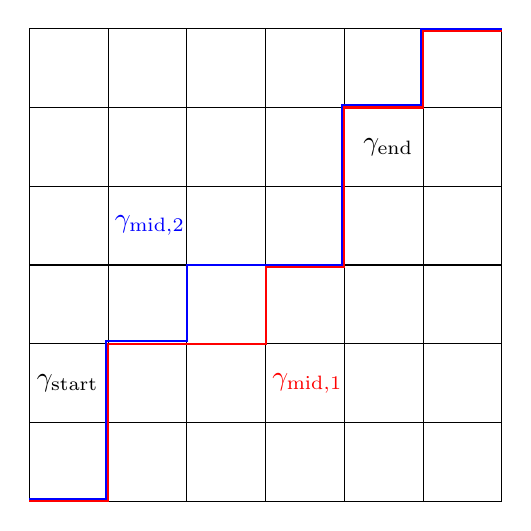
\begin{tikzpicture}
\draw (-3,3) -- (-3,-3);
\draw (-2,3) -- (-2,-3);
\draw (-1,3) -- (-1,-3);
\draw (0,3) -- (0,-3);
\draw (1,3) -- (1,-3);
\draw (2,3) -- (2,-3);
\draw(3,3) -- (3,-3);

\draw (-3,3) -- (3,3);
\draw (-3,2) -- (3,2);
\draw (-3,1) -- (3,1);
\draw (-3,0) -- (3,0);
\draw (-3,-1) -- (3,-1);
\draw (-3,-2) -- (3,-2);
\draw (-3,-3) -- (3,-3);

\draw[color=red,thick] (-3,-3) -- (-2,-3) -- (-2,-1) -- (0,-1) -- (0,-0.03) -- (1,-0.03) -- (1,2) -- (2,2) -- (2,2.97) -- (3,2.97);
\draw[color=blue,thick] (-3,-2.97) -- (-2.03,-2.97) -- (-2.03,-0.97) -- (-1,-0.97) -- (-1,0) -- (0.97,0) -- (0.97,2.03) -- (1.97,2.03) -- (1.97,3) -- (3,3);
\draw (-2,-1.5) node[left] {$\gamma_{\mathrm{start}}$};
\draw[color=red] (1.1,-1.5) node[left] {$\gamma_{\mathrm{mid,1}}$};
\draw[color=blue] (-0.9,0.5) node[left] {$\gamma_{\mathrm{mid,2}}$};
\draw (2,1.5) node[left] {$\gamma_{\mathrm{end}}$};

\end{tikzpicture}
$$




Then we can write $\gamma_i = \gamma_{\mathrm{start}} \star \gamma_{\mathrm{mid}, i} \star \gamma_{\mathrm{end}}$ for $i \in \{1,2\}$. Then we compute
\setlength{\abovedisplayskip}{5.5pt}
\setlength{\belowdisplayskip}{5.5pt}
\begin{alignat*}{5}
\F([\gamma_1]) \ &=&& \ \F([\gamma_{\mathrm{start}} \star \gamma_{\mathrm{mid}, 1} \star \gamma_{\mathrm{end}}]) \\
&=&& \ F_U([\gamma_{\mathrm{end}}]) \circ F_U([\gamma_{\mathrm{mid},1}]) \circ F_U([\gamma_{\mathrm{start}}]) \\
&=&& \ \ F_U([\gamma_{\mathrm{end}}]) \circ F_U([\gamma_{\mathrm{mid},2}]) \circ F_U([\gamma_{\mathrm{start}}]) \\
&=&& \ \F([\gamma_2]),
\end{alignat*}
where we used that $\gamma_{\mathrm{mid},1}$ and $\gamma_{\mathrm{mid},2}$ are homotopic relative endpoints. Using this, we can move the edge path through the lower right corner to the edge path through the upper left corner step by step through changes within one little square each time. But these edge paths differ from $\gamma$ and $\gamma'$ only by constant paths, i.e. we obtain 
$$\F([\gamma]) = \F([\gamma']).$$

\end{compactenum}
Now by construction $\F$ is a functor and factorizes the given cocone $(F_U: \Pi(U) \la G)_{U \in \mathcal{O}}$ over $(p_U: \Pi(U) \la \Pi(X))_{U \in \mathcal{O}}$. It remins to show that $\F$ is unique. Let $\F'$ be another morphism $\F': \Pi(X) \la G$ factorizing over $\Pi(U) \la \Pi(X)$. Then we have 
$$\F'([\gamma]) = \F'([\gamma_1 \star \ldots \star \gamma_n]) = F_{U_{i_n}}([\gamma_n]) \circ \ldots \circ F_{U_{i_1}}([\gamma_1]) = \F([\gamma])$$
when using a suitable refinement, which finishes the proof. $\hfill \Box$

\end{pr}










\section{Van Kampen's theorem in action} %PARAGRAPH II.3





For the most common application of van Kampen's theorem one decomposes $X= U_1 \cup U_2$ with open subsets $U_1, U_2$ such that $U_1 \cap U_2$ is path connected. Then by the groupversion of van Kampen's theorem, the pushout diagram
$$
\begin{xy}
\xymatrix{
U_1 \cap U_2 \ar[rr] \ar[d] && U_1 \ar[d] \\ U_2 \ar[rr] && X 
}
\end{xy}
$$
is preserved by the functor $\pi_1(\cdot, x_0)$ for some $x_0 \in U_1 \cap U_2$, i.e.
$$
\begin{xy}
\xymatrix{
\pi_1(U_1 \cap U_2, x_0) \ar[rr] \ar[d] && \pi_1(U_1, x_0) \ar[d] \\ \pi_1(U_2, x_0) \ar[rr] && \pi_1(X,x_0) }
\end{xy}
$$
is a pushout diagram. Then, by knowing $\pi_1(U_1, x_0)$, $\pi_1(U_2, x_0)$ and $\pi_1(U_1 \cap U_2,x_0)$ one can compute $\pi_1(X, x_0)$ by lemma I.5.21.

\begin{ex}
Let $X= \mathbb{S}^n$ for some $n \geqslant 2$ and let $U_1$ be a bit more than the upper hemisphere and respectively $U_2$ be a bit more than the lower one. Then $U_1, U_2$ are contractable, i.e. have trivial fundamental group. Then the corresponding pushout square reduces to
$$
\begin{xy}
\xymatrix{
\pi_1(U_1 \cap U_2, x_0) \ar[rr]^{\pi_1} \ar[d]^{\pi_2} && \{\id\} \ar[d] \\ \{\id\} \ar[rr] && \pi_1(X,x_0) }
\end{xy}
$$
Applying lemma I.5.21 we have 
$$\pi_1(X,x_0) = \slant{\{ \id\} \star \{ \id\} }{N}, \qquad N= \langle \pi_1(a) \pi_2^{-1}(a) \ \vert \ a \in \pi_1(U_1 \cap U_2, x_0) \rangle.$$
Thus, no matter what $\pi_1(U_1 \cap U_2, x_0)$ is we obtain $\pi_1(X, x_0) = \{\id\}$ and $X$ is simply connected.

\end{ex}



\begin{ex}
Let now $X= \mathbb{S}^1 \lor \mathbb{S}^1$ with basepoint $x_0$ and let $U_i:= X \setminus \{x_i\}$ with $x_1, x_2$ be in distinct circles and $x_i \neq x_0$ for $i \in \{1,2\}$. Then both $U_1$ and $U_2$ can be contracted to $\mathbb{S}^1$ and the corresponding fundamental groups are $\pi_1(U_i, x_0) = \pi_1(\mathbb{S}^1, x_0) \cong \mathbb{Z}$. More over, the intersection $U_1 \cap U_2$ can be contracted to a point, i.e. we have $\pi_1(U_1 \cap U_2, x_0) = \{ \id\}$. The pushput square then becomes to
$$
\begin{xy}
\xymatrix{
\{ \id\} \ar[rr] \ar[d] && \mathbb{Z} \ar[d] \\ \mathbb{Z} \ar[rr] && \pi_1(X,x_0)}
\end{xy}
$$
Applying Lemma I.5.21 with $N= \{ \id\}$ we obtain $\pi_1(X,x_0)= \mathbb{Z} \star \mathbb{Z} = F(a,b)$ the free group in two words.
For illustration of subgroups of the fundamental group, see Hatcher on page 58.



\end{ex}


\begin{ex}[Attaching cells]
Let $(X,x_0)$ be a pointed space and $f: (\mathbb{S}^{n-1}, \star) \la (X,x_0)$ be a a morphism of pointed spaces, i.e. $f(\star) = x_0$. Then we obtain a pushout diagram as in example I.5.20
$$
\begin{xy}
\xymatrix{
\mathbb{S}^{n-1} \ar[rr]^{f} \ar[d]_{i} && X \ar[d]^{\iota} \\ \mathbb{D}^n \ar[rr] && Y= X \cup_f \mathbb{D}^n}
\end{xy}$$

Set $y_0 := \iota(x_0)$. In order to compute $\pi_1(Y,y_0)$, we consider the two oben subsets
$$U_1= \mathrm{int}(\mathbb{D}^n) \subseteq Y, \qquad U_2 := X \cup_f (\mathbb{D}^n \setminus \{0\} ) \subseteq Y.$$
Then we have 
$$U_1 \cap U_2 = \mathbb{D}^n \setminus \{ \mathbb{S}^{n-1} \cup \{0\} \} \sim_{\mathrm{hom.}} \mathbb{S}^{n-1}.$$
Then we claim the following:

\begin{compactenum}
\item[(i)] If $n \geqslant 3$, then the morphism $\iota_* = \pi_1(\iota): \pi_1(X,x_0) \la \pi_1(Y,y_0)$ by the inclusion $\iota$ is an isomorphism.
\item[(ii)] If $n=2$, $\iota_*$ is surjective and $\ker \iota_*$ is the normal subgroup generated by $[f] \in \pi_1(X,x_0)$.
\end{compactenum}
We easily prove the statements:
\begin{compactenum}
\item Pick a basepoint $y_1 \in \mathrm{int}(\mathbb{D}^{n} \setminus \{0\})$ and a path
$$u: [0,1] \la \mathbb{D}^n \setminus \{0\}, \qquad u(0)=y_0, \ \ u(1) = y_1.$$
Since $U_1 \cap U_2$ is homotopy equivalent to $\mathbb{S}^{n-1}$ and $n \geqslant 3$, $U_1 \cap U_2$ is simply connected, i.e. $\pi_1(U_1 \cap U_2, y_1) = \{ \id\}$. Moreover $\pi_1(U_1, y_1) = \{ \id\}$. Then we use van Kampen's theorem to obtain a pushout diagram
$$
\begin{xy}
\xymatrix{
\{ \id\} \ar[rr] \ar[d] && \{ \id \} \ar[d] \\ \pi_1(U_2, y_1) \ar[rr] && \pi_1(Y,y_0)
}
\end{xy}
$$


Thus we have 
$$\pi_1(Y,y_0) \cong \pi_1(Y,y_1) \cong \slant{\{ \id\} \star \pi_1(U_2, y_1)}{N} \cong \pi_1(U_2, y_1).$$
Since we have a path from $y_0$ to $y_1$ entirely in $U_2$, the last one in the equation is isomorphic to $\pi_1(U_2, y_0)$. Further, we have a deformationretract between $U_2$ and $X$ (Since we missed out the centre of $\mathbb{D}^n$ in $U_2$, we can retract $\mathbb{D}^{n}\setminus \{0\}$ onto $f(\mathbb{S}^{n-1}) \subseteq X$), i.e. $U_2$ and $X$ have identical fundamental groups. Finally we obtain 
$$\pi_1(Y,y_0) \cong \pi_1(X,x_0).$$


\item Now let $n=2$. Then $U_1 \cap U_2$ is homotopy equivalent to $\mathbb{S}^1$, thus $\pi_1(U_1 \cap U_2, y_1) \cong \mathbb{Z}$. Our van-Kampen-pushout now looks like
$$
\begin{xy}
\xymatrix{
\mathbb{Z} \ar[rr] \ar[d]_{g} && \{ \id \} \ar[d] \\ \pi_1(U_2, y_1) \ar[rr] && \pi_1(Y,y_0) }
\end{xy}
$$
where $g$ is given by
$$g: \pi_1(U_1 \cap U_2, y_1) \cong \mathbb{Z} \la \pi_1(U_2, y_1), \qquad [\gamma] \mapsto [u^{-1} \star \gamma \star u^{-1}].$$
Again we can retract $U_2$ to $X$, thus $\pi_1(U_2, y_1) \cong \pi_1(X,x_0)$ and we have
$$\pi_1(Y,y_0) \cong \pi_1(Y,y_1) \cong \slant{\pi_1(X,x_0) \star \{ \id \}}{N} \cong \slant{\pi_1(X,x_0)}{N([f])}.$$



\end{compactenum}
\end{ex}


\begin{ex}
The torus $\mathbb{T}^2 = \slant{[0,1]^2 }{\sim}$ where opposite edges are identified in the same direction, is obtained from $\mathbb{S}^1 \lor \mathbb{S}^1$ by attaching a $2$-cell. Then
$$\pi_1(\mathbb{T}^2, x_0) = \langle a,b \ \vert \ aba^{-1}b^{-1} \rangle \cong \mathbb{Z} \oplus \mathbb{Z}.$$
Alternatively we have 
$$\pi_1(\mathbb{T}^2, x_0) = \pi_1( \mathbb{S}^1 \times \mathbb{S}^1) = \pi_1(\mathbb{S}^1) \times \pi_1(\mathbb{S}^1, x_0) = \mathbb{Z} \times \mathbb{Z} = \mathbb{Z}^2.$$
\end{ex}
\newpage
\begin{ex}
The oriented, closed, connected surfaces of genus $2$ are isomorphic to the torus with two holes. More generally the oriented closed connected surface of genus $g$ is given by
$$
\begin{xy}
\xymatrix{
\mathbb{S}^1 \ar[rr]^{\Pi [a_i, b_i]} \ar[d] && \bigvee_{i=1}^{2g} \mathbb{S}^1 \ar[d] \\ \mathbb{D}^2 \ar[rr] && F_{g}
}
\end{xy}
$$
and the $2g$ copies of $\mathbb{S}^1$ are labeled $a_1, b_1, \ldots, a_g, b_g$. Then 
$$\pi_1(F_g, x_0) \cong \langle a_1, b_1, \ldots, a_g, b_g \ \vert \ \Pi_{i=1}^g [a_i, b_i] \rangle.$$



\end{ex}




\begin{proposition}[presentation complex]
Le $G= \langle S \vert R \rangle$ be a finitely presented group. Then then there exists a twodimensional cell complex $(X,x_0)$ with $\pi_1(X,x_0) \cong G$.

\begin{pr}
Let $S= \{s_1, \ldots, s_n\}$ and $R= \{r_1, \ldots, r_m\}$ and set $Y_0 := \bigvee _{i=1}^n \mathbb{S}^1$ with some basepoint $y_0$. Orient and label the circles by $s_i$. Then we have $\pi_1(Y_0, y_0) \cong F(s_1, \ldots, s_n)$. The word $r_1$ defines an element $[\gamma_{r_1}]$ with some $\gamma_{r_1}: (\mathbb{S}^1, \star) \la (Y_0, y_0)$. Set $Y_1 := Y_0 \cup_{\gamma_{r_1}} \mathbb{D}^2$. Then by Example 3.3 we have 
$$\pi_1(Y_1, y_0) \cong \slant{\pi_1(Y_0, y_0)}{N([\gamma_{r_1}]}.$$
Now let $r_2 \in R$ be the next generator. Then $r_2$ defines an element $[\gamma_{r_2}]$ for some $\gamma_{r_2}: (\mathbb{S}^1, \star) \la (Y_0, y_0)$. Let $i_1: (Y_0,y_0) \la (Y_1, y_0)$ be the inclusion and further set $Y_2:= Y_1 \cup_{\gamma_{r_2}} \mathbb{D}^2$. Then 
\setlength{\abovedisplayskip}{5.5pt}
\setlength{\belowdisplayskip}{5.5pt}
\begin{alignat*}{5}
\pi_1(Y_2, y_0) \ \ &\cong&& \ \  \slant{\pi_1(Y_1, y_0)}{N([i_1 \circ \gamma_{r_2}]} \\
&\cong&& \ \ \slant{\pi_1(Y_1, y_0)}{N({i_1}_*([\gamma_{r_2}]))} \\
&\cong&& \ \ \slant{\pi_1(Y_1, y_0)}{N({i_1}_*([\gamma_{r_1}]), {i_1}_*([\gamma_{r_2}]))} \\
&\cong&& \ \ \slant{\pi_1(Y_1,y_0)}{{i_1}_*(N([\gamma_{r_1}], [\gamma_{r_2}]))} \\
&\cong && \ \ \bigslant{  \left( \slant{ \pi_1(Y_0, y_0)}{N([\gamma{r_1}])} \right)}{\left( \slant{N([\gamma_{r_1}], [\gamma_{r_2}])}{N([\gamma_{r_1}])} \right)} \\
&\cong&& \ \ \slant{\pi_1(Y_0,y_0)}{N([\gamma_{r_1}], [\gamma_{r_2}])}.\\
\end{alignat*}
Continuing this way we obtain
$$\pi_1(Y_m,y_0) \cong \slant{\pi_1(Y_0, y_0)}{N([\gamma_{r_1}], \ldots, [\gamma_{r_m}])} \cong \langle s_1, \ldots, s_r \vert r_1, \ldots, r_m \rangle  \cong G.$$
Thus we can choose $(X_0, x_0) = (Y_m, y_0)$. $\hfill \Box$

\end{pr}


\end{proposition}

\begin{remark}
Note that proposition 3.6 holds even if we drop the finite presentation of $G$.
\end{remark}









\section{On pushouts in Top} %PARAGRAPH II.4




\begin{definbem}
Let $X,Y$ be topological spaces, $f:X \la Y$ a map. Then the following statements are equivalent:
\begin{compactenum}
\item $f$ is an identification map.
\item $f$ is surjective and $U \subseteq Y$ is open iff $f^{-1}(U) \subseteq X$ is open.
\item $f$ is induces an homeomorphism $\tilde{F}: \slant{X}{\sim} \la Y$ where $x \sim y$ iff $f(x) = f(y)$.
\item Any map $g: Y \la W$ is continuous if and only if $g \circ f$ is continuous.
\end{compactenum}
\end{definbem}



\begin{theorem}
Let $A,X,Y,Z,k$ be topological spaces and assume $k$ to be locally compact.
\begin{compactenum}
\item If $X$ is compact, then the projection $p_Y: X \times Y \la Y$ is a closed map.
\item If $f: X \la Y$ is an identification map, so is $f \times \id_k: X \times k \la Y \times k$.
\item If
$$
\begin{xy}
\xymatrix{A \ar[rr]^{f_2} \ar[d]_{f_1} && Y \ar[d]^{g_2} \\ X \ar[rr]_{g_1} && Z
}
\end{xy}
$$ 
is a pushout square, so is
$$
\begin{xy}
\xymatrix{
A \times k \ar[rr]^{f_2 \times \id_k} \ar[d]_{f_1\times \id_k} && Y\times k \ar[d]^{g_2\times \id_k} \\ X\times k \ar[rr]_{g_1 \times \id_k} && Z \times k
}
\end{xy}
$$
\end{compactenum}

\begin{pr}

\begin{compactenum}
\item Let $C \subseteq X \times Y$ be closed. To show that $p_Y(C) \subseteq Y$ is closed is equivalent to showing that $Y \setminus P_Y(C)$ is open, i.e. that any $y \in Y \setminus p_Y(C)$ is an inner point. Now let $y \in Y\setminus p_Y(C)$. Then for all $x \in X$ we have that $(x,y) \notin C$, thus each $x \in X$ comes with open neighbourhoods $U_x \subseteq X$ of $x$ and $V_x \subseteq Y$ of $y$ such that $(U_x \times V_X) \cap C = \emptyset$. We obtain a cover $\{U_x\}_{x \in X}$ of $X$ and since $X$ is compact we can select finitely many $x_1, \ldots, x_n \in X$ such that $X= \bigcup_{k=1}^n U_{x_k}$. Set $V= \bigcup_{k=1}^n V_{x_k}$. Then $V$ is open with $y \in V$ and further we have $(X \times V) \cap C = \emptyset$, i.e. $V \subseteq Y\setminus p_Y(C)$. Thus $y$ is an inner point.

\item Let $f: X\la Y$ be an identification map. We will use characterization (iv) of definition 4.1 in order to show that $f \times \id_k$ is an identification map as well. Thus let $g: Y \times k \la W$ an arbitrary map of sets. We have to show that $f$ is continuous iff $h:= g \circ (f \times \id_k)$ is continuous. If $g$ is continuous, then for any open $U \subseteq W$ we have that $h^{-1}(U) = (g \circ (f \times \id_k))^{-1}(U) = f^{-1}(g^{-1}(U))$ is open in $X \times k$ since $g^{-1}(U)$ is open in $Y \times k$ (recall that $f$ is an identification map). Now let $h$ be continuous and $U \subseteq W$ any open set. We have to show, that $g^{-1}(U)$ is open in $Y \times k$, i.e. that all $(y_0, k_0) \in g^{-1}(U)$ are inner points. Let $(y_0, k_0) \in g^{-1}(U)$. Since $f$ is surjective, we can write $y_0 = f(x_0)$ for some $x_0 \in X$. Then $h(x_0, k_0) \in U$, i.e. $(x_0, k_0) \in g^{-1}(U)$. Since $k$ is locally compact, there exists a copact neighbourhood $N \subseteq k$ of $k_0$, such that
$h(\{x_0\} \times N) \subseteq U.$
Now set $$A:= \{ y\in Y \ \vert \ g(\{y\} \times N) \subseteq U \}.$$
Then $y_0 \in A$ and $A$ is open: We have that
$$f^{-1}(A)= \{ x \in X \ \vert \ h(\{x\} \times N) \subseteq U\},$$
thus if $p_X: X \times N \la X$ is the projection, we obtain
$$X \setminus f{-1}(A) = p_X(h^{-1}(W \setminus U) \cap (X \times N)).$$
Since $h$ is continuous, $h^{-1}(W \setminus U)$ is closed in $X \times k$, thus closed in $X \times N$ with the subspace topology. With part (i) we have that $X \setminus f^{-1}(A)$ as the projection is closed as well, i.e. $f^{-1}(A)$ and finally $A$ is open, which implies the assertion.
\item By assumption the coproduct map $g_1 \amalg g_2: X \amalg Y \la Z$ is an identification map (recall how the coproduct of spaces looked like). By part (ii) the map
$$h:=g_1 \times \id_k \amalg g_2 \times \id_k : (X \times k) \amalg (Y \times k) \la Z \times k$$
is an identifcation map as well and by 4.1 (iii) we obtain a homeomorphism
$$\overline{h}:=\overline{g_1 \times \id_k \amalg g_2 \times \id_k}: \slant{(X \times k) \amalg (Y \times k)}{\sim} \la Z \times k$$
where 
$(x,k) \sim (y,k')$ iff$ g_1(x) = g_2(y) \textrm{ and } k=k'$ where the first condition is equivalent to to the fact there exists $a \in A$ with $f_1(a)=x$ and $f_2(a)=y$. We obtain a diagram
$$
\begin{xy}
\xymatrix{
A \times k \ar[rr]^{f_2 \times \id_k} \ar[d]_{f_1 \times \id_k} && Y \times k \ar[d] \ar@/^{16pt}/[rrdd]^{g_2 \times \id_k} \\ X \times k \ar[rr] \ar@/_{16pt}/[rrrrd]_{g_1 \times \id_k} && \slant{X \times k \amalg Y \times k}{\sim} \ar[rrd]^{\overline{h}} && \\ &&&& Z \times k
}
\end{xy}
$$
and $\overline{h}$ is the uniqure arrow which fits into the diagram, thus it is a pushout square. $\hfill \Box$
\end{compactenum}
\end{pr}


\end{theorem}

\begin{theorem}   %%Theorem 2.4.3
Let 
$$
\begin{xy}
\xymatrix{
A \ar[rr]^{i_2} \ar[d]_{i_1} && Y \ar[d]^{j_1} \\ X \ar[rr]_{j_2} && Z
}
\end{xy}
$$
be a pushout square such that $i_1$ is the inclusion of a closed subspace as a neighbourhood deformation retract (NDR). Then so is $j_1$. 
\begin{pr}
First we note that $(j_2 \amalg j_1)^{-1} (j_1(Y)) = A \cup Y \subseteq X \amalg Y$ is closed, therefore $j_1(Y) \subseteq Z$ is closed since $j_2 \amalg j_1$ is an identification map. Next we sho, that $j_1: Y \la j_1(Y)$ is a homeomorphism. $j_1$ is injective, since $i_1$ is injective. Thus $j_1$ is a bijection on its image. We now have to show that the inverse map is continuous. Let thus $W \subseteq j_1(Y)$ be a subset such that $j_1^{-1}(W)$ is closed. Then $(j_2 \amalg j_1)^{-1}(W)$ is closed, thus $ W\subseteq Z$ is closed. Then $W \subseteq j_1(Y)$ is also closed.\\
Let now $A \subseteq U \subseteq X$ be an open neighbourhood of $A$ in $X$ such that $U$ (strongly) deformation retracts onto $A$, i.e. there is a retraction $r:U \la A$ and a homotopy $H: U \times I \la U$ with $H_0 = \id_U$, $H_1 = i_1 \circ r$ and $H_t \vert_A = \id_A$. Let $V= j_1(Y) \cup j_2(U)$. We show that $V\subseteq Z$ is open. We have
$$(j_2 \amalg j_1)^{-1}(V) = U \cup Y \overset{\mathrm{open}}{\subseteq} X \amalg Y$$
and by the propoerties of identification maps $V$ is open in $Z$. Moreover
$$
\begin{xy}
\xymatrix{
A \ar[rr]\ar[d]&& Y \ar[d] \\ U \ar[rr] && V } 
\end{xy}
$$
is a pushout square, thus also 

$$
\begin{xy}
\xymatrix{
 A\times I \ar[rr]^{i_2 \times \id_I} \ar[dd]_{i_1 \times \id_I} && Y \times I \ar[dd]^{j_1 \times \id_I} \ar@/^{16pt}/[rrddd]^{j_1 \circ \mathrm{pr}_Y} \\ &&& \\ U \times I \ar[rr]_{j_2 \times \id_I} \ar@/_{16pt}/[rrrrd]_{j_2 \circ H} && V \times I \ar@{-->}[rrd]_{\exists ! H'} && \\ &&&& V
}
\end{xy}
$$
is a pushout square, from which we will get the dsired homotopy $H'$. Note that the bent arrows define a cocone, which means that the outer part of the diagram commutes. Indeed
\begin{alignat*}{5}
(j_2 \circ H) \circ (i_1 \times \id_I)(a,t)\ & =&& \  j_2(h_t(i_1(a))) = (j_2 \circ i_1)(a) = (j_1 \circ i_2)(a) = (j_1 \circ \mathrm{pr}_Y)(i_2(a),t)\\
&=&& \ (j_1 \circ \mathrm{pr}_Y) \circ (i_2 \times \id_I)(a,t).
\end{alignat*}
Now set $r'=H_1'$. Then the upper triangle says that points in $j_1(Y) \subseteq V$ are fixed by $r'$ and the lower triangle says that points in $j_2(U)$ are retracted onto $(j_2 \circ i_1)(A) \subseteq V$. Thus $r'$ retracts $V$ onto $j_1(Y)$ and $\id_V \sim_{H'} r'$. The upper triangle says moreover that this homotopy is stationary on $j_1(Y)$, in other words $H'$ is a homotopy relative $j_1(Y)$, so $j_1(Y)$ is a strong deformation retract of $V$ under $H'$, which finishes the proof. $\hfill \Box$

\end{pr}
\end{theorem}


\begin{remark}
\begin{compactenum}
\item \textit{Subcomplexes} of \textit{CW-complexes} are exemples for closed neighbourhood deformation retracts (later in the course).
\item More generally, \textit{cofibrations} are preserved under pushouts (not in this course).
\end{compactenum}
\end{remark}







\section{One more Version of van Kampen's theorem} %PARAGRAPH II.5




\begin{theorem}[van Kampen's theorem - CNDR version]
Let 
$$
\begin{xy}
\xymatrix{
A \ar[rr]^{i_2} \ar[d]_{i_1} && Y \ar[d]_{j_1} \\ X \ar[rr]_{j_2} && Z
}
\end{xy}
$$
be a pushout square, such that $i_1, i_2$ are inclusions of closed NDRs. Assume $A,X,Y$ are path connected and $x_0 \in A$. Then applying $\pi_1$ gives us a pushout square in the category of groups.
\begin{pr}
Let $U_X \subseteq X$, $U_Y \subseteq Y$ be open neighbourhoods of $A$ which deformation retract onto $A$. Then applying the group version of van Kampen's theorem to 

$$
\begin{xy}
\xymatrix{
U_X \cup U_Y \ar[rr] \ar[d] && Y \cup U_X \ar[d] \\ X \cup U_Y \ar[rr] && Z
}
\end{xy}
$$
gives us the claim, since in the proof of the last theorem we have seen, that $U_X \cup U_Y$ is homotopy equivalent to $A$, $X \cup U_Y$ to $X$ and $Y \cup U_X$ to $Y$. $\hfill \Box$

\end{pr}

\end{theorem}


\begin{ex}
Let $X$ be the space obrtained from $\mathbb{S}^1 \times [0,1]$ by identifying
$$(z,0) \sim \left(e^{\frac{2\pi i}{n}}, 0\right), \qquad (z,1) \sim \left(e^{\frac{2\pi i}{m}}, 1\right).$$ Let $X_t$ be the upper part of the cylinder and $X_b$ the lower one respectively. Then we have a pushout

$$
\begin{xy}
\xymatrix{
\mathbb{S}^1 \ar[rr] \ar[d] && X_t \ar[d] \\ X_b \ar[rr] && X
}
\end{xy}
$$

Applying $\pi_1$ gives us
$$
\begin{xy}
\xymatrix{
\mathbb{Z} \ar[rr]^{x \mapsto x^m} \ar[d]_{x \mapsto x^n} && \mathbb{Z} \ar[d] \\ \mathbb{Z} \ar[rr] &&\pi_1(X)
}
\end{xy}
$$

Thus
$$\pi_1(X) = \langle a,b \ \vert \ a^mb^{-n} \rangle.$$
To see, that $\pi_1(X)$ is not trivial, consider the epimorphism
$$\pi_1(X) = \langle a,b \ \vert \ a^m b^{-m} \rangle \la \slant{\mathbb{Z}}{n \mathbb{Z}} \star \slant{\mathbb{Z}}{m \mathbb{Z}}, \qquad \begin{cases} \ a \mapsto [1]_{m} \\ \ b \mapsto [1]_n. \end{cases} $$

\end{ex}







\newpage
\thispagestyle{empty}























\chapter{Homology: Ideas and axioms} %KAPITEL III
\setlength\abovedisplayshortskip{0pt}
\setlength\belowdisplayshortskip{10pt}
\setlength\abovedisplayskip{10pt}
\setlength\belowdisplayskip{10pt}



\section{Motivation} %PARAGRAPH III.1

\thispagestyle{empty}


The fundamental group $\pi_1(X,x_0) = \slant{ \{ (\mathbb{S}^1, \star) \la (X,x_0) \}}{\sim}$ of a pointed space is defined on terms of low-dimensional data. Thus it is good at distiguishing low-dimensional spaces. For example, we can find out $\mathbb{S}^1 \ncong \mathbb{S}^2$ considering the fundamental groups $\{ \id\} = \pi_1(\mathbb{S}^2) \ncong \pi_1(\mathbb{S}^1) \cong \mathbb{Z}$. However, when distinguishing higher dimensional spaces, these information are not very useful. For example, we have $\pi_1(\mathbb{S}^m) \cong \pi_1(\mathbb{S}^n)$ for $m,n \in \mathbb{N}$, $m,n \geqslant 2$ although the spheress are non isomorphic unless $m=n$. Now there are various possible remedies.\\
Consider the higher homotopy groups $\pi_n(X,x_0) = \slant{\{ (\mathbb{S}^n, \star) \la (X,x_0)\}}{\sim}$. These are easy to define. However we have an insatisfactory result that $\pi_k(\mathbb{S}^n, \star) \cong \mathbb{Z}$ if $k=n$ and $\pi_k(\mathbb{S}^n, \star) \cong \{ \id\}$ if $k <n$. Even worse: The groups for $k>n$ are not known yet, since higher homotopy groups are very hard to compute.\\
Another possibility is the homology $H_k(X)$ of a space. It is very easy to compute and has the more satifying result 
$$H_k(\mathbb{S}^n)\ \  \cong \ \ \begin{cases} \ \mathbb{Z}, & \ \textrm{ if } k \in \{0,n\} \\
 \ \{ \id\}, & \ \textrm{ otherwise. }  \end{cases}$$
The hardest part will be to define homology. The idea is to proceed as follows:
\begin{compactenum}
\item Let 
$$\Delta^n := \left\{ (x_0, \ldots, x_n) \in \mathbb{R}^{n+1} \ \bigg\vert \ \sum_{i=1}^n x_i = 1, \ x_i \geqslant 0 \textrm{ for all } i \in \{0, \ldots, n \} \right\}$$
be an $n$\textit{-simplex}. For example, $\Delta^0$ is a point, $\Delta^1$ is a line, $\Delta^2$ is an equilateral triangle, $\Delta^3$ is a tetraeder and so on.
\item Now consider a space $X$ which is triangulated by such simplices. 
\item An $n$-chain are $n$-simplices next to each other, where the intersection of such $n$-simplices is a again a $k$-simplex for $k\leqslant n$.  An $n$-chain is called an $n$-\textit{cycle}, if it has no boundary.
\item The main idea will be, not to distinguish between two cycles, if their difference is the boundary of an $n+1$-chain (draw a picture!).
\item Then the $n$-th homology group of $X$ will be defined as
$$H_n(X) = \ \slant{\{n\textrm{-cycles }\}}{\{\textrm{ boundaries of }n+1 \textrm{-chains}\}}$$
\end{compactenum}





\section{Simplicial homology} %PARAGRAPH III.2



Let $n \in \mathbb{N}$ and $\{v_0, \ldots, v_n\} \subseteq \mathbb{R}^n$ be the standard basis. Then $\Delta^n$ defined as above is precisely the convex hull of this set, write $\Delta^n=[v_0, \ldots, v_n]$ and call the $v_i$ \textit{vertices of} $\Delta^n$. Deleting the $i$-th vertice of $\Delta^n$ we obtain the $i$-th \textit{face} of $\Delta^n$, write $[v_0, \ldots \hat{v}_i, \ldots, v_n]$. We have a unique homeomorphism $\Delta^{n-1} \cong [v_0, \ldots, \hat{v}_i, \ldots, v_n]$ when requiring that it preserves the order of vertices. The boundary and the interior of $\Delta^n$ is defined as 
$$\partial \Delta^n = \bigcup_{i=0}^n [v_0, \ldots, \hat{v}_i, \ldots, v_n], \qquad \overset{\circ \ \ }{\Delta ^n} = \Delta^{n} \setminus \partial \Delta{n}$$


%\begin{tikzpicture}
  %\draw (-1,0)coordinate[label=below:{$v_0$}](v_0)
    %--(1,0)coordinate[label=below:${v_1}$](v_1)
    %--(0,1.73)coordinate[label=above:${v_2}$](v_2)
    %--cycle;
%\end{tikzpicture}


\begin{defin}
A $\Delta$\textit{-complex} is a topological space $X$ together with a family of continuous maps $\{ \sigma_{\alpha}^n: \Delta^n \la X \}_{\alpha \in I_n}$ for each $n \geqslant 0$ with arbitrary index sets $I_n$, such that
\begin{compactenum}
\item For each $n \in \mathbb{N}$, $\alpha \in I_n$ we have that $\sigma_{\alpha}^n \vert_{\overset{\circ \ \ }{\Delta^n}}$ is injective.
\item Each $x \in X$ lies in $\mathrm{im}\left( \sigma_{\alpha}^n \vert_{\overset{\circ\ \ }{\Delta^n}} \right)$ for exactly one $\sigma_{\alpha}^n$.
\item Each restriction $\sigma_{\alpha}^n \vert_{[v_0, \ldots, \hat{v}_i, \ldots, v_n]}$ is equal to some $\sigma_{\beta}^{n-1}$.
\item A subset $A\subseteq X$ is open if and only if $\left(\sigma_{\alpha}^n\right)^{-1}(A) \subseteq \Delta^{n}$ is open.

\end{compactenum}
$\sigma_{\alpha}^n$ is called an $n$\textit{-simplex} of the $\Delta$-complex $X$.

\end{defin}

\begin{ex}
Let $X= \mathbb{T}^2$ the torus. Then $X$ has the structure of a $\Delta$-complex by

$$
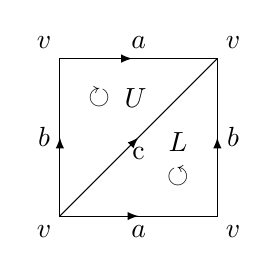
\begin{tikzpicture}
\draw[postaction={decorate},decoration={
    markings,
    mark=at position .125 with {\arrow{latex}},
    mark=at position .375 with {\arrow{latex}},
    mark=at position .635 with {\arrowreversed{latex}},
    mark=at position .875 with {\arrowreversed{latex}},
    }
  ]
    (0,0)  -- (2,0) node[midway, below] {$a$} --(2,2) node[midway, right] {$b$} --(0,2) node[midway, above] {$a$}  -- cycle node[midway, left] {$b$};
\draw[postaction={decorate},decoration={
    markings,
    mark=at position 0.5 with {\arrow{latex}}
    }
  ]
     (0,0) -- (2,2) node[midway, below] {c};
     
     
\draw (-0.2,0) node[below] {$v$};
\draw (2.2, 0) node[below] {$v$};
\draw (-0.2,2) node[above] {$v$};
\draw (2.2,2) node[above] {$v$};

\draw (0.5,1.5)  node {$\circlearrowright$};
\draw (1.5,0.5)  node {$\circlearrowleft$};

\draw (1.5,0.7) node[above] {$L$};
\draw (0.7,1.5) node[right] {$U$};

\end{tikzpicture}
$$
In order to determine the orientation of the $2$-simplices, consider the standard $2$-simplex, which is given by

$$
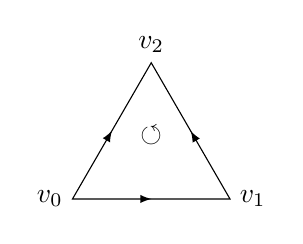
\begin{tikzpicture}

\draw[postaction={decorate}, decoration={markings,
mark=at position 0.167 with {\arrow{latex}},
mark=at position 0.5 with {\arrow{latex}},
mark=at position 0.833 with {\arrowreversed{latex}},
}
]
(0,0) -- (2,0) -- (1,1.73) -- cycle;

\draw (0,0) node [left] {$v_0$};
\draw (2,0) node[right] {$v_1$};
\draw (1,1.73) node[above] {$v_2$};
\draw (1,0.8) node {$\circlearrowleft$};
\end{tikzpicture}
$$

\end{ex}


\begin{ex}
Accordingly for the projective space $X= \mathbb{P}^2(\mathbb{R})$ we have a triangulization:

$$
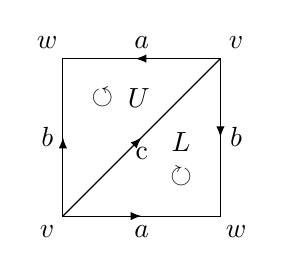
\begin{tikzpicture}
\draw[postaction={decorate},decoration={
    markings,
    mark=at position .125 with {\arrow{latex}},
    mark=at position .375 with {\arrowreversed{latex}},
    mark=at position .635 with {\arrow{latex}},
    mark=at position .875 with {\arrowreversed{latex}},
    }
  ]
    (0,0)  -- (2,0) node[midway, below] {$a$} --(2,2) node[midway, right] {$b$} --(0,2) node[midway, above] {$a$}  -- cycle node[midway, left] {$b$};
\draw[postaction={decorate},decoration={
    markings,
    mark=at position 0.5 with {\arrow{latex}}
    }
  ]
     (0,0) -- (2,2) node[midway, below] {c};
     
     
\draw (-0.2,0) node[below] {$v$};
\draw (2.2, 0) node[below] {$w$};
\draw (-0.2,2) node[above] {$w$};
\draw (2.2,2) node[above] {$v$};

\draw (0.5,1.5)  node {$\circlearrowleft$};
\draw (1.5,0.5)  node {$\circlearrowright$};

\draw (1.5,0.7) node[above] {$L$};
\draw (0.7,1.5) node[right] {$U$};
    

\end{tikzpicture}
$$


\end{ex}

\begin{ex} Analogously for the Klein Bottle we obtain

$$
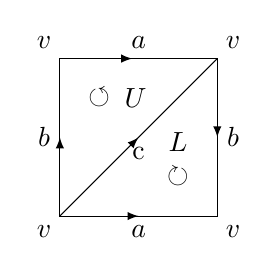
\begin{tikzpicture}
\draw[postaction={decorate},decoration={
    markings,
    mark=at position .125 with {\arrow{latex}},
    mark=at position .375 with {\arrowreversed{latex}},
    mark=at position .635 with {\arrowreversed{latex}},
    mark=at position .875 with {\arrowreversed{latex}},
    }
  ]
    (0,0)  -- (2,0) node[midway, below] {$a$} --(2,2) node[midway, right] {$b$} --(0,2) node[midway, above] {$a$}  -- cycle node[midway, left] {$b$};
\draw[postaction={decorate},decoration={
    markings,
    mark=at position 0.5 with {\arrow{latex}}
    }
  ]
     (0,0) -- (2,2) node[midway, below] {c};
     
     
\draw (-0.2,0) node[below] {$v$};
\draw (2.2, 0) node[below] {$v$};
\draw (-0.2,2) node[above] {$v$};
\draw (2.2,2) node[above] {$v$};

\draw (0.5,1.5)  node {$\circlearrowleft$};
\draw (1.5,0.5)  node {$\circlearrowright$};
    \draw (1.5,0.7) node[above] {$L$};
\draw (0.7,1.5) node[right] {$U$};

\end{tikzpicture}
$$


\end{ex}





\begin{defin}
A \textit{somplicial complex} is a $\Delta$-complex $X$ in which each simplex is uniquely determined by its vertices.
\end{defin}

\begin{remark}
The torus $\mathbb{T}^2$ as a simplicial complex need at least $14$ triangles, $21$ edges and $7$ vertices.
\end{remark}

\begin{defin}
Let $X$ be a $\Delta$-complex.
\begin{compactenum}
\item The $n$-th \textit{chain module} $C_n^{\Delta}(X)$ is the free $\mathbb{Z}$-module with basis $\{\sigma_{\alpha}^n: \Delta^n \la X\}_{\alpha \in I_n}$. Accordingly, an element
$$x=\sum_{\alpha \in I_n} k_{\alpha} \sigma_{\alpha}^n$$ in $C_n^{\Delta}(X)$ is called an $n$-\textit{chain} in $X$.
\item We have \textit{boundary homomorphisms} (or \textit{differentials}) between two neighboured chain modules given by
$$\partial_n: C_n^{\Delta}(X) \la C_{n-1}^{\Delta}(X), \qquad \sigma_{\alpha}^n \mapsto \sum_{i=0}^n (-1)^{i} \sigma_{\alpha}^n \vert_{[v_0, \ldots, \hat{v}_i, \ldots, v_n]}$$
We see, that the sign ensures coherent orientation. Consider for example the standard $2$-simplex:

$$
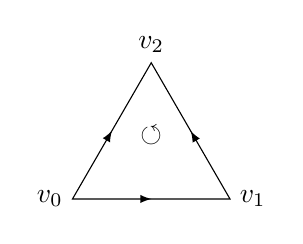
\begin{tikzpicture}

\draw[postaction={decorate}, decoration={markings,
mark=at position 0.167 with {\arrow{latex}},
mark=at position 0.5 with {\arrow{latex}},
mark=at position 0.833 with {\arrowreversed{latex}},
}
]
(0,0) -- (2,0) -- (1,1.73) -- cycle;

\draw (0,0) node [left] {$v_0$};
\draw (2,0) node[right] {$v_1$};
\draw (1,1.73) node[above] {$v_2$};
\draw (1,0.8) node {$\circlearrowleft$};
\end{tikzpicture}
$$
Reversing the arrow on the opposite of $v_1$ ($1$ is the only odd index) gives us a cycle of the three arrows.
\end{compactenum}
\end{defin}


\begin{defin}
Let $R$ be a ring and for $n \in \mathbb{Z}$ let $C_n$ be $R$-modules. Further let $d_n: C_n \la C_{n-1}$ be $R$-linear maps for all $n \in \mathbb{Z}$ such that $d_{n-1} \circ d_n = 0$ for all $n \in \mathbb{Z}$. Then the complex
$$(C_*, d_*)=\ldots \la C_{n+1} \overset{d_{n+1}}{\la} C_n \overset{d_n}{\la} C_{n-1} \la \ldots$$
is called a chain complex. Note that $d_{n+1} \circ d_n=0$ implies $\mathrm{im}\ d_{n+1} \subseteq \ker d_n$. We define the $n$-\textit{th homology modules} of $(C_*, d_*)$  to be $H_n(C_*) = \slant{\ker d_n}{\mathrm{im}\hspace{1pt} d_{n+1}}$.


\end{defin}

\begin{lemma}
Let $X$ be a $\Delta$-complex and $C_n^{\Delta}(X)$ and $\partial_n$ be as defined before. Then for all $n \in \mathbb{N}$ we have $\partial_{n-1} \circ \partial_n = 0$.
\begin{pr}
Let $\sigma := \sigma_{\alpha}^n \in C_n^{\Delta}(X)$. Then we have
\setlength{\abovedisplayskip}{5.5pt}
\setlength{\belowdisplayskip}{5.5pt}
\begin{alignat*}{5}
\partial_{n-1}\left(\partial_n(\sigma)\right) \ \ &=&& \ \ \partial_{n-1} \left( \sum_{i=0}^n (-1)^{i} \sigma \vert_{[v_0, \ldots, \hat{v}_i, \ldots, v_n]} \right) \\
&=&& \ \ \sum_{i=0}^n (-1)^{i} \partial_{n-1}\left( \sigma \vert_{[v_0, \ldots, \hat{v}_i, \ldots, v_n]} \right) \\
&=&& \ \ \sum_{i=0}^n (-1)^{i} \left( \sum_{j=0}^{i-1} (-1)^{j} \sigma \vert_{[v_0, \ldots, \hat{v}_j, \ldots, \hat{v}_i, \ldots, v_n]} + \sum_{j=i+1}^{n} (-1)^{j-1} \sigma \vert_{[v_0, \ldots, \hat{v}_i, \ldots, \hat{v}_j, \ldots, v_n]} \right) \\
&=&& \ \ \sum_{j<i} (-1)^{i} (-1)^{j} \sigma\vert_{[v_0, \ldots, \hat{v}_j, \ldots, \hat{v}_i, \dots, v_n]}  + \sum_{j>i} (-1)^{i} (-1)^{j-1} \sigma \vert_{[v_0, \ldots, \hat{v}_i, \ldots, \hat{v}_j, \ldots, v_n]} \\
&=&& \ \ \sum_{j<i} (-1)^{i} (-1)^{j} \sigma\vert_{[v_0, \ldots, \hat{v}_j, \ldots, \hat{v}_i, \dots, v_n]}  + \sum_{j<i} (-1)^{j} (-1)^{i-1} \sigma \vert_{[v_0, \ldots, \hat{v}_j, \ldots, \hat{v}_i, \ldots, v_n]} \\
&=&& \ \ \sum_{j<i} (-1)^{i-1} (1-1) (-1)^{j} \sigma\vert_{[v_0, \ldots, \hat{v}_j, \ldots, \hat{v}_i, \dots, v_n]}\\
&=&& \ \ 0,
\end{alignat*}
and since $\sigma$ was arbitrary, $\partial_{n-1} \circ \partial_n$ is equal to the zero map.$\hfill \Box$

\end{pr}

\end{lemma}


Thus
$$(C_*^{\Delta}(X), \partial_{*}) = \ldots \la C_{n+1}^{\Delta}(X) \overset{\partial_{n+1}}{\la} C_n^{\Delta} \overset{\partial_n}{\la} C_{n-1}^{\Delta} \la \ldots $$
is a \textit{chain complex} in the algebraic sense. If we interpret the kernel $\ker \partial_n$ as the set of $n$-cycles and $\mathrm{im} \hspace{1pt} \partial_{n+1}$ as the set of $n+1$-boundaries, we obtain, that the set of $n+1$-boundaries are contained in the set of $n$-cycles. In the rest of the course we will now and then use the notation
$$Z_n^{\Delta} =: Z_n := \ker \partial_n, \qquad B_n^{\Delta}:= B_n = \mathrm{im} \ \partial_{n+1}.$$
We now may define homology groups of our $\Delta$-complex to be
$$H_n^{\Delta}(X) := H_n(C_*^{\Delta}(X)).$$
$H_n^{\Delta}(X)$is called the $n$-\textit{th simplicial homology group} of the $\Delta$-complex $X$.
Now by definition of factor groups, two cycles $z_1, z_2 \in Z_n = \ker \partial_n$ represent the same element in $H_n^{\Delta}(X)$, if $z_1 - z_2 \in B_{n} =\mathrm{im} \partial_{n+1}$.



\begin{ex}
Let
$X= \mathbb{S}^1$ triangulated as follows:
$$
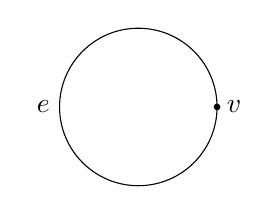
\begin{tikzpicture}
\draw (0,0) circle (1cm);
\node[mark size=1pt] at (1,0) {\pgfuseplotmark{*}};
\draw (1,0) node[right] {$v$};
\draw (-1,0) node[left] {$e$};
\end{tikzpicture}
$$
Then the chain complex looks like
$$\ldots \la  0 \la 0 \overset{\partial_2}{\la} \mathbb{Z} \cong \mathbb{Z} e= C_1^{\Delta}(\mathbb{S}^1) \overset{\partial_1}{\la} C_0^{\Delta}(\mathbb{S}^1) = \mathbb{Z} v \cong \mathbb{Z} \overset{\partial_0}{\la} 0 \la \ldots $$
where $\partial_1(e) = v-v = 0$. Thus $\partial_1$ is the zero map and we have
$$\ker \partial_1 = \mathbb{Z}, \qquad \mathrm{im} \hspace{1pt} \partial_2 = \{0\}, \qquad \ker \partial_0 = \mathbb{Z}, \qquad \mathrm{im} \hspace{1pt} \partial_1 = \{0\}$$
and we obtain 
$$H_k^{\Delta}(\mathbb{S}^1) = \begin{cases} \ \mathbb{Z}, & \ \textrm{ if } k \in \{0,1\} \\ \ \{0\}, & \ \textrm{ else. } \end{cases}$$



\end{ex}



\begin{ex}
Now consider the projective space $X= \mathbb{P}^2(\mathbb{R})$, triangulated as seen before:
$$
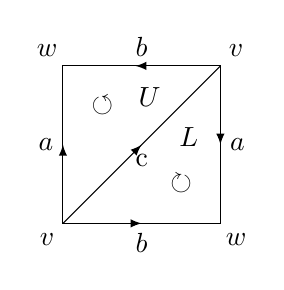
\begin{tikzpicture}
\draw[postaction={decorate},decoration={
    markings,
    mark=at position .125 with {\arrow{latex}},
    mark=at position .375 with {\arrowreversed{latex}},
    mark=at position .635 with {\arrow{latex}},
    mark=at position .875 with {\arrowreversed{latex}},
    }
  ]
    (0,0)  -- (2,0) node[midway, below] {$b$} --(2,2) node[midway, right] {$a$} --(0,2) node[midway, above] {$b$}  -- cycle node[midway, left] {$a$};
\draw[postaction={decorate},decoration={
    markings,
    mark=at position 0.5 with {\arrow{latex}}
    }
  ]
     (0,0) -- (2,2) node[midway, below] {c};
     
     
\draw (-0.2,0) node[below] {$v$};
\draw (2.2, 0) node[below] {$w$};
\draw (-0.2,2) node[above] {$w$};
\draw (2.2,2) node[above] {$v$};
\draw (1.1,1.6) node {$U$};
\draw (1.6,1.1) node {$L$};

\draw (0.5,1.5)  node {$\circlearrowleft$};
\draw (1.5,0.5)  node {$\circlearrowright$};
    

\end{tikzpicture}
$$

We have two $0$-simplices ($v$ and $w$), three $1$-simplices ($a$, $b$ and $c$) and two $2$-simplices ($L$ and $U$), thus 
$$C_0^{\Delta}(X) \cong \mathbb{Z} \oplus \mathbb{Z} \cong \mathbb{Z}^2, \qquad C_1^{\Delta}(X) \cong \mathbb{Z}^3, \qquad C_2^{\Delta}(X) \cong \mathbb{Z}^2.$$
and the others vanish.
Now let's investigate the boundary homomorphisms. We have
$$\partial_2(U) = -a + b + c, \qquad \partial_2(L) = a-b+c$$
$$\partial_1(a) = w-v, \qquad \partial_1(b) = w-v, \qquad \partial_1(c) = v-v = 0$$
and $\partial_0$ is the zero map as usual. Thus our chain complex is given by
$$\ldots \overset{\partial_4}{\la} 0 \overset{\partial_3}{\la} \mathbb{Z}^2 \overset{\partial_2}{\la} \mathbb{Z}^3 \overset{\partial_1}{\la} \mathbb{Z}^2 \overset{\partial_0}{\la} 0 \la \ldots$$
with 
$$\partial_2\left(z \right) = \begin{pmatrix}[rr]-1 & 1 \\[-6pt] 1 & -1 \\[-6pt] 1 & 1 \end{pmatrix} \cdot z = D_2 \hspace{1pt} z, \qquad \partial_1\left( z \right) = \begin{pmatrix}[rrr] -1 & -1 & 0 \\[-6pt] 1 & 1 & 0 \end{pmatrix} \cdot z = D_1 \hspace{1pt} z$$
Since $D_2$ has full rank, $\partial_2$ is injective, thus $\ker \partial_2= \{0\}$ and we have $H_2^{\Delta}(X) \cong \{0\}$. For the kernel of $\partial_1$ we have
$$\ker \partial_1 = \left\{ \begin{pmatrix}[r] k \\[-6pt]-k \\[-6pt] m \end{pmatrix}\  \bigg\vert \ k,m \in \mathbb{Z}\right\} = \left\{ k \hspace{1pt} \begin{pmatrix}[r]1\\[-6pt]-1\\[-6pt] 1\end{pmatrix} + k' \begin{pmatrix}0\\[-6pt]0\\[-6pt] 1\end{pmatrix} \ \bigg\vert\ k,k' \in \mathbb{Z} \right\},$$
where we write $m=k+k'$. For the image of $\partial_2$ we obtain by setting $p:= -r+s$, $r+s=p+2r=p+2q$
$$\mathrm{im} \hspace{1pt} \partial_2 = \left\{ \begin{pmatrix}[r] -r +s\\[-6pt] r-2 \\[-6pt] r+s\end{pmatrix} \ \bigg\vert \ r,s \in \mathbb{Z} \right\} = \left\{ p \begin{pmatrix}[r]1\\[-6pt]-1\\[-6pt]1\end{pmatrix} + 2q \begin{pmatrix}[r]0\\[-6pt]0\\[-6pt] 1\end{pmatrix} \ \bigg\vert \ p,q \in \mathbb{Z} \right\},$$
thus for the first homology group we have
$$H_1^{\Delta}(X) = \slant{\ker \partial_0}{\mathrm{im} \hspace{1pt}\partial_2} = \left\{ \begin{pmatrix}[r]0\\[-6pt]0\\[-6pt]0\end{pmatrix}, \begin{pmatrix}0\\[-6pt]0\\[-6pt]1\end{pmatrix} \right\} \cong \slant{\mathbb{Z}}{2\mathbb{Z}}.$$
Finally, since $\ker \partial_0=\mathbb{Z}^2$ and $\im\ \partial_1 \cong \Z$
%$$\mathrm{im}\hspace{1pt} \partial_1 = \left\{ \begin{pmatrix}[r]k\\[-6pt]-k\end{pmatrix} \ \big\vert \ k \in \mathbb{Z} \right\} \cong \mathbb{Z}$$
we have
$$H_0^{\Delta}(X) \cong \slant{\mathbb{Z}^2}{\mathbb{Z}} \cong \mathbb{Z}.$$



\end{ex}








\section{Relative simplicial homology with coefficients} %PARAGRAPH III.3





Let $X$ be a $\delta$-complex. A \textit{sub}-$\Delta$-\textit{complex} (or simply a \textit{subcomplex}) of $X$ is a subspace $A\subseteq X$given by a union of simplices of $X$. Observe that by definition, $A$ is closed. Indeed, we have that 
$$(\sigma_{\alpha}^n)^{-1}(A) = \bigcup \ \{ \textrm{subsimplices of } \Delta^n \}$$
and property (iv) of definition 2.1 implies that $A$ is closed. A $\Delta$\textit{-pair} is a pair $(X,A)$ consisting of a $\Delta$-complex $X$ and a sub-$\Delta$-complex $A$ of $X$.


\begin{ex}
Let $X$ be the standard $2$-simplex:
$$ 
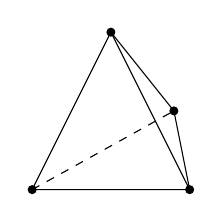
\begin{tikzpicture}
\draw[fill=black] (0.05,0) arc(0:360:0.05cm);
\draw[fill=black] (2.05,0) arc(0:360:0.05cm);
\draw[fill=black] (1.05,2) arc(0:360:0.05cm);
\draw (0,0) -- (2,0) -- (1,2) -- (0,0);
\draw[fill=black] (1.85,1) arc (0:360:0.05cm);
\draw (2,0) -- (1.8,1) -- (1,2);
\draw[dashed] (0,0) -- (1.8,1);
\end{tikzpicture}
$$
Then the subspace $A$ given by
$$ 
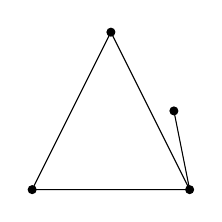
\begin{tikzpicture}
\draw[fill=black] (0.05,0) arc(0:360:0.05cm);
\draw[fill=black] (2.05,0) arc(0:360:0.05cm);
\draw[fill=black] (1.05,2) arc(0:360:0.05cm);
\draw (0,0) -- (2,0) -- (1,2) -- (0,0);
\draw[fill=black] (1.85,1) arc (0:360:0.05cm);
\draw (2,0) -- (1.8,1);
\end{tikzpicture}
$$
is a sub-$\Delta$-complex, where as $B$ given by 
$$
\begin{tikzpicture}
\draw[fill=black] (0.05,0) arc(0:360:0.05cm);
\draw[fill=black] (2.05,0) arc(0:360:0.05cm);
\draw[] (1.05,2) arc(0:360:0.05cm);
\draw (0,0) --(1,2);
\end{tikzpicture}
$$
is none.


\end{ex}


\begin{defin}
Let $(X,A)$ be a $\Delta$-pair. Then the $n$\textit{-th relative simplicial chain module} of $(X,A)$ is
$$C_n^{\Delta}(X,A) := \slant{C_n^{\Delta}(X)}{C_n^{\Delta}(A)},$$
i.e. chains in $A$ are identified with the trivial chain. For the boundary maps note that 
$$\partial_n(C_n^{\Delta}(A)) \subseteq C_{n-1}^{\Delta}(A)$$
Thus $\partial_n$ factorizes over $\slant{C_n^{\Delta}(X)}{C_n^{\Delta}(A)}$ and we get boundary maps of the relative chain modules
$$\partial_n: C_n^{\Delta}(X,A) \la C_{n-1}^{\Delta}(X,A).$$
Clearly, we still have $\partial_{n-1} \circ \partial_n=0$ and we can define the $n$\textit{-th relative simplicial homology} of $(X,A)$ to be 
$$H_n^{\Delta}(X,A) := H_n(C_*^{\Delta}(X,A)).$$

\end{defin}


\begin{ex}
Let $X= \Delta^n$ and $A= \partial \Delta^n$. Then $(X,A)$ is a $\Delta$-pair with chain modules
$$C_k^{\Delta}(X,A)\ \cong  \ \ \begin{cases} \ \mathbb{Z}, & \textrm{ if } k=n\\ \ \{0\}, & \textrm{ else,} \end{cases}$$
thus for the relative homology we obtain 
$$H_k^{\Delta}(X,A)\ \cong \ \ \begin{cases} \ \mathbb{Z}, & \textrm{ if } k=n\\ \ \{0\}, & \textrm{ else.} \end{cases}$$

\end{ex}



$\quad$ More generally let $X$ be a $\Delta$-complex, $R$ be a commutative ring with unity and let $C_n^{\Delta}(X;R)$ be the free $R$-module with basis $\{ \sigma_{\alpha}^n: \Delta^n \la X\}$. Then by the same construction as above we obtain the $n$\textit{-th relative simplicial chain module with coefficients in} $R$ of $(X,A)$
$$C_n^{\Delta}(X,A;R) := \slant{C_n^{\Delta}(X;R)}{C_n^{\Delta}(A;R)}$$
and the $n$\textit{-th relative simplicial homology with coefficients in} $R$
$$H_n^{\Delta}(X,A;R) := H_n^{\Delta}(X,A;R).$$

\begin{ex}
Recall example III.2.11, where we found the boundary map
$$\partial_2: \mathbb{Z}^2 = C_2^{\Delta}(\mathbb{P}^2(\mathbb{R}); \mathbb{Z}) \la C_1^{\Delta}(\mathbb{P}^2(\mathbb{R}); \mathbb{Z}) = \mathbb{Z}^3, \qquad z \mapsto \begin{pmatrix}[rr] -1 & 1 \\[-6pt] 1 & -1 \\[-6pt] 1 & 1 \end{pmatrix} \ z$$
Now let $R=\slant{\mathbb{Z}}{2 \mathbb{Z}}$. Then $\partial_2$ becomes
$$\partial_2: \left(\slant{\mathbb{Z}}{2 \mathbb{Z}}\right)^2 = C_2^{\Delta}(\mathbb{P}^2(\mathbb{R}); \mathbb{Z}) \la C_1^{\Delta}(\mathbb{P}^2(\mathbb{R}); \mathbb{Z}) = \left(\slant{\mathbb{Z}}{2 \mathbb{Z}}\right)^3, \qquad z \mapsto \begin{pmatrix}[rr] 1 & 1 \\[-6pt] 1 & 1 \\[-6pt] 1 & 1 \end{pmatrix} \ z$$
and is now a rank-$1$-linear map of $\left(\slant{\mathbb{Z}}{2 \mathbb{Z}}\right)$-vector spaces. In particular, we have
$$H_2^{\Delta}\left(\mathbb{P}^2(\mathbb{R}); \slant{\mathbb{Z}}{2 \mathbb{Z}} \right) \cong \slant{\mathbb{Z}}{2 \mathbb{Z}}.$$
\end{ex}


$\quad$ The relative homology $H_n^{\Delta}(X,A;R)$ measures the "difference" between $H_n^{\Delta}(X;R)$ and $H_n^{\Delta}(A;R)$. To make this precise, we introduce some algebraic terminology.


\begin{defin}
A sequence $A \overset{f}{\la} B \overset{g}{\la} C$ in $\Rmod$ is called \textit{exact at} $B$, if $\ker g = \mathrm{im} \hspace{1pt} f$. Observe that in this case $g$ is injective if and only if $f=0$ and $f$ is surjective if and only if $g=0$. A \textit{long exact sequence} in $\Rmod$ is a sequence
$$\ldots \la A_{n+1} \la A_n \la A_{n-1} \la A_{n-2} \la \ldots$$
which is exact everywhere.


\end{defin}


\begin{theorem}[long exact sequence]
Let $(X,A)$ be a $\Delta$-pair. Then we have a long exact sequence
$$\ldots \la H_n^{\Delta}(A;R) \overset{i_n}{\la} H_n^{\Delta}(X;R) \overset{j_n}{\la} H_n^{\Delta}(X,A;R) \overset{d_n}{\la} H_{n-1}^{\Delta}(A;R) \overset{i_{n-1}}{\la} H_{n-1}^{\Delta}(X;R) \la \ldots$$
%where $i_n$ is induced by $Z_n^{\Delta}(A;R) \la Z_n^{\Delta}(X;R)$, $j_n$ is induced by $Z_n^{\Delta}(X;R) \la Z_n^{\Delta}(X,A;R)$ and $d_n$ is induced by $\partial_n: Z_n^{\Delta}(X,A;R) \la Z_{n-1}^{\Delta}(A;R)$ and we use the standard notation 
%$$Z_n^{\Delta}(X,A;R) := \ker \left( \partial_n: C_n^{\Delta}(X,A;R) \la C_{n-1}^{\Delta}(X,A;R) \right), \qquad B_n^{\Delta}(X,A;R) := \mathrm{im} \hspace{1pt} \partial_{n+1}.$$

\begin{pr}
As an example we first construct the maps $i_n$. Consider the commutative ladder
$$
\begin{xy}
\xymatrix{
\ldots \ar[r] & C_{n+1}^{\Delta}(A;R) \ar[d]_{\iota_{n+1}} \ar[r]^{\partial^{A}_{n+1}} & C_n^{\Delta}(A;R) \ar[d]_{\iota_n} \ar[r]^{\partial^{A}_n} & C_{n-1}^{\Delta}(A;R) \ar[d]_{\iota_{n-1}} \ar[r] & \ldots \\
\ldots \ar[r] & C_{n+1}^{\Delta}(X;R) \ar[r]^{\partial^X_{n+1}} & C_n^{\Delta}(X;R) \ar[r]^{\partial^X_n} & C_{n+1}^{\Delta}(X;R) \ar[r] & \ldots
}
\end{xy}
$$
Then for $\sigma_{\alpha}^n \in \ker \partial_n^{A}$ we have 
$$0=\iota_{n-1}(0)=\iota_{n-1}\left(\partial^{A}_n(\sigma_{\alpha}^n)\right)= \partial^X_n\left( \iota_n(\sigma_{\alpha}^n)\right),$$
i.e. $\iota_n\left( \ker \partial^{A}_n\right) \subseteq \ker \partial^X_n$. Thus $\iota_n$ induces a homomorphism
$$\overline{\iota}_n: \ker \partial^{A}_n \la \slant{\ker \partial^X_n}{\mathrm{im} \ \partial^X_{n+1}} = H_{n}^{\Delta}(X;R).$$
Moreover for $\sigma_{\alpha}^n = \partial^{A}_{n+1}(\sigma_{\beta}^{n+1}) \in \mathrm{im} \ \partial^{A}_{n+1}$ we have
$$\overline{\iota}_n\left( \sigma_{\alpha}^n\right) = \left( \overline{\iota}_n \circ \partial^{A}_{n+1}\right)\left( \sigma_{\beta}^{n+1}\right) = \left( \partial^X_{n+1} \circ \iota_{n+1}\right)\left( \sigma_{\beta}^{n+1}\right) = \partial^X_{n+1} \left( \iota_{n+1}(\sigma_{\beta}^{n+1})\right) \in \mathrm{im} \ \partial^X_{n+1},$$
hence $\overline{\iota}_n$ uniquely factorizes over $\slant{\ker \partial^{A}_n}{\mathrm{im} \ \partial^{A}_{n+1}}= H_n^{\Delta}(A;R)$ and induces $i_n$. In the same way we can obtain $j_n$. 
For the boundary homomorphisms $d_n$ consider the chain complex of short exact sequences
$$
\begin{xy}
\xymatrix{
& 0 \ar[d] &0 \ar[d] & 0 \ar[d] & \\
\ldots \ar[r] & C_{n+1}^{\Delta}(A;R) \ar[dd]_{\iota_{n+1}} \ar[r]^{\partial^{A}_{n+1}} & C_n^{\Delta}(A;R) \ar[dd]_{\iota_n} \ar[r]^{\partial^{A}_n} & C_{n-1}^{\Delta}(A;R) \ar[dd]_{\iota_{n-1}} \ar[r] & \ldots \\ &&&&\\
\ldots \ar[r] & C_{n+1}^{\Delta}(X;R) \ar[dd]_{\pi_{n+1}} \ar[r]^{\partial^X_{n+1}} & C_n^{\Delta}(X;R) \ar[dd]_{\pi_n} \ar[r]^{\partial^X_n} & C_{n+1}^{\Delta}(X;R) \ar[dd]_{\pi_{n-1}} \ar[r] & \ldots \\ &&&& \\
\ldots \ar[r] & C_{n+1}^{\Delta}(X,A;R) \ar[d] \ar[r]^{\overline{\partial}^{X}_{n+1}} & C_n^{\Delta}(X,A;R) \ar[d] \ar[r]^{\overline{\partial}^{X}_{n}} & C_{n-1}^{\Delta}(X,A;R) \ar[d] \ar[r] & \ldots \\
& 0 & 0 & 0 & 
}
\end{xy}
$$
We want to construct
$$d_n: \slant{\ker \overline{\partial}_n^X}{ \mathrm{im} \ \overline{\partial}^X_{n+1}} = H_{n}^{\Delta}(X,A;R) \la H_{n-1}^{\Delta}(A;R) = \slant{\ker \partial_{n-1}^{A}}{\mathrm{im} \ \partial_n^{A}}.$$
Let $\sigma_{\alpha}^n \in \ker \overline{\partial}_n^X$ and consider a preimage $\tilde{\sigma}_{\alpha}^n \in C_n^{\Delta}(X;R)$. Then 
$$0=\overline{\partial}_n^X(\sigma_{\alpha}^n) = \left( \overline{\partial}_n^X \circ \pi_n\right) \left( \tilde{\sigma}_{\alpha}^n \right) = \left( \pi_{n-1} \circ \partial_n^X\right) \left( \tilde{\sigma}_{\alpha}^X\right),$$
i.e. $\partial_n^X(\tilde{\sigma}_{\alpha}^X) \in \ker \pi_{n-1} = \mathrm{im} \ \iota_{n-1}$, write $\partial_n^X(\tilde{\sigma}_{\alpha}^n) = \iota_{n-1}(\tilde{\sigma}_{\alpha}^{n-1})$ with some unique $\tilde{\sigma}_{\alpha}^{n-1}$ since $\iota_{n-1}$ is injective. Now define
$$\tilde{d}_n: \ker \overline{\partial}_n^X \la H_{n-1}^{\Delta}(A;R), \qquad \sigma_{\alpha}^n \mapsto \tilde{\sigma}_{\alpha}^{n-1}.$$
We have to show that this is well defined, i.e independant of the choice of the preimage $\tilde{\sigma}_{\alpha}^n$ of $\sigma_{\alpha}^n$ under $\pi_n$. Let $\sigma_{\beta}^n$ another simplex satisfying $\pi_n(\sigma_{\beta}^n)=\sigma_{\alpha}^n$ and write $\partial_n^X(\sigma_{\beta}^n) = \iota_{n-1}(\sigma_{\beta}^{n-1})$. Then
$$0= \sigma_{\alpha}^n- \sigma_{\alpha}^n =\pi_n(\sigma_{\beta}^n) - \pi_n(\tilde{\sigma}_{\alpha}^n) =  \pi_n(\sigma_{\beta}^n - \tilde{\sigma}_{\alpha}^n),$$
i.e. $\sigma_{\beta}^n - \tilde{\sigma}_{\alpha}^n \in \ker \pi_n = \mathrm{im} \ \iota_n$, write $\iota_n(\sigma_{\gamma}^n) = \sigma_{\beta}^n - \tilde{\sigma}_{\alpha}^n$. Then
$$\sigma_{\beta}^{n-1} - \tilde{\sigma}_{\alpha}^{n-1} = \iota_{n-1}^{-1}\left(\partial_n^X(\sigma_{\beta}^{n}- \tilde{\sigma}_{\alpha}^n)\right) =\partial_n^{A} \left( i_n^{-1}(\sigma_{\beta}^n - \tilde{\sigma}_{\alpha}^n) \right) = \partial_n^{A} \left( \sigma_{\gamma}^n\right) \in \mathrm{im} \ \partial_n^{A},$$
 which vanishes in $H_{n-1}^{\Delta}(A;R)$. Thus $\tilde{d}_n$ is well defined. It remains to show that $\tilde{d}_n$ factorizes over $H_n^{\Delta}(X,A;R)$. Let $\sigma_{\alpha}^n = \overline{\partial}^X_{n+1}(\sigma_{\alpha}^{n+1}) \in \mathrm{im} \ \overline{\partial}^X_{n+1} \subseteq \ker \overline{\partial}_n^X$ and choose preimages $\tilde{\sigma}_{\alpha}^{n+1} \in C_{n+1}^{\Delta}(X;A)$ of $\sigma_{\alpha}^{n+1}$ under $\pi_{n+1}$ and $\tilde{\sigma}_{\alpha}^n \in C_n^{\Delta}(X;R)$ under $\pi_n$. Then 
$$\partial_n^X\left( \tilde{\sigma}_{\alpha}^n\right) = \pi_{n-1}^{-1}\left( \overline{\partial}_n^X(\sigma_{\alpha}^n)\right) = \pi_{n-1}^{-1} \left( \overline{\partial}_n^X \circ \overline{\partial}_{n+1}^X \right)(\sigma_{\alpha}^{n+1}) = 0,$$
and thus $\tilde{d}_n(\sigma_{\alpha}^n)= \iota_{n-1}^{-1}(0)=0$ which shows $\mathrm{im} \ \overline{\partial}_n^X \subseteq \ker \tilde{d}_n$.\\
We now show $\ker i_n = \mathrm{im} \hspace{1pt} d_{n+1}$; exactness at the other modules works similar. But the preceeding follows immediately: $z+ B_n^{\Delta}(A;R)$ is in the kernel $\ker i_n$ if and only if $z \in B_n^{\Delta}(X;R) = \mathrm{im} \hspace{1pt} \partial_{n+1}$. But since $\partial_{n+1}$ is induced by $d_{n+1}$, we have $z + B_n^{\Delta}(A;R) \in \mathrm{im} \hspace{1pt} d_{n+1}$. $\hfill \Box$

\end{pr}
\end{theorem}

\begin{corollary}
Let $(X,A)$ be a $\Delta$-pair and $R$ be a ring. Then $H_n^{\Delta}(X,A;R)$ vanishes for all $n \in \mathbb{Z}$ if and only if for all $n$ the homomorphisms $i_n:H_n^{\Delta}(A;R) \overset{\sim}{\la} H_n^{\Delta}(X;R)$ in the long exact sequence of $(X,A)$ are isomorphisms.
\end{corollary}


$\quad$ To compute relative homology it is useful to know that on can excise subcomplexes:


\begin{theorem}[excision]
Let $X$ be a $\Delta$-complex, $A,Y \subseteq X$ be sub-$\Delta$-complexes of $X$ such that $\overline{A} \subseteq \mathrm{int} \hspace{1pt} Y := \overset{\circ}{Y}$. Then the inclusion of $\Delta$-pairs
$$j:\left( \overline{X \setminus A}, \overline{Y \setminus A} \right) \overset{j}{\hookrightarrow} (X,Y)$$
induces isomorphisms
$$H_n^{\Delta}\left( \overline{X \setminus A}, \overline{Y \setminus A};R\right) \overset{\sim}{\la} H_n^{\Delta}(X,Y;R)$$
for all $n \in \mathbb{Z}$.

\begin{pr}
We show more, namely that $C_n^{\Delta}(\overline{X\setminus A}, \overline{Y \setminus A}; R) \overset{j_n}{\cong} C_n^{\Delta}(X,Y;R)$ with $j_n:=C_n(j)$. For surjectivity of $j_n$ let $c+ C_n^{\Delta}(Y;R)$ be arbitrary in $C_n^{\Delta}(X,Y;R)$. Then we can find a representant $c' + C_n^{\Delta}(Y;R)$ where $c'$ has no nonzero coefficients on simplices in $Y$ (push them into $C_n^{\Delta}(Y;R)$). Since $X \setminus Y \subseteq X\setminus A \subseteq \overline{X \setminus A}$, the element $c' + C_n^{\Delta}(\overline{Y \setminus A};R)$ is a preimage of $c+ C_n^{\Delta}(Y;R)$ in $C_n^{\Delta}(\overline{X \setminus A}, \overline{Y \setminus A};R)$ under $j_n$. For injectivity let $c+ C_n^{\Delta}(\overline{X \setminus A}, \overline{Y \setminus A};R) \in \ker j_n$, i.e. $j_n\left(c+ C_n^{\Delta}(\overline{X \setminus A}, \overline{Y \setminus A};R)\right) = 0$. Then $c \in C_n^{\Delta}(\overline{X\setminus A} \cap Y;R)$. But since $A \subseteq \overset{\circ}{Y}$, we have $\overline{X \setminus A} \cap Y \subseteq \overline{Y \setminus A}$ and thus $c+C_n^{\Delta}(\overline{X \setminus A}, \overline{Y \setminus A};R) =0$ since $c \in C_n^{\Delta}(\overline{Y\setminus A};R)$. $\hfill \Box$




\end{pr}
\end{theorem}


\begin{remark}
Do we have $H_n^{\Delta}(A;R) \subseteq H_n^{\Delta}(X;R)$ and $H_h^{\Delta}(X,A;R) \cong \slant{H_n^{\Delta}(X;R)}{H_n^{\Delta}(A;R)}$? Answer: sometimes. Consider the long exact sequence
$$\overset{\partial_{n+1}}{\la} H_n^{\Delta}(A;R) \la H_n^{\Delta}(X;R) \la H_n^{\Delta}(X,A;R) \overset{\partial_n}{\la} H_{n-1}^{\Delta}(A;R) \la \ldots$$
Then the above holds if and only if $\partial_{n+1}=0 = \partial_n$. This happens for example. if $X$ retracts onto $A$ (see Problem 7.3).


\end{remark}


\begin{remark}[drawback of simplicial homology] 
To resume the results of the paragraph:
\begin{compactenum}
\item Simplicial homology is only defined for $\Delta$-complexes.
\item Morphisms between $\Delta$-complexes must be defines rigidly to turn $H_n^{\Delta}(-,-;R)$ into a functor $\underline{\Delta-\mathrm{pairs}} \la \Rmod$.
\item Then it is not clear, if $X \cong Y$ implies $H_n^{\Delta}(X;R) \cong H_n^{\Delta}(Y;R)$ let alone if $X \sim Y$ implies $H_n^{\Delta}(X;R) \cong H_n^{\Delta}(Y;R)$.
\item Ideally we want homology to be a family of functors $\toptwo \la \Rmod$, such that we have
\begin{compactenum}
\item a factorzation through $\hotoptwo$, i.e. we get a commutative diagram of functors
$$
\begin{xy}
\xymatrix{
& \hotoptwo \ar[rd] & \\ \toptwo \ar[ru] \ar[rr]_{H_n(-;R)} && \Rmod 
}
\end{xy}
$$
\item a long exact sequence for every pair $(X,A)\in \toptwo$
\item an excision isomorphism for certain triples $(X,Y,A)$.
\end{compactenum}
\end{compactenum}
\end{remark}














\section{The Eilenberg-Steenrod axioms for homology} %PARAGRAPH III.4






\begin{defin}
Let $R$ be a ring. A \textit{homology theory with values in} $\Rmod$ consists of a family of functors $(H_n(-;R))_{n \in \mathbb{Z}}: \toptwo \la \Rmod$ and a family of natural transformations $\partial_n: H_n \la H_{n-1} \circ \mathcal{J}$, where the functor $\mathcal{J}$ is defined as
$$\mathcal{J}: \toptwo \la \toptwo, \qquad \begin{cases} \ (X,A) \mapsto (A, \emptyset) \\ \ f \mapsto f\vert_A \end{cases}$$
obeying the following axioms:
\begin{compactenum}
\item \textit{Long exact sequence:} Let the pair $(X,A)$ determine the inclusions
$$i: (A, \emptyset) \hookrightarrow (X, \emptyset), \qquad j: (X, \emptyset) \hookrightarrow (X,A).$$
Then we have a long exact sequence
$$\ldots\rightarrow H_n(A, \emptyset;R) \xrightarrow{H_n(i;R)} H_n(X, \emptyset;R) \xrightarrow{H_n(j;R)} H_n(X,A;R) \xrightarrow{\partial_n} H_{n-1}(A, \emptyset;R) \rightarrow \ldots$$

\item \textit{Homotopy invariance:} If for maps $f,g: (X,A) \la (Y,B)$ there is a homotopy $f \sim_h g$ with $h_t(A) \subseteq B$ on $I$, then $H_n(f) = H_n(g)$ for all $n \in \Z$.

\item \textit{Excision}: Let $A,Y \subseteq X$ be subspaces of $X$ with $\overline{A} \subseteq \overset{\circ}{Y}$. Then the inclusion $\left( X\setminus A, Y \setminus A\right) \overset{i}{\hookrightarrow} (X,Y)$ implies isomorphisms
$$H_n(i;R): H_n(X\setminus A, Y \setminus A;R) \overset{\sim}{\la} H_n(X,Y;R)$$
for all $n \in \mathbb{Z}$.
\end{compactenum}
Further we say, that a homology theory satisfies the \textit{dimension axiom}, if
$$H_n\left(\{ \cdot \}, \emptyset;R\right) = \begin{cases} \ R, & \textrm{ if }n =0\\ \ \{0\}, & \textrm{ else. } \end{cases}$$
Note: From now on we write $H_n(X;R) := H_n(X, \emptyset;R)$ and if it is clear from the context which ring is considered, we simply write $H_n(X,A)$ instead of $H_n(X,A;R)$.
\end{defin}

\begin{remark}
Naturality of the $\partial_n$ says for $f: (X,A) \la (Y,B)$ that the diagram

$$
\begin{xy}
\xymatrix{
H_n(X,A) \ar[rr]^{\partial_n} \ar[d]_{H_n(f)} && H_{n-1}(A) \ar[d]^{H_n(f\vert_A)} \\ H_n(Y,B) \ar[rr]_{\partial_n} && H_{n-1}(B)
}
\end{xy}
$$
commutes. It follows that $H_*(f)$ maps the long exact sequence of $(X,A)$ into the long exact sequence of $(Y,B)$:

$$
\begin{xy}
\xymatrix{
\ldots \ar[r] & H_n(A;R) \ar[d] \ar[rr] && H_n(X;R) \ar[d] \ar[rr] && H_n(X,A;R) \ar[d] \ar[rr]^{\partial_n(X,A;R)} && H_{n-1}(A;R) \ar[d] \ar[r] & \ldots \\
\ldots \ar[r] & H_n(B;R) \ar[rr] && H_n(Y;R) \ar[rr] && H_n(Y,B;R) \ar[rr]_{\partial_n(Y,B;R)} && H_{n-1}(B;R) \ar[r] & \ldots
}
\end{xy}
$$

\end{remark}


\newpage
\thispagestyle{empty}




































\chapter{Singular homology} %KAPITEL IV
\setlength\abovedisplayshortskip{0pt}
\setlength\belowdisplayshortskip{10pt}
\setlength\abovedisplayskip{10pt}
\setlength\belowdisplayskip{10pt}




In this chapter we will construct a homology theory, satisfying the dimension axiom.


\section{The definition of singular homology} %PARAGRAPH IV.1

\thispagestyle{empty}



As for simplicial homology, the construction is a two-step-procedure
$$\toptwo \xrightarrow{\Cs_{*}} \Rchain \overset{H_*}{\la} \Rmod$$
where $\Rchain$ denotes the category of chain complexes of $R$-modules. An $R$\textit{-chain morphism} \linebreak ${f_*: (C_*, c_*) \la (D_*, d_*)}$ of chain complexes is a family of morphisms $\{f_n: C_n \la D_n\}_{n \in \Z}$,

$$
\begin{xy}
\xymatrix{
\ldots \ar[r] & C_{n+1} \ar[d]_{f_{n+1}} \ar[rr]^{c_{n+1}} && C_n \ar[d]_{f_n} \ar[rr]^{c_n} && C_{n-1} \ar[d]_{f_{n-1}} \ar[rr]^{c_{n-1}} && C_{n-2} \ar[d]_{f_{n-2}} \ar[r] & \ldots \\
\ldots \ar[r] & D_{n+1} \ar[rr]^{d_{n+1}} && D_n \ar[rr]^{d_n} && D_{n-1} \ar[rr]^{d_{n-1}} && D_{n-2} \ar[r] & \ldots
}
\end{xy}
$$
such that each square commutes, i.e. that $f_n \circ c_{n+1} = d_{n+1} \circ f_{n+1}$ for all $n \in \Z$. Observe that
\begin{compactenum}
\item cycles are mapped to cycles: If $c \in Z_n(C_*)$ is a cycle, i.e. $c \in \ker c_n$, then we have
$$d_n(f_n(c)) = f_{n+1}(c_n(c)) = f_{n+1}(0) = 0,$$
i.e. $f_n(c) \in \ker d_n$ and thus $f_n(c) \in Z_n(D_*)$ is a cycle in $D_n$.
\item boundaries are mapped to boundaries: If $b= c_{n+1}(\tilde{b}) \in B_n(C_*)$ for some $\tilde{b} \in C_{n+1}$, then 
$$f_n(b) = f_n(c_{n+1}(\tilde{b})) = d_{n+1}(f_{n+1}(\tilde{b})) \in \mathrm{im} \ d_{n+1} = B_n(D_*).$$
\end{compactenum}
Thus $f_*$ induces morphisms $H_n(f_*): H_n(C_*) \la H_n(D_*)$ and this clearly defines a functor.

\begin{defin}
Let $X$ be a topological space and $R$ a ring.
\begin{compactenum}
\item The $n$\textit{-th singular chain module with coefficients in} $R$ is the free $R$-module $\Cs_n(X;R)$ with basis $\{ \sigma^n: \Delta^n \la X \ \vert \ \sigma^n \textrm{ is continuous } \}$. Here, $\sigma^n$ can really be any continuous map, as "singular" as it may be. Further, we set $\Cs_n(X;R) = \{0\}$ for $n <0$.
For a pair $(X,A) \in \toptwo$, the $n$\textit{-th relative singular chain module with coefficients in} $R$ is defined as 
$$\Cs_n(X,A;R) := \slant{\Cs_n(X;R)}{\Cs_n(Y;R)}.$$
\item A morphism $f: X \la Y$ of spaces gives us a homomorphism
$$\Cs_n(f;R): \Cs_n(X;R) \la \Cs_n(Y;R), \qquad \sigma^n \mapsto f \circ \sigma^n.$$
Accordingly, a morphism $f: (X,A) \la (Y,B)$ of pairs induces a homomorphism
$$\Cs_n(f;R) : \Cs_n(X,A;R) \la \Cs_n(Y,B;R), \qquad \sigma^n \mapsto f \circ \sigma^n.$$
Note that this is well defined, since a morphism of pairs satisfies $f(A) \subseteq B$.
\item By construction, $\Cs_n(-;R)$ is a functor $\toptwo \la \Rmod$.

\end{compactenum}
\end{defin}

It remains to show, that the whole family $\Cs_*(-;R)$ is a functor $\toptwo \la \Rchain$. Therefore, we need the differentials. These are defined as before:
$$\partial_n: \Cs_n(X;R) \la \Cs_{n-1}(X;R), \qquad \sigma^n \mapsto \sum_{i=0}^n (-1)^{i} \sigma^n \vert_{[v_0, \ldots, \hat{v}_i, \ldots, v_n]}$$
Then we still have $\partial_{n-1} \circ \partial_n=0$ and $\partial_n$ descends to 
$$\partial_n: \Cs_n(X,A;R) \la \Cs_{n-1}(X,A;R),$$
since for $\sigma^n \in \Cs_n(A;R)$ we have $\sigma^n(\Delta^n) \subseteq A$ and thus all faces are in $A$ as well. Further we clearly have $\partial_n \circ \Cs_n(f;R) = \Cs_{n-1}(f;R) \circ \partial_n$.

\begin{defin}
The $n$\textit{-th relative singular homology with coefficients in} $R$ of a pair of spaces $(X,A)$ is the $R$-module
$$\Hs_n(X,A;R) := H_n(\Cs_*(X,A;R))$$
\end{defin}

Now we still have to construct the components
$$\partial_n(X,A;R): \Hs_n(X,A;R) \la \Hs_{n-1}(A;R)$$
of a natural transformation. This is a mere task of algebra.










\section{The long exact sequence of a pair} %PARAGRAPH IV.2





\begin{lemma}[Snake Lemma] Let 
$$
\begin{xy}
\xymatrix{
&& A \ar[d]_{f} \ar[rr]^{i} && B \ar[d]_{g} \ar[rr]^{j} && C \ar[d]_{h} \ar[rr] && 0 \\
0 \ar[rr] && A' \ar[rr]^{i'} && B' \ar[rr]^{j'} && C' &&
}
\end{xy}
$$
be a diagram in $\Rmod$, i.e. we assume a right exact sequence to be mapped into a left exact sequence. Then there is a natural exact sequence
$$\ker f \xrightarrow{ i \vert_{\ker f}} \ker g \xrightarrow{j\vert_{\ker g}} \ker h \overset{\delta}{\la} \cokern f \xrightarrow{i'\vert_{\cokern f}} \cokern g \xrightarrow{j'\vert_{\cokern g}} \cokern h $$
which looks like a snake in the following diagram:



\[
  \xymatrix@!R{
                & 0                  & 0                  & 0                      \\
 & {\ker f} \ar[r]   & {\ker g} \ar[r]   & {\ker h}
                \ar@{-}`r[d]`[d]^\delta[d] % curved arrow 1
                                                                               & \\
  & A    \ar[r]^{i}    & B  \ar[r]^{j}      & C \ar[r]
                 \ar@{}+<0.6cm,0cm>="p1"  %intersection point 1
                                                                               & 0 \\
0 \ar[r]        & A\pp \ar[r]_{i'}
                 \ar@{}[l]+<1cm,0cm>="p2" %intersection point 2
                 \ar`_l[l]+<1.03cm,0cm>`[d]`[d][d] % curved arrow 2
                               & B
                               \pp \ar[r]_{j'}   & C\pp       &  \\
          & {\cokern f} \ar[r] & {\cokern g} \ar[r] & {\cokern h} &  \\
          & 0                  & 0                  & 0                            \\
% vertical arrows
\ar"1,2";"2,2"   \ar"1,3";"2,3"     \ar"1,4";"2,4"
\ar"2,2";"3,2"   \ar"2,3";"3,3"     \ar"2,4";"3,4"
\ar"3,2";"4,2"^a \ar"3,3";"4,3"^<<b \ar"3,4";"4,4"^c
\ar"4,2";"5,2"   \ar"4,3";"5,3"     \ar"4,4";"5,4"
\ar"5,2";"6,2"   \ar"5,3";"6,3"     \ar"5,4";"6,4"
% diagonal arrow, with 1 hole
\ar@{-}"p1";"p2"|!{"2,3";"3,3"}\hole
}
\]

If moreover the two original sequences are exact, then we obtain an exact sequence
$$0 \la \ker f \xrightarrow{ i \vert_{\ker f}} \ker g \xrightarrow{j\vert_{\ker g}} \ker h \overset{\delta}{\la} \cokern f \xrightarrow{i'\vert_{\cokern f}} \cokern g \xrightarrow{j'\vert_{\cokern g}} \cokern h \la 0$$




\begin{pr}
We have to 
\begin{compactenum}
\item Construct $\delta$,
\item show exactness of the sequence and
\item show naturality.
\end{compactenum}
We will only do step (i), step (ii) at $\cokern g$ and skip (iii).
\begin{compactenum}
\item Let $c \in \ker h$. We have to define $\delta(c)$. Now since $j$ is surjective, we have $b \in B$ with $j(b) =c$. Note that this choice is unique up to an element of $\ker j$, i.e. for any other $\tilde{b} \in B$ with $j(b)=c$ we have $\tilde{b} = b + b_0$ for some $b_0 \in \ker j = \im i$ say $b_0=i(a)$ for some $a \in A$. Now we have 
$$j'(g(b))= h(j(b)) = h(0) = 0,$$
i.e. $g(b) \in \ker j' = \im i'$, say $g(b) = i'(a')$ for some $a' \in A'$. Note that this time $a'$ is unique, since $i'$ is injective. Now define
$$\delta: \ker h \la \cokern f = \slant{A'}{\im f}, \qquad c \mapsto a'+ \im f.$$
To check that $\delta$ is well defined, consider now $c=j(\tilde{b})=j(b+b_0) = j(b) + j(b_0)= j(b) + j(i(a))$ with the notation from above. Since we have $g(i(a))=i'(f(a))$, the unique preimage of $g(i(a))$ under $i'$ is $f(a) \in \im f$, i.e. we have
$$\delta(c) = a' + f(a) + \im f = a' + \im f,$$
which proves welldefinedness. It remains to show that $\delta$ is a homomorphism. With anaologous notation let $c_1, c_2 \in \ker h$ with 
$$\delta(c_1) = a_1' + \im f, \qquad \delta(c_2) = a_2' + \im f, \qquad \delta(c_1+c_2) = a_3' + \im f.$$
Showing $\delta(c_1+c_2) = \delta(c_1) + \delta(c_2)$ means showing that $\delta(c_1) + \delta(c_2) - \delta(c_1+c_2) = a_1'+a_2'-a_3'$ is zero in the cokernel, i.e. in the image of $f$. But indeed we have with the same notation that $i'(a_1'+a_2'-a_3') = g(b_1+b_2-b_3)$ and $j(b_1+b_2-b_3) = c_1+c_2-(c_1+c_2) = 0$. Then $b_1+b_2-b_3 \in \ker j = \im i$, i.e. $i(a) = b_1+b_2-b_3$ for some $a \in A$. But then 
$$i'(f(a)) = g(i(a)) = g(b_1+b_2-b_3) = i'(a_1'+a_2'-a_3')$$
and injectivity of $i'$ gives us $a_1'+a_2'-a_3' = f(a)$, which we wanted to show.

\item Let us now show exactness at $\ker g$, i.e. we have to show $\ker j \vert_{\ker g} = \im i\vert_{\ker f}$.
\begin{compactenum}
\item["$\subseteq$"] Let $x \in \ker j \vert_{\ker g}$. Then particularly $x \in \ker j = \im i$, i.e. there exists $a \in A$ such that $i(a) = x$. Further $a \in \ker f$, since
$$0=g(x) = g(i(a)) = i'(f(a))$$
and $i'$ is injective, thus $f(a) =0$. All in all it follows that $x \in \im i\vert_{\ker f}$.
\item["$\supseteq$"] Let conversely $x \in \im i \vert_{\ker f}$, i.e. $x=i(a)$ for some $a \in \ker f$. Then 
$$g(x) = g(i(a)) = i'(f(a)) = i'(0) = 0$$
and thus $x \in \ker g$. Then $x \in \im  i \vert_{\ker f} \subseteq \ker j \vert_{\ker f}$ and $x \in \ker g$, i.e. $x \in \ker j \vert_{\ker g}$. $\hfill \Box$
\end{compactenum}

\end{compactenum}


\end{pr}




\end{lemma}




\begin{theorem}[Zig-zag lemma]
Let $0 \la C_* \la D_* \la E_* \la 0$ be a short exact sequence of chain complexes of $R$-modules. Then we obtain a natural long exact sequence in homology
$$\ldots \la H_n(C_*) \la H_n(D_*) \la H_n(E_*) \overset{\partial_n}{\la} H_{n-1}(C_*) \la H_{n-1}(D_*) \la \ldots$$
\begin{pr}
Apply the snake lemma to the diagram
$$
\begin{xy}
\xymatrix{
0 \ar[rr] && C_{n+1} \ar[d]_{c_{n+1}}  \ar[rr] && D_{n+1} \ar[d]_{d_{n+1}} \ar[rr] && E_{n+1} \ar[rr] \ar[d]_{e_{n+1}} && 0 \\
0 \ar[rr] && C_n \ar[rr] && D_n \ar[rr] && E_n \ar[rr] && 0 
}
\end{xy}
$$
and obtain an exact sequence
$$\cokern c_{n+1} = \slant{C_n}{B_n(C_*)} \la \slant{D_n}{B_n(D_*)} \la \slant{E_n}{B_n(E_*)} \la 0.$$
Anaologously, applying it to
$$
\begin{xy}
\xymatrix{
0 \ar[rr] && C_{n-1} \ar[d]_{c_{n-1}}  \ar[rr] && D_{n-1} \ar[d]_{d_{n-1}} \ar[rr] && E_{n-1} \ar[rr] \ar[d]_{e_{n-1}} && 0 \\
0 \ar[rr] && C_{n-2} \ar[rr] && D_{n-2} \ar[rr] && E_{n-2} \ar[rr] && 0 
}
\end{xy}
$$
we obtain an exact sequence
$$0 \la \ker c_{n-1}  = Z_{n-1}(C_*) \la Z_{n-1}(D*) \la Z_{n-1}(E_*).$$
Writing them one over another we have a diagramm
$$
\begin{xy}
\xymatrix{
&& \slant{C_n}{B_n(C_*)} \ar[rr] \ar[d]_{\partial_{n}^{(C)}} && \slant{D_n}{B_n(D_*)} \ar[d]_{\partial_{n}^{(D)}} \ar[rr] && \slant{E_n}{B_n(E_*)} \ar[d]_{\partial_{n}^{(E)}} \ar[rr] && 0 \\
0 \ar[rr] && Z_{n-1}(C_*) \ar[rr] && Z_{n-1}(D_*) \ar[rr] && Z_{n-1}(E_*) && 
}
\end{xy}
$$
where the vertical maps are induced by the differentials, since $\partial_{n}^{(C)}(B_n(C_*)) = c_{n}(c_{n+1}(C_{n+1})) = 0$ and $c_n(C_n) = \im \ c_n \subseteq \ker c_{n-1} = Z_{n-1}(C_*)$.  Another application of the snake lemma gives us the map $\delta$ from 
$$\ker \partial_{n}^{(E)} = \slant{Z_n}{B_n(E_*)} = \slant{ \ker e_n}{\im e_{n+1}} = H_n(E_*)$$
to 
$$\cokern \partial_{n}^{(C)} = \slant{Z_{n-1}(C_*)}{\partial_{n}^{(C)}\left( \slant{C_n}{B_n(C_*)}\right)} \cong \slant{\ker c_{n-1}}{\im c_n} = H_{n-1}(C_*)$$
which completes the proof. $\hfill \Box$

\end{pr}
\end{theorem}


$\quad$ Now let $(X,A)$ be a pair of spaces. Applying the theorem to the short exact sequence
$$0 \la \Cs_*(A;R) \la \Cs_*(X;R) \la \Cs_*(X,A;R) \la 0$$
yields to the following corollary:

\begin{corollary}
The pair $(\Hs_*, \partial_*)$ satisfies the axiom of the long exact sequence of a homology theory with coefficients in $R$.

\end{corollary}




























\section{Homotopy invariance} %PARAGRAPH IV.3


To prepare the verification of the axiom of homotopy invariance we introduce some terminology:

\begin{defin}
An $R$\textit{-chain homotopy} of $R$ chain maps $f_*, g_*: (C_*, c_*) \la (C_*, d_*)$ is a family of homomorphisms
$h_*=\{h_n:C_n \la D_{n+1} \}_{n \in \Z}$ such that $f_n - g_n = h_{n-1} \circ c_n + d_{n+1} \circ h_n$. We write $f_* \sim_{h_*} g_*$.

\end{defin}



\begin{lemma}
If $f_* \sim_{h_*} g_*$, then $H_n(f_*) = H_n(g_*)$ for all $n \in \Z$. 
\begin{pr}
We have
\begin{alignat*}{5}
H_n(f_*)(z_n+ B_n(C_*)) \ \ &=&& \ \ f_n(z_n) + B_n(D_*) \\
&=&& \ \ g(z_n) + (h_{n-1} \circ c_n)(z_n) + (d_{n+1} \circ h_n)(z_n) + B_n(D_*) \\
&=&& \ \ g_n(z_n) + B_n(D_*) \\
&=&& \ \ H_n(g_*)(z_n + B_n(C_*))
\end{alignat*}
where we used that $(d_{n+1} \circ h_n)(z_n) \in B_n(D_*)$ and $c_n(z_n) = 0$. $\hfill \Box$

\end{pr}
\end{lemma}



\begin{remark}
\begin{compactenum}
\item Chain homotopy is compatible with composition, i.e. if $f_*^1, f_*^2: C_* \la D_*$ and $f_*^2, g_*^2: D_* \la E_*$ are homotopy equivalent $f_*^1 \sim_{h_*^1} g*^1$ and $f_*^2 \sim_{h_*^2} g_*^2$, then the compositions are equivalent as well: $(f_*^2 \circ f_*^1) \sim_{h_*^2 \circ h_*^1} (g_*^2 \circ g_*^1)$.
\item Chain homotopy defines an equivalent relation in the set of chain maps $C_* \la D_*$.

\end{compactenum}

\end{remark}









First we attack the cases $A= \emptyset=B$, i.e. the absolute homology. Let $f,g: X \la Y$ be homotopic maps i.e. there is a homotopy $F: X \times I \la Y$ with $F_0=f$ and $F_1=g$. We have to show that $\Hs_*(f;R) = \Hs_*(g;R)$. By the last lemma it is enough to construct a chain homotopy
$$P_*=\{P_n: \Cs_n(X;R) \la \Cs_{n+1}(Y;R)\}_{n \in \Z}$$
from $\Cs_*(f;R)=:f_*$ to $g_* :=\Cs_*(g;R)$. Let $\sigma^n: \Delta^n \la X$ be a singular $n$-simplex. Then we obtain a composition
$$\Delta^n \times I \xlongrightarrow{\sigma^n \times \id_I} X \times I \xlongrightarrow{\text{F}} Y$$
where we consider $\Delta^n \times I$ to be a prism. Now divide this prism into $n+1$-simplices from which we construct the singular $n+1$-chain
$$P_n(\sigma^n) = \sum_{i=0}^n (-1)^{i} (F \circ (\sigma^n \times \id_I)) \vert_{[v_0, \ldots, v_i, w_i, \ldots, w_n]} =:\sum_{i=0}^n (-1)^{i} p_n \vert_{[v_0, \ldots, v_i, w_i, \ldots, w_n]} $$
where $v_0, \ldots v_n$ denote the standard vertices of $\Delta^n \times \{0\}$ and $w_0, \ldots, w_n$ of $\Delta^n \times \{1\}$.


\begin{ex}
Consider the case $n=1$, i.e. $\Delta^1 \times I$ as follows:

$$
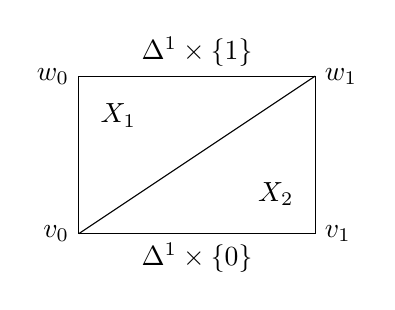
\begin{tikzpicture}
\draw (-1.5,-1) -- (1.5,-1);
\draw (-1.5,1) -- (1.5,1);
\draw (-1.5,-1) -- (-1.5,1);
\draw (1.5,-1) -- (1.5,1);
\draw (0,-1) node[below] {$\Delta^1 \times \{0\}$};
\draw (-1.5,-1) node[left] {$v_0$};
\draw (1.5,-1) node[right] {$v_1$};
\draw (-1.5,1) node[left] {$w_0$};
\draw (1.5,1) node[right] {$w_1$};
\draw (0,1) node[above] {$\Delta^1 \times \{1\}$};
\draw (-1.5,-1) -- (1.5,1);
\draw (-1,0.5) node {$X_1$};
\draw (1,-0.5) node {$X_2$};
\end{tikzpicture}
$$
Then we have
$$P_1(\sigma^1) = F\circ (\sigma^1 \times \id_I) \vert_{[v_0,w_0,w_1]} - F \circ (\sigma^1 \times \id_I)\vert_{[v_0,v_1,w_1]},$$
where $[v_0,w_0,w_1]$ denote the $2$-simplex $X_1$ and $[v_0,v_1,w_1]$ the $2$-simplex $X_2$.

\end{ex}


\begin{ex}
Now illustrate the case $n=2$. Then the prism $\Delta^2 \times I$ is given by

$$
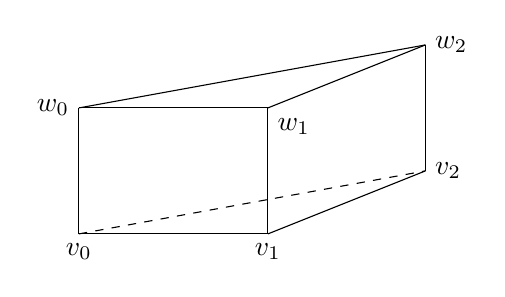
\begin{tikzpicture}[scale=0.8]

\draw (-1.5,0) -- (1.5,0);
\draw (1.5,0) -- (1.5,2);
\draw (1.5,2) -- (-1.5,2);
\draw (-1.5,2) -- (-1.5,0);
\draw[dashed] (-1.5,0) -- (4,1);
\draw (4,1) -- (1.5,0);
\draw (4,1) -- (4,3);
\draw (4,3) -- (-1.5,2);
\draw (1.5,2) -- (4,3);
\draw (-1.5,0) node[below] {$v_0$};
\draw (1.5,0) node[below] {$v_1$};
\draw (4,1) node[right] {$v_2$};
\draw (-1.5,2) node[left] {$w_0$};
\draw (1.5,1.7) node[right] {$w_1$};
\draw (4,3) node[right] {$w_2$};


\end{tikzpicture}
$$
Then we have
$$P_2(\sigma^2) = F \circ ( \sigma^2 \times \id_I) \vert_{[v_0,w_0,w_1,w_2]} - F \circ ( \sigma^2 \times \id_I) \vert_{[v_0,v_1,w_1,w_2]} + F \circ ( \sigma^2 \times \id_I) \vert_{[v_0,v_1,v_2,w_2]}$$
where the $3$-simplex $X_1=[v_0,w_0,w_1,w_2]$ is given by
$$
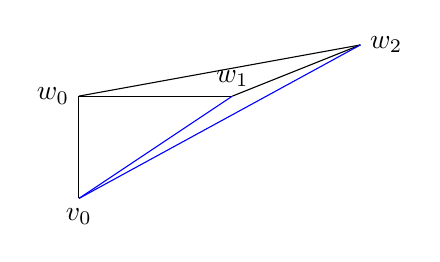
\begin{tikzpicture}[scale=0.65]

\draw (1.5,2) -- (-1.5,2);
\draw (-1.5,2) -- (-1.5,0);
\draw (4,3) -- (-1.5,2);
\draw (1.5,2) -- (4,3);
\draw (-1.5,0) node[below] {$v_0$};
\draw (-1.5,2) node[left] {$w_0$};
\draw (1.5,2) node[above] {$w_1$};
\draw (4,3) node[right] {$w_2$};
\draw[color=blue] (-1.5,0) -- (1.5,2);
\draw[color=blue] (-1.5,0) -- (4,3);

\end{tikzpicture}
$$
the $3$-simplex $X_2=[v_0,v_1,w_1,w_2]$ by



$$
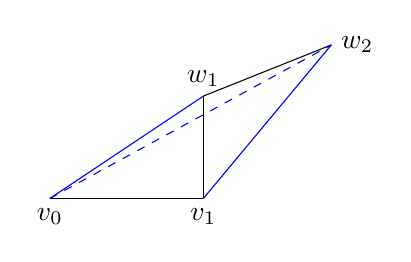
\begin{tikzpicture}[scale=0.65]

\draw (-1.5,0) -- (1.5,0);
\draw (1.5,0) -- (1.5,2);
\draw (1.5,2) -- (4,3);
\draw (-1.5,0) node[below] {$v_0$};
\draw (1.5,0) node[below] {$v_1$};
\draw (1.5,2) node[above] {$w_1$};
\draw (4,3) node[right] {$w_2$};
\draw[color=blue] (1.5,0) -- (4,3);
\draw[color=blue] (-1.5,0) -- (1.5,2);
\draw[color=blue,dashed] (-1.5,0) -- (4,3);


\end{tikzpicture}
$$

and the $3$-simplex $X_3=[v_0,v_1,v_2,w_2]$ by
$$
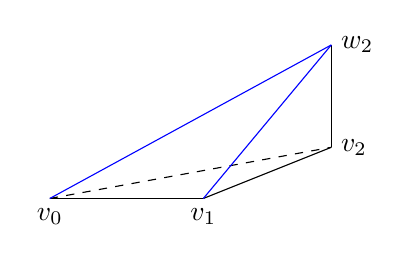
\begin{tikzpicture}[scale=0.65]

\draw (-1.5,0) -- (1.5,0);



\draw[dashed] (-1.5,0) -- (4,1);
\draw (4,1) -- (1.5,0);
\draw (4,1) -- (4,3);

\draw (-1.5,0) node[below] {$v_0$};
\draw (1.5,0) node[below] {$v_1$};
\draw (4,1) node[right] {$v_2$};

\draw (4,3) node[right] {$w_2$};
\draw[color=blue] (-1.5,0) -- (4,3);
\draw[color=blue] (1.5,0) -- (4,3);


\end{tikzpicture}
$$

\end{ex}



Note that $[v_0, \ldots, v_i, w_i, \ldots, w_n] = [v_0, \ldots, v_i] \star [w_i, \ldots, w_n]$ is the joint of two simplices, which consists of all the lines between them. One easily sees that $\Delta^p \star \Delta^q = \Delta^{p+q+1}$. Now we have to show that $P_*$ is an $R$-chain homotopy.

\begin{proposition}
Let $X,Y$ be spaces and $f,g: X \la Y$ be homotopic maps with homotopy $F: X \times I \la Y$. Then the maps $f_*=\Cs_*(f;R),g_*= \Cs_*(g;R): \Cs_*(X;R) \la \Cs_*(Y;R)$ are homotopic as maps of $R$-chains. More precisely, the family 
$$P_* =\{P_n: \Cs_n(X;R) \la \Cs_{n+1}(Y;R)\}_{n \in \Z}$$
satisfies
$$f_n-g_n = P_{n-1} \circ \partial_n + \partial_{n+1} \circ P_n.$$
\begin{pr}
Let $\partial_*$ be the boundaries of $\Cs_*(X;R)$ and $d_n$ those of $\Cs_*(Y;R)$. Then
\begin{alignat*}{5}
d_{n+1}(P_n(\sigma^n)) \ \ &=&& \ \ d_{n+1} \left(\sum_{i=0}^n (-1)^{i} p_n  \vert_{[v_0, \ldots, v_i, w_i, \ldots, w_n]} \right) \\
&=&& \ \ \sum_{i =0}^{n} \left( \sum_{j=0}^{i} (-1)^{i} (-1)^{j} p_n  \vert_{[v_0, \ldots, \hat{v}_j, \ldots, v_i, w_i, \ldots, w_n]} \right) \\
&\hspace{3pt} +&& \ \ \sum_{i=0}^n \left( \sum_{j=i}^{n} (-1)^{i} (-1)^{j+1} p_n \vert_{[v_0, \ldots, v_i, w_i, \ldots, \hat{w}_j, \ldots, w_n]} \right) \\
&=&& \ \ \sum_{i =0}^{n} \left( \sum_{j=0}^{i-1} (-1)^{i} (-1)^{j} p_n \vert_{[v_0, \ldots, \hat{v}_j, \ldots, v_i, w_i, \ldots, w_n]} + p_n \vert_{[v_0, \ldots, v_{i-1}, w_i, \ldots, w_n]} \right) \\
&\hspace{3pt} +&& \ \ \sum_{i=0}^n \left( \sum_{j=i+1}^{n} (-1)^{i} (-1)^{j+1} p_n \vert_{[v_0, \ldots, v_i, w_i, \ldots, \hat{w}_j, \ldots, w_n]}  + p_n \vert_{[v_0, \ldots, v_i, w_{i+1}, \ldots, w_n]}\right) \\
&=&& \ \ p_n \vert_{[w_0, \ldots, w_n]}  + \sum_{i=1}^n \left( \sum_{j=0}^{i-1} (-1)^i(-1)^j p_n  \vert_{[v_0, \ldots, \hat{v}_j, \ldots, v_i, w_i, \ldots, w_n]} \right) \\
&\hspace{3pt} -&& \ \ p_n \vert_{[v_0, \ldots, v_n}] - \sum_{i=0}^{n-1} \left( \sum_{j=i+1}^n (-1)^{i} (-1)^{j+1} F \circ (\sigma^n \times \id_I) \vert_{[v_0, \ldots, v_i, w_i, \ldots, \hat{w}_j, \ldots, w_n]} \right)
\end{alignat*}
Note that
$$p_n \vert_{[v_0, \ldots, v_n]} = \left( F \circ ( \sigma^n \times \id_I)\right) \vert_{[v_0, \ldots v_n]} = F\vert_{X \times \{0\}}(\sigma^n) = f_n(\sigma^n) $$
and analogously
$$p_n \vert_{[w_0, \ldots, w_n]}= g_n(\sigma^n).$$
Then we continue
\begin{alignat*}{5}
d_{n+1}(P_n(\sigma)) \ \ &=&& \ \ g_n(\sigma^n) - f_n(\sigma^n) +
\ \ \sum_{i=1}^n (-1)^{i} \left( \sum_{j=0}^{i-1} (-1)^{j} p_n\vert_{[v_0, \ldots, \hat{v}_j, \ldots, v_i, w_i, \ldots, w_n]}\right) \\
&\hspace{3pt} -&& \sum_{i=0}^{n-1} (-1)^{i} \left( \sum_{j=i+1}^n (-1)^{j+1} p_n  \vert_{[v_0, \ldots, v_i, w_i, \ldots, \hat{w}_j, \ldots, w_n]} \right) \\ 
&=&& \ \ g_n(\sigma^n) - f_n(\sigma^n) +
\ \ \sum_{i=0}^{n-1} (-1)^{i} \left( \sum_{j=0}^{i} (-1)^{j+1} p_n\vert_{[v_0, \ldots, \hat{v}_j, \ldots, v_{i+1}, w_{i+1}, \ldots, w_n]}\right) \\
&\hspace{3pt} -&& \sum_{i=0}^{n-1} (-1)^{i} \left( \sum_{j=i+1}^n (-1)^{j+1} p_n  \vert_{[v_0, \ldots, v_i, w_i, \ldots, \hat{w}_j, \ldots, w_n]} \right) \\ 
&=&& \ \ g_n(\sigma^n) - f_n(\sigma^n) - P_{n-1}(\partial_n(\sigma^n)),
\end{alignat*}
giving the proof. $\hfill \Box$
\end{pr}


\end{proposition}


For general maps of pairs $f,g: (X,A) \la (Y,B)$ homotopic through maps of pairs we obtain 
$$P_n(\Cs_n(A;R)) \subseteq \Cs_{n+1}(B;R).$$
Moreover the relation $\partial_{n+1}\circ P_n = g_n - f_n - P_{n-1}\circ \partial_n$ remains valid. Thus

\begin{theorem}
The pair $(\Hs_*, \partial_*)$ satisfies the axiom of homotopy invariance.
\end{theorem}

\begin{remark}
Let $X,Y$ be homotopy equivalent spaces. Then $\Hs_n(X;R) \cong \Hs_n(Y;R)$ for all $n \in \Z$. 
\begin{pr}
Let $f: X \la Y$ and $g: Y \la X$ such that $ f \circ g \sim_{h_1} \id_Y$ and $g \circ f \sim_{h_2} \id_X$. Then for each $n \in \Z$ we have that 
$$\Hs_n(f_*;R) \circ \Hs_n(g_*;R) = \Hs_n(f_* \circ g_*;R) = \Hs_n(\id_Y;R) = \id_{\Hs_n(\id_Y;R)},$$
$$\Hs_n(g_*;R) \circ \Hs_n(f_*;R) = \Hs_n(g_* \circ f_*;R) = \Hs_n(\id_X;R) = \id_{\Hs_n(\id_X;R)},$$
i.e. $\Hs_n(f_*;R)$ and $\Hs_n(g_*;R)$ are isomorphisms. This implies the assertion. $\hfill \Box$
\end{pr}

\end{remark}


\begin{remark}
Let $f_*, g_*: C_* \la D_*$ satisfy $H_*(f_*) = H_*(g_*)$. Do we have $f_* \sim g_*$?. Answer: No! Not even if $C_*$ and $D_*$ are free over $\mathbb{Z}$. However, if for $f_*:C_* \la D_*$ each $H_*(f_*)$ is an isomorphism and if $C_*$ and $D_*$ are free over a principal ideal domain, then $C_* \sim D_*$.

\end{remark}

















\section{Excision} %PARAGRAPH IV.4




Let $X$ be a space and $\mathcal{U}:= \{U_i\}_{i\in I}$ a family of subspaces such that $\bigcup_{i\in I} \overset{\circ}{U}_i =X$. Let $C_n^{\mathcal{U}}(X;R) \subseteq \Cs_n(X;R)$ be the submodule generated by all $\sigma^n: \Delta^n\la X$ with $\sigma^n(\Delta^n) \subseteq U_i$ for some $i \in I$. An element $c \in C^{\mathcal{U}}_n(X;R)$ is called a $\mathcal{U}$\textit{-small chain}.

\begin{proposition}[small simplices lemma]
The inclusion $i_*: C_*^{\mathcal{U}}(X;R) \hookrightarrow \Cs_*(X;R)$ is a \textit{chain homotopy equivalence}, i.e. there exists a chain map
$$r_*: \Cs_*(X;R) \la C_*^{\mathcal{U}}(X;R)$$
such that $i_* \circ r_* \sim \id_{\Cs_*(X;R)}$ and $r_* \circ i_* \sim \id_{C_*^{\mathcal{U}}(X;R)}$.
\end{proposition}

\begin{theorem}
The pair $(\Hs_*, \partial_*)$ satisfies the axiom of excision.
\begin{pr}
Given a triple $(X,Y;A)$ such that $\overline{A} \subseteq \overset{\circ}{Y}$ let $\mathcal{U} = \{ X \setminus A, Y\}$. Then $\overset{\circ}{(X \setminus A)} \cup \overset{\circ}{Y} =X$. By proposition 4.1 we have a chain homotopy equivalence
$$C_*^{\mathcal{U}} \overset{\overset{i_*}{\la}}{\underset{r_*}{\longleftarrow}} \Cs_*(X;R)$$
We have
$$C_*^{\mathcal{U}}(X;R) = \Cs_*(Y;R) + \Cs_*(X \setminus A;R)$$
and 
$$\Cs_*(Y \setminus A;R) = \Cs_*(B;R) \cap \Cs_*(X\setminus A;R).$$
Then we have
\begin{alignat*}{5}
\Cs_*( X \setminus A, Y \setminus A;R) \ \ &\cong&& \ \ \slant{\Cs_*(X \setminus A;R)}{\Cs_*(Y\setminus A;R)} \\
&\cong&& \ \ \slant{\left( \Cs_*(X \setminus A;R) + \Cs_*(Y;R)\right)}{\Cs_*(Y;R)} \\
&\cong&& \ \ \slant{C_*^{\mathcal{U}}(X;R)}{\Cs_*(Y;R)} \\
& \overset{\sim}{\la}&& \ \ \slant{\Cs_*(X;R)}{\Cs_*(Y;R)}\\
&\cong&& \ \ \Cs_*(X,Y;R).
\end{alignat*}

Now lemma IV.2.5 gives us the proof. $\hfill \Box$
\end{pr}
\end{theorem}


Before we prove the proposition, we want to investigate the dimension axiom.

\begin{theorem}
The pair $(\Hs_*, \partial_*)$ satisfies the dimension axiom.
\begin{pr}
Let $X= \{ \cdot \}$ be a space with one element. Then for all $n \in \mathbb{N}_0$ there exists only one map $\sigma^: \Delta^n \la X$. Thus the chain complex $\Cs_*(X;R)$ looks like
$$\partial_n(\sigma^n) = \sum_{i=0}^n (-1)^{i} \sigma^{n-1}  \ = \ \ \begin{cases} \ \sigma^{n-1}, &  \textrm{ if } n \textrm{ is even } \\  \ 0, & \textrm{ if } n \textrm{ is odd. } \end{cases}$$
and thus
$$\Hs_0(X;R) = R$$
and 
$$\Hs_n(X;R) = \slant{ \ker \partial_n}{\mathrm{im} \ \partial_{n+1}} = \begin{cases} \ \slant{0}{0} \cong 0, & \textrm{ if } n \textrm{ is even,} \\ \slant{R}{R} \cong 0, &\textrm{ if } n \textrm{ is odd,} \end{cases}$$
which proves the claim. $\hfill \Box$

\end{pr}

\end{theorem}

\begin{theorem}
$(\Hs_*, \partial_*)$ is a homology theory with values in $\Rmod$ which satisfies the dimension axiom.
\begin{pr}
Follows by the last four theorems. $\hfill \Box$
\end{pr}
\end{theorem}





\section{Proof of the small simplices lemma} %PARAGRAPH IV.5


\newcommand{\sbar}{\sigma^{\mathrm{bar}}}

We now prove the proposition above. Any $p+1$ points $v_0, \ldots, v_p \in \Delta^q$ define an affine linear map $\Delta^p \la \Delta^q$, $v_i \mapsto \sigma(v_i)$ which by abuse of notation we denote by $\sigma=[v_0, \ldots, v_p]$. Now any other pont $v \in \Delta^q$ defines the cone simplex
$$v\sigma = [v ,v_0, \ldots, v_p]: \Delta^{p+1} \la \Delta^q.$$
Let $L_p(\Delta^q;R) \subseteq \Cs_*(\Delta^q;R)$ be the free submodule the $p$-simplices in $\Delta^q$ as a basis.Then $L_*(\Delta^q;R)$ is a subcomplex. For fixed $v \in \Delta^q$ forming cones on simplices defines an homomorphism of $R$-modules
$$\underline{v}: L_p(\Delta;R) \la L_{p+1}(\Delta^q;R), \qquad \sigma \mapsto v\sigma.$$
For $\sigma=[v_0, \ldots, v_p]$ let 
$$\sbar := \frac{1}{p+1} (v_0 + \ldots + v_p).$$
Now define the \textit{barycenrtic subdivision operator} to be the $R$-linear map
$B_p: L_p(\Delta^q;R) \la L_p(\Delta^q;R)$
defined inductively by
$$B_p(\sigma) = \begin{cases} \ \sigma, & \ \textrm{ for } p=0 \\ \ \underline{\sigma}^{\mathrm{bar}}\left((B_{p-1} \circ \partial_p^{\hspace{1pt}\mathrm{sing}})(\sigma)\right), & \ \textrm{ for }p\geqslant 1. \end{cases}$$

\begin{ex}
For $p=1$ we have $\sigma=[v_0, v_1]$.
Applying the barycentric subdivision operator to $\sigma$ gives us
\begin{alignat*}{5}
B_1(\sigma) \ \ &=&& \ \ \underline{\sigma}^{\mathrm{bar}} \left( B_0( \partial_1^{\hspace{1pt}\mathrm{sing}} ( \sigma))\right) \\
&=&& \ \ \underline{\sigma}^{\mathrm{bar}} \left( B_0([v_1[-[v_0])\right) \\
&=&& \ \ \underline{\sigma}^{\mathrm{bar}} \left( [v_1]-[v_0] \right) \\
&=&& \ \ \left[ \frac{1}{2} (v_0+v_1), v_1\right] - \left[ \frac{1}{2} (v_0+v_1), v_0\right]
\end{alignat*}
Thus we see, what the operator does:
$$
\begin{tikzpicture}
\draw (0,0) -- (0.95,0);
\draw[->] (-0.95,0) -- (0,0);
\draw (-0.95,0) arc(0:360:0.05);
\draw (1.05,0) arc(0:360:0.05);
\draw (1,0) node[below] {$v_1$};
\draw (-1,0) node[below] {$v_0$};
\draw[->] (5.05,0) -- (6,0);
\draw (6,0) -- (6.95,0);
\draw[->] (7.05,0) -- (8,0);
\draw (8,0) -- (8.95,0);
\draw (5.05,0) arc(0:360:0.05);
\draw (7.05,0) arc(0:360:0.05);
\draw (9.05,0) arc(0:360:0.05);
\draw (5,0) node[below] {$v_0$};
\draw (9,0) node[below] {$v_1$};
\draw (7,0) node[below] {$\frac{1}{2} (v_0+v_1)$};

\draw[->] (2.5,0) -- (3.5,0);
\draw (3,0) node[above] {$B_1$};

\end{tikzpicture}
$$
It subdivides $\sigma$ and preserves orientation.

\end{ex}


\begin{ex}
For $p=2$ consider $\sigma =[v_0, v_1, v_2]$. Then 
\begin{alignat*}{5}
B_2(\sigma) \ \ &=&& \ \ \underline{\sigma}^{\mathrm{bar}} \left( B_1(\partial_2^{\hspace{1pt}\mathrm{sing}}([v_0,v_1,v_2]))\right) \\
&=&& \ \ \underline{\sigma}^{\mathrm{bar}} \left( B_1( [v_1,v_2] - [v_0,v_2] + [v_0,v_1])\right) \\
&=&& \ \ \underline{\sigma}^{\mathrm{bar}} \left( \left[\frac{1}{2}(v_1+v_2),v_2\right] - \left[\frac{1}{2}(v_1+v_2),v_1\right] - \left[\frac{1}{2}(v_0+v_2),v_2\right] \right. \\
&&& \qquad + \left. \left[\frac{1}{2}(v_0+v_2),v_0\right] + \left[\frac{1}{2}(v_0+v_1),v_1\right] - \left[\frac{1}{2}(v_0+v_)1,v_0\right] \right)\\
&=&& \ \ \left[\frac{1}{3}\left( v_0, v_1,v_2\right), \frac{1}{2}(v_1+v_2), v_2 \right] - \left[\frac{1}{3}\left( v_0, v_1,v_2\right), \frac{1}{2}(v_1+v_2), v_1 \right]\\
&-&& \ \ \left[\frac{1}{3}\left( v_0, v_1,v_2\right), \frac{1}{2}(v_0+v_2), v_2 \right] + \left[\frac{1}{3}\left( v_0, v_1,v_2\right), \frac{1}{2}(v_0+v_2), v_0 \right] \\
&+&& \ \ \left[\frac{1}{3}\left( v_0, v_1,v_2\right), \frac{1}{2}(v_0+v_1), v_1 \right] - \left[\frac{1}{3}\left( v_0, v_1,v_2\right), \frac{1}{2}(v_0+v_1), v_0 \right]
\end{alignat*}
Illustrated, we obtain 

$$
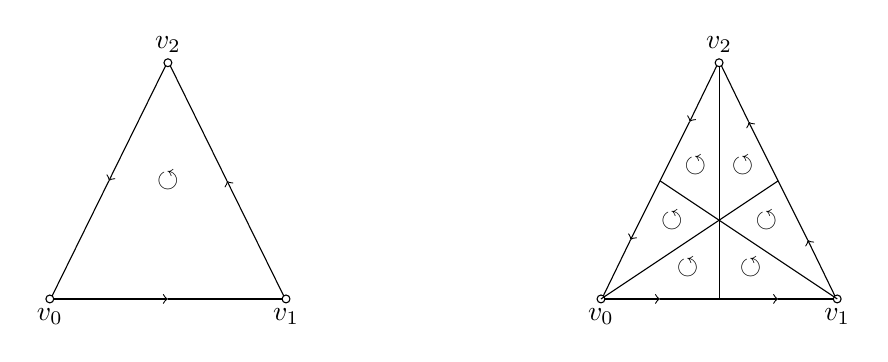
\begin{tikzpicture}


\draw (-2.95,0) arc(0:360:0.05);
\draw (0.05,0) arc(0:360:0.05);
\draw (-1.45,3) arc(0:360:0.05);
\draw[->] (-2.95,0) -- (-1.5,0);
\draw (-1.5,0) -- (-0.05,0);
\draw[->] (-0.03,0.04) -- (-0.75,1.5);
\draw (-0.75,1.5) -- (-1.47,2.96);
\draw[->] (-1.53,2.96) -- (-2.25,1.5);
\draw (-2.25,1.5) -- (-2.97,0.04);
\draw (-3,0) node[below] {$v_0$};
\draw (0,0) node[below] {$v_1$};
\draw (-1.5,3) node[above] {$v_2$};

\draw (-1.5,1.5) node {$\circlearrowleft$};





\draw (4.05,0) arc(0:360:0.05);
\draw (7.05,0) arc(0:360:0.05);
\draw (5.55,3) arc(0:360:0.05);
\draw[->] (4.05,0) -- (4.75,0);
\draw[->] (4.75,0) -- (6.25,0);
\draw (6.25,0) -- (6.95,0);

\draw[->] (6.97,0.04) -- (6.625,0.75);
\draw[->] (6.625,0.75) -- (5.875,2.25);
\draw (5.875,2.25) -- (5.53,2.96);

\draw[->] (5.47,2.96) -- (5.125,2.25);
\draw[->] (5.125,2.25) -- (4.375,0.75);
\draw (4.375,0.75) -- (4.03,0.04);


\draw (4,0) node[below] {$v_0$};
\draw (7,0) node[below] {$v_1$};
\draw (5.5,3) node[above] {$v_2$};
\draw (4,0) -- (6.25,1.5);
\draw (5.5,0) -- (5.5,2.95);
\draw ( 7,0) -- (4.75,1.5);

\draw (5.1,0.4) node {$\circlearrowleft$};
\draw (5.9,0.4) node {$\circlearrowleft$};
\draw (6.1,1.0) node {$\circlearrowleft$};
\draw (4.9,1.0) node {$\circlearrowleft$};
\draw (5.8,1.7) node {$\circlearrowleft$};
\draw (5.2,1.7) node {$\circlearrowleft$};
\end{tikzpicture}
$$
Again we see, that $\sigma$ gets subdivided.
\end{ex}


\begin{lemma}
The operator $B_p$ defines a chain map $B_*$.
\begin{pr}
We have to show that $\partial_p \circ B_p = B_{p-1} \circ \partial_p$. Do this by induction. For $p=0$ this is clear, since $B_{-1} = \partial_0 = 0$. Le now $p \geqslant 1$. Then for $\sigma=[v_0, \ldots, v_p]$ and $v \in \Delta^q$ we have 
$$\partial_{p+1}(v \sigma) = \sigma - \partial_p(\sigma)$$
(homework). Then we calculate
\begin{alignat*}{5}
\partial_p(B_p(\sigma)) \ \ &=&& \ \ \partial_p \left( \underline{\sigma}^{\mathrm{bar}} \left( B_{p-1}(\partial_p(\sigma))\right) \right) \\
&=&& \ \ B_{p-1}(\partial_p(\sigma)) - \underline{\sigma}^{\mathrm{bar}} \left( \partial_{p-1}(B_{p-1}(\partial_p(\sigma)))\right) \\
&=&& \ \ B_{p-1}(\partial_p(\sigma)) - \underline{\sigma}^{\mathrm{bar}} \left( B_{p-2} (\partial_{p-1}(\partial_p(\sigma)))\right) \\
&=&& \ \ B_{p-1}(\partial_p(\sigma))
\end{alignat*}
where we used the induction hypothesis $\partial_{p-1} \circ B_{p-1} = B_{p-2} \circ \partial_{p-1}$ and $\partial_{p-1} \circ \partial_{p}=0$. $\hfill \Box$
\end{pr}
\end{lemma}
From [Hatcher, p.120] or [Bredon, p.226] we know that the simplices in $B_p(\sigma)$ have diameter at most $\frac{p}{p+1} \mathrm{diam} \ \sigma$. \\
Now define $h_*: L_*(\Delta^q;R) \la L_{*+1}(\Delta^q;R)$ by $h_0=0$ and 
$$h_p: L_p(\Delta^q;R) \la L_{p+1}(\Delta^q;R), \qquad \sigma \mapsto \underline{\sigma}^{\mathrm{bar}} \left( B_p(\sigma) - \sigma - h_{p-1}(\partial_p(\sigma))\right)$$
To see what $h_*$ does, we want to illustrate $h_p$ for $p=1$ and $p=2$.


\begin{ex}
For $p=1$ we have $\sigma=[v_0, v_1]$. We have seen what $B_1(\sigma)$ is and $h_0=0$, thus we obtain an image 
$$
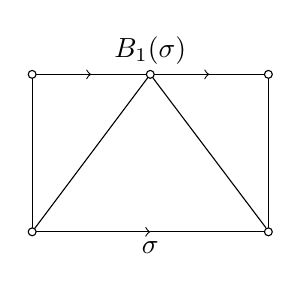
\begin{tikzpicture}
\draw (-1.45,0) arc(0:360:0.05);
\draw (1.55,0) arc(0:360:0.05);
\draw (-1.45,2) arc(0:360:0.05);
\draw (1.55,2) arc(0:360:0.05);
\draw (0.05,2) arc(0:360:0.05);
\draw[->] (-1.45,0) -- (0,0);
\draw (0,0) -- (1.45,0);
\draw[->] (-1.45,2) -- (-0.75,2);
\draw (-0.75,2) -- (-0.05,2);
\draw[->] (0.05,2) -- (0.75,2);
\draw (0.75,2) -- (1.45,2);
\draw (-1.5,0.05) -- (-1.5,1.95);
\draw (1.5,0.05) -- (1.5,1.95);
\draw (-1.47,0.04) -- (-0.03,1.96);
\draw (1.47,0.05) -- (0.03,1.96);
\draw (0,0) node[below] {$\sigma$};
\draw (0,2) node[above] {$B_1(\sigma)$};

\end{tikzpicture}
$$
We want to interpret this as a compatible subdivision of $\sigma$.
\end{ex}

\begin{ex}
For $p=2$ and $\sigma= [v_0, v_1, v_2]$ we have also seen what $B_2(\sigma)$ is and $h_1(\partial(\sigma))$ follows from the preceeding example. We obtain an image (skip the orientations now):



$$
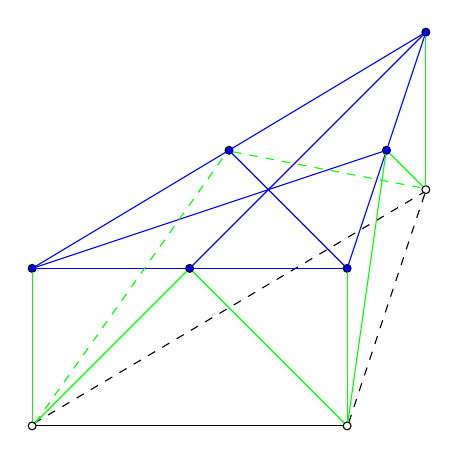
\begin{tikzpicture}


\draw (-1.95,0) arc(0:360:0.05);
\draw (2.05,0) arc(0:360:0.05);
\draw (3.05,3) arc(0:360:0.05);
\draw (-1.95,0) -- (1.95,0);
\draw[dashed] (2.02,0.04) -- (2.99,2.96);
\draw[dashed] (-1.98,0.03) -- (2.98, 2.97);
\draw[fill=blue] (-1.95,2) arc(0:360:0.05);
\draw[fill=blue](2.05,2) arc (0:360:0.05);
\draw[fill=blue] (0.05,2) arc (0:360:0.05);
\draw[fill=blue] (3.05,5) arc(0:360:0.05);
\draw[fill=blue] (2.55,3.5) arc(0:360:0.05);
\draw[fill=blue](0.55,3.5) arc(0:360:0.05);
\draw[color=blue] (-1.95,2) -- (-0.05,2);
\draw[color=blue] (0.05,2) -- (1.95,2);
\draw[color=blue] (2,2) -- (3,5);
\draw[color=blue] (3,5) -- (-2,2);
\draw[color=blue] (0,2) -- (3,5);
\draw[color=blue] (-2,2) -- (2.5,3.5);
\draw[color=blue] (2,2) -- (0.5,3.5);
\draw[color=green] (-2,0.05) -- (-2,1.95);
\draw[color=green] (2,0.05) -- (2,1.95);
\draw[color=green] (-1.96,0.04) -- (-0.04,1.96);
\draw[color=green] (1.96,0.04) -- (0.04,1.96);
\draw[color=green] (3,3.05) -- (3,4.95);
\draw[color=green] (2.01,0.05) -- (2.49,3.45);
\draw[color=green] (2.54,3.46) -- (2.96,3.04);
\draw[color=green,dashed] (-1.96,0.04) -- (0.46,3.46);
\draw[color=green,dashed] (0.55,3.48) -- (2.96,3.02);

\end{tikzpicture}
$$

\begin{lemma}
We have $B_* \sim_{h_*} \id_{L_*(\Delta^q;R)}$.
\begin{pr}
By induction, as above. $\hfill \Box$
\end{pr}
\end{lemma}

$\quad$ Now we observe that $B_*$ gives rise to a natural transformation
$$B_*: \Cs_*(-;R) \la \Cs_*(-;R)$$
with components
$$B(X)_p: \Cs_p(X;R) \la \Cs_p(X;R), \qquad \sigma \mapsto \Cs_p(\sigma;R) \left( B_p(\id_{\Delta^p})\right)$$
It is left to the reader to check that this is well defined. Similarly we obtain 
$$h(X)_p: \Cs_p(X;R) \la \Cs_{p+1}(X;R), \qquad \sigma \mapsto \Cs_{p+1})\sigma;R) \left( h_p(\id_{\Delta^p})\right)$$
One easily checks that $B(X)_* \sim_{h(X)_*} \id_{\Cs_*(X;R)}$. Now by compatibility of chain homotopy with composition we also have 
$$B^k(X)_* \sim B(X)_* \sim B^{k-1}(X)_* \sim \id_* \circ B^{k-1}(X)_* \sim \ldots \sim \id_{\Cs_*(X;R)}$$
An explicit homotopy is given by
$$F_*^k := \sum_{i=0}^{k-1} h(X)_* \circ B^{i}(X)_*.$$
Indeed we have
\begin{alignat*}{5}
\partial_{k+1} \circ F_*^k + F_*^k \circ \partial_k \ \ &=&& \ \ \sum_{i=0}^{k-1} \partial_{k+1}\circ (h(X)_* \circ B^{i}(X)_*) + (h(X)_* \circ B^{i}(X)_* )\circ (\partial_k) \\
&=&& \ \ \sum_{i=0}^{k-1} \partial_{k+1} \circ (h(X)_* \circ B^{i}(X)_*) + (h(X)_* \circ \partial_k )\circ B^{i}(X)_* \\
&=&& \ \ \sum_{i=0}^{k-1} \left( \partial_{k+1} \circ h(X)_*  + h(X)_* \circ \partial_k \right) \circ B^{i}(X)_*\\&=&& \ \ \sum_{i=0}^{k-1} \left( \id_* - B(X)_* \right) \circ B^{i}(X)_* \\
&=&& \ \ \id_* - B^{k}(X)_*
\end{alignat*}
where we used that $B^k(X)_* \sim \id_*$ and simplified the telescopic sum.
\newpage 
\begin{lemma}
For any covering $\mathcal{U}= \{U_i\}_{i\in I}$ of $X$ with $\bigcup_{i\in I} \overset{\circ}{U}_i =X$ and for all $\sigma: \Delta^p \la X$ there exists (a minimal) $k=k(\sigma)$ such that the $k$-fold barycentric subdivision $B^{k}(X)_p(\sigma)$ of $\sigma$ is $\mathcal{U}$-small.

\begin{pr}
Apply the Lebesgue lemma to $\{ \sigma^{-1}(\overset{\circ}{U}_i) \}_{i \in I}$ (note that $\sigma$ is continuous) and use the diameter fact from above. $\hfill \Box$

\end{pr}

\end{lemma}


Now set $F_*(\sigma) := F^{k(\sigma)}_*(\sigma)$. We know that
\begin{alignat*}
\sigma - B^{k(\sigma)}(X)_*(\sigma) \ \ &=&& \ \ \left(\partial_{k(\sigma)+1} \circ F_*^{k(\sigma)}\right)(\sigma) + \left(F_{*-1}^{k(\sigma)} \circ \partial_{k(\sigma)}\right)(\sigma) \\
&=&& \ \ \left( \partial_{k(\sigma)+1} \circ F_*\right)(\sigma) + \left( F_{*-1}^{k(\sigma)}\right)(\sigma).
\end{alignat*}
Then we obtain
$$\partial_{k(\sigma)+1} \circ F_* (\sigma) + F_{*-1} \circ \partial_{k(\sigma)}(\sigma) = \sigma - \left( B^{k(\sigma)}(X)_*(\sigma) + F_{*-1}^{k(\sigma)} \circ \partial_{k(\sigma)}(\sigma) - F_{*-1} \circ \partial_{k(\sigma)}(\sigma) \right) \qquad (*) $$ and thus we define
$$r_*(\sigma) := B^{k(\sigma)}(X)_*(\sigma) + F_{*-1}^{k(\sigma)} \circ \partial_{k(\sigma)}(\sigma) - F_{*-1} \circ \partial_{k(\sigma)}(\sigma). $$
We check that $r_*\left( \Cs_*(X;R)\right) \subseteq C_*^{\mathcal{U}}(X;R)$. This is clear for the first summand and in $F_{*-1}^{k(\sigma)} \left( \partial_{k(\sigma)}(\sigma)\right) - F_{*-1}\left( \partial_{k(\sigma)}(\sigma)\right)$ all but the $\mathcal{U}$-small simplices cancel. Then by $(*)$ we have 
$$\partial_{k(\sigma)+1} \left( F_*(\sigma)\right) + F_{*-1}\left( \partial_{k(\sigma)}(\sigma)\right) = \sigma - r_*(\sigma),$$
i.e. 
\begin{alignat*}{5}
\partial_{k(\sigma)} \circ r_*(\sigma) \ \ &=&& \ \ \partial_{k(\sigma)}(\sigma) - \partial_{k(\sigma)}\left( \partial_{k(\sigma)+1} \left( F_*(\sigma)\right)\right) - \partial_{k(\sigma)}\left( F_{*-1}\left( \partial_{k(\sigma)}(\sigma)\right)\right) \\
&=&& \ \ \partial_{k(\sigma)}(\sigma) - \partial_{k(\sigma)}\left( F_{*-1}\left( \partial_{k(\sigma)}(\sigma)\right)\right) \\
&=&& \ \ r_{*-1} \circ \partial_{k(\sigma)} (\sigma)
\end{alignat*}
and $r_*$ is a chain map and we obtain 
$$\partial_{k(\sigma+1} \circ F_* + F_{*-1} \circ \partial_{k(\sigma)} = \id_* - i_* \circ r_*,$$
in other words $i_* \circ r_* \sim_{F_*} \id_*$. Moreover we have $r_* \circ i_* = \id_*$, since $k(\sigma) = 0$ for every $\sigma \in \C_*^{\mathcal{U}}(X;R)$. Hence the theorem is proved. $\hfill \Box$

\end{ex}











\section{Singular homology in degree zero and one} %PARAGRAPH IV.6




For a topological space $X$ let $\pi_0X$ denote the set of path components of $X$.


\begin{theorem}
For any $n \in \Z$ we have
$$\Hs_n(X;R) = \bigoplus_{ X_{\alpha} \in \pi_0X} \Hs_n(X_{\alpha};R).$$
\begin{pr}
For all $\sigma^n \in \Cs_n(X;R)$ we have that $\sigma^n(\Delta^n)$ is path connected, since $\sigma^n$ is continous. Thus the chain modules split into
$$\Cs_n(X;R) = \bigoplus_{X_{\alpha} \in \pi_0X} \Cs_n(X_{\alpha};R).$$
Moreover we have that 
$$\partial_{n} \left( \Cs_n(X_{\alpha};R)\right) \subseteq \Cs_{n-1}(X_{\alpha};R)$$
for all $n$ and $X_{\alpha} \in \pi_0X$, which proves the claim. $\hfill \Box$

\end{pr}

\end{theorem}



\begin{corollary}
The homology theory $(\Hs_*, \parts)$ satisfies the additivity axiom: For a disjoint union $X= \amalg_{i \in I} X_i$ the inclusions $\iota_i: X_i \hookrightarrow X$ induce isomorphisms
$$\Hs_n(X;R) \cong \bigoplus_{i \in I} \Hs_n(X_i; R).$$



\end{corollary}


\begin{remark}
\begin{compactenum}
\item Every homology theory satisfies finite additivity (see homework).
\item The functor $\Hs_n(-,-;R)$ does not preserve general colimits in $\topsp$.

\end{compactenum}

\end{remark}


\begin{theorem}
Let $X$ be a topological space with $n$ path components. Then 
$$\Hs_0(X;R) \cong R^n.$$
\begin{pr}
By the above it suffices to show, that for any path connected space we have $\Hs_0(X;R) \cong R$. Consider the map
$$\epsilon: \Cs_0(X;R)  \la R, \qquad \sum_{i \in I} r_i \sigma_{i}^{0} \mapsto \sum_{i \in I} r_i.$$
We claim that $\ker \epsilon = \im \partial_1$.
\begin{compactenum}
\item["$\supseteq$"] For $\sigma^0 \in \im \partial_1$ write $\sigma^0 = \partial_1(\sigma^1)$. Then 
$$\epsilon(\sigma^1)=\epsilon\left( \partial_1(\sigma^1)\right)= \epsilon \left( \sigma^1\vert_{[v_1]} - \sigma^1 \vert_{[v_0]} \right) = 1-1 = 0,$$
i.e. $\sigma^0 \in \ker \epsilon$.
\item["$\subseteq$"] Let now $\sum_{i \in I} r_i \sigma_i^{0} \in \ker \epsilon$, i.e. the coefficients sum up to zero. Fix $x_0 \in X$. Pick paths $\gamma_i: I \la X$ with $\gamma_i(0) = x_0$ and $\gamma_i(1) = \sigma_i^{0}(v_0)$ for all $i \in I$ (note that this actually is possible since $X$ is path connected). Then each $\gamma_i$ can be interpreted as $\sigma_i^{1}: \Delta^1 \la X$. Then we obtain 
\begin{alignat*}{5}
\partial_1 \left( \sum_{i \in I} r_i \sigma_i^{1} \right)(v_0) \ \ &=&& \ \ \sum_{k \in I} r_i \sigma_i^{1}\vert([v_1]) - \sum_{i \in I} r_i \sigma_i^{1}([v_0]) \\
&=&& \ \ \sum_{i \in I} r_i \gamma_i(1) - \left( \sum_{i \in I} r_i \right) x_0 \\
&=&& \ \ \sum_{i \in I} r_i \sigma_i^{0}(v_0),
\end{alignat*}
thus $\sum_{i \in I} r_i \sigma_i^{0} \in \im \partial_1$.

\end{compactenum}
Now clearly $\epsilon$ is surjective. Further, it is a general fact that $\ker \partial_0 = \Cs_0(X;R)$. Thus by the isomorphism theorem we have
$$R = \im \epsilon \cong \slant{\Cs_0(X;R)}{\ker \epsilon} \cong \slant{\Cs_0(X;R)}{\im \partial_1} \cong \slant{\ker \partial_0}{\im \partial_1} = \Hs_0(X;R),$$
which finishes the proof. $\hfill \Box$

\end{pr}

\end{theorem}


Now let $X \neq \emptyset$. Note that $f: I \la X$ considered as $f: \Delta^1 \la X$ is a cycle if and only if it is a loop, i.e. $f(0) = f(1)$. 


\begin{theorem}[Hurewicz theorem in degree one]

Let $X$ be a topological space, $x_0 \in X$. Then the assignment
$$\mathrm{Hur:} \ \pi_1(X,x_0) \la \Hs_1(X;\Z), \qquad [f] \mapsto f+ B_1^{\mathrm{sing}}(X;\Z)$$
gives a well-defined homomorphism of groups. If $X$ is path connected, then $\mathrm{Hur}$ descends to an isomorphism
$$\mathrm{Hur}_{\mathrm{ab}}: \pi_1(X,x_0) \la \Hs_1(X;\Z).$$
In other words $\ker \mathrm{Hur} = [\pi_1(X,x_0), \pi_1(X,x_0)]$.
\begin{pr}
We first show well-definedness of $\mathrm{Hur}$. Observe that for $f \equiv x_0$ we have $f \in B_1^{\mathrm{sing}}(X;\Z)=: B_1$, since $f+ B_1 \in \im \left( \Hs_1 \left( ( \{x_0\};\Z) \la \Hs_1(X;\Z)\right); \Z\right)$. Let $f \sim_F g$ be homotopic. Then subdivide $I \times I$ as follows:

$$
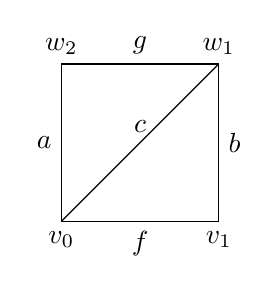
\begin{tikzpicture}

\draw (-2,0) -- (0,0) -- (0,2) -- (-2,2) -- (-2,0);
\draw (-2,0) -- (0,2);
\draw (-2,0) node[below] {$v_0$};
\draw (0,0) node[below] {$v_1$};
\draw (0,2) node[above] {$w_1$};
\draw (-2,2) node[above] {$w_2$};
\draw (-1,1) node[above] {$c$};
\draw (-2,1) node[left] {$a$};
\draw (0,1) node[right] {$b$};
\draw (-1,0) node[below] {$f$};
\draw (-1,2) node[above] {$g$};



\end{tikzpicture}
$$
Let $\sigma_1 = F\vert_{[v_0,w_0,w_1]}$ and $\sigma_2 ) F\vert_{[v_1,v_1,w_1]}$. Then 
$$\partial_2 (\sigma_1 - \sigma_2) = g-c + a-b + c-f = (g-f) + (a-b) = g - f \in B_1,$$
where the last equality holds since $f\equiv x_0$. \\
Now let us show that $\mathrm{Hur}$ is homomorphic. Let $[f], [g] \in \pi_1(X,x_0)$. Consider
$$\sigma^2: \Delta^2 = [v_0, v_1, v_2] \xrightarrow{\textrm{orthogonal projection}} [v_0, v_2] \xrightarrow{f \star g} X.$$
We have 
$$\partial_2 ( \sigma^2) = g-f\star g + f,$$
thus $f+g-f \star g \in B_1$. Similarly we have $f^{-} - (-f) \in B_1$, where $f^{-}$ denotes the reversed path. Assume now $X$ is path connected. We now show that $\mathrm{Hur}_{\mathrm{ab}}$ is an isomorphism. For all $x \in X$ pick paths $\gamma_x$ from $x_0$ to $x$, where $\gamma_{x_0}$ is supposed to be the constant loop. Define
$$\psi: \Cs_1(X;\Z) \la \pi_1(X,x_0)_{\mathrm{ab}}, \qquad f \mapsto \left[ \gamma_{f(0)} \star f \star \gamma_{f(1)}^{-} \right]_{\mathrm{ab}}.$$
Then $\psi$ descends to a homomorphism
$$\overline{\psi}: \Hs_1(X; \Z) \la \pi_1(X,x_0)_{\mathrm{ab}}.$$
Indeed for a singular $2$-simplex $\sigma:= \sigma^2: \Delta^2 \la X$ we have
$$\partial_2(\sigma) = f-g+h$$
and 
\begin{alignat*}{5}
\psi(\partial_2(\sigma)) \ \ &=&& \ \ \psi(f-g+h) \\
&=&&  \ \ \psi(f) - \psi(g) + \psi(h) \\
&=&& \ \ \left[ \gamma_{\sigma(v_1)} \star f \star \gamma_{\sigma(v_2)}^{-} \right]_{\mathrm{ab}} - \left[ \gamma_{\sigma(v_0)} \star g \star \gamma_{\sigma(v_2)}^{-} \right]_{\mathrm{ab}} + \left[ \gamma_{\sigma(v_0)} \star h \star \gamma_{\sigma(v_1)}^{-} \right]_{\mathrm{ab}} \\
&=&& \ \ \left[ \gamma_{\sigma(v_1)} \star f \star g^{-} \star h \star \gamma_{\sigma(v_1)}^{-}\right]_{\mathrm{ab}} \\
&=&& \ \ \id
\end{alignat*}
We now show that $\mathrm{Hur}_{\mathrm{ab}}$ and $\overline{\psi}$ are inverse to ech other. For a loop $[f]_{\mathrm{ab}}$ we clearly have
$$\left( \overline{\psi} \circ \mathrm{Hur}_{\mathrm{ab}} \right) ([f]_{\mathrm{ab}}) = \overline{\psi}(f + B_1)= \left[ \gamma_{f(0)} \star f \star \gamma_{f(1)}^{-}\right]_{\mathrm{ab}} = [f]_{\mathrm{ab}}$$
Note that $x \mapsto \gamma_x$ estends to an $R$-linear map $\gamma: \Cs_0(X;\Z) \la \Cs_1(X;\Z)$ and we have
$$\left( \mathrm{Hur}_{\mathrm{ab}} \circ \psi\right)(c) = c + \gamma ( \partial c) + B_1$$
for $c \in \Cs_1(X;\Z)$. Then
$$\left( \mathrm{Hur}_{\mathrm{ab}} \circ \right)(c+ B_1) = z + \gamma( \partial z) + B_1 = z + B_1,$$
since $\partial z=0.$ $\hfill \Box$

\end{pr}

\end{theorem}









































\chapter{Homology: Computations and applications} %KAPITEL V
\setlength\abovedisplayshortskip{0pt}
\setlength\belowdisplayshortskip{10pt}
\setlength\abovedisplayskip{10pt}
\setlength\belowdisplayskip{10pt}




In this chapter we want to deduce properties of arbitrary homology theories. Thus we will use the axioms of homology only. Let $(H_*, \partial_*)$ be an arbitrary homology theory with values in $\Rmod$.


\section{Relative vs. absolute homology} %PARAGRAPH V.1

\thispagestyle{empty}

First of all a convenient result from algebra:


\begin{lemma}[$5$-lemma]
Suppose the diagram

$$
\begin{xy}
\xymatrix{
 A \ar[rr]^{i} \ar[d]_{\alpha} && B \ar[rr]^{j} \ar[d]_{\beta} && C \ar[rr]^{k} \ar[d]_{\gamma} && D \ar[rr]^{l} \ar[d]_{\delta} && E \ar[d]_{\epsilon} \\
 A' \ar[rr]_{i'} && B' \ar[rr]_{j'} && C' \ar[rr]_{k'} && D' \ar[rr]_{l'} && E'
 }
 \end{xy}
 $$
has exact rows, $\alpha$ is surjective, $\epsilon$ is injective and $\beta, \delta$ are isomorphisms. Then $\gamma$ is an isomorphism as well.
\begin{pr}
We first show that $\gamma$ is injective. Let $c \in \ker \gamma$. We have to show that $c=0$. We have 
$$0= (k' \circ \gamma)(c) = (\delta \circ k)(c),$$ 
and since $\delta$ is an isomorphism, in particular injective, we have $k(c)=0$, i.e. $c \in \ker k = \im j$, write $c=j(b)$. Now we have $0= \gamma(c)=(\gamma \circ j)(b) = (j' \circ \beta)(b)$, i.e. $\beta(b) \in \ker j'= \im i'$, write $\beta(b) =i'(a')$ for some $a' \in A'$. Since $\alpha$ is surjective, we find a preimage $a \in A$ with $\alpha(a) = a'$. Further
$$\beta \left( b - i(a)\right) = \beta(b) - \beta(i(a)) = \beta(b) - i'(\alpha(a)) = \beta(i(a)) - \beta(i(a)) = 0,$$
i.e. $b-i(a) \in \ker \beta$. Since $\beta$ is an isomorphism, in particular injective, we obtain $b-i(a)=0$, thus $b=i(a)$. But then $b \in \im i = \ker j$ and $c= j(b)=0$, which we wanted to show. \\
Now show that $\gamma$ is surjective. Let $c' \in C'$. Since $\delta$ is an isomorphism, in particular surjective, there is $d \in D$ such that $\delta(d)= k'(c')$. Now clearly $l'(k'(c'))= 0$, i.e. 
$$0=(l'(k'(c'))= (l' \circ \delta)(d) = (\epsilon \circ l)(d).$$
Since $\epsilon$ is injective, we must have $l(d)=0$, i.e. $d \in \ker l = \im k$, write $d= k(c)$ for some $c \in C$. Then 
$$\delta(d) =(\delta \circ k)(c) = (k' \circ \gamma)(c).$$
Now $$k'(c'-\gamma(c)) = k'(c') -k'(\gamma(c)) = \delta(d) - \delta(k(c)) = \delta(d) - \delta(d)=0,$$ thus we have $c'-\gamma(c) \in \ker k' = \im j'$, write $c'-\gamma(c) = j'(b')$ for some $b' \in B'$. Since $\beta$ is an isomorphism, in particular surjective, we can write $b'= \beta(b)$ for some $b \in B$. But then 
$$c'-\gamma(c)=(j' \circ \beta)(b)= (\gamma \circ j)(b)= \gamma( j(b)),$$
and this gives $c' = \gamma(j(b)) + \gamma(c) = \gamma( j(b) + c)$ and $\gamma$ is surjective. $\hfill \Box$

\end{pr}


\end{lemma}


Now recall that a map of paris $(X,A) \la (Y,B)$ induces a map of long exact sequences

$$
\begin{xy}
\xymatrix{
 \ldots \ar[r] & H_n(A) \ar[r] \ar[d]_{H_n(f\vert_A)} & H_n(X) \ar[d]_{H_n(f)} \ar[r] & H_n(X,A) \ar[d]_{H_n(f)} \ar[r]^{\partial_n} & H_{n-1}(A) \ar[d]_{H_{n-1}(f\vert_A)} \ar[r] & H_{n-1}(X) \ar[d]_{H_{n-1}(f)} \ar[r] & \ldots \\
 \ldots \ar[r] & H_n(B) \ar[r] & H_n(Y) \ar[r] & H_n(Y,B) \ar[r] & H_{n-1}(B) \ar[r] & H_{n-1}(Y) \ar[r] & \ldots
}
\end{xy}
$$


\begin{corollary}

Let $(X,A)$ and $(Y,B)$ be pairs of spaces and $f: (X,A) \la (Y,B)$ a map of pairs. Consider the families
$$\{H_*({f\vert_A)} : H_*(A) \la H_*(B) \}, \qquad \{H_*(f): H_*(X) \la H_*(Y) \},$$
$$ \{ H_*(f): H_*(X,A) \la H_*(Y,B) \}.$$
If two of them consist of isomorphisms only, then so does the third.
\end{corollary}

\begin{theorem}[triple sequence]
Let $A \subseteq B \subseteq X$ be a triple of spaces. Then there is a long exact sequence
$$\ldots \rightarrow H_n(B,A) \xrightarrow{H_n(i)} H_n(X,A) \xrightarrow{H_n(j)} H_n(X,B) \xrightarrow{\partial} H_{n-1}(B,A) \rightarrow H_{n-1}(X,A) \rightarrow \ldots$$
where $i: (B,A) \hookrightarrow (X,A)$ and $j: (X,A) \hookrightarrow (X,B)$.

\begin{pr}
Define $\partial_n(X,B,A): H_n(X,B) \la H_{n-1}(B,A)$ as the composition
$$H_n(X,B) \xrightarrow{\partial(X,B)} H_{n-1}(B) \xrightarrow{H_{n-1}(l)} H_{n-1}(B,A),$$
where $l: (B, \emptyset) \hookrightarrow (B,A)$. This defines a complex. Indeed consider
$$
\begin{xy}
\xymatrix{
H_n(B,A) \ar[r] \ar[rd] & H_n(X,A) \ar[r] & H_n(X,B) \\
& H_n(B,B)\ar[ru] &
}
\end{xy}
$$ 
According to the long exact sequence of $(B,B)$:
$$\ldots \rightarrow H_n(B) \xrightarrow{\id} H_n(B) \xrightarrow{0} H_n(B,B) \xrightarrow{0} H_{n-1}(B) \rightarrow \ldots$$
we have $H_n(B,B) = 0$. Thus $H_n(j) \circ H_n(i)=0$. Next consider
$$
\begin{xy}
\xymatrix{
H_n(X,A) \ar[rr]^{H_n(j)} \ar[dd]_{\partial_n(X,A)} && H_n(X,B) \ar[dd]^{\partial_n(X,B)} \ar[rrd]^{\partial_n(X,B,A)} \\ &&&&H_{n-1}(B,A) \\ H_{n-1}(A) \ar[rr] && H_{n-1}(B) \ar[rru]&& 
}
\end{xy}
$$
The triangle commutes by definition of $\partial_n(X,B,A)$, the square by functoriality of $H_n$. But the composition at the bottom is zero - thus $\partial_n(X,B,A) \circ H_n(j)=0$. Similarly the diagram
$$
\begin{xy}
\xymatrix{
H_n(X,B) \ar[rr]^{\partial_n(X,B,A)} \ar[dd]_{\partial_n(X,B)} && H_{n-1}(B,A) \ar[dd] \ar[rrd]^{H_{n-1}(i)} &&  \\&&&&H_{n-1}(X,A)\\ H_{n-1}(B) \ar[rr] && H_{n-1}(A) \ar[rru] && \\
}
\end{xy}
$$
gives us $H_{n-1}(i) \circ \partial_n(X,B,A)=0$. To show exactness consider the braid diagram

$$
\begin{xy}
\xymatrix@C=0.4em{
H_{n+1}(X,B) \ar@/^{26pt}/[rr] \ar[rd] && H_n(B,A) \ar[rd] \ar@/^{26pt}/[rr] && H_{n-1}(A) \ar[rd] \ar@/^{26pt}/[rr] && H_{n-1}(X) \ar[rd] & \\
& H_n(B) \ar[ru] \ar[rd] && H_n(X,A) \ar[rd] \ar[ru] && H_{n-1}(B) \ar[rd] \ar[ru] && H_{n-2}(A) \\
H_n(A) \ar[ru] \ar@/_{26pt}/[rr] && H_n(X) \ar[ru] \ar@/_{26pt}/[rr] && H_n(X,B) \ar[ru] \ar@/_{26pt}/[rr] && H_{n-1}(B,A) \ar[ru]&
}
\end{xy}
$$
\textrm{} \\

in which three strings are exact (the long exact sequences of $(B,A), (X,A)$ and $(X,B)$ and in the fourth string the composition of two arrows is zero. The rest is diagram chase (for more see Bredon, IV.6.16). $\hfill\Box$



\end{pr}




\end{theorem}


\begin{defin}
The \textit{reduced homology} of a nonempty topological space $X$ is 
$$\tilde{H}_n(X) := \ker \left(p: H_n(X) \la H_n(\{\cdot\}) \right),$$
induced by $p: X \la \{\cdot \}$. 

\end{defin}


\begin{remark}
\begin{compactenum}
\item A map $f: X \la Y$ gives us the diagram
$$
\begin{xy}
\xymatrix{
\tilde{H}_n(X) = \ker p \ar[rr]^{i_p} \ar[d]{\tilde{H}_n(f)} && H_n(X) \ar[d]_{H_*(f)} \ar[rr]^{p} && H_n(\{\cdot\}) \\
\tilde{H}_n(Y) = \ker q \ar[rr]_{i_q} && H_n(Y) \ar[rru]_{q} &&
}
\end{xy}
$$
For $x \in \ker p$ we have 
$$ (q \circ i_q)(\tilde{H}_n(f)(x)) = q \left(H_n(f) (\circ i_p(x))\right)  = q \left( H_n(f)(x)\right) = 0,$$
thus $\tilde{H}(\cdot)$ is functorial.
\item Let $x_0 \in X$. Then $r: X \la \{x_0\}$ is a retraction, thus the boundaries in the long exact sequence of the pair $(X, \{x_0\})$ vanish. This gives us short exact sequences
$$
\begin{xy}
\xymatrix{
0 \ar[r]& H_n(\{x_0\}) \ar[r]^{\alpha} & H_n(X) \ar@/^{20pt}/[l]^{H_n(r)} \ar[r]^{\beta} & H_n(X, \{x_0\}) \ar@/^{20pt}/[l]^{s} \ar[r] & 0
}
\end{xy}
$$
where $H_n(r)$ with the property $H_n(r) \circ \alpha = \id$ makes the sequence split. By problem 8.1 this gives us $s$ and we obtain a short exact sequence in the other direction. Then 
$$\tilde{H}_n(X) = \ker H_n(r) = \im s \cong H_n(X, \{x_0\})$$
for all $n \in \Z$ and thus
$$H_n(X) \cong H_n(X, \{x_0\}) \oplus H_n(\{x_0\}) \cong \tilde{H}_n(X) \oplus H_n(\{x_0\}).$$

\item If $(H_*, \partial_*)$ satisfies the dimension axiom, we have

$$H_n(X) =\ \ \begin{cases} \ \tilde{H}_0(X) \oplus R, & \ \textrm{ for }n=0 \\ \  \tilde{H}_n(X), & \ \textrm{ else. } \end{cases}$$

In particular we have $\tilde{H}_*(\{\cdot\}) = 0$. 

\item Let $f: X \la Y$ be a nullhomotopic map between two spaces. Then $\tilde{H}_n(f)=0$ for all $n \in \Z$. Indeed, if $f$ is nullhomotopic, $f$ factors as
$$
\begin{xy}
\xymatrix{
X \ar[rd] \ar[rr]^f &&Y \\ & \{*\} \ar[ru] & 
}
\end{xy}
$$
and since $\tilde{H}_n(-;R)$ is functorial and $\tilde{H}_n(\{*\})=0$, $\tilde{H}_n(f)$ factorizes over $0$, thus is zero.
\end{compactenum}
\end{remark}



\begin{proposition}
Let $(X,A)$ be a nonempty, closed neighbourhood deformation retract (CNDR). Then the collapse map $q: (X,A) \la \left( \slant{X}{A}, \slant{A}{A} \right)$ induces isomorphisms
$$H_*(X,A) \overset{\sim}{\la} H_*\left( \slant{X}{A}, \slant{A}{A} \right) \cong \tilde{H}_*\left( \slant{X}{A} \right).$$

\begin{pr}
Let $V \subseteq X$ open such that $V$ deformation retracts onto $A$. Then we have a diagram
$$
\begin{xy}
\xymatrix{
H_n(X,A) \ar[rr]^{\sim} \ar[d]_{q*} && H_n(X,V) \ar[d]_{q_*} && H_n \left( X \setminus A, V \setminus A \right) \ar[ll]^{\sim}_{\mathrm{exc.}} \ar[d]_{q_*} \\
H_n\left( \slant{X}{A}, \slant{A}{A} \right) \ar[rr]^{\sim} && H_n \left( \slant{X}{A}, \slant{V}{A} \right) && H_n \left( \slant{X}{A} \setminus \slant{A}{A}, \slant{V}{A} \setminus \slant{A}{A} \right) \ar[ll]_{\sim}
}
\end{xy}
$$
Since $(VA) \sim (A,A)$, the first horizontal maps are isomorphisms by the triple sequence of $(X,V,A)$ and $\left( \slant{X}{A}, \slant{V}{A}, \slant{A}{A} \right)$, since $(V,A) \sim (A,A)$ and $\left( \slant{V}{A}, \slant{A}{A}\right) \sim \left( \slant{A}{A}, \slant{A}{A}\right)$. The right horizontal maps are isomnorphisms by excision. The right vertical map is an isomorphism since it is induced by a homeomorphism (on the complement of $A$). Then The left vertical arrow is the desired isomorphism to $H_n\left( \slant{X}{A}, \slant{A}{A}\right) \cong \tilde{H}_n\left(\slant{X}{A}\right)$. $\hfill \Box$
\end{pr}



\end{proposition}



\begin{theorem}
Let $(X,A)$ be a closed neighbourhood deformation retract (CNDR). Then we have a natural long exact sequence
$$\ldots \la \tilde{H}_n(A) \la \tilde{H}_n(X) \la \tilde{H}_n\left( \slant{X}{A}\right) \xrightarrow{\partial} \tilde{H}_{n-1}(A) \la \ldots. $$
\begin{pr}

Apply proposition 1.6 to the triple sequence of $(X,A,\{x_0\})$ for some $x_0 \in X$. $\hfill \Box$

\end{pr}

\end{theorem}


\begin{corollary}
Suppose $(H_*, \partial_*)$ satisifes the dimension axiom. Then 
$$H_k(\mathbb{D}^n, \mathbb{S}^{n-1}) \cong \tilde{H}_k(\mathbb{S}^n) \cong \ \begin{cases} \ R, & \textrm{ for }k=n\\ \ 0,& \textrm{ otherwise } \end{cases}$$
\begin{pr}
Let $(X,A) = (\mathbb{D}^n, \mathbb{S}^{n-1})$. Then $(X,A)$ is a nonempty CNDR. Since $\tilde{H}_n(\mathbb{D}^n)=0$ for all $n \in \Z$, the reduced long exact sequence gives us
$$\tilde{H}_k(\mathbb{S}^{n}) \cong \tilde{H}_k\left( \slant{\mathbb{D}^n}{\mathbb{S}^{n-1}} \right) \xrightarrow[\sim]{\partial} \tilde{H}_{k-1}(\mathbb{S}^{n-1}).$$
This is the step $n-1 \mapsto n$ of an induction. For the beginning we have
$$\tilde{H}_k(\mathbb{S}^0) = H_k(\{-1,1\}, \{1\}) \overset{exc.}{\cong} H_k(\{-1\}) \cong \ \begin{cases} \ R, & \textrm{ for } k=0,\\ \ 0, & \textrm{ otherwise }\end{cases}$$
Now we get 
$$\tilde{H}_k(\mathbb{S}^n) \cong \tilde{H}_{k-n}(\mathbb{S}^0) \cong \begin{cases} \  R, & \textrm{ if }k=n, \\ \ 0, & \textrm{ otherwise,} \end{cases}$$
which finishes the proof. $\hfill \Box$

\end{pr}



\end{corollary}







\section{The equivalence of simplicial and singular homology} %PARAGRAPH V.2




\begin{proposition}
The $R$-module $\Hs_n(\Delta^n, \partial \Delta^n;R) \cong R$ is generated by $\id_{\Delta^n}$.
\begin{pr}
Clearly $\id_{\Delta^n}: \Delta^n \la \Delta^n$ is a relative singular cycle. By induction we prove that it generates $\Hs_n(\Delta^n, \partial \Delta^n;R)$. The cases $n=0$ is clear.
Let $\Lambda_0:= \partial \Delta^n \setminus [v_1, \ldots, v_n]$ be the $0$-th horn. Then the triple sequence of $(\Delta^n, \partial \Delta^n,\Lambda_0)$ looks like
$$
\begin{xy}
\xymatrix@C=0.7em{
\ldots \rightarrow \Hs_n(\partial \Delta^n, \Lambda_0) \ar[r] & \Hs_n(\Delta^n, \Lambda_0) \ar[r] & \Hs_n(\Delta^n, \Lambda_0) \ar[r] & H_{n-1}(\partial \Delta^n, \Lambda_0) \ar[r] & H_{n-1}(\Delta^n, \Lambda_0) \ar[r] & \ldots
}
\end{xy}
$$
But since $(\Delta^n, \Lambda_0) \sim (\Lambda_0, \Lambda_0)$the homology modules $H_n(\Delta^n, \Lambda_0;R)$ vanish and by exactness we obtain
$$\Hs_n(\Delta^n, \partial \Delta^n;R) \cong \Hs_{n-1}(\partial \Delta^n, \Lambda_0;R)$$
Now
\begin{alignat*}{5}
\Hs_n(\Delta^n, \partial_n \Delta^n) \ \ &\overset{1.6}{\cong} && \ \ \tilde{H}^{\mathrm{sing}}_{n-1} \left( \slant{\partial_n \Delta^n}{\Lambda_0}\right)\\
&\cong && \ \ \tilde{H}^{\mathrm{sing}}_{n-1}\left(\slant{\Delta^{n-1}}{\partial_{n-1} \Delta^{n-1}}\right)\\
&\overset{1.6}{\cong} && \ \ \Hs_{n-1}(\Delta^{n-1}, \partial_{n-1} \Delta^{n-1})
\end{alignat*}
and since $\id_{\Delta^n}$ maps to $\pm \id_{\Delta^{n-1}}$ along these isomorphisms, $\id_{\Delta^n}$ generates $\Hs_n(\Delta^n, \partial \Delta^n)$. $\hfill \Box$


\end{pr}
\end{proposition}



Let now $(X,A)$ be a $\Delta$-pair. Then we have a canonical homomorphism $H^{\Delta}_n(X,A;R) \la \Hs_n(X,A,R)$ induced by the chain map
$$C^{\Delta}_n(X,A;R) \la \Cs_n(X,A;R), \qquad \sigma_{\alpha}^n \mapsto \sigma_{\alpha}^n.$$

\begin{theorem}
Let $(X,A)$ be a $\Delta$-pair. Then the homomorphisms $H^{\Delta}_n(X,A;R) \la \Hs_n(X,A;R)$ are isomorphisms for all $n \in \Z$.
\begin{pr}
First suppose $A= \emptyset$. Let $X^k$ be the $k$-skeleton of $X$, i.e. the set of all simplices of $X$ of dimension less or equal to $k$.  We obtain a map of long exact sequences
$$
\begin{xy}
\xymatrix@C=1em{
\ldots \ar[r] & H_{n-1}^{\Delta}(X^{k}, X^{k-1}) \ar[d] \ar[r] & H_n^{\Delta}(X^{k-1}) \ar[d] \ar[r] & H_n^{\Delta}(X^k) \ar[r] \ar[d] & H_n^{\Delta}(X^k,X^{k-1}) \ar[d]_{\phi_n} \ar[r]^{\partial} & H_{n+1}^{\Delta}(X^{k-1}) \ar[d] \ar[r] & \ldots \\
\ldots \ar[r] & \Hs_{n-1}(X^k,X^{k-1}) \ar[r] & \Hs_n(X^{k-1}) \ar[r] & \Hs_n(X^k) \ar[r] & \Hs_n(X^k, X^{k-1}) \ar[r]^{\partial} & \Hs_{n+1}(X^{k-1}) \ar[r] & \ldots
}
\end{xy}
$$
We first show, that the homomorphisms $H_n^{\Delta}(X^k) \la \Hs_n(X^k)$ are isomorphisms. We proceed by induction. Th case $k=0$ is clear. Using corollary V.1.2 it now suffices to show that $\phi_n$ is an isomorphism for all $n \in \mathbb{N}$. By definition of the $k$-skeleton we have 
$$C_n^{\Delta}(X^k, X^{k-1};R) \cong \ \begin{cases} \ \bigoplus_{\sigma_{\alpha}^k \in X} \sigma_{\alpha}^k R, & \textrm{ if } k=n, \\ \ 0, & \textrm{ otherwise} \end{cases}$$
Thus all the boundary maps are the zero maps and the homology modules agree with the chain modules:
$$H_n^{\Delta}(X^k, X^{k-1};R) \cong \ \begin{cases} \ \bigoplus_{\sigma_{\alpha}^k \in X} \sigma_{\alpha}^k R, & \textrm{ if } k=n, \\ \ 0, & \textrm{ otherwise} \end{cases}$$
Now let $\phi = \amalg_{\alpha} \sigma_{\alpha}^k$. We obtain a commuting diagram
$$
\begin{xy}
\xymatrix{
\coprod_{\alpha} \left( \Delta_{\alpha}^k, \partial \Delta_{\alpha}^k \right) \ar[rr]^{\phi} \ar[d] && (X^k, X^{k-1}) \ar[d] \\ \left(\slant{\coprod \Delta_{\alpha}^k}{\coprod_{\alpha} \partial \Delta_{\alpha}^k} \right) \ar[rr]^{\sim} && \left( \slant{X^k}{X^{k-1}}, \star \right) 
 }
\end{xy}
$$
By proposition 1.6, $\Hs_n(\phi)$ is an isomorphism. By additivity we have
$$\Hs_*\left( \coprod_{\alpha} \left( \Delta_{\alpha}^k, \partial \Delta_{\alpha}^k\right); R\right) \cong \bigoplus_{\alpha} \Hs_*\left( \Delta_{\alpha}^k, \partial \Delta_{\alpha}^k;R\right)$$
and by proposition 2.1, the summands are generated by $\id_{\Delta_{\alpha}^k}$. Thus 
$$\phi_n:H^{\Delta}_n(X^k, X^{k-1};R) \overset{\sim}{\la} \Hs_n(X^k,X^{k-1};R)$$
is an isomorphism for all $n \in \Z$. Now by property (iv) of a $\Delta$-complex, $X$ carries the colimit topology of the skeleton, i.e. 
$$X \cong \mathrm{colim} \ \left( X^{0} \la X^1 \la \ldots\right) = \mathrm{colim}_{k} X^k.$$
and clearly
$$H_*^{\Delta}(X;R) = \mathrm{colim}_k H_*^{\Delta}(X^k;R).$$
Using that each singular simplex $\sigma: \Delta^n \la X$ hits only finitely many simplices in $X$, one sees that the same goes for $\Hs_*$. Thus 
$$H^{\Delta}_*(X;R) = \mathrm{colim}_k H_*^{\Delta}(X^k;R) = \mathrm{colim}_k  H_*^{\mathrm{sing}} (X^k;R) = \Hs_*(X;R)$$
The general cases $A \neq \emptyset$ follows again from the $5$-lemma. $\hfill \Box$

\end{pr}

\end{theorem}



\begin{corollary}
Suppose $X$ admits a finite $\Delta$-structure. Then $\Hs_n(X;R)$ is finitely generated for all $n \in \Z$. 

\end{corollary}

With a suitable definition of morphisms in the category of $\Delta$-pairs we get the following theorem:

\begin{theorem}
Let $\F: \underline{\Delta\textrm{-}\mathrm{pairs}} \la \toptwo$ be the forgetful functor. Then the functors $\Hs_n \circ \F, H^{\Delta}_n:  \underline{\Delta\textrm{-}\mathrm{pairs}} \la \Rmod$ are naturally isomorphic.
\end{theorem}











\section{The Mayer-Vietoris-sequence} %PARAGRAPH V.3



In this section let $(H_*, \partial_*)$ again be an arbitrary homology theory with values in $\Rmod$.

\begin{defin}
Let $X$ be a topological space with subspaces $X_1,X_2 \subseteq X$. Then $(X;X_1,X_2)$ is called an \textit{excisive triad}, if the inclusion of pairs $(X_1, X_1 \cap X_2) \hookrightarrow (X,X_2)$ induces isomorphisms $H_n(X_1, X_1 \cap X_2) \la H_n(X,X_2)$ for all $n \in \Z$. 

\end{defin}


\begin{remark}
\begin{compactenum}
\item For a space $X$ and subspaces $X_1, X_2 \subseteq X$ the triple $(X;X_1,X_2)$ is an excisive triad if and only if $(X;X_2,X_1)$ is an excisive triad.
\item If $X= X_1 \cup X_2$ with open sets $X_1, X_2$ then $(X;X_1,X_2)$ is an excisive triad by the excision axiom applied to $A= X\setminus X_1$ and $Y=X_2$.
\end{compactenum}
\end{remark}




\begin{theorem}[Mayer-Vietoris sequence]
Let $(X;X_1,X_2)$ be an excisive triad and let $A \subseteq X_1 \cap X_2 := X_0$. Then there is a natural long exact sequence
$$\ldots \rightarrow H_n(X_0,A) \xrightarrow{H_n(i_1) + H_n(i_2)} H_n(X_1,A) \oplus H_n(X_2,A) \xrightarrow{H_n(j_1) - H_n(j_2)} H_n(X,A) \xrightarrow{\partial} H_{n-1}(X_0,A) \rightarrow \ldots $$
where we have inclusions $i_k: (X_0,A) \hookrightarrow (X_k,A)$ and $j_k: (X_k,A) \hookrightarrow (X,A)$ for $k \in \{1,2\}$.

\begin{pr}
We only have to construct the boundary map. The triples $(X_1,X_0,A)$ and $(X,X_2,A)$ give a diagram

$$
\begin{xy}
\xymatrix{
\ldots \ar[r] & H_n(X_0,A) \ar[r]^{H_n(i_1)} & H_n(X_1,A) \ar[d]_{H_n(j_1)} \ar[r]^{\alpha_n} & H_n(X_1,X_0) \ar[d]_{\phi_n} \ar[r]^{\beta_n} & H_{n-1}(X_0,A) \ar[r] & \ldots \\
\ldots \ar[r] & H_n(X_2,A) \ar[r]^{H_n(j_2)} & H_n(X,A) \ar[r]^{a_n} & H_n(X,X_2) \ar[r]^{b_n} & H_{n-1}(X_2,A) \ar[r] & \ldots 
}
\end{xy}
$$
Since $(X;X_1,X_2)$ is an excisive triad, $\phi_n$ is an isomorphism. Now define the boundary by $\partial_n := \beta_n \circ \phi_n^{-1} \circ a_n$. Now exactness of the sequence is a diagram chase, which we exemplify at $H_n(X,A)$. We thus show $\im \left( H_n(j_1) - H_n(j_2)\right) = \ker \partial$.
\begin{compactenum}
\item["$\subseteq$"] For $x \in \im \left( H_n(j_1) - H_n(j_2)\right)$ we have $x= j_1(y) - j_2(z)$ for some $y \in H_n(X_1,A)$ and $z \in H_n(X_2,A)$. Then  
\begin{alignat*}{5}
\partial_n(x) \ \ &=&& \ \  (\partial_n \circ H_n(j_1))(y) - ( \partial_n \circ H_n(j_2))(z) \\
&=&& \ \  (\beta_n \circ \phi^{-1}_n \circ a_n \circ H_n(j_1))(y) - (\beta_n \circ \phi_n^{-1} \circ a_n \circ H_n(j_2))(z)\\
&=&& \ \  ( \beta_n \circ \phi_n^{-1} \circ \phi_n \circ \alpha_n)(y)  - 0  \\
&=&& \ \  (\beta_n \circ \alpha_n)(y) = 0,
\end{alignat*}
since two steps in an exact sequence go to zero.
\item["$\supseteq$"] Let $z \in \ker \partial_n$, i.e. $(\beta_n \circ \phi_n^{-1} \circ a_n)(z) = 0$. Let $z_1 := (\phi_n^{-1} \circ a_n)(z) \in H_n(X_1,X_0)$. Then $0 = \partial_n(z) = \beta_n(z_1)$, i.e. $z_1 \in \ker \beta_n = \im \alpha_n$, write $z_1 = \alpha_n(z_2)$ for some $z_2 \in H_n(X_1,A)$. Let $z_3 := H_n(j_1)(z_2)$. Then 
\begin{alignat*}{5}
a_n(z-z_3) \ \ &=&& \ \  a_n(z) - a_n(H_n(j_1)(z_2)) = a_n(z) - \phi_n(\alpha_n(z_2)) \\
&=&& \ \  a_n(z) - \phi_n(z_1) = a_n(z) - a_n(z) - \phi_n(\phi_n^{-1}(a_n(z))) \\
&=&& \ \  0,
\end{alignat*}
i.e. $z- z_3 \in \ker a_n = \im H_n(j_2)$, say $z-z_3 = H_n(j_2)(z_4)$. Then 
$$z= z_3+ H_n(j_2)(z_4) = H_n(j_1)(z_2) + H_n(j_2)(z_4) = (H_n(j_2) - H_n(j_1)) ( z_4 \oplus (-z_2)),$$
which shows exactness. $\hfill \Box$
\end{compactenum}

\end{pr}


\end{theorem}


\begin{theorem}[Mayer-Vietoris sequence for pushouts]
Let the diagram
$$
\begin{xy}
\xymatrix{
A \ar[rr]^f \ar[d]_{i} && Y \ar[d]_j \\ X \ar[rr]^{\overline{f}} && Z 
}
\end{xy}
$$
be a pushout square in $\topsp$ such that $(X,A)$ (and thus $(Z,Y)$) is a CNDR. Then $(f, \overline{f}): (X,A) \la (Z,Y)$ induces isomorphisms $H_n(X,A) \overset{\sim}{\la} H_n(Z,Y)$ for all $n \in \Z$. More general, for $B \subseteq A$ and $B' \subseteq Y$ with $fB) \subseteq B'$ we have a natural long exact sequence
$$\ldots \rightarrow H_n(A,B) \xrightarrow{H_n(i)  + H_n(f)} H_n(X,B) \oplus H_n(Y,B') \xrightarrow{H_n(\overline{f}) - H_n(j)} H_n(Z,B') \xrightarrow{\partial_n} H_{n-1}(A,B) \rightarrow \ldots.$$
\end{theorem}



\begin{remark}
The theorem is good for inductive arguments, e.g. for the $n$-sphere and the $n$-torus, where we have pushouts

$$
\begin{xy}
\xymatrix{
\mathbb{S}^{n-1} \ar[rr] \ar[d] && \mathbb{D}^n \ar[d] &&&& \mathbb{T}^{n-1} \amalg \mathbb{T}^{n-1} \ar[rr] \ar[d] && \mathbb{T}^{n-1} \ar[d] \\
\mathbb{D}^n \ar[rr] && \mathbb{S}^n &&&& \mathbb{T}^{n-1} \amalg I \ar[rr] && \mathbb{T}^n 
}
\end{xy}
$$
\end{remark}

\newpage
\begin{pr}[\textit{\textrm{proof of theorem 3.4}}]
Consider the sequences

$$
\begin{xy}
\xymatrix{
\ldots \ar[r] & H_n(A,B) \ar[r] & H_n(X,B) \ar[r] & H_n(X,A) \ar[r]^{\partial_n} \ar[d]_{\phi_n} & H_{n-1}(A,B) \ar[r] & \ldots \\
\ldots \ar[r] & H_n(Y,B) \ar[r] & H_n(Z,B) \ar[r] & H_n(Z,Y) \ar[r]^{d_n} & H_{n-1}(Y,B) \ar[r] & \ldots
}
\end{xy}
$$
If we can show that $\phi_n$ is an isomorphism, we can apply theorem 3.3, which gives us the proof since exactness will be the same diagram chase and naturality is clear. Recall that in section II.4 we constructes NDRs $U$ and $V$ of $A$ and $Y$ which fit into a pushout square
$$
\begin{xy}
\xymatrix{
A \ar[r] \ar[d] & Y \ar[d] \\ U \ar[r] & V }
\end{xy}
$$
Since this diagram and the one from the assertion are pushouts in $\topsp$, this means
$$Z \cong \slant{X \amalg Y}{\sim}, \qquad V \cong \slant{U \amalg Y}{\sim},$$
where $\sim$ means identifying points in $A$. Thus 
$$X \setminus A \cong Z \setminus Y, \qquad V \setminus Y \cong U \setminus A.$$
By corollary V.1.2 we obtain isomorphisms $H_n(X \setminus A, U \setminus A) \overset{\sim}{\la} H_n(Z \setminus Y, V \setminus Y)$ for all $n \in \Z$. By the proof of proposition 1.6 we get a diagram of isomorphisms

$$
\begin{xy}
\xymatrix{
H_n(X,A) \ar[rr]^{\sim}_{\mathrm{triple}} \ar[d] && H_n(X,U) \ar[d] && H_n\left( X \setminus A, U \setminus A\right) \ar[ll]_{\sim}^{\mathrm{excision}} \ar[d]_{\sim} \\ H_n(Z,Y) \ar[rr]^{\sim}_{\mathrm{triple}} && H_n(Z,V) && H_n(Z \setminus Y, V \setminus Y) \ar[ll]^{\mathrm{excision}}_{\sim}
}
\end{xy}
$$
which gives us the desired isomorphisms. $\hfill \Box$
\end{pr}

Now let $X$ be a topological space. Recall that that $CX$ was the cone of $X$. Then the \textit{suspension} of $X$ is the pushout
$$
\begin{xy}
\xymatrix{
X \ar[rr]^{f} \ar[d]_{i} && CX \ar[d]^{j} \\ CX \ar[rr]_{\overline{f}} && SX
}
\end{xy}
$$



\begin{theorem}
We have $\tilde{H}_{n+1}(SX) \cong \tilde{H}_n(X)$ for all $n \in \Z$. 
\begin{pr}
Set $B= \{x_0\} \subseteq X$. Note that $i,j,f \overline{f}$ are nullhomotopic, i.e. homotopic to a constant map (note that $CX$ is contractible). Thus in the Mayer-Vietoris-sequence we have $H_n(i)+H_n(f)=0=H_n(\overline{f}) - H_n(j)$ and we obtain
$$\tilde{H}_{n+1}(SX) \cong H_{n+1}(SX, \{x_0\}) \overset{MVS}{\cong} H_n(X,\{x_0\}) \cong \tilde{H}_n(X),$$
 the claim. $\hfill \Box$

\end{pr}
\end{theorem}

\begin{theorem}
The functors $\tilde{H}_n, \tilde{H}_{n+1} \circ S: \topsp \la \Rmod$ are naturally isomorphic (via $\partial$).
\begin{pr}
By the definition of product and quotient topology, $X \times \{0\}$ is closed and $X \times [0,\epsilon)$ is open in $CX$ and the former clearly is a deformation retract of the latter. Thus $X \times \{0\} \subseteq CX$ is a CNDR. Set $B=\{(x_0,0)\} \subseteq X \times \{0\}$ and apply Theorem V.3.4 to the pushout
$$
\begin{xy}
\xymatrix{
X \times \{0\} \ar[rr] \ar[d] && \{\cdot\} \ar[d] \\ CX \ar[rr] && SX
}
\end{xy}
$$
to obtain a long exact sequence
$$\ldots \la   H_n(CX, B) \oplus H_n(\{\cdot\}, \{\cdot\}) = 0 \la H_n(SX, B') \la H_{n-1}(X \times \{0\}, B) \la \ldots$$
which gives us
$$\tilde{H}_n(X) \cong \tilde{H}_n(X \times \{0\}) \cong H_n(X \times \{0\}, \{(x_0,0)\}) \cong H_{n+1}(SX, \{(x_0,0)\}) \cong \tilde{H}_{n+1}(SX),$$
 the desired isomorphism. $\hfill \Box$

\end{pr}
\end{theorem}













\section{Degree} %PARAGRAPH V.4






In this section, $(H_*, \partial_*)$ denotes a homology theory satisfying the dimension axiom and $R= \Z$.

\begin{defin}

Let $f: \Sph^n \la \Sph^n$ be continuous. Then there is a unique integer $\deg f \in \Z$, the degree of $f$, such that 
$\tilde{H}_n(f)(\alpha) = \deg f \alpha$
for all $\alpha \in \tilde{H}_n(\Sph^n)$.

\end{defin}


\begin{remark}
\begin{compactenum}
\item A priori $\deg f$ depends on $(H_*, \partial_*)$. Soon we will see, that it does not.
\item If $f: \Sph^n \la \Sph^n$ is null-homotopic (e.g. not surjective), then $\deg f =0$.
\item For $f,g: \Sph^n \la \Sph^n$ we have $\deg f \circ g = \deg f \deg g$.
\item In particular $\deg \id_{\Sph^n} = 1$.

\end{compactenum}
\end{remark}



\begin{proposition}
Let $r_n: \Sph^n \la \Sph^n, (x_0, \ldots, x_{n}) \mapsto (x_0, \ldots, x_{n-1}, -x_n)$ be the reflection map. Then $\deg r_n=-1$.
\begin{pr}
By induction on $n$. For $n=0$, we have $\Sph^0 = \{-1,1\}$ and $r_0$ swaps the two points. This gives us a map of pushouts

$$
\begin{xy}
\xymatrix{
 & \emptyset \ar[rr] \ar[dd] && \{-1\} \ar[dd] \\
 \emptyset \ar[rr] \ar[dd] \ar[ru] && \{1\} \ar[dd] \ar[ru] \\
 & \{1\} \ar[rr] && \Sph^0 \\
 \{-1\} \ar[rr] \ar[ru] && \Sph^0 \ar[ru]_{r_0}
}
\end{xy}
$$
Then the Mayer-Vietoris sequences for these both pushouts look like
$$\ldots \la H_0(\emptyset) =0 \la H_n(\{1\}) \oplus H_0(\{-1\}) \xrightarrow{\partial_0} H_0(\mathbb{S}^0) \la 0 \la \ldots,$$
i.e. the boundaries $\partial_0$ are isomorphisms. Then naturality gives us a commuting diagram

$$
\begin{xy}
\xymatrix{
&& \Z \oplus \Z \ar[d]_{\sim} && \Z \ar[d]^{\sim} \ar[ll]_{x \mapsto (x,-x)} \\
 \Z \oplus \Z \ar[d]_{(x,y) \mapsto (y,x)} \overset{\mathrm{dim.}}{\cong} H_0(\{-1\}) \oplus H_0(\{1\}) \ar[rr]^{\qquad \qquad \qquad \cong} && H_0(\Sph^0) \ar[d]_{H_0(r_0)} & \supseteq & \tilde{H}_0(\Sph^0) \ar[d]_{\tilde{H}_0(r_0)}^{x \mapsto -x} \\
 \Z \oplus \Z \overset{\mathrm{dim.}}{\cong} H_0(\{-1\}) \oplus H_0(\{1\}) \ar[rr]^{\qquad \qquad \qquad\cong} && H_0(\Sph^0) & \supseteq & \tilde{H}_0(\Sph^0) \\
 && \Z \oplus \Z \ar[u]_{\sim} && \Z \ar[u]^{\sim} \ar[ll]_{x \mapsto (x,-x)} \\
}
\end{xy}
$$
 Then we see $\tilde{H}_0(r_0)(x) = -x$ and the degree is one. For the induction step recall the natural isomorphism $\tilde{H}_{n-1} \xrightarrow{\eta} \tilde{H}_n \circ S$ and observe that $r_n = S r_{n-1}$. Thus 
 $$  \tilde{H}_{n}(r_{n}) = (\tilde{H}_{n} \circ S )(r_{n-1}) = \eta \circ \tilde{H}_{n-1}(r_{n-1}) \circ \eta^{-1}  =- \eta \circ \id_{\tilde{H}_{n-1}(\Sph^{n-1})} \circ \eta^{-1} = - \id_{\tilde{H}_n (\Sph^n)} $$
 and it follows $\deg r_n=-1$. $\hfill \Box$


\end{pr}



\end{proposition}



\begin{theorem}
Let $n \geqslant 2$ be even. Then for each continuous map $f: \Sph^n \la \Sph^n$ there is a point $x \in \Sph^n$ such that $f(x)\in \{-x,x\}$.
\begin{pr}
Assume no such point exists. Then for all $x \in \Sph^n$ there are continuous maps
$$F(x,t) = \frac{(1-t)x + t f(x)}{\Vert (1-t)x + tf(x) \Vert}$$
and 
$$G(x,t) = \frac{(1-t)f(x) -tx}{\Vert (1-t)f(x) - tx\Vert}$$
such that $\id_{\Sph^n} \sim_F f$ and $f \sim_G -\id_{\Sph^n}$. By transitivity we obtain $\id_{\Sph^n} \sim_{G \circ F} -\id_{\Sph^n}$ and since $-\id_{\Sph^n} = r_0 \circ \ldots \circ r_n$ we have
$$1= \deg \id_{\Sph^n} = \deg -\id_{\Sph^n} = \deg r_0 \circ \ldots \circ r_n = \prod_{i=0}^n \deg r_i = (-1)^{n+1} = -1,$$
which clearly is a contradiction. $\hfill \Box$
\end{pr}

\end{theorem}


\begin{theorem}[Hairy ball theorem]
Any continuous vector field on an even dimensional sphere has a zero.
\begin{pr}
Let $n$ be even and $v: \Sph^{n} \la \mathbb{R}^{n+1}$ a vector field, i.e. for all $x \in \Sph^n$ we have $\langle v(x),x\rangle=0$. Assume $v(x) \neq 0$ for all $x \in \Sph^n$. Then
$$f: \Sph^{n} \la \Sph^{n}, \qquad x \mapsto \frac{v(x)}{\Vert v(x)\Vert}$$
defines a continous map on $\Sph^{n}$. By theorem 4.4 there is $x_0 \in \Sph^{n}$ such that $f(x_0) \in \{ -x_0, x_0\}$, say $f(x_0)=x_0$. Then 
$$0=\langle v(x_0), x_0\rangle = \langle \frac{v(x_0)}{\Vert v(x_0)\Vert} , \frac{x_0}{\Vert v(x_0)\Vert} \rangle = \langle f(x_0), \frac{x_0}{\Vert v(x_0)\Vert} \rangle = \frac{1}{\Vert v(x_0)\Vert} \langle x_0, x_0\rangle = \frac{1}{\Vert v(x_0)\Vert} \neq 0,$$
which is a contradiction. $\hfill \Box$

\end{pr}

\end{theorem}



\begin{theorem}
Consider $\Sph^1 \subseteq \mathbb{C}$ and for $k \in \Z$ let $f_k: \Sph^1 \la \Sph^1$, $z \mapsto z^k$. Then $\deg f_k = k$.
\begin{pr}
Assume $k\geqslant 0$. Let $Q_k := \{ z \in \Sph^1 \ \vert \ z^k = 1\}$. Then $f_k$ factors as
$$
\begin{xy}
\xymatrix{
\Sph^1 \ar[rr]^{f_k} \ar[rrd]_{g_k} && \slant{\Sph^1}{Q_k} \ar[d]^{\sim} \ar[rr]^{\tilde{f}_k} && \Sph^1 \\ && \bigvee_{i=1}^k \Sph^1 \ar[rru]_{\bigvee_{i=1}^k \id_{\Sph^1}} &&
}
\end{xy}
$$
and 
$$
\begin{xy}
\xymatrix{
 & \bigvee_{i=1}^k \Sph^1 \ar[rd]^{\mathrm{pr}_i} & \\ \Sph^1 \ar[ru]^{g_k} \ar[rr]_{\id_{\Sph^1}} && \Sph^1
}
\end{xy}
$$
commutes in $\hotop$, where $\mathrm{pr}_i$ maps the $i$-th circle identically and sends all the others to the basepoint. Thus $H_1(f_k)$ factors
$$
\begin{xy}
\xymatrix{
H_1(f_k): H_1(\Sph^1) \ar[rr]^{z \mapsto (z, \ldots, z) \qquad \qquad} && H_1\left( \bigvee_{i=1}^k \Sph^1\right) \cong \bigoplus_{i=1}^k H_1(\Sph^1) \cong \Z^k \ar[rr]^{\qquad \qquad \qquad z \mapsto z_1 + \ldots z_k} && H_1(\Sph^1)
}
\end{xy}
$$
and since $\tilde{H}_1(f_k)= H_1(f_k)$ (the dimension axiom is satisfies) we have $\tilde{H}_1(f_k)(z) = kz$ and $f_k$ has degree $k$. $\hfill \Box$

\end{pr}

\end{theorem}


For a pointed space $(X,x_0)$ now consider
$$[\Sph^n, X] := \mathrm{Hom}_{\hotop}(\Sph^n, X)$$
$$\langle \Sph^n, X\rangle = \mathrm{Hom}_{\hotopstar}\left( (\Sph^n, \star), (X,x_0)\right)$$
 Fixing homeomorphisms $\slant{I^n}{\partial I^n} \cong \slant{\mathbb{D}^n}{\partial \mathbb{D}^n} \cong \Sph^n$ we can identify $\langle \Sph^n, X\rangle$ with 
 $$\pi_n(X,x_0) = \mathrm{Hom}_{\hotoptwo}\left( (I^n, \partial I^n), (X,x_0)\right)$$
For $[f], [g] \in \pi_n(X,x_0)$ we set 
$[f]\cdot [g] := [f\star g]$, where $f \star g$ is represented by the path
$$(f \star g)(x_1, \ldots, x_n):= \begin{cases} \ f(2x_1,x_2, \ldots, x_n), & \ \textrm{ for } 0 \leqslant x_1 \leqslant \frac{1}{2} \\ \ f(2x_1-1,x_2, \ldots, x_n), & \ \textrm{ for } \frac{1}{2} \leqslant x_1 \leqslant x_n \end{cases}$$
One checks that this defines a group structure with the constant path as unit an inverses $[f]^{-1}$ are represented by 
$$\tilde{f}(x_1, \ldots x_n)= (1-x_1, x_2, \ldots, x_n).$$





\begin{lemma}
Let $f: \Sph^n \la \Sph^n$ be a continuous map of degree $0$. Then $f$ is nullhomotopic.
\begin{pr}
Fix a homeomorphism $\Sph^{n+1} \cong \partial \Delta^{n+1} =: K$. We may use the following without any proof: $f$ is simplicial on some iterated bayrcentric subdivision $K^{[r]}$ of the domain. Thus $f: K^{[r]} \la K$ is the unique "piecewise linear" extension of a map $f^{0}: (K^{[r]})^0 \la K^0$ sending simplices to simplices (see Hatcher, section 2C). Now fix $v \in K^0$ with opposing face $\tau$. We have a deformation $\phi: (K, \overline{K \setminus \tau}) \la (K,v)$ such that $K \sim_{\phi} K$ and $\phi\vert_{\overset{\circ}{\tau}}: \overset{\sim}{\la} K\setminus \{v\}$. Thus $f \sim g:= \phi \circ f$ and $g$ maps each simplex $\sigma$ in $K^{[r]}$ either to $v$ (call this an "ordinary simplex") or it sends $\partial \sigma$ to $v$ and $\overset{\circ}{v}$ homomorphically to $K\setminus \{v\}$ (call this a "special simplex").Thus $g$ factors as 
$$g: K^{[r]} \la \bigvee_{\sigma \ \mathrm{special}} \Sph^n \xrightarrow{\bigvee_{\sigma} g} K$$
with homeomorphisms $g_{\sigma}$ for each special simplex $\sigma$. As above it follows
$$0=\deg g = \sum_{\sigma \ \mathrm{special}} \deg g_{\sigma}$$
and since $\deg g_{\sigma} \in \{-1,1\}$ there are as many special simplices of positive degree as such with negative degree. By moves of the type

$$
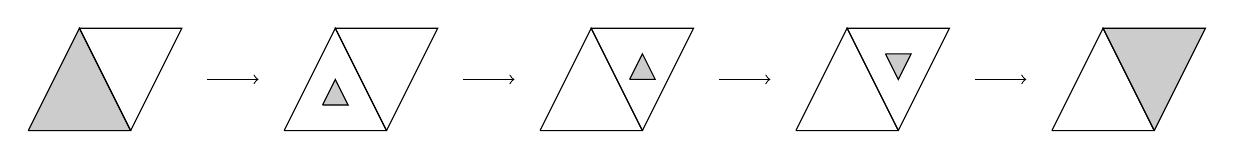
\begin{tikzpicture}[scale=0.65]
\draw[fill=black,opacity=0.2] (0,0) -- (2,0) -- (1,2) -- (0,0);
\draw (0,0) -- (2,0) -- (1,2) -- (0,0);
\draw(2,0) -- (3,2) -- (1,2) -- (2,0);

\draw[->] (3.5,1) -- (4.5,1);

\draw[fill=black,opacity=0.2] (5.75,0.5) -- (6.25,0.5) -- (6,1) -- (5.75,0.5);
\draw (5.75,0.5) -- (6.25,0.5) -- (6,1) -- (5.75,0.5);
\draw (5,0) -- (7,0) -- (6,2) -- (5,0);
\draw(7,0) -- (8,2) -- (6,2) -- (7,0);

\draw[->] (8.5,1) -- (9.5,1);

\draw (10,0) -- (12,0) -- (11,2) -- (10,0);
\draw(12,0) -- (13,2) -- (11,2) -- (12,0);
\draw (11.75,1) -- (12.25,1) -- (12,1.5) -- (11.75,1);
\draw[fill=black,opacity=0.2] (11.75,1) -- (12.25,1) -- (12,1.5) -- (11.75,1);

\draw[->] (13.5,1) -- (14.5,1);

\draw (15,0) -- (17,0) -- (16,2) -- (15,0);
\draw (17,0) -- (18,2) -- (16,2) -- (17,0);
\draw (16.75,1.5) -- (17.25,1.5) -- (17,1) -- (16.75,1.5);
\draw[fill=black, opacity=0.2] (16.75,1.5) -- (17.25,1.5) -- (17,1) -- (16.75,1.5);

\draw[->] (18.5,1) -- (19.5,1);

\draw (20,0) -- (22,0) -- (21,2) -- (20,0);
\draw (22,0) -- (23,2) -- (21,2) -- (22,0);
\draw[fill=black,opacity =0.2] (22,0) -- (23,2) -- (21,2) -- (22,0);

\end{tikzpicture}
$$
where the dark triangle denotes a special simplex, the white one an ordinary simplex, we can form "special pairs" ($\sigma_+, \sigma_-)$ sharing precisely one face which maps to $\tau$ by "mirror images". Indeed consider $g_{\sigma_+}$. As explained, we can move $g_{\sigma_-}$ to the domain of $g_{\sigma_+}$. Thus, by simplicity, there exists an automorphism $a \in \Delta^n \cong S_{n+1}$, such that $g_{\sigma_-} \sim g_{\sigma_+} \circ \overline{s}$ with 
$$
\begin{xy}
\xymatrix{
\Delta^n \ar[rr]^{s} \ar[d] && \Delta^n \ar[d] \\
\slant{\Delta^n}{\partial \Delta^n} \ar[rr]_{\overline{s}} && \slant{\Delta^n}{\partial \Delta^n}
}
\end{xy}
$$
Now every element in the symmetric group is generated of transpositions $\tau_i$; i.e. we obtain
$$\deg g_{\sigma_-} = \deg g_{\sigma_+} \ \deg \overline{s} = \deg g_{\sigma_+} \ \deg \prod_{i=1}^r \tau_i = \deg g_{\sigma_+} (-1)^r = \deg g_{\sigma_+} \mathrm{sgn}(s).$$
By continuously rotating the reflection hyperplane to any face of the simplex we can form a special pair mapped to $\tau$ by mirror images.
Embedding $\sigma_+ \cup \sigma_-$ into $\mathbb{R}^{n+1}$ as indicated

$$
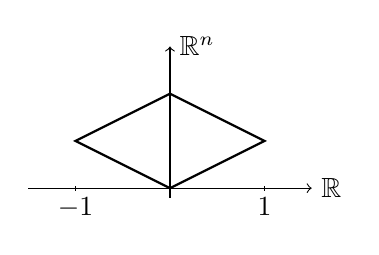
\begin{tikzpicture}[scale=0.6]

\draw[thin,->] (-3,0) -- (3,0);
\draw[thin, ->] (0,-0.2) -- (0,3);
\draw[thick] (0,0) -- (-2,1) -- (0,2) -- (2,1) -- (0,0);
\draw (0,3) node[right] {$\mathbb{R}^n$};
\draw (3,0) node[right] {$\mathbb{R}$};
\draw (2,0) node[below] {$1$};
\draw (-2,0) node[below] {$-1$};
\draw (-2,-0.05) -- (-2,0.05);
\draw (2,-0.05) -- (2,0.05);

\end{tikzpicture}
$$
we can extend $g \vert_{\sigma_+ \cup \sigma_-}$ to $h: \mathbb{R}^{n+1} \la K$ by setting $h\equiv v$ outside $\sigma_+ \cup \sigma_-$. Then $h(x,y) = h(-x,y)$. The homotopy
$$F(x,y,t) = \begin{cases} \ h(x,y), & \textrm{ if } \vert x \vert \geqslant t \\ \ h(t,y), & \textrm{ if } \vert x \vert \leqslant t \end{cases} $$
turns $\sigma_+$ and $\sigma_-$ into ordinary simplices. $\hfill \Box$

\end{pr}


\end{lemma}


\begin{remark}
The formula $\deg g = \sum \deg g_{\sigma}$ in the proof of the preceeding lemma has a differential-topological interpretation: Let $f: \Sph^n \la \Sph^n$ be smooth and $q \in \Sph^n$ a regular value with $f^{-1}(q) = \{p_1, \ldots, p_k\}$. Then 
$$\deg f = \sum_{l=1}^k \mathrm{sgn} \ \det \left( \frac{\partial f_i}{\partial x_j} (p_l) \right).$$

\end{remark}

\begin{theorem}
The map 
$$ \deg: \langle \Sph^n, \Sph^n \rangle \la \Z, \qquad [f]\mapsto \deg f$$
is an isomorphism of groups. 
\begin{pr}
We first show that $\deg$ is a homomorphism. For $[f], [g] \in \langle \Sph^n, \Sph^n\rangle = \pi_n(\Sph^n, \star)$ factors as
$$
\begin{xy}
\xymatrix{
\tilde{H}_n(\Sph^n) \ar[rrr] \ar[rrrd]_{z \mapsto (z,z)} &&& \tilde{H}_n(\Sph^n \vee \Sph^n) \ar[d]^{\sim} \ar[rrr]^{\tilde{H}_n(f \vee g)} &&& \tilde{H}_n(\Sph^n) \\ &&& \tilde{H}_n(\Sph^n) \oplus \tilde{H}_n(\Sph^n) \ar[rrru]_{\qquad \qquad \qquad (z_1, z_2) \mapsto \tilde{H}_n(f)(z_1) + \tilde{H}_n(g)(z_2)} &&&
}
\end{xy}
$$
We then obtain $\deg f \star g = \deg f + \deg g$. Surjectivity is easy: $\id_{\Sph^1}$ maps to $1$ and since $1$ generates $\Z$, $\deg$ is surjective. Injectivity follows from lemma 4.7, which finishes the proof. $\hfill \Box$
\end{pr}

\end{theorem}


\begin{corollary}
The map $[\Sph^n, \Sph^n] \la \Z$ is a bijection independant of the homology theory $(H_*, \partial_*)$.
\begin{pr}
Given $f: \Sph^n \la \Sph^n$, a great arc from some $x_0 \in \Sph^n$ to $f(x_0)$ is a contractible CNDR and therefore $f \sim \overline{f}$ where $\overline{f}(x_0) = x_0$. Then the inclusion induces a bijection $\langle\Sph^n, \Sph^n\rangle \la [\Sph^n, \Sph^n]$, i.e. $\deg$ is bijective. Thus the maps $\sum_{i=1}^{n-1} f_k  = S^{n-1} f_k$ form a system of representatives of $[\Sph^n, \Sph^n]$ and as we saw above, $\deg S^{n-1}f_k = \deg f_k = k$ is independant of $(H_*, \partial_*)$. $\hfill \Box$

\end{pr}

\end{corollary}





























\section{Applications} %PARAGRAPH V.5




In this section let $(H_*, \partial_*)$ be a homology theory with values in $\Z$ which satisfies the dimension axiom (e.g. $(\Hs_*, \partial^{\mathrm{sing}}_*)$).

\begin{theorem}[fundamental theorem of algebra]
Let $p(z) = z^n + a_{n-1}z^{n-1} + \ldots + a_1z + a_0$ with coefficients $a_i \in \mathbb{C}$ and $n \geqslant 1$. Then $p$ has a zero in $\mathbb{C}$. 
\begin{pr}
Assume $p(z)\neq 0$ for all $z \in \mathbb{C}$. Then 
$$f_t(z) := \frac{ p(tz)}{\Vert p(tz)\Vert}$$
for $z \in \mathbb{C}$ and $t \in \mathbb{R}$ defines a nullhomotopic map $f_t: \Sph^1 \la \Sph^1$, i.e. $\deg f_t = 0$. Chosse $r_0 \gg 0$ so large that for $ z \in \mathbb{C}$ with $\vert z \vert = r_0$ we have
$$\vert z \vert^n > \vert a_{n-1} z^{n-1} + \ldots + a_1 z + a_0 \vert.$$
Let $p_t(z) := z^n + t (a_{n-1}z^{n-1} + \ldots + a_1z + a_0)$ and 
$$g_t: \Sph^1 \la \Sph^1, \qquad g_t(z) = \frac{p_t(r_0z)}{\Vert p_t(r_0 z)\Vert}$$
Then it follows $f_{r_0} =g_1 \sim g_0$, i.e. 
$$0 = \deg f_{r_0} = \deg g_0 = \deg (z \mapsto z^n) = n \geqslant 1,$$
a contradcition. $\hfill \Box$

\end{pr}

\end{theorem}



\begin{theorem}[Invariance of domain]
For $m,n \in \mathbb{N}_0$ we have $\mathbb{R}^m \cong \mathbb{R}^n$ if and only if $n=m$.
\begin{pr}
Clearly $\mathbb{R}^n \cong \mathbb{R}^m$ if $m=n$. For the converse consider a homeomorphism $f: \mathbb{R}^n \la \mathbb{R}^m$. Then
$$\Sph^{n-1} \sim \mathbb{R}^n \setminus \{0\} \cong \mathbb{R}^m \setminus \{ f(0)\} \sim \Sph^{m-1},$$
i.e. 
$$\Z = \tilde{H}_{n-1}(\Sph^{n-1}) \cong \tilde{H}_{n-1}(\Sph^{m-1}) \cong \begin{cases} \ \Z, & \textrm{ if } m-1=n-1 \\ \ 0, & \textrm{ otherwise} \end{cases},$$
i.e. $m=n$. $\hfill \Box$
\end{pr}

\end{theorem}


\begin{theorem}[nonexistence of retractions]
The $n$-disc $\mathbb{D}^n$ does not retract onto $\Sph^{n-1}$.
\begin{pr}
Let $r: \mathbb{D}^n \la \Sph^{n-1}$ be retraction, i.e. $r\vert_{\Sph^{n-1}} = \id_{\Sph^{n-1}}$. Then the composition
$$\Sph^{n-1} \overset{\id}{\la} \mathbb{D}^n \overset{r}{\la} \Sph^{n-1}$$
is the identity on $\mathbb{S}^{n-1}$. However in homology we have
$$\tilde{H}_{n-1}(\mathbb{S}^{n-1}) = \mathbb{Z} \xrightarrow{\tilde{H}_{n-1}(\id)} 0 = \tilde{H}_{n-1}(\mathbb{D}^n) \xrightarrow{\tilde{H}_{n-1}(r)} \mathbb{Z}$$
which clearly is the zero map, a contradicition. $\hfill \Box$



\end{pr}
\end{theorem}


\begin{theorem}[Brouwer's fix point theorem]
Every continuous map $f: \mathbb{D}^n \la \mathbb{D}^n$ has a fixed point.
\begin{pr}
For $n=0$ nothing is to prove. Assume $n\geqslant 1$. Suppose $f(x) \neq x$ for all $x \in \mathbb{D}^n$. Then let 
$r: \mathbb{D}^n \la \Sph^n$ be the map, which assigns to any $x \in \mathbb{D}^n$ the unique intersection point of the ray from $f(x)$ through $x$ and $\Sph^{n-1}$. Then clearly $r$ is continuous and $r\vert_{\Sph^{n-1}} = \id_{\Sph^{n-1}}$, i.e. $r$ is a contraction which contradicts theorem 5.3. $\hfill \Box$

\end{pr}
\end{theorem}


The next application is intrinsic to singular homology; thus let $(H_*, \partial_*) = (\Hs_*, \partial^{\mathrm{sing}}_*)$ and $C_*=\Cs_*$.


\begin{theorem}[Borsuk-Ulam-theorem]
For every continuous map $f: \Sph^n \la \mathbb{R}^{n}$ there is a point $x \in \Sph^n$ such that $f(x) = f(-x)$.
\end{theorem}


\begin{theorem}[Ham-Sandwich-theorem]
Let $A_1, \ldots, A_m \subseteq \mathbb{R}^m$ be Borel sets of finite Lebesgue measure $\lambda(A_i) < \infty$. Then there is an affine hyperplane in $\mathbb{R}^m$ which disects each $A_i$ into equal measure subsets. 
\begin{pr}
Consider the affine subspace $\mathbb{R}^m \times \{1\} \subseteq \mathbb{R}^{m+1}$. Given any $x \in \mathbb{R}^{m+1} \setminus \{0\}$, set
$$H_x^+ := \{ y \in \mathbb{R}^{m+1} \ \vert \ \langle x,y\rangle \geqslant 0 \} \cap \mathbb{R}^m \times \{1\}$$
$$H_x^- := \{ y \in \mathbb{R}^{m+1} \ \vert \ \langle x,y\rangle \leqslant 0 \} \cap \mathbb{R}^m \times \{1\}$$
$$H_x:= H_x^+ \cap H_x^-.$$
For $i \in \{1,\ldots, m\}$ let further 
$$f_i: \Sph^m \la \mathbb{R}, \qquad x  \mapsto \lambda \left( A_i \cap H_x^+\right)$$
where again $\lambda$ denotes the Lebesgue measure. Then $f_i(x) = \lambda(A_i \cap H_{-x}^+) = \lambda(A_i \cap H_x^-)$. Now define
$$f: \Sph^m \la \mathbb{R}^m, \qquad x \mapsto (f_1(x), \ldots, f_m(x)).$$
We now show that $f$ is continuous. Let $(x_n)_{n \in \mathbb{N}}$ be any sequence in $\Sph^m$ converging to $x \in \Sph^m$. We have to show, that the sequence of images $(f(x_n))_{n \in \mathbb{N}}$ converges to $f(x)$. Let $\chi$ denote the indicator function. Then
$$\chi_{A_i \cap H_{x_n}^{\pm}} \xrightarrow{\mathrm{pointwise}} \chi_{A_i \cap H_x^{\pm}}$$
except (possibly) on $A_i \cap H_x$, which is null, i.e. the above holds $\lambda$-almost everywhere. But then by the theorem of dominated convergence we have
$$f_i(x_n) = \int \chi_{A_i \cap H_{x_n}^{\pm}} \ \mathrm{d} \lambda \xrightarrow{n \to \infty} \int \chi_{A_i \cap H_x^{\pm}} \ \mathrm{d}\lambda = f_i(x)$$
for all $i \in \{1, \ldots, m\}$, i.e. $f(x_n) \xrightarrow{n \to \infty} f(x)$. 
Now by theorem 5.5, there exists some $\tilde{x} \in \Sph^m$, such that $f(\tilde{x})=f(-\tilde{x})$, i.e.
$$\lambda(A_i \cap  H_{\tilde{x}}^+) = f_i(\tilde{x}) = f_i(-\tilde{x}) = \lambda(A_i \cap H_{\tilde{x}}^-)$$
for all $i \in \{1,\ldots, m\}$, which means that the hyperplane $H_{\tilde{x}}$ divides all the $A_i$'s into two equal measure subsets. $\hfill \Box$
\end{pr}
\end{theorem}



\begin{theorem}[Equivariance / antipode theorem]
Let $g: \Sph^n \la \Sph^m$ continuous with $g(-x) = -g(x)$ for all $x \in \Sph^n$. Then $n \leqslant m$.
\end{theorem}

\begin{pr}
The group $\langle t \vert t^2 \rangle \cong \slant{\Z}{2 \Z}$ acts on $\Sph^k$ by $t \cdot x := -x$ and $\slant{\Sph^k}{\slant{\Z}{2\Z}} \cong \mathbb{P}^k(\mathbb{R})$ and we obtain that $p: \Sph^k \la \mathbb{P}^k(\mathbb{R})$ is a two-sheeted covering space. Covering theory says: For each singular $p$-simplex $\sigma: \Delta^p \la \mathbb{P}^k(\mathbb{R})$ there are precisle two lifts $\overline{\sigma}_+$ and $\overline{\sigma}_-$ fitting into the diagram

$$
\begin{xy}
\xymatrix{
& ( \Sph^k, \star) \ar[rd]  & \\ (\Delta^p,0) \ar[ru]_{\overline{\sigma}_+}^{\overline{\sigma}_-} \ar[rr]_{\sigma} && (\mathbb{P}^k(\mathbb{R}), \star) 
}
\end{xy}
$$
 
 which are swapped by $t$, i.e. $t \cdot \overline{\sigma}_{\pm} = \overline{\sigma}_{\mp}$. We obtain the chain map
 $$
 \tau_* : C_*\left( \mathbb{P}^k(\mathbb{R}), \slant{\Z}{2 \Z}\right) \la C_*\left( \Sph^k, \slant{\Z}{2 \Z} \right), \qquad \sigma \mapsto \overline{\sigma}_+ + \overline{\sigma}_-,$$
 called the ***. $\tau_*$ gives rise to a short exact sequence
 $$0 \la C_*\left( \mathbb{P}^k(\mathbb{R}), \slant{\Z}{2 \Z}\right) \overset{\tau_*}{\la} C_*\left( \Sph^k, \slant{\Z}{2 \Z} \right) \overset{C_*(p)}{\la} C_*\left( \mathbb{P}^k(\mathbb{R}), \slant{\Z}{2 \Z}\right) \la 0$$
 Now let $g: \Sph^n \la \Sph^m$ be an equivariant map, i.e. $g(x) = -g(-x)$ for all $x \in \Sph^n$. Then $g$ induces $\overline{g}: \mathbb{P}^n(\mathbb{R}) \la \mathbb{P}^m(\mathbb{R})$. We obtain a diagram
 $$
 \begin{xy}
 \xymatrix{
 0 \ar[r] & C_*\left( \mathbb{P}^n(\mathbb{R}), \slant{\Z}{2 \Z}\right) \ar[d]_{C_*(\overline{g})} \ar[r] & C_*\left( \Sph^n, \slant{\Z}{2\Z} \right) \ar[d]_{C_*(g)} \ar[r] & C_*\left( \mathbb{P}^n(\mathbb{R}), \slant{\Z}{2 \Z}\right) \ar[d]_{C_*(\overline{g})} \ar[r] & 0 \\
 0 \ar[r] & C_*\left( \mathbb{P}^m(\mathbb{R}), \slant{\Z}{2 \Z}\right) \ar[r] & C_*\left(\Sph^m, \slant{\Z}{2\Z}\right) \ar[r] & C_*\left( \mathbb{P}^m(\mathbb{R}), \slant{\Z}{2 \Z}\right) \ar[r] & 0
 }
 \end{xy}
 $$

and hence a commuting ladder of long exact sequences. Indded, for commutativity of 
$$
\begin{xy}
\xymatrix{
C_*\left(\mathbb{P}^n(\mathbb{R}), \slant{\Z}{2\Z} \right) \ar[r]^{\tau_*} \ar[d]_{c_*(\overline{g})} & C_*\left(\mathbb{S}^n, \slant{\Z}{2\Z} \right) \ar[d]_{c_*(g)} \\ C_*\left(\mathbb{P}^m(\mathbb{R}), \slant{\Z}{2\Z} \right) \ar[r]^{\tau_*} & C_*\left(\mathbb{S}^m, \slant{\Z}{2\Z} \right)
}
\end{xy}
$$
consider the diagram
$$
\begin{xy}
\xymatrix{
\mathbb{P}^n(\mathbb{R}) \ar[d]_{\overline{g}} & \mathbb{S}^n \ar[l]_{p_n} \ar[d]_g \\ \mathbb{P}^m(\mathbb{R}) & \mathbb{S}^m \ar[l]_{p_m}
}
\end{xy}
$$
Let $\sigma: \Delta_p: \mathbb{P}^n(\mathbb{R})$ and let $\overline{\sigma}_{\pm}$ be the unique two lifts of $\sigma$ under $p_n$. Then we obtain 
$$p_m \circ \overline{\sigma}_{\pm} = (p_m \circ g) \circ \overline{\sigma}_{\pm} = (\overline{g} \circ p_n) \circ \overline{\sigma}_{\pm} = \overline{g} \circ (p_n \circ \overline{\sigma}_{\pm}) = \overline{g} \circ \sigma,$$
thus $g \circ \overline{\sigma}_{\pm}$ are the two unique lift of $\overline{g} \circ \sigma$ under $p_m$. \\
Now we know that $\mathbb{P}^m(\mathbb{R})$ has an $m$-dimensional $\Delta$-structure, i.e. 
$$H_{n-1}\left(\mathbb{P}^m(\mathbb{R}), \slant{\Z}{2\Z}\right) = 0.$$
Thus the corresponding long exact sequence
$$
\begin{xy}
\xymatrix{
 \ldots \ar[r] & 0 \ar[r] & H_m\left( \mathbb{P}^m(\mathbb{R}), \slant{\Z}{2 \Z} \right) \ar[r]^{H_m(\tau_*)} & H_m\left( \Sph^m, \slant{\Z}{2\Z}\right) \ar[r]^{H_m(p)} & H_m\left( \mathbb{P}^m(\mathbb{R}), \slant{\Z}{2 \Z} \right) & \\
 & \ar[r] & H_{m-1}\left( \mathbb{P}^m(\mathbb{R}), \slant{\Z}{2 \Z} \right) \ar[r] & H_{m-1}\left( \Sph^m, \slant{\Z}{2\Z}\right) \ar[r] & H_{m-1}\left( \mathbb{P}^m(\mathbb{R}), \slant{\Z}{2 \Z} \right)& \\
 & \ar[r] & H_{m-1}\left( \mathbb{P}^m(\mathbb{R}), \slant{\Z}{2 \Z} \right) \ar[r] & \ldots \qquad \qquad \qquad  && \\
  & \ar[r] & H_{1}\left( \mathbb{P}^m(\mathbb{R}), \slant{\Z}{2 \Z} \right) \ar[r] & H_{1}\left( \Sph^m, \slant{\Z}{2\Z}\right) \ar[r] & H_{1}\left( \mathbb{P}^m(\mathbb{R}), \slant{\Z}{2 \Z} \right)& \\
 & \ar[r] & H_{0}\left( \mathbb{P}^m(\mathbb{R}), \slant{\Z}{2 \Z} \right) \ar[r] & H_{0}\left( \Sph^m, \slant{\Z}{2\Z}\right) \ar[r] & H_{0}\left( \mathbb{P}^m(\mathbb{R}), \slant{\Z}{2 \Z} \right) \ar[r] & 0 \\
}
\end{xy}
$$
becomes to 

$$
\begin{xy}
\xymatrix{
 \ldots \ar[r] & 0 \ar[r] & H_m\left( \mathbb{P}^m(\mathbb{R}), \slant{\Z}{2 \Z} \right) \ar[r]^{\qquad H_m(\tau_*)} & \slant{\Z}{2\Z} \ar[r]^{H_m(p) \qquad } & H_m\left( \mathbb{P}^m(\mathbb{R}), \slant{\Z}{2 \Z} \right) & \\
 & \ar[r]^{\sim \qquad \qquad } & H_{m-1}\left( \mathbb{P}^m(\mathbb{R}), \slant{\Z}{2 \Z} \right) \ar[r]^{0} & 0 \ar[r] & H_{m-1}\left( \mathbb{P}^m(\mathbb{R}), \slant{\Z}{2 \Z} \right)& \\
 & \ar[r]^{\sim \qquad \qquad  } & H_{m-1}\left( \mathbb{P}^m(\mathbb{R}), \slant{\Z}{2 \Z} \right) \ar[r] & \ldots \qquad \qquad \qquad  && \\
  & \ar[r]^{\sim \qquad \qquad } & H_{1}\left( \mathbb{P}^m(\mathbb{R}), \slant{\Z}{2 \Z} \right) \ar[r] & 0 \ar[r] & H_{1}\left( \mathbb{P}^m(\mathbb{R}), \slant{\Z}{2 \Z} \right)& \\
 & \ar[r]^{\sim} &  \slant{\Z}{2 \Z} \ar[r]^{0} &  \slant{\Z}{2\Z} \ar[r]^{\sim} & \slant{\Z}{2 \Z} \ar[r] & 0 \\
}
\end{xy}
$$
i.e. the boundaries are isomorphisms. Note that 
$$H_m(\tau_*) \circ H_m(p) = i_{H_m(\Sph^n)} + H_m\left( \Sph^m \overset{t}{\la} \Sph^m, \ x \mapsto -x \right) = \id_{H_m(\Sph^m)} \pm \id_{H_m(\Sph^m)} = 0$$
und thus the long exact sequence gives us $H_m(p) \circ H_m(\tau_*) =0$.
Since $H_m(\tau_*)$ is injective, we have that $H_m(p)=0$. Thus for $n \geqslant m$ and $1 \leqslant i \leqslant m$ we obtain a commuting square
$$
\begin{xy}
\xymatrix{
H_i\left( \mathbb{P}^n(\mathbb{R}), \slant{\Z}{2 \Z} \right) \ar[d]_{H_i(\overline{g})} \ar[r]^{\partial}_{\cong} & H_{i-1}\left( \mathbb{P}^n(\mathbb{R}), \slant{\Z}{2\Z}\right) \ar[d] \\ H_i\left( \mathbb{P}^m(\mathbb{R}), \slant{\Z}{2 \Z} \right) \ar[r]^{\cong}_{\partial} & H_i\left( \mathbb{P}^m(\mathbb{R}), \slant{\Z}{2 \Z} \right)
}
\end{xy}
$$
Since $H_0(\overline{g})$ is an isomorphism, so is $H_i(\overline{g})$ for $1 \leqslant i \leqslant m$. Now assume $n>m$. Then we have 
$$
\begin{xy}
\xymatrix{
H_m\left( \mathbb{P}^n(\mathbb{R}), \slant{\Z}{2 \Z} \right) \ar[d]_{H_m(\overline{g})}^{\cong} \ar[r]^{H_m(\tau_*)} & H_{m}\left( \Sph^m, \slant{\Z}{2\Z}\right) = 0 \ar[d]_{H_m(g)} \\ H_m\left( \mathbb{P}^m(\mathbb{R}), \slant{\Z}{2 \Z} \right) \ar[r]^{\cong}_{H_m(\tau_*)} & H_m\left( \Sph^m, \slant{\Z}{2 \Z} \right) \cong \slant{\Z}{2\Z}
}
\end{xy}
$$

which means that the isomorphism $H_m(\tau_*) \circ H_m(\overline{g})$ factors over $0$ - which is impossible. Thus $n \leqslant m$, which finishes the proof. $\hfill \Box$


\end{pr}









\begin{pr}[\textrm{\textit{proof of theorem 5.5}}]
Assume $f$ satisifes $f(x) \neq f(-x)$ for all $x \in \Sph^n$.Then the map 
$$g: \Sph^n \la \Sph^{n-1}, \qquad x \mapsto \frac{f(x)- f(-x)}{\Vert f(x) - f(-x)\Vert}$$
is continuous and satisfies $g(x) = -g(-x)$ for all $x \in \Sph^n$, which contradicts theorem 5.7. $\hfill \Box$
\end{pr}
































































\chapter{Cell complexes and cellular homology} %KAPITEL VI
\setlength\abovedisplayshortskip{0pt}
\setlength\belowdisplayshortskip{10pt}
\setlength\abovedisplayskip{10pt}
\setlength\belowdisplayskip{10pt}





\section{CW-complexes} %PARAGRAPH VI.1

\thispagestyle{empty}

\begin{defin}
A \textit{CW-complex} is a topological space $X$ together with a filtration $\emptyset = X_{-1} \subseteq X_0 \subseteq X_1 \subseteq \ldots$ of subspaces $X_i \subseteq X$ for $i \geqslant -1$, such that
\begin{compactenum}
\item For all $n \geqslant 0$ there exist pushout diagrams in $\topsp$:
$$
\begin{xy}
\xymatrix{
\coprod_{i \in I^n} \mathbb{S}^{n-1} \ar[rr]^{\amalg_{i \in I^n} q_i^n} \ar[d]_{\amalg_{i \in I^n} \iota} && X_{n-1} \ar[d] \\ \coprod_{i \in I^n} \mathbb{D}^n \ar[rr]^{\amalg_{i \in I^n} Q_i^n} && X_n
}
\end{xy}
$$
\item We have $X= \mathrm{colim} \ X_n$ in $\topsp$. 
\end{compactenum}

\end{defin}


\begin{expl}
\begin{compactenum}
\item Since $\mathbb{D}^0=\{ \cdot\}$, for $n=0$ the first condition gives us the existence of a pushout
$$
\begin{xy}
\xymatrix{
\emptyset \ar[d] \ar[r] & \emptyset \ar[d] \\ \coprod_{ i \in I^n} \{\cdot \} \ar[r]^{\cong} & X_0
}
\end{xy}
$$
Thus $X_0$ is a discrete subset of $X$.

\item For $n\geqslant 1$, the first condition says, that the $n$-skeleton $X_n$ of $X$ is obtained from the $n-1$-skeleton by attaching $n$-dimensional cells $Q_i^n(\mathbb{d}^n)$ along the attaching maps $q_i^n: \mathbb{S}^n \la X_{n-1}$. $Q_i^n$ is called the \textit{characteristic map} of the cell.

\item The second condition says that
$$X= \bigcup_{n \geqslant -1} X_n$$
as a set and that $X$ carries the \textit{final topology} with respect to the inclusions $X_{n-1} \hookrightarrow X_n$, i.e. a subset $D\subseteq X$ is closed in $X$ if and only if for all $n \geqslant 1$ the intersections $D \cap X_n \subseteq X_n$ are closed. Indeed, this is the maximal choice of closed sets, such that $X$ still is a cocone in $\topsp$:
$$
\begin{xy}
\xymatrix{
X_{n-1} \ar[rr] \ar[rd]_{i_{n-1}} && X_n \ar[ld]^{i_n} \\ & X & 
}
\end{xy}
$$
More precisely, if $D \subseteq X$ is closed but $D \cap X_n$ for some $n \geqslant -1$ is not, that $i_n$ is no longer continuous. Now on the other hand, universailty of the cocone above requires that $X$ has no less closed subsets. Assume $X'$ to be the set $X$ carrying a coarser topology than $X$. Then the identity $\id: X' \la X$ is no longer continous, violating the universal property:
$$
\begin{xy}
\xymatrix{
X_{n-1} \ar[rr] \ar[rd]_{i'_{n-1}} \ar@/_{20pt}/[rdd]_{i_{n-1}} && X_n \ar[ld]^{i_n'}  \ar@/^{20pt}/[ldd]^{i_n} \\
& X' \ar@{-->}[d]^{\mathrm{\exists ! id}} & \\ & X &
}
\end{xy}
$$

\item The filtration is part of the structure of a CW-complex, while the pushouts are not. Only the existence of pushouts is required.

\end{compactenum}

\end{expl}



\begin{defin}
Replacing $X_{-1} = \emptyset$ with $X_{-1} :=A$ for some Hausdorff subset $A\subseteq X$ in the definition of a CW-complex gives us the definition of a \textit{relative CW-complex} $(X,A)$.
\end{defin}

\begin{defin}
Let $(X,A)$, $(Y,B)$ be relative CW-complexes and $f: (X,A) \la (Y,B)$ a map of pairs. Then $F$ is called \textit{cellular}, if $f(X_n) \subseteq Y_n$ for all $n \geqslant -1$. This gives us categories $\CW$ and $\redCW$. Analogously we find $\CWtwo$ the category of pairs of CW-complexes.

\end{defin}




\begin{defin}
Let $(X,A)$ be a relative CW-complex. Then the \textit{dimension} of $(X,A)$ is $\dim (X,A) = n \geqslant -1$, if $X=X_n$. We say that $(X,A)$ is \textit{relatively finite}, if it has finitely many cells. Obviously (relatively) finite CW-complexes are of finite dimension but the converse is not true.

\end{defin}


\begin{ex}
\begin{compactenum}
\item  Let $X= \mathbb{S}^{n}$ and $x \in \Sph^n$, $X_{i-1} = \emptyset$, $X_0=X_1=\ldots = X_{n-1} = \{ x\}$ and $X_n= \mathbb{S}^n$. With this filtration, then $n$-sphere becomes a CW-complex. For $k \in \{1, \ldots, n-1\}$ we have pushout diagrams
$$
\begin{xy}
\xymatrix{
\emptyset \ar[r] \ar[d] & X_{k-1} \ar[d] \\ \emptyset \ar[r] & X_k 
}
\end{xy}
$$
(note that $I^k=\emptyset$ for these $k$) and for $k=n$ we have our well-known diagram
$$
\begin{xy}
\xymatrix{
\mathbb{S}^{n-1} \ar[r] \ar[d] & \{ x\} = X_{n-1} \ar[d] \\ \mathbb{D}^n \ar[r] & \mathbb{S}^n =X_n
}
\end{xy}
$$

\item Let $F_g$ be a surface of genus $g$, $x \in F_g$ and choose a filtration $X_{-1} = \emptyset$, $X_0=\{ x\}$, $X_1 = \bigvee_{i=1}^{2g} \mathbb{S}^1$, $X_2=X$. Then we have the three pushout diagrams for $k=0$:
$$
\begin{xy}
\xymatrix{
\mathbb{S}^{-1} = \emptyset \ar[r] \ar[d] & \emptyset =  X_{-1} \ar[d] \\  \mathbb{D}^0 = \{x\} \ar[r] & \{ x\} = X_0
}
\end{xy}
$$
for $k=1$:
$$
\begin{xy}
\xymatrix{
\coprod_{i =1}^{2g} \mathbb{S}^0 \ar[d] \ar[r] & \{x\} \ar[d] \\ \coprod_{i=1}^{2g} \mathbb{D}^1 \ar[r] & \bigvee_{i=1}^{2g} \mathbb{S}^1
}
\end{xy}
$$
and for $k=2$:
$$
\begin{xy}
\xymatrix{
\mathbb{S}^1 \ar[d] \ar[r]^{q^2} & \bigvee_{i=1}^{2g} \mathbb{S}^1 \ar[d] \\ \mathbb{D}^2 \ar[r] & X
}
\end{xy}
$$
where $[q^2] \in \pi_1(X_1)= F(a_1,b_1, \ldots, a_g,b_g)$ is the surface word $\prod_{i=1}^g [a_ib_i]$.

\item Let $X= \mathbb{P}^d(\mathbb{R})$, $X_{-1}= \emptyset$ and for $n\in \{0, \ldots, d\}$
$$X_n:= \{ (x_0: \ldots: x_n:0 \ldots : 0 ) \ \vert \ x_i \in \mathbb{R} \textrm{ for } i \in \{0, \ldots, n\} \} \cong \mathbb{P}^n(\mathbb{R}).$$
Then $X$ together with this filtration is a CW-complex. Consider the pushouts for $n \in \{0, \ldots, d \}$
$$
\begin{xy}
\xymatrix{
\mathbb{S}^{n-1} \ar[d] \ar[r]^{q^n\qquad  \ } & \mathbb{P}^{n-1}(\mathbb{R}) = X_{n-1} \ar[d] \\ \mathbb{D}^n \ar[r]^{Q^n \qquad } & \mathbb{P}^n(\mathbb{R}) = X_n
}
\end{xy}
$$
with the $2$-fold covering
$$q^n: \mathbb{S}^{n-1} \la \mathbb{P}^{n-1} (\mathbb{R}), \qquad (x_1, \ldots, x_n) \mapsto (x_1: \ldots : x_n)$$
and $Q^n= q^{n+1} \circ s_n$ with the reversed stereographic projection 
$$s_n: \mathbb{D}^n \la \mathbb{S}^{n}, \qquad (x_1, \ldots, x_n) \mapsto \left(x_1, \ldots, x_n, \sqrt{1- \Vert (x_1, \ldots, x_n) \Vert^2 } \right)$$


\item Now consider the complex projective space $X= \mathbb{P}^{d}(\mathbb{C})$ with the filtration
$$X_{2n} = X_{2n+1} := \{ (z_1: \ldots : z_n:0: \ldots : 0 ) \ \vert z_i \in \mathbb{C} \textrm{ for } i \in i \in \{0, \ldots, n \} \} \cong \mathbb{P}^n(\mathbb{C})$$
Then by the same pushout
$$
\begin{xy}
\xymatrix{
\mathbb{S}^{2n-1} \ar[d] \ar[r]^{q^{2n} \qquad\ \  } & \mathbb{P}^{n-1}(\mathbb{C}) = X_{2n-1} \ar[d] \\ \mathbb{D}^{2n} \ar[r]^{Q^{2n}\qquad} & \mathbb{P}^{2n}(\mathbb{C}) = X_{2n} 
}
\end{xy}
$$
where again 
$$q^{2n}(z_1, \ldots, z_n) = \left( z_1:\ldots: z_n:0:\ldots:0\right)$$
$$Q^{2n}(z_1, \ldots, z_n) = \left( z_1: \ldots: z_n : \sqrt{1- \Vert (z_1, \ldots z_n) \Vert^2}\right)$$

Note that for $n=2$, $q^{2n}=q^4: \mathbb{S}^3 \la \mathbb{P}^1(\mathbb{C}) \cong \mathbb{S}^2$ is the \textit{Hopf bundle}. It has the property $\pi_3(\mathbb{S}^2) = \langle [q^4]\rangle \cong \Z$, i.e. the homotopy class of the Hopf bundle generates the third homotopy group of the Riemann sphere and has infinite order. 

\end{compactenum}
\end{ex}

If $X$ and $Y$ are CW-complexes then clearly so is $X \amalg Y$. For the product an additional condition is necessary:





\begin{theorem}
Suppose $X,Y$ are CW-complexes and $X$ or $Y$ locally compact. Then $X \times Y$ is a CW-complex with skeleton
$$(X \times Y)_n= \bigcup_{p+q=n} X_p \times Y_q$$

\begin{pr}
We only address the crucial point $\bigvee_{i=1}^{\infty} \mathbb{S}^1$. By definition
$$\left( \coprod_{n\geqslant 0} \coprod_{i \in I_X^n} \mathbb{D}^n\right) \xrightarrow{ \amalg_{n \geqslant 0} \amalg_{i \in  I_X^n} Q(X)_i^n} X$$
and 
$$\left( \coprod_{n\geqslant 0} \coprod_{i \in I_Y^n} \mathbb{D}^n\right) \xrightarrow{ \amalg_{n \geqslant 0} \amalg_{i\in  I_Y^n} Q(Y)_i^n} Y$$
are idenfications. We have to show, that the cartesian product is an idenfitcation as well. But since we have
$$\left( \coprod_{n,i} Q(X)_i^n \right) \times \left( \coprod_{n,i} Q(Y)_i^n \right) = \left( \left( \coprod_{n,i} Q(X)_i^n\right) \times \id_{\coprod_{n,i} \mathbb{D}^n} \right) \circ \left( \id_X \times \left( \coprod_{n,i} Q(Y)_i^n\right) \right)$$
Now the theorem follows from theorem II.4.1. $\hfill \Box$




\end{pr}


\end{theorem}


\begin{defin}
Let $X$ be a CW-complex. $A\subseteq X$ is called a \textit{sub-CW-complex} or just \textit{subcomplex} of $X$ if $A \subseteq X$ is a subspace and a CW-complex, such that for cells $Q: \mathbb{D}^n \la A$ in $A$ also $\mathbb{D}^n \overset{Q}{\la} A \hookrightarrow X$ are cells in $X$.
\end{defin}


\begin{remark}
If $X,Y$ are CW-complexes, $A \subseteq Y$ a subcomplex and
$$
\begin{xy}
\xymatrix{
A \ar[rr]^{f} \ar[d] && X \ar[d] \\ Y \ar[rr] && Z
}
\end{xy}
$$
a pushout square, then $Z$ is a CW-complex.
\end{remark}










\section{Cellular homology} %PARAGRAPH VI.2




Let $(H_*, \partial_*)$ be a homology theory with values in $\Rmod$.

\begin{defin}
Let $(X,A)$ be a relative CW-complex. Then the \textit{cellular chain complex} $C_*^{H_*}(X,A;R)$ \textit{associated with} $(H_*, \partial_*)$ is given by
$$C_n^{H_*}(X,A;R) := H_n(X_n,X_{n-1};R)$$
with differentials
$$c_n^{H_*}: C_n^{H_*}(X,A;R) \la C_{n-1}^{H_*}(X,A;R)$$
given by the boundary homomorphisms
$$\partial_n: H_n(X_n, X_{n-1};R) \la H_{n-1}(X_{n-1}, X_{n-2};R)$$
in the triple sequence of $(X_n, X_{n-1}, X_{n-2})$ (see theorem 5.1.3). Then 
$$H_*^{CW}(X,A;R) := H_n(C_*^{H_*}(X,A;R))$$
is called the \textit{cellular homology associated with} $(H_*, \partial_*)$.
\end{defin}


\begin{remark}
Note that $C_*^{H_*}(X,A;R)$ indeed is a chain complex. 
$$
\begin{xy}
\xymatrix@C=0.2em{
&&&H_{n-1}(X_{n-1}) \ar[rd]^{\alpha} &&&&& \\
\ldots \ar[rr] && H_n(X_n,X_{n-1}) \ar[rr]^{c_n^{H_*}} \ar[ru]_{\partial_1} && H_{n-1}(X_{n-1}, X_{n-2}) \ar[rd]_{\beta} \ar[rr]^{c_{n-1}^{H_*}} && H_{n-2}(X_{n-2}, X_{n-3}) \ar[rr] && \ldots \\
&&&&& H_{n-2}(X_{n-2}) \ar[ru]_{\partial_2} &&&
}
\end{xy}
$$
where $\partial_1$ comes from the long exact sequence of the pair $(X_n, X_{n-1})$, $\partial_2$ from $(X_{n-2}, X_{n-3})$ and $\alpha, \beta$ are part of the long exact sequence of $(X_{n-1}, X_{n-2})$. But $\beta \circ \alpha=0$, thus, since the diagram commutes, $c_{n-1}^{H_*} \circ c_{n}^{H_+} = 0$ and $C_*^{H_*}$ is a chain complex.

\end{remark}


\begin{theorem}
Suppose $(X,A)$ is a relative finite CW-complex and $(H_*, \partial_*)$ satisfies the dimension axiom. Then there are isomorphisms
$$H_n^{CW}(X,A;R) \overset{\cong}{\la} H_n(X,A;R)$$
for all $n \geqslant 0$ which are finite with respect to cellular maps.
\begin{pr}
Choose pushouts
$$
\begin{xy}
\xymatrix{
\coprod_{i \in I^n} \mathbb{S}^{n-1} \ar[d] \ar[rr]^{ \amalg_{i \in I^n} q_i^n} && X_{n-1} \ar[d] \\
\coprod_{i \in I^n} \ar[rr]^{\amalg_{i \in I^n} \mathbb{D}^n Q_i^n} && X_n
}
\end{xy}
$$
Then for $k \in \Z$ we have
\begin{alignat*}{5}
H_k(X_n, X_{n-1};R) = \tilde{H}_k\left( \slant{X_n}{X_{n-1}};R\right) \ \ &\cong&& \ \ \tilde{H}_k \left( \bigvee_{i \in I^n} \mathbb{S}^n;R\right) \\
&\cong && \ \ \bigoplus_{i \in I^n} \tilde{H}_k (\mathbb{S}^n;R) \\
&\cong&& \ \ \bigoplus_{i \in I^n} \tilde{H}_k\left( S^n \mathbb{S}^0;R\right)\\
&\cong&& \ \ \bigoplus_{i \in I^n} \tilde{H}_{k-n}(\mathbb{S}^0;R) \\
&\cong&& \ \ \bigoplus_{i \in I^n} H_{k-n}(\{\cdot\};R),
\end{alignat*}
thus the dimension axiom implies
$$H_{k}(X_n, X_{n-1};R) = \bigoplus_{i \in I^n} H_{k-n}(\{ \cdot \};R) \ \cong \ \begin{cases} \ \bigoplus_{i \in I^n} R, & \textrm{ if }k=n, \\ \ 0, & \textrm{ otherwise.} \end{cases} \qquad (*)$$
which depends on the pushouts and $\slant{\mathbb{D}}{\partial \mathbb{D}^n} \cong \mathbb{S}^n$. From the long exact sequence of the triple $(X_n,X_{n-1},A)$
$$\ldots \rightarrow H_{k+1}(X_n, X_{n-1};R) \rightarrow H_k(X_{n-1},A;R) \rightarrow  H_k(X_n,A;R) \rightarrow H_k(X_n, X_{n-1};R) \rightarrow \ldots$$
we get an isomorphism $H_k(X_{n-1},A;R) \la H_k(X_n,A;R)$ whenever
$$H_{k+1}(X_n,X_{n-1};R) = 0 = H_k(X_n,X_{n-1};R),$$
i.e. for all $k \notin\{n-1,n\}$. Thus for $k>n$ we have
$$H_k(X_n,A;R) \cong H_k(X_{n-1},A;R) \cong \ldots \cong H_k(X_{-1},A;R) = H_k(A,A;R) = 0 \qquad (**)$$
and for $k<n$ 
$$H_k(X_n,A;R) \cong H_k(X_{n+1},A) \cong H_k(X_{n+2},A;R) \cong H_k(X_{n+3},A;R) \cong \ldots $$
As $X$ is assumed to be finite, there is some $m \in \mathbb{N}_0$ such that $X_m=X$. Then 
$$H_k(X_n,A;R) = H_k(X_m,A;R) = H_k(X,A;R) \qquad (***)$$
for all $k<n$. Now consider
$$
\begin{xy}
\xymatrix{
 H_n(X_{n-1},A)\overset{(**)}{=}0 \ar[rd] &&&& \\
&H_n(X_n,A) \ar[rd]^{i_n} &&& \\
 \ldots \ar[r] & H_{n+1}(X_{n+1},X_n) \ar[u]^{\partial_{n+1}} \ar[r]_{c_{n+1}^{H_*}} & H_n(X_n,X_{n-1}) \ar[rd]_{\partial_n} \ar[r]^{c_n^{H_*}} & H_{n-1}(X_{n-2},X_{n-3}) \ar[r] & \ldots \\
 &&&H_{n-1}(X_{n-1},A) \ar[u]_{j_{n-1}} & \\
 &&& H_{n-1}(X_{n-2},A)\overset{(**)}{=}0 \ar[u]& 
}
\end{xy}
$$
By $(**)$, the maps $i_n$ and $j_{n-1}$ are injective. Moreover $i_n$ induces an isomorphism
$$\cokern \partial_{n+1} \overset{\cong}{\la} H_n^{CW}(X,A;R) = \slant{\ker c_n^{H_*}}{\im c_{n+1}^{H_*}}.$$
More precisley we have $\im \partial_{n+1} \subseteq \ker i_n$, since $i_n(\im \partial_{n+1}) \subseteq \im c_{n+1}^{H_*} \subseteq \ker c_n^{H_*}$ and thus $i_n(\im \partial_{n+1}) =0$ in $H_n^{CW}(X,A)$. Injectivity and surjectivity are shown by diagram chase. Now
$$H_{n+1}(X_{n+1},X_n) \overset{\partial_{n+1}}{\la} H_n(X_n,A) \overset{i_n}{\la} H_n(X_{n+1},A) \la H_n(X_{n+1},X_n) \overset{(*)}{=}0.$$ 
and thus 
$$H_n(X,A) = H_n(X_{n+1},A) \cong \cokern \partial_{n+1}= H_n^{CW}(X,A),$$
which finishes the proof. $\hfill \Box$




\end{pr}

\end{theorem}

\begin{remark}
If in theorem 6.2.3 $(H_*, \partial_*)$ satisfies the additivity axiom, the finiteness of $(X,A)$ can be dropped.
\end{remark}














\section{Computing cellular homology} %PARAGRAPH VI.3

Let $(X,A)$ be a (relative) CW-complex. Choose pushouts
$$
\begin{xy}
\xymatrix{
\coprod_{i \in I^n}\Sph^{n-1} \ar[d] \ar[rr]^{\coprod_{i \in I^n} q_i^n} && X_{n-1} \ar[d] \\ \coprod_{i \in I^n} \mathbb{D}^n \ar[rr]_{\coprod_{i \in I^n} Q_i^n} && X_n
}
\end{xy}
$$

\begin{defin}
For $n\geqslant 2$, $i \in I_n, j \in I_{n-1}$ we define the \textit{incidence number} $\mathrm{inc}_{i,j}^n \in \Z$ as the degree of the composition

$$\Sph^{n-1} \overset{q_i^n}{\la} X_{n-1} \overset{\mathrm{pr}}{\la} \slant{X_{n-1}}{\left( X_{n-1} \setminus Q_j^{n-1}(\mathbb{D}^{n-1}\right)}\xrightarrow{\overline{Q_j^{n-1}}^{-1}} \slant{\mathbb{D}^{n-1}}{\Sph^{n-2}} \xrightarrow{\mathrm{fixed}} \Sph^{n-1}$$
with the \textit{open cell} $e_{j}^n = Q_j^{n-1}(\mathbb{D}^{n-1})$.
For $n=1$ we define
$$\mathrm{inc}_{i,j}^1 \ = \ \begin{cases} \ 1 & \textrm{ if } q_i^1(1)=Q_j^0(\mathbb{D}^0) \neq q_i^1(-1), \\ \ -1 & \textrm{ if } q_i^1(-1) = Q_j^0(\mathbb{D}^0) \neq q_i^1(1), \\ \ 0 & \textrm{ else. } \end{cases} $$

\end{defin}

\begin{theorem}
Let $\mathrm{INC}_n = (\mathrm{inc}_{i,j}^n)_{i,j}$ be the matrix with the incidence numbers as entries. Then the diagram
$$
\begin{xy}
\xymatrix{
\bigoplus_{i \in I^n} H_0(\{\cdot\}) \ar[rr]^{\mathrm{INC}_n} \ar[d]_{\nu_n}^{\cong} && \bigoplus_{i \in I^{n-1}} H_0(\{\cdot\}) \ar[d]_{\cong}^{\nu_{n-1}} \\ C_n^{H_*}(X,A) \ar[rr] && C_{n-1}^{H_*}(X,A) 
}
\end{xy}
$$
commutes for every homology theory $(H_*, \partial_*)$ with values in $\Rmod$ satisfying the dimension axiom and the additivity axiom, where $\nu_n$ are the isomorphisms constructed in the last proof.

\begin{pr}
Consider the diagram for $n \geqslant 2$ ($n=1$ works similarly). 

$$
\begin{xy}
\xymatrix{
H_{n-1}(X_{n-1},X_{n-2}) \ar@/^{40pt}/[rrr]^{\nu_{n-1}} \ar[r]^{\cong \qquad } & \bigoplus_{j} H_{n-1}(X_{n-1},X_{n-2} \setminus e_j^{n-1}) & \bigoplus_{j} H_{n-1}(\Sph^{n-1}) \ar[l]_{\qquad \ \ \   \cong } \ar[r]^{\cong}_{\quad \mathrm{susp.}} & \bigoplus_{j} H_0(\{\cdot\}) \\ & \qquad \qquad \qquad \qquad \qquad \qquad \qquad (1)&& \\
& H_{n-1}(X_{n-1}) \ar[uu] \ar[uul] & \bigoplus_i H_{n-1}(\Sph^{n-1}) \ar[uu]_{\mathrm{INC}_n} \ar[l]_{\bigoplus_i H_{n-1}(q_i^n)} \ar[rdd]_{(n-1)\textrm{-fold }\mathrm{susp.}}& \\ &&& \\
H_n(X_n,X_{n-1}) \ar[dd]^{\cong}_{\mathrm{collapse}} \ar[uuuu]^{\partial} \ar[ruu]_{\partial} & \bigoplus_i H_n(\mathbb{D}^n, \Sph^{n-1}) \ar[l]_{\bigoplus_i H_n((Q_i^n,q_i^n))} \ar[ruu]_{(2)} ^{\bigoplus_i \partial}&& \bigoplus_i H_0(\{\cdot\}) \ar[uuuu]_{\mathrm{INC}_n} \\ &&& \\
H_n\left(\slant{X_n}{X_{n-1}}\right) \ar@/_{60pt}/[rrruu]_{\nu_n} & \bigoplus_{i} H_n(\Sph^n) \ar@/_{30pt}/[ruuuu]^{\mathrm{susp.}} \ar[l]^{\cong}_{\bigoplus_i H_n(\overline{Q}_i^n} \ar[uu]^{\cong}_{\mathrm{collapse}} &&
}
\end{xy}
$$
Then (1) commutes by the definition of the incidence number and (2) commutes since the suspension is the boundary in the Mayer-Vietoris sequence of
$$
\begin{xy}
\xymatrix{
\Sph^{n-1} \ar[d] \ar[r] & \{\cdot\} \ar[d] \\ \mathbb{D}^n \ar[r] & \Sph^n
}
\end{xy}
$$
Now the outer most arrows form the diagram if the assertion. $\hfill \Box$



\end{pr}
\end{theorem}


\begin{ex}
Let $R= \Z$ and $(H_*, \partial_*)$ be a homology theory with values in $\Rmod$ satisfying the dimension axiom.
\begin{compactenum}
\item Let $X= \Sph^n$ for some $n \geqslant 1$. Since we have 
$$H_n(\Sph^n, \{\cdot\}) \cong \Z, \qquad H_n(\cdot,\cdot) \cong 0, \qquad H_n(\cdot, \emptyset) = \Z,$$
the cellular chain complex is
$$ \ldots \la 0 \la \Z \la 0 \la \ldots \la 0 \la \Z \la 0$$
where the boundaries are all the zero maps. Then 
$$H_k^{CW}(\Sph^n) \cong C_k^{CW}(\Sph^n) \cong \ \begin{cases} \ \Z & \textrm{ for } k \in \{0,n\}, \\ \ 0 & \textrm{ otherwise.} \end{cases} $$

\item Let $X=F_g$ be the surface of genus $g$. We have 
$$H_n\left( \bigvee_{i=1}^{2g} \Sph^1, \cdot\right) \cong \tilde{H}_n\left( \bigvee_{i=1}^{2g} \Sph^1\right) \cong \Z^{2g}, \qquad H_n\left( F_g, \bigvee_{i=1}^{2g} \Sph^1\right) \cong H_n(\mathbb{D}^2, \Sph^1) \cong \Z$$
the chain complex is 
$$\ldots \la 0 \la \Z \overset{0}{\la} \Z^{2g} \overset{0}{\la} \Z \la 0.$$
Thus 
$$H_k^{CW}(F_g) \ \cong \ \begin{cases} \ \Z & \textrm{ for }k \in \{0,1\}, \\ \ \Z^{2g} & \textrm{ for } k=1, \\ \ 0 & \textrm{ otherwise. } \end{cases} $$

\item Now consider the real projective space $X= \mathbb{P}^d(\mathbb{R})$. The cellular chain complex is
$$\ldots \la 0 \la \Z \la \Z \la \ldots \la \Z \la 0.$$
The $k$-th incidence number is the degree of 
$$
\begin{xy}
\xymatrix{
\Sph^{k-1} \ar[rrd]_{\mathrm{coll. equator}} \ar[rr] && \slant{\mathbb{P}^{k-1}(\mathbb{R})}{\mathbb{P}^{k-2}(\mathbb{R})} \ar[rr]^{\cong} &&\Sph^{k-1} \\
&& \Sph^{k-1} \vee \Sph^{k-1} \ar[rru]_{\id \vee (-\id)} &&
}
\end{xy}
$$
Thus 
$$\mathrm{INC}_k= (1+ (-1)^k) = \begin{cases} \ 0 & \textrm{ if } k \textrm{ is odd,} \\ \ 2 & \textrm{ if } k \textrm{ is even} \end{cases} $$
and we obtain 
$$H_k^{CW}(\mathbb{P}^d(\mathbb{R})) \ \cong \ \begin{cases} \ \Z & \textrm{ for } k=0 \textrm{ and } d \textrm{ if } d \textrm{ is odd,} \\ \ \slant{\Z}{2\Z} & \textrm{ for  } 0 <k <d \textrm{ odd,} \\ \ 0 & \textrm{ otherwise.} \end{cases} $$

\item The chain complex for the complex projective space $X= \mathrm{P}^d(\mathbb{C})$ is 
$$\ldots \la 0 \la \Z \la 0 \la \Z \la \ldots \la \Z \la 0 \la \Z \la 0,$$
where $C_k=\Z$ for even numbers $k \in \{0, \ldots, 2d\}$. Now all arrows vanish and we obtain 
$$H_k^{CW}(\mathrm{P}^d(\mathbb{C})) \ \cong \ \begin{cases} \ \Z & \textrm{ for even }k \in  \{0,\ldots, 2d\}, \\ \ 0 & \textrm{ otherwise.} \end{cases} $$

\end{compactenum}

\end{ex}

















\section{Uniqueness of ordinary homology for CW-complexes} %PARAGRAPH VI.4

Let $(H_*, \partial_*^H)$ and $(K_*, \partial_*^K)$ be two homology theories with values in $\Rmod$ either defined on $\toptwo$ or on $\CWtwo$.

\begin{defin}
A \textit{natural transformation of homology theories} is a family of natural transformations $\omega_*: H_* \la K_*$ such that for all $(X,A)$ and all $n \in \Z$ the diagram

$$
\begin{xy}
\xymatrix{
H_n(X,A;R) \ar[rr]^{\partial_n^H} \ar[dd]_{\omega_n(X,A;R)} && H_{n-1}(A;R) \ar[dd]^{\omega_{n-1}(X,A;R)} \\ && \\ K_n(X,A;R) \ar[rr]_{\partial_n^K} && K_{n-1}(A;R) 
}
\end{xy}
$$
commutes. If each $\omega_n$ is a natural isomorphism, when $\omega_*$ is called an \textit{equivalence of homology theories} or an \textit{isomorphism between homology theories}.

\end{defin}


\begin{theorem}
Suppose $(H_*, \partial_*^H)$ and $(K_*, \partial_*^K)$ are homology theories with values in $\Rmod$ defined on $\CWtwo$ satisfying the dimension axiom and the additivity axiom. Let $f: H_0(\{\cdot\}) \la K_0(\{\cdot\})$ be an $R$-module homomorphism. Then there is natural transformation $\omega_*^f: H_* \la K_*$of homology theories with $\omega_0^f(\{\cdot\}) = f$. If moreover $f$ is an isomorphism, then $\omega_*^f$ is an equivalence of homology theories.

\begin{pr}
For a CW-pair $(X,A)$ (a special case of a relative CW-complex) we choose pushouts
$$
\begin{xy}
\xymatrix{
\coprod_{i \in I^n} \Sph^{n-1} \ar[rr]^{\coprod_{i \in I^n} q_i^n} \ar[d] && X_{n-1} \ar[d] \\ \coprod_{i \in I^n} \ar[rr]_{\coprod_{i \in I^n} Q_i^n} && X_n 
}
\end{xy}
$$
We define the component $\omega_*^f(X,A)$ by 
$$\omega_*^f(X,A): H_*(X,A) \cong H_*^{CW}(X,A) \xrightarrow{\tilde{\omega}_*^f(X,A)} K_*^{CW}(X,A) \cong K_*(X,A)$$ 
where $\tilde{\omega}_*^f(X,A)$ is the map induced in homology of the chain map $\tilde{c}_*^f$ given by the vertical compoitions in

$$
\begin{xy}
\xymatrix{
C_n^{H_*}(X,A) \ar@/_{60pt}/[dddddd]_{\tilde{c}_n^f} \ar[rr]^{c_n^{H_*}}  && C_{n-1}^{H_*} \ar@/^{60pt}/[dddddd]^{\tilde{c}^f_{n-1}} \\ && \\
\bigoplus_{i \in I^n} H_0(\{\cdot\}) \ar[rr]^{\mathrm{INC}_n} \ar[uu]_{\nu_n^{H_*}}^{\cong} \ar[dd]^{\bigoplus_i f} && \bigoplus_{j \in I^n} H_0(\{\cdot\}) \ar[uu]^{\nu_{n-1}^{H_*}}_{\cong} \ar[dd]_{\bigoplus_j f} \\ && \\
\bigoplus_{i \in I^n} K_0(\{\cdot\}) \ar[rr]^{\mathrm{INC}_n} \ar[dd]_{\cong}^{\nu_n^{K_*}} && \bigoplus_{j \in I^{n-1}} H_0(\{\cdot\}) \ar[dd]^{\cong}_{\nu_{n-1}^{K_*}} \\ && \\
C_n^{K_*}(X,A) \ar[rr]_{c_n^{K_*}} && C_{n-1}^{K_*}(X,A)
}
\end{xy}
$$
with $\tilde{c}^f_{n-1}= \nu_{n-1}^{K_*} \circ \bigoplus_j f \circ (\nu_{n-1}^{H_*})^{-1}$. The proof is complete once we show that 
\begin{compactenum}
\item The map $\tilde{\omega}_*^f(X,A)$ is independant of the pushout, i.e. of $(Q_i^n, q_i^n)_{i \in I}$.
\item The map $\tilde{\omega}_*^f(X,A)$ is natural in $(X,A)$ with respect to cellular maps of pairs.
\item We have $\partial_n^K \circ \omega_nf = \omega_{n-1}^f \circ \partial_n^H$.
\end{compactenum}
Since $\tilde{\omega}_*^f(X,A)$ is an isomorphism if and only if $f$ is an isomorphism and since $\nu_0^{H_*}(\{\cdot\},\emptyset) = \id_{H_0(\{\cdot\})}$ and $\nu_0^{K_*}(\{\cdot\}, \emptyset) = \id_{K_0(\{\cdot\})}$ we have $\omega_0^f(\{\cdot\}, \emptyset) =f$, which would finish the proof. We now prove the upper statements.
\begin{compactenum}
\item Let $(P_i, p_i)_{i \in I}$ be the characteristic map of another pushout. Note that $I^n = \pi_0\left(\slant{X_n}{X_{n-1}}\right)$. Consider the diagram below. The maps $\overline{P}_n^{-1} \circ \overline{Q}_i^n$ are homeomorphisms of $\Sph^n$, thus we have $\deg = \pm 1$ and the degree is independant of the homology theory. Now since the matrices are multiples of the unit matrix, the big square commutes. This gives us the desired independency of the choice of pushouts.
$$
\begin{xy}
\xymatrix{
&& C_n^{H_*}(X,A) = H_n(X_n,X_{n-1}) \ar[d]^{\cong} && \\
&& \tilde{H}_n\left(\slant{X_n}{X_{n-1}}\right) && \\
\bigoplus_{i \in I^n} \tilde{H}_n(\Sph^n) \ar[rru]^{\bigoplus \tilde{H}_n(\overline{P}_i^n)}_{\cong} \ar[d]^{\cong} &&&& \bigoplus_{i \in I^n} \tilde{H}_n(\Sph^n) \ar[llu]_{\bigoplus \tilde{H}_n(\overline{Q}_i)}^{\cong} \ar[d]_{\cong} \ar[llll]^{\begin{pmatrix}[rrr] \pm \id &  & 0 \\[-6pt]  & \ddots & \\[-6pt] 0 &  & \pm \id \end{pmatrix}}
\\
\bigoplus_{i \in I^n} H_0(\{\cdot\}) \ar[dd]^{\begin{pmatrix}[rrr] f &  & 0 \\[-6pt]  & \ddots & \\[-6pt] 0 &  & f \end{pmatrix}} &&&& \bigoplus_{i \in I^n} H_0(\{\cdot\})  \ar[dd]_{\begin{pmatrix}[rrr] f &  & 0 \\[-6pt]  & \ddots  & \\[-6pt] 0 &  & f \end{pmatrix}} \\
&&&&\\
\bigoplus_{i \in I^n} K_0(\{\cdot\}) \ar[d]^{\cong} &&&& \bigoplus_{i \in I^n} K_0(\{\cdot\}) \ar[d]_{\cong} \\
\bigoplus_{i \in I^n} \tilde{K}_n(\Sph^n) \ar[rrd]_{\bigoplus \tilde{K}_n(\overline{P}_i^n)}^{\cong} &&&& \bigoplus_{i \in I^n} \tilde{K}_n(\Sph^n) \ar[lld]^{\bigoplus \tilde{K}_n(\overline{Q}_i^n)}_{\cong} \ar[llll]_{\begin{pmatrix}[rrr] \pm \id &  & 0 \\[-6pt]  & \ddots & \\[-6pt] 0 &  & \pm \id \end{pmatrix}} \\
&& \tilde{K}_n\left( \slant{X_n}{X_{n-1}}\right) && \\
&& C_n^{K_*}(X,A) = K_n(X_n,X_{n-1}) \ar[u]^{\cong}&&
}
\end{xy}
$$

\item A cellular map $g:(X,A) \la (Y,B)$ induces a chain map
$$c_*^{H_*}(g): C_*^{H_*}(X,A) \la C_*^{H_*}(Y,B).$$
Given an open $n$-cell $e_i^n$ for some $i \in I^n(X,A)$ and an open $n$-cell $f_j^m$ for some $j \in I^m(Y,B)$ define the incidence number
$\mathrm{inc}_{i,j}^n(g) \in \Z$ of $g$ by the degree of the composition
$$\Sph^n \xrightarrow{\mathrm{fixed}} \slant{\mathbb{D}^n}{\Sph^{n-1}} \xrightarrow{\overline{Q}_i^n(X)} \slant{X_n}{X_{n-1}} \xrightarrow{\overline{g\vert_{X_n}}} \slant{Y_n}{Y_{n-1}} \rightarrow \slant{Y_n}{Y_n \setminus f_j^m} \xrightarrow{\overline{Q_j(Y)}^{-1}} \slant{\mathbb{D}}{\Sph^{n-1}} \rightarrow \Sph^n$$
Let $\mathrm{INC}_n(g)$ be the matrix with coefficients $\mathrm{inc}_{i,j}^n(g)$. 
Then the diagram

$$
\begin{xy}
\xymatrix{
\bigoplus_{i \in I^n(X,A)} H_0(\{\cdot\}) \ar[d]^{\nu_n(X,A)}_{\cong} \ar[rr]^{\mathrm{INC}_n(g)} && \bigoplus_{ j \in I^{n}(Y,B)} H_0(\{\cdot\}) \ar[d]^{\cong}_{\nu_n(Y,B)} \\ C_n^{H_*}(X,A) \ar[rr] && C_n^{H_*}(Y,B)
}
\end{xy}
$$
commutes (similar to theorem VI.3.2). As above we now obtain a diagram of chain maps
$$
\begin{xy}
\xymatrix{
C_*^{H_*}(X,A) \ar[rr]^{c_*^{H_*}(g)} \ar[d] && C_*^{H_*}(Y,B) \ar[d] \\ C_*^{K_*}(X,A) \ar[rr]_{c_*^{K_*}(g)} && C_*^{K_*}(Y,B)
}
\end{xy}
$$
Applying the homology functor we obtain naturality of $\omega_*$.
\item Follows from naturality of the long exact sequences coming from short exact sequences of chain complexes. $\hfill \Box$

\end{compactenum}

\end{pr}

\end{theorem}


\newpage
\thispagestyle{empty}
















\clearpage
\titlespacing{\chapter}
             {0pc}{*7}{*5}[0pc]
\renewcommand*\thechapter{\Alph{chapter}}

\setcounter{chapter}{0}


\titlecontents{chapter}[2.3em]{\addvspace{2pc}\bfseries}{\contentslabel{2em}}{}{\titlerule*[0.5pc]{. \ }\contentspage}
\titlecontents{section}[2.3em]{}{\contentslabel{4em}}{}{\titlerule*[0.5pc]{. \ }\contentspage}

\titleformat{\chapter}{\bf\Huge}{\Alph{chapter} \quad #1 }{5em}{}


\renewcommand{\chaptermark}[1]{ 
  \markboth{ 
     \MakeUppercase{#1} 
  }{} 
} 
\renewcommand{\sectionmark}[1]{ 
  \markright{ 
     \MakeUppercase{\hspace{-4pt}#1} 
  } 
}

\chapter{Literature}


\thispagestyle{empty}


\textrm{ }\\[55pt]


\begin{itemize}
\item Hatcher, Allen (2002): \textit{Algebraic Topology}. Cambridge University Press, Cambridge.
\item Tom Dieck, Tammo (2008): \textit{Algebraic Topology}. European Mathematical Society, Zurich.
\item Bredon, Glen Eugene (1993): \textit{Topology and Geometry}. Springer, New York.
\item Lück, Wolfgang (2005): \textit{Algebraische Topologie}. Vieweg, Wiesbaden.
\item Mac Lane, Saunders (1998): \textit{Categories for the Working Mathematician}. Second edition, Springer, New York.
\item Sauer, Roman (2015): Algebraic Topology I. Lecture notes.



\end{itemize}



\newpage

\thispagestyle{empty}









\chapter{Problems} %KAPITEL VII

\setlength\abovedisplayshortskip{0pt}
\setlength\belowdisplayshortskip{10pt}
\setlength\abovedisplayskip{10pt}
\setlength\belowdisplayskip{10pt}

\thispagestyle{empty}
\setcounter{section}{0}





\titlespacing*{\section}{-16.5pt}{0pt}{20pt}
\renewcommand*\thesection{}
\section{Problem set 1} %PARAGRAPH A.1
\renewcommand*\thesection{\arabic{section}}


\begin{prob}     %%ASUFGABE 1.1
Find the universal covering of the following spaces.
\begin{compactenum}
\item The \textit{circle} $\mathbb{S}^1$.
\item The \textit{annulus} $\mathbb{S}^1 \times [0,1]$.
\item The \textit{Möbius strip} $M$.
\item The $2$\textit{-Torus} $\mathbb{T}^2$.
\item The \textit{figure eight} $\mathbb{S}^1 \vee \mathbb{S}^1$.
\item The $2$\textit{-sphere} $\mathbb{S}^2$.
\item The one point union of the circle and the $2$-sphere $\mathbb{S}^1 \vee \mathbb{S}^2$.
\item The \textit{Klein bottle} $K$.
\item The \textit{projective plane} $\mathbb{P}^2(\mathbb{R})$.
\end{compactenum}
Which of there universal coverings are homeomorphic as topological spaces? Which are homotopy equivalent?
\begin{sol}
Recall that a \textit{covering} of a space $X$ consists of a space $Y$ and a surjective continuous map $p:Y \la X$ such that for all $x \in X$ there exists a neighbourhood $U_x \subseteq X$ of $x$ whose preimage under $p$ is the disjoint union of open sets in $Y$ each of which get mapped homeomorphically onto $U$. Such a covering is called \textit{universal}, if $Y$ is simply connected. Here universailty means, that $Y$ covers any other covering. One can show that two universal coverings are isomorphic one to another.
\begin{compactenum}
\item Let $Y= \mathbb{R}$ together with 
$$p: \mathbb{R} \la \mathbb{S}^1, \qquad x \mapsto e^{2\pi i x}.$$
Then $Y$ is simply connected and $p$ is surjective. For some point $x_0=(\cos \phi, \sin \phi) \in \Sph^1$ consider a neighbourhood
$$U_{x_0} := \left\{ \cos \theta, \sin \theta) \ \vert \ \theta \in [\phi- \epsilon, \phi + \epsilon]\right\}.$$
Then the preimage of $U_{x_0}$ under $p$ is 
$$p^{-1}(U_{x_0}) = \left\{ x \in \mathbb{R} \ \vert \ p(x) \in U_{x_0} \right\} = \bigcup_{k \in \mathbb{Z}} [\phi- \epsilon +k, \phi + \epsilon + k],$$
thus $Y$ is the universal covering of the circle.
\item Let $Y= \mathbb{R} \times [0,1]$ and
$$p: \mathbb{R} \times [0,1] \la \mathbb{S}^1 \times [0,1], \qquad (x,t) \mapsto (e^{2\pi i x}, t).$$
Then by the same arguments as in (i) $(Y,p)$ is the universal covering of the annulus.
\item The Möbius strip is the quotient of $\mathbb{R} \times [0,1]$ under the identifications
$$(x,y) \sim (x+1, 1-y).$$
Thus $\mathbb{R} \times [0,1]$ together with the quotient map is the universal covering of $M$.
\item The torus is the quotient of $\mathbb{R}^2$ under the identifications
$$(x,y) \sim (x,y+1), \qquad (x,y) \sim (x+1,y).$$
Thus again $\mathbb{R}^2$ together with the quotient map is the universal covering of t$\mathbb{T}^2$.
\item In EGT we saw that the universal covering of $\mathbb{S}^1 \vee \mathbb{S}^1$ is the Cayley graph of $F(a,b)$, the free group in two words:
$$
\begin{tikzpicture}
\draw (-1.5,0) -- (1.5,0);
\draw (0,-1.5) -- (0,1.5);
\draw (-0.5,1) -- (0.5,1);
\draw (-0.5,-1) -- (0.5,-1);
\draw (-1,-0.5) -- (-1,0.5);
\draw (1,-0.5) -- (1,0.5);
\draw (0.375,0.875) -- (0.375,1.125);
\draw (-0.375,0.875) -- (-0.375,1.125);
\draw (0.375,-0.875) -- (0.375,-1.125);
\draw (-0.375,-0.875) -- (-0.375,-1.125);
\draw (-0.125,1.375) -- (0.125,1.375);
\draw (-0.125,-1.375) -- (0.125,-1.375);
\draw (0.875,-0.375) -- (1.125,-0.375);
\draw (0.875,0.375) -- (1.125,0.375);
\draw (-0.875,-0.375) -- (-1.125,-0.375);
\draw (-0.875,0.375) -- (-1.125,0.375);
\draw (1.375,-0.125) -- (1.375,0.125);
\draw (-1.375,-0.125) -- (-1.375,0.125);
\end{tikzpicture}
$$

\item $\mathbb{S}^2$ is its own universal covering, since it is simply connected. Indded fix $x_0 \in \mathbb{S}^2$ and let $[\gamma] \in \pi_1(\mathbb{S}^2,x_0)$. Using the hint, we may assume that $\gamma$ misses one point $p \in \mathbb{S}^2$. Since $\mathbb{S}^2 \setminus \{p\} \cong \mathbb{R}^2$ by the stereographic projection and $\mathbb{R}^2$ is contractible, the loop $[\gamma]$ is homotopic to a constant map, i.e. $[\gamma] = [0]$.
\item For $X= \mathbb{S}^2 \vee \mathbb{S}^1$ consider the space $Y$ given by 
$$
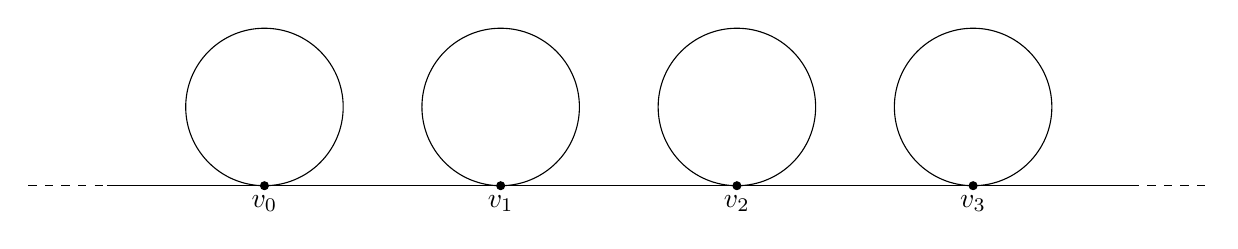
\begin{tikzpicture}
\draw (2,0) arc(0:360:1);
\draw (5,0) arc(0:360:1);
\draw (8,0) arc(0:360:1);
\draw (11,0) arc(0:360:1);
\draw[fill=black] (1.05,-1) arc(0:360:0.05);
\draw[fill=black] (4.05,-1) arc(0:360:0.05);
\draw[fill=black] (7.05,-1) arc(0:360:0.05);
\draw[fill=black] (10.05,-1) arc(0:360:0.05);
\draw (1,-1) node[below] {$v_0$};
\draw (4,-1) node[below] {$v_1$};
\draw (7,-1) node[below] {$v_2$};
\draw (10,-1) node[below] {$v_3$};
\draw (-1,-1) -- (12,-1);
\draw[dashed] (-2,-1) -- (-1,-1);
\draw[dashed] (12,-1) -- (13,-1);
\end{tikzpicture}
$$
and the identifications $v_i \sim v_{i+1}$ (note that these circles are supposed to be $2$-spheres). Then by a similar arhument as in (vi) $Y$ is simply connected, thus the universal covering.

\item The Klein bottle $K$ is covered by the $2$-Torus. Thus the universal covering of $K$ is $\mathbb{R}^2$.
\item The projective space $\mathbb{P}^2(\mathbb{R})$ is the quotient of the sphere $\mathbb{S}^2$ under the identification $x \sim -x$. Then $\mathbb{S}^2$ is the universal covering of $\mathbb{P}	^2(\mathbb{R})$.

\end{compactenum}
Now the coverings in (i)-(v) and in (viii) are contractible, i.e. homotopy equivalent. Those in (vi) and (ix) are not contractible. The space $Y$ in (vii) is neither contractible nor homotopy equivalent to the $2$-sphere. $\hfill \Box$
\end{sol}



\end{prob}    %%AUFGABE 1.2


\begin{prob} Compute the fundamental group $\pi_1(X,x_0)$ when $X$ is the space from (i), (ii), (iii), (iv), (vi), (vii) or (ix) in the first problem. \textit{Hint: For (vi) and (vii) you may use that every continuous map $\mathbb{S}^1 \la \mathbb{S}^2$ is homotopic to a nonsurjective one}.

\begin{sol}
\begin{compactenum}
\item Recall from EGT that for the universal covering $p: Y \la X$ we have
$$\mathrm{Deck}(p) := \left\{ \phi: Y \la Y \ \vert \ \phi \textrm{ is a homeomorphism with }p\circ \phi = p \right\} \cong \pi_1(X,x_0)$$
and $\pi_1(X,x_0) = \pi_1(X,\tilde{x}_0)$ for $x_0, \tilde{x}_0$ contained in the same path component. We now claim that 
$$\mathrm{Deck}(p) \overset{!}{=} \left\{ \phi_n: \mathbb{R} \la \mathbb{R}, \ x \mapsto x+n \ \vert \ n \in \Z \right\} \cong \Z.$$
Clearly $\phi_n \in \mathrm{Deck}(p)$ since these are homeomorphisms satisfying $p \circ \phi = p $. Let conversely $\phi \in \mathrm{Deck}(p)$. Then 
$$1=p(0)= (p \circ \phi)(0) = e{2 \pi i \phi(0)}$$
and we may define $n:= \phi(0) \in \Z$. Thus $\phi$ and $\phi_n$ agree at $x=0$. But this implies $\phi=\phi_n$, since lift agreeing at one point are identical. Thus we computed
$$\pi_1(\mathbb{S}^1, x_0) =: \pi_1(\mathbb{S}^1) \cong \Z$$
for any $x_0 \in \mathbb{S}^1$.
\item We claim that $\mathbb{S}^1 \times [0,1]$ is homotopy equivalent to $\mathbb{S}^1$. Indeed define
$$h: X \times [0,1] = \mathbb{S}^1 \times [0,1]^2 \la \mathbb{S}^1 \times [0,1]= X, \qquad ((x,y),t) \mapsto (x, (1-t)y)$$
and 
$$\iota: \mathbb{S}^1 \la \mathbb{S}^1 \times [0,1], \qquad x \mapsto (x,0),$$
$$r: \mathbb{S}^1 \times [0,1] \la \mathbb{S}^1, \qquad (x,y) \mapsto x.$$
Then $r \circ \iota = \id_{\Sph^{1}}$ and 
$$h_0(x,y)=(x,y)=\id_{\Sph^1 \times [0,1]}(x,y), \qquad h_1(x,y) = (x,0) =(\iota \circ r)(x,y),$$
i.e. $\iota \circ r$ is homotopic to the identity map on $\mathbb{S}^1 \times [0,1]$. Hence $h$ is a homotopy equivalence. Then we can conclude
$$\pi_1(\mathbb{S}^1 \times[0,1],x_0) =: \pi_1(\mathbb{S}^1 \times [0,1]) \cong \pi_1(\mathbb{S}^1) \cong \Z.$$
\item The Möbius strip is also homotopy equivalent to the circle:
$$
\begin{tikzpicture}
\draw (-6,0) -- (-4,0);
\draw[->] (-4,0) -- (-4,1);
\draw (-4,1) -- (-4,2);
\draw (-4,2) -- (-6,2);
\draw[->] (-6,2) -- (-6,1);
\draw (-6,1) -- (-6,0);

\draw[->] (-3,1) -- (-1,1);

\draw (0,0) -- (2,0);
\draw[->] (2,0) -- (2,1);
\draw (2,1) -- (2,2);
\draw (2,2) -- (0,2);
\draw[->] (0,2) -- (0,1);
\draw (0,1) -- (0,0);
\draw[thick] (0,1) -- (2,1);
\draw[->] (0.5,0.25) -- (0.5,0.75);
\draw[->] (1,0.25) -- (1,0.75);
\draw[->] (1.5,0.25) -- (1.5,0.75);
\draw[->] (0.5,1.75) -- (0.5,1.25);
\draw[->] (1,1.75) -- (1,1.25);
\draw[->] (1.5,1.75) -- (1.5,1.25);
\end{tikzpicture}
$$
The idea is to retract the square to the middle, which under identification of the endpoints defines a circle. More precisely let 
$$h: M \times [0,1] \la M, \qquad ((x,y),t) \mapsto (1-t)(x,y) + t \left( x, \frac{1}{2}\right)$$
and
$$\iota: \mathbb{S}^1 \cong \mathbb{S}^1 \times \left\{ \frac{1}{2}\right\} \hookrightarrow M, \qquad \left( x, \frac{1}{2}\right) \mapsto \left( x, \frac{1}{2}\right),$$
$$r: M  \la \mathbb{S}^1 \times \left\{ \frac{1}{2}\right\}, \qquad (x,y) \mapsto \left( x, \frac{1}{2}\right).$$
Then $r \circ \iota = \id_{\Sph^1}$ and 
$$h_0(x,y) = (x,y) = \id_{M}(x,y), \qquad h_1(x,y) = \left(x, \frac{1}{2}\right),$$
i.e. $\iota \circ r$ is homotopic to the identity map on $M$. Hence $h$ is a homotopy equivalence and we conclude
$$\pi_1(M,x_0) =: \pi_1(M) \cong \pi_1(\mathbb{S}^1) \cong \Z.$$
\item For the $2$-Torus we easily verify
$$\pi_1(\mathbb{T}^2, x_0) = \pi_1(\mathbb{T}^2) = \pi_1(\mathbb{S}^1 \times \mathbb{S}^1) = \pi_1(\mathbb{S}^1) \times \pi_1(\mathbb{S}^1) \cong \Z^2.$$
\item[(vi)] We saw in problem 1 that $\pi_1(\mathbb{S}^2,x_0) \cong \{0\}$. 
\item[(vii)] We claim that $\pi_1(\mathbb{S}^1 \vee \mathbb{S}^2,x_0) \cong \Z.$ By using the hint any loop $[\alpha]$ in $\mathbb{S}^1 \vee \mathbb{S}^2$ misses a point on the $2$-sphere. By the same arguments as seen before, $\alpha$ is homotopic to a loop with image completely in the circle, i.e. 
$$\pi_1(\mathbb{S}^1 \vee \mathbb{S}^2, x_0) \cong \pi_1(\mathbb{S}^1 \vee \mathbb{S}^2) \cong \pi_1(\mathbb{S}^1) \cong \Z.$$
\item[(ix)] We claim that $\pi_1(\mathbb{P}^2(\mathbb{R}),x_0) \cong \slant{\Z}{2 \Z}$ for all $x_0 \in \mathbb{P}^2(\mathbb{R})$. as in (i) we use that 
$$\pi_1(\mathbb{P}^2(\mathbb{R},x_0) = \pi_1(\mathbb{P}^2(\mathbb{R}) \cong \mathrm{Deck}(p) \cong \left\{ \phi: \mathbb{S}^2 \la \mathbb{S}^2 \ \vert \ p \circ \phi = p\right\} \overset{!}{\cong} \{ \id_{\Sph^2}, -\id_{\Sph^2} \} = \slant{\Z}{2\Z}.$$
Clearly the identity and the antipodal map are deck transformations. To see other inclusion let $\phi \in \mathrm{Deck}(p)$. Then using the fact that $p$ is the quotient map we have 
$$\pm x = [p] = p(x)=(p \circ \phi)(x) = [\phi(x)] = \pm \phi(x),$$
i.e. $\phi(x) = \pm x$ which was to be shown. $\hfill \Box$
\end{compactenum}
\end{sol}


\end{prob}


\begin{prob}   %%AUFGABE 1.3
Let $p: Y \la X$ be a covering space.
\begin{compactenum}
\item Show that $p$ is an open map, i.e. images of open sets in $Y$ under $p$ are open in $X$.
\item Assume that $X$ is locally connected, i.e. for every point $x \in X$ and every open set $U \subseteq X$ containing $x$ there exists an open, connected set $V \subseteq U$ containing $x$. Show that in this case $Y$ is locally connected as well.
\item Let $A \subseteq X$ be a subspace and $B= p^{-1}(A)$. Show that $p\vert_B: B \la A$ is a covering space.
\end{compactenum}
\begin{sol}
\begin{compactenum}
\item Let $V \subseteq Y$ be open and $x \in p(V)$, say $x= p(y)$. Chosse a covering neighbourhood $U \subseteq X$ of $x$ with preimage 
$$p^{-1}(U) = \bigcup^{\cdot}_{i \in I} V_i$$
and homeomorphisms $p\vert_{V_i}: V_i \la U$ for all $i \in I$. Chose $i_0 \in I$ with $y \in V_{i_0}$. Since $p(V_{i_0} \cap V)$ is open in $U$ and thus, since $U$ is open, in $X$, $V \cup V_{i_0}$ is open in $Y$. Thus $x \in p(V_{i_0}\cap V)$ is an interior point of $p(V)$ which implies the claim.
\item Let $y \in Y$ be any point and $V \subseteq Y$ an open subseteq of $Y$ containing $y$. We have to find an open, connected set $\tilde{V} \subseteq Y$ containing $y$ and contained in $V$. Choose a covering neighbourhood $U\subseteq X$ of $p(y)$ with preimage 
$$p^{-1}(U) = \bigcup^{\cdot}_{i \in I} V_i$$
and $y \in V_{i_0}$. Since $p\vert_{V_{i_0}} \la U$ is a homeomorphism, $p(V \cap V_{i_0}) \subseteq U$ is open in $U$, thus open in $X$. Since $X$ is locally connected, we an find an open neighbourhood $W\subseteq X$ of $p(y)$ with $W \subseteq p\vert_{V_{i_0}}(V \cap V_{i_0})$. But then $p\vert_{V_{i_0}}^{-1}(W) =: \tilde{V}$ is open and connnected in $Y$ with $y \in \tilde{V}$ and $\tilde{V} \subseteq V$, i.e. $Y$ is locally connected.
\item Clearly $\p\vert_{B}: B \la A$ is continuous and surjective, hence we only have to show the preimage property. Let $x \in A \subseteq X$. Since $p$ is a covering, we can choose a covering neighbourhood $U \subseteq X$ of $X$  such that 
$$p^{-1}(U) = \bigcup_{i \in I}^{\cdot} B_i.$$
But then $U \cap A$ is open in $A$ and 
$$p\vert_B ^{-1}(U \cap A) = p^{-1}(U \cap A) = p^{-1}(U) \cap p^{-1}(A) = \left( \bigcup_{i\in I}^{\cdot} B_i\right) \cap p^{-1}(A) = \bigcup_{i \in I}^{\cdot} V_i \cap p^{-1}(A)$$
is an open and disjoint union of open sets which project homeomorphically onto $U \cap A$ under $p\vert_{B}$. $\hfill \Box$

\end{compactenum}
\end{sol}



\end{prob}


\begin{prob}    %%AUFGABE 1.4
Find three different connected two-sheeted coverings of the $2$-torus $\mathbb{T}^2$, Does $\mathbb{T}^2$ have more four-sheeted of more five-sheeted connected coverings?
\begin{sol}
Recall: Let $X$ be a path connected, locally path connected and semi locally simply connected topological space. Then connected coverings of $X$ (more precisely: isomorphism classes of coverings of $X$) are inbijection with subgroups of $\pi_1(X)$. Thus index-$k$-subgroups of the fundamental group correspond to $k$-sheeted coverings.\\
Now the $2$ torus satisfies the assumptions above, i.e. we now have to find index-$2$-subgroups of $\pi_1(\mathbb{T}^2) \cong \Z^2$. Consider
\begin{compactenum}
\item $U_1 = 2\Z \times \Z \subseteq \Z^2$,
\item $U_2 = \Z \times 2\Z \subseteq \Z^2$,
\item $U_3 = \{(m,n) \in \Z^2 \ \vert \ m+n \in 2\Z\}$.
\end{compactenum}
Instantly, for the first case we can write down the covering; it is given by
$$p_1: \Sph^1 \times \Sph^1 \la \Sph^1 \times \Sph^1, \qquad (z_0, z_1) \mapsto (z_0^2, z_1).$$
Then the induced map on the fundamental groups is 
$$p_1* = \pi_1(p): \pi_1(\mathbb{T}^2) \la \pi_1(\mathbb{T}^2)$$
and has image $p_1*(\pi_1(\mathbb{T}^2) \cong 2\Z \times \Z$. We can do it analogously for the other coverings. To give an answer to the last question, w have to find out whether there are more index-$4$- or index-$5$-subgroups of $\Z^2$. Algebraic methods give us there are $7$ rsp. $6$ subgroups, i.e. there are more $4$-sheeted coverings than $5$-sheeted ones. $\hfill \Box$
\end{sol}

\end{prob}





\newpage


\titlespacing*{\section}{-16.5pt}{0pt}{20pt}
\renewcommand*\thesection{}
\section{Problem set 2} %PARAGRAPH A.2
\renewcommand*\thesection{\arabic{section}}



\begin{prob}     %%ASUFGABE 2.1
Let $G$ be the group given by the presentation 
$$G= \langle a,b,c \ \vert \ a^3,b^3,c^4,acac^{-1},aba^{-1}bc^{-1}b^{-1} \rangle.$$
Show that $G$ is the trivial group \textit{(Hint: Expand $(aba^{-1})^3 = (bcb^{-1})^3$)}.
\begin{sol}
We calculate
$$e=aa^{-1} = ab^3a^{-1}=(aba^{-1})^3=(bcb^{-1})^3 = bc^3b^{-1} = bc^{-1}b^{-1},$$
thus $c^{-1}=e$, i.e. $c=e$. Then 
$$e=acac^{-1}=a^2 = a^{-1}$$
and the same holds for $a$. Finally
$$e=aba^{-1}bc^{-1}b^{-1} = b^2c^{-1}b^{-1} = b$$
and all the generators must be the neutral element, thus $G=\{e\}$. $\hfill \Box$
\end{sol}
\end{prob}



\begin{prob}  %% AUFGABE 2.2
Let $G$ be the group given by the presentation 
$$G= \langle a,b \ \vert \ b^{-1}a^3b = a^5 \rangle$$
Let $\phi: G \la H$ be a homomorphism of groups into a finite group $H$ and let $g \in G$ be given by the word $g=a^{-1}b^{-1}a^{-1}bab^{-1}ab$. Show that $g \in \ker \phi$. \textit{(Hint: Write $s=\phi(a)$.We have $s^n=1$ for some $n$ and we can assume $\mathrm{gcd}(n,3)=1$. Why? What does it help?)}
\begin{sol}
Write $s=\phi(a)$. Since $H$ is finite, there exists a smallest $n \in \mathbb{N}_0$ such that $s^n = e_H$. Assume that $\mathrm{gcd}(n,3) \neq 1$. Then $\mathrm{gcd}(n,3)=3$ and thus $3 \vert n$, i.e. we can write $n=3m$ for some $m \in \mathbb{N}_0$. Then 
$$e_H= s^n = s^{3m} = \phi(a)^{3m} = \phi(a^{3m}) = \phi(ba^{5m}b^{-1}) = \phi(b) s^{5m} \phi(b)^{-1},$$
i.e. $s^{5m} = \phi(b)^{-1} \phi(b) = e_H$. But then
$$e_H = e_H e_H = s^{-3m} s^{5m} = s^{2m},$$
which contradicts minimality of $n$. Now that $n$ and $3$ are coprime, $s^3$ generates the cyclic group generated by $s$, i.e. $\langle s^3 \rangle = \langle s \rangle = \{e_H, s, s^{2}, \ldots, s^{n-1} \}$. In particular, we find $k \in \mathbb{N}_0$ satisfying $s=(s^3)^k = s^{3k}$. Then
$$\phi(b^{-1}ab) = \phi(b)^{-1} s \phi(b) = \phi(b)^{-1} s^{3k} \phi(b) = \left( \phi(b)^{-1} s^3 \phi(b)\right)^k =\phi(b^{-1}a^3b)^k = \phi(a)^{5k} = s^{5k}$$
and thus
\begin{alignat*}{5}
\phi(g) \ \ &=&& \ \ \phi(a^{-1}b^{-1}a^{-1}bab^{-1}ab) \\
&=&& \ \ \phi(a^{-1} (b^{-1}a^{-1}b) a (b^{-1}ab))\\
&=&& \ \ \phi(a)^{-1} \phi(b^{-1}a^{-1}b) \phi(a) \phi(b^{-1}ab) \\
&=&& \ \ s^{-1} \phi(b^{-1}ab)^{-1} s \phi(b^{-1}ab) \\
&=&& \ \ s^{-1}s^{-5} s s^{5} \\
&=&& \ \ e_H,
\end{alignat*}
which proves the claim. $\hfill \Box$
\end{sol}


\end{prob}



\begin{prob}   %%AUFGABE 2.3
Leg $G$ be a group and denote by $\underline{G\textrm{-}\mathrm{sets}}$ the category of left $G$-sets (recall that objects are functors from $\underline{G}$ to $\sets$ and morphisms are natural transformations).
\begin{compactenum}
\item What interesting functors are there (in either direction) between $\sets$ and $\underline{G\textrm{-}\mathrm{sets}}$? Which of those functors are adjoint to which?
\item Similarly, what interestig functors are there between $\kvec$ and the category $\underline{G\textrm{-}k\textrm{-}\mathrm{vec}}$ of $k$-linear representations of $G$ and what adjunctions are there between those functors?
\end{compactenum}
\begin{sol}
We will profoundly discuss the first part of the problem. The second one works similarly.
\begin{compactenum}
\item We have functors
$$\mathcal{U}: \gsets \la \sets, \qquad \begin{cases} \ (\F: \underline{G} \la \sets) \mapsto \mathcal{U}(\F)=\F(\cdot), \\ \ (\alpha: \F \la \G) \mapsto (\mathcal{U}(\alpha)= \alpha_{\cdot}: \F(\cdot) \la \G(\cdot)) \end{cases}$$
and $\mathcal{V}: \sets \la \gsets$ defined on objects by
$$ S \mapsto \left( \mathcal{V}(S): \underline{G} \la \gsets, \ \ \begin{cases} \ \cdot \mapsto G \times S, \\ \ g \mapsto \left(\mathcal{V}(S)(g): G \times S \la G \times S, \ (h,s) \mapsto (gh,s)\right) \end{cases}\right)$$
and on morphisms by 
$$(f: S \la T) \mapsto \left( \mathcal{V}(f) = \begin{cases} \ \alpha: \mathcal{V}(S) \la \mathcal{V}(T), \\ \ \alpha_.: \mathcal{V}(S)(\cdot) = G \times S \la G \times T, \ \ (g,s) \mapsto (g,f(s)) \end{cases} \right)$$
We now claim that $\mathcal{V}$ is a left adjoint to $\mathcal{U}$. Therefore define

$$\Phi: \Hom_{\gsets}(\mathcal{V}(S),\mathcal{F}) \la \Hom_{\sets}(S, \mathcal{U}(\mathcal{F}))$$
by 
$$\begin{rcases} \alpha: \mathcal{V}(S) \la \F, \\ \alpha_.: \G \times S \la \F(\cdot) \end{rcases} \ \ \mapsto \Phi(\alpha)= \begin{cases} \ S \la \mathcal{U}(\F) = \F(\cdot), \\ \ s \mapsto \alpha_.(1,s) \end{cases}$$
and 
$$\tilde{\Phi}: \Hom_{\sets}(S, \mathcal{U}(\F)) \la \Hom_{\gsets}(\mathcal{V}(S), \F)$$
by
$$(f: S \la \F(\cdot) ) \mapsto \tilde{\Phi} = \begin{cases} \ \alpha: \mathcal{V}(S) \la \F, \\ \ \alpha_.: G \times S \la \F(\cdot), \ (g,s) \mapsto \F(g)(f(s)) \end{cases}$$
We have to show that $\Phi$ and $\tilde{\Phi}$ are inverse to each other. On the one hand, for a natural transformation $\alpha$ we have 
$$\left( \tilde{\Phi} \circ \Phi\right)(\alpha) = \begin{cases} \ (\tilde{\Phi} \circ \Phi)(\alpha) : \mathcal{V}(S) \la \F, \\ \ (\tilde{\Phi} \circ \Phi)(\alpha)_.: G \times S \la \F(\cdot), \ (g,s) \mapsto \F(g) \alpha_.(1,s), \end{cases}$$
i.e. we have to show $\alpha_.(g,s) = \F(g)(\alpha_.(1,s))$ for all $g \in G$ and $s \in S$. But since $\alpha$ is a natural transformation, the diagram
$$
\begin{xy}
\xymatrix{
G \times S \ar[d]_{\alpha_.} \ar[rr]^{\mathcal{V}(S)(g)}_{(h,s) \mapsto (gh,s)} && G \times S \ar[d]^{\alpha_.} \\ \F(\cdot) \ar[rr]_{\F(g)} && \F(\cdot)
}
\end{xy}
$$
commutes, i.e.
$$\alpha_.(g,s) = \alpha_.(\mathcal{V}(S)(g))(1,s) = \F(g)(\alpha_.(1,s)),$$
which proves $\tilde{\Phi} \circ \Phi = \id_{\Hom_{\gsets}(\mathcal{V}(S), \F)}$. Conversely for a map $f:S\la \F(\cdot)$ we have
$$(\Phi \circ \tilde{\Phi})(f) = \begin{cases} \ (\Phi \circ \tilde{\Phi})(f): S \la \F(\cdot), \\
\ s \mapsto \F(1)(f(s)) \end{cases} $$
But since $\F$ is a funcotr, $\F(1)= \id_{\F(\cdot)}$ and this gives $(\Phi \circ \tilde{\Phi})(f) = f$. All in all we proved that $\mathcal{V}$ is a left adjoint to $\mathcal{U}$. 


\item Consder for example the functor $\mathcal{U}: \gkvec \la \kvec$ with 
$$(\F: \underline{G} \la \kvec) \mapsto \mathcal{U}(\F) = \F(\cdot)$$
on objects and 
$$(\alpha: \F \la \G) \mapsto \left( \alpha_.: \F(\cdot) \la \G(\cdot)\right)$$
on morphisms. Let further $\mathcal{V}: \kvec \la \gkvec$ be the functor with 
$$V \mapsto \mathcal{V}(V) = \F: \underline{G} \la \kvec, \ \begin{cases} \ \cdot \mapsto V, \\ \ g \mapsto \id_V \end{cases}$$
on objects and 
$$(f:V \la W) \mapsto \mathcal{V}(f) = \begin{cases} \ \alpha: \mathcal{V}(V) \mapsto \mathcal{V}(W), \\ \ \alpha_. = f: V \la W \end{cases} $$
on morphisms. Then one verifies that $\mathcal{V}$ is a left adjoint to $\mathcal{U}$. $\hfill \Box$



\end{compactenum}

\end{sol}




\end{prob}


\begin{prob}     %%AUFGABE 2.4
A \textit{permutation} of a set $X$ is a bijection $X \la X$. Write $\mathcal{S}ym(X)$ for the set of permutations of $X$. A \textit{total order} on a set $X$ is an order "$\leqslant$" such that for all $x,y \in X$ either $x \leqslant y$ or $y \leqslant x$; so a total order on a finite set amounts to a way of placing its element in sequence. Write $\mathcal{O}rd(X)$ for the set of total orders on $X$. Let further $\underline{\mathrm{Fin}\textrm{-}\mathrm{Bij}}$ denote the category of finite sets and bijections.
\begin{compactenum}
\item Give a definition of $\mathcal{S}ym$ on maps in $\finbij$ in such a way that $\mathcal{S}ym$ becomes a functor $\finbij \la \sets$. Do the same for $\mathcal{O}rd$. Both your definitions should be canonical.
\item Show that there is no natural transformation $\mathcal{S}ym \la \mathcal{O}rd$ \textit{(Hint: Consider identity permutations)}.
\item For an $n$-element set $X$, how many elements do the sets $\mathcal{S}ym(X)$ and $\mathcal{O}rd(X)$ have?
\item Conclude that $\mathcal{S}ym(X) \cong \mathcal{O}rd(X)$ for all $X \in \finbij$, but not \textit{naturally}. The moral is that for each finite set $X$ there are exactly as many permutations of $X$ as there are total orders on $X$, but there is natural way of matching them up.
\end{compactenum}

\begin{sol}
\begin{compactenum}
\item Define $\mathcal{S}ym: \finbij \la \sets$ on morphisms by
$$(f: X \la Y) \mapsto (\mathcal{S}ym(f): \mathcal{S}ym(X) \la \mathcal{S}ym(Y), \quad g \mapsto f \circ g \circ f^{-1})$$
and $\mathcal{O}rd: \finbij \la \sets$ on morphisms by 
$$(f: X \la Y) \mapsto (\mathcal{O}rd(f): \mathcal{O}rd(X) \la \mathcal{O}rd(Y), \quad (x_{i_1}, \ldots, x_{i_n}) \mapsto \left(f(x_{i_1}), \ldots, f(x_{i_n})\right) $$
These assignments are clearly functorial. 

\item Assume there exists a natural transformation $\alpha: \mathcal{S}ym \la \mathcal{O}rd$. Consider $X=\{1,2\} \in \mathrm{ob}(\finbij)$ and $(f: X \la X, \ 1 \mapsto 2, \ 2 \mapsto 1) \in \Hom_{\finbij}(X,X)$. Then the diagram
$$
\begin{xy}
\xymatrix{
\mathcal{S}ym(\{1,2\}) \ar[rr]^{\mathcal{S}ym(f)} \ar[d]_{\alpha_{\{1,2\}}} && \mathcal{S}ym(\{1,2\}) \ar[d]^{\alpha_{\{1,2\}}} \\ \mathcal{O}rd(\{1,2\}) \ar[rr]_{\mathcal{O}rd(f)} && \mathcal{O}rd(\{1,2\})
}
\end{xy}
$$
must commute. Then 
$$\left( \alpha_{\{1,2\}} \circ \mathcal{S}ym(f)\right)\left(\id_{\{1,2\}}\right) = \alpha_{\{1,2\}}\left( f \circ \id_{\{1,2\}} \circ f^{-1}\right) = \alpha_{\{1,2\}}\left(\id_{\{1,2\}}\right)$$
and 
$$\left( \mathcal{O}rd(f) \circ \alpha_{\{1,2\}} \right) \left(\id_{\{1,2\}}\right) = \mathcal{O}rd(f) \left( \alpha_{\{1,2\}}\left(\id_{\{1,2\}}\right)\right).$$
This implies 
$$(2,1) = (f(1), f(2)) = \mathcal{O}rd(f)\left((1,2)\right) \overset{!}{=} (1,2),$$
which is a contradiction.
\item It is well known that $\vert \mathcal{O}rd(X)\vert = n! = \vert \mathcal{S}ym(X)\vert$.
\item There is no natural transformation, in particular no natural isomorphisms between the functors $\mathcal{S}ym$ and $\mathcal{O}rd$, i.e. they are not naturally isomorphic. However, $\mathcal{S}ym(X) \cong \mathcal{O}rd(X)$ by part (iii). $\hfill \Box$
\end{compactenum}

\end{sol}

\end{prob}











\newpage




\titlespacing*{\section}{-16.5pt}{0pt}{20pt}
\renewcommand*\thesection{}
\section{Problem set 3} %PARAGRAPH A.3
\renewcommand*\thesection{\arabic{section}}



\begin{prob}     %%ASUFGABE 3.1
Let $\C$ and $\D$ be categories and let $\G: \D \la \C$ be a functor with left adjoint $\F: \C \la \D$. Let $D: \mathcal{I} \la \D$ be a diagram of shape $\mathcal{I}$ and suppose it has the limit $\left(\lim D, (p_i: \lim D \la D(i))_{i \in \mathrm{ob}(\mathcal{I})}\right)$. In this exercise e will show step by step that the diagram $\G \circ D$ has limit 
$$ \lim \G \circ D = \left( \G(\lim D), (\G(p_i): \G(\lim D) \la \G(D(i)))_{i \in \mathrm{ob}(\mathcal{I})} \right).$$
\begin{compactenum}
\item Show that the above defines a cone of $\G \circ D$. 
\item Let $\left(C, (f_i: C \la \G(D_i))_{i \in \mathrm{ob}(\I)}\right)$ be any other cone. Show that naturality of the adjunction implies that the adjunct morphisms form a cone on $D$.
\item Conclude that there is a unique morphism $\F(C) \la \lim D$ factorizing the cone $\F(C)$ over the universal cone $\lim D$ and show that its adjunct gives the desired unique arrow factorizing the cone $C$ over the cone $\G(\lim D)$. 

\end{compactenum}

\begin{sol}
Let 
$$\Phi_{CG}: \Hom_{\C}(C,\G(G)) \overset{\cong}{\la} \Hom_{\D}(\F(C),G), \qquad f \mapsto \overline{f}$$
be the adjunction.
\begin{compactenum}
\item We need to show that the diagram
$$
\begin{xy}
\xymatrix{
& \G(\lim D) \ar[rd]^{\G(p_j)} \ar[ld]_{\G(p_i)} & \\ \G(D(i)) \ar[rr]_{\G(D(g_{ij}))} && \G(D(j))
}
\end{xy}
$$
commutes for all $g_{ij} \in \Hom_{\I}(i,j)$. But this immidiately follows from functoriality of $\G$ and from the fact that $\lim D$ is a cone:
$$\G(D(g_{ij})) \circ \G(p_i) ) \G(D(g_{ij}) \circ p_i) = \G(p_j).$$


\item Let $\left(f_i: C \la \G(D_i)\right)_{i \in \mathrm{ob}(\I)}$ be a cone on $\G \circ D$. We have to show, that the adjoint morphisms $\left(\overline{f}_i: \F(C) \la D(i)\right)_{i \in \mathrm{ob}(\I)}$ form a cone on $D$, i.e. that the diagram
$$
\begin{xy}
\xymatrix{
& \F(C) \ar[rd]^{\overline{f}_j} \ar[ld]_{\overline{f_i}} & \\ D(i) \ar[rr]_{D(g_{ij})} && D(j) }
\end{xy}
$$
commutes for all $g_{ij} \in \Hom_{\I}(i,j)$. Consider 
$$
\begin{xy}
\xymatrix{
\Hom_{\C}(C, \G(D(i))) \ar[d]_{\G(D(g_{ij}))} \ar[rr]^{\Phi_{CD(i)}} && \Hom_{\D}(\F(C), D(i)) \ar[d]^{D(g_{ij})} \\ \Hom_{\C}(C, \G(D(j))) \ar[rr]_{\Phi_{CD(j)}} && \Hom_{\D}(\F(C), D(j))
}
\end{xy}
$$
Then 
$$\overline{f}_j = \overline{\G(D(g_{ij})) \circ f_i} = \left( \Phi_{CD(j)} \circ \G(D(g_{ij}))\right)(f_i) \overset{!}{=} \left( D(g_{ij}) \circ \Phi_{CD(i)}\right)(f_i) = D(g_{ij}) \circ \overline{f}_i,$$
which shows the desired property.

\item Now since $\left( (\F(C),(\overline{f}_i: \F(C) \la D(i))_{i \in \mathrm{ob}(\I)}\right)$ defines a cone on $D$, there exists a unique morphism $\overline{\phi}: \F(C) \la \lim D$ do make the following diagram commutative:
$$
\begin{xy}
\xymatrix{
& \F(C) \ar@/^{20pt}/[rdd]^{\overline{f_j}} \ar@/_{20pt}/[ldd]_{\overline{f}_i} \ar[d]^{\overline{\phi}} & \\ & \lim D \ar[rd]^{p_j} \ar[ld]_{p_i} & \\ D(i) \ar[rr]_{D(g_{ij})} && D(j) 
}
\end{xy}
$$
Now there is unique corresponding morphism $\phi: C \la \G( \lim D)$. We show, that this is the right arrow factorizing the cone $C$ over $\G(\lim D)$, i.e. that the diagram
$$
\begin{xy}
\xymatrix{
& C \ar[d]^{\phi} \ar@/^{20pt}/[rdd]^{f_j} \ar@/_{20pt}/[ldd]_{f_i} & \\ &  \G(\lim D) \ar[rd]^{\G(p_j)} \ar[ld]_{\G(p_i)} & \\ \G(D(i)) \ar[rr]_{\G(D(g_{ij}))} && \G(D(j))
}
\end{xy}
$$
becomes commutative. But again by naturality of the adjunction, the diagram
$$
\begin{xy}
\xymatrix{
\Hom_{\C}(C, \G(\lim D)) \ar[rr]^{\Phi_{C\lim D}} \ar[d]_{f \mapsto \G(p_i) \circ f} && \Hom_{\D}(\F(C), \lim D) \ar[d]^{f \mapsto p_i \circ f} \\ \Hom_{\C}(C, \G(D(i))) \ar[rr]_{\Phi_{CD(i)}} && \Hom_{\D}(\F(C), D(i))
}
\end{xy}
$$
commutes. Then for $\phi \in \Hom_{\C}(C, \G(\lim D))$ we have 
$$\G(p_i) \circ \phi = \left( \Phi_{CD(i)}^{-1} \circ (p_i \circ ) \circ \Phi_{C \lim D} \right) (\phi) = \Phi_{CD(i)}^{-1}(p_i \circ \overline{\phi}) = \Phi_{CD(i)}^{-1}(\overline{f}_i) = f_i,$$
i.e. the cone $\left(C, (f_i:C \la \G(D(i)))_{i \in \mathrm{ob}(\I)}\right)$ factorizes over $\G (\lim D)$. It remains to show that $\phi$ is unique. But this is clear: Suppose $\phi_1, \phi_2: C \la \G (\lim D)$ are two such morphisms. The the adjoint morphisms $\overline{\phi}_1, \overline{\phi}_2: \F(C) \la \lim D$ make the diagram
$$
\begin{xy}
\xymatrix{
& \F(C) \ar@/^{20pt}/[rdd]^{\overline{f_j}} \ar@/_{20pt}/[ldd]_{\overline{f}_i} \ar[d]^{\overline{\phi}_1} _{\overline{\phi}_2}& \\ & \lim D \ar[rd]^{p_j} \ar[ld]_{p_i} & \\ D(i) \ar[rr]_{D(g_{ij})} && D(j) 
}
\end{xy}
$$
commute. But then $\phi_1 = \phi_2$ and by bijectivity $\phi_1 = \phi_2$. 


\end{compactenum}


\textit{Remark: We thus have shown that a right adjoint functor $\G$ is continuous: It preserves all (small) universal cones and in particular we have}
$$\G (\lim D) = \lim (\G \circ D).$$
\textit{Dually, a left adjoint functor $\F$ is cocontinuous: It preserves all (small) universal cocones and in particular we have}
$$\F (\mathrm{colim} \ D) = \mathrm{colim} \ (\F \circ D).$$


\end{sol}

\end{prob}







\begin{prob}   %%AUFGABE 3.2
Let $\G: \topsp \la \sets$ be the forgetful functor. We claimed that the pullback in $\topsp$ corresponds to the pullback in $\sets$ under $G$. Prove this now by constructing a left adjoint functor to $\G$ (and using problem 3.9). Does $\G$ also have a right adjoint?
\begin{sol}
Define the functors
$$\F_1: \sets \la \topsp, \qquad \begin{cases} \ X \mapsto (X, \mathfrak{T}_{\mathrm{discrete}}), \\ \ (f: X \la Y) \mapsto f \end{cases} $$ 
and 
$$\F_2: \sets \la \topsp, \qquad \begin{cases} \ X \mapsto (X; \mathfrak{T}_{\mathrm{trivial}}), \\ \ (f: X \la Y) \mapsto f \end{cases} $$
Then we have adjunctions
$$\Hom_{\topsp}(\G(X), S) \overset{\cong}{\la} \Hom_{\sets}(X, \F_2(S))$$
and
$$\Hom_{\topsp}(S, \G(X)) \overset{\cong}{\la} \Hom_{\sets}(\F_1(S), X).$$
Thus $\F_ 2$ is a left adjoint to $\G$ and $\F_1$ is a right adjoint to $\G$. Then problem 3.9 gives us the claim. $\hfill \Box$

\end{sol}

\end{prob}




\begin{prob}    %%AUFGABE 3.3
Let $p_B: E \la B$ be a covering space and let $\phi: B' \la B$ be a continuous map. Show that the morphism $p_B': E_{\phi}: \la B'$ in the pullback square
$$
\begin{xy}
\xymatrix{
E_{\phi} \ar[d]_{p_B'} \ar[rr]^{\phi_E} && E \ar[d]^{p_B} \\ B' \ar[rr]_{\phi} && B
}
\end{xy}
$$
is again a covering space. \textit{(Hint: Recall the definition of $p_B: E \la B$ being a covering space: for each $x \in B$ we have an open neighbourhood $U \subseteq B$ of $x$, a discrete space $D$ and a homeomorphism $g: p_B^{-1}(U) \la D \times U$ which fits into the commutative triangle}
$$
\begin{xy}
\xymatrix{
p_B^{-1}(U) \ar[rr]^{g} \ar[rd]_{p_B} && D \times U \ar[ld]^{\mathrm{pr}_U} \\ & U &
} 
\end{xy}
$$
\textit{Out of this data construct correspondng triangles for $p_B': E_{\phi} \la B'$).}

\begin{sol}
Recall that 
$$E_{\phi} = \left\{ (e,b') \in E \times B' \ \vert \ \phi(b') = p_B(e) \right\}$$
and $p_B'$ is the projection $$p_B': E_{\phi} \la B', (e,b') \mapsto b'.$$
Let now $b' \in B'$ be arbitrary. Choose a neighbourhood $U \subseteq B$ of $\phi(b')$ and discrete space $D$ such that we obtain a commutative triangle
$$
\begin{xy}
\xymatrix{
p_B^{-1}(U) \ar[rr]^{g} \ar[rd]_{p_B} && D \times U \ar[ld]^{\mathrm{pr}_U} \\ & U & 
}
\end{xy}
$$
Now let $U':= \phi^{-1}(U) \subseteq B'$ and consider the triangle
$$
\begin{xy}
\xymatrix{
p_B'^{-1}(U') \ar[rr]^{h} \ar[rd]_{p_B'} && D \times U' \ar[ld]^{\mathrm{pr}_{U'}} \\ & U' & 
}
\end{xy}
$$
where
$p_B'^{-1}(U')  \subseteq E_{\phi}$ and $h$ is given by
$$h: p_B'^{-1}(U') \la D \times U', \qquad (e,b') \mapsto (\mathrm{pr}_D(g(e)), b')$$
and $p_B'$ is the projection onto the second component. Then the diagram obviously commutes. Morover $h$ is continuous with a continuous inverse 
$$\tilde{h}: D \times U' \la p_B'^{-1}(U'), \qquad (d,b') \mapsto \left( g^{-1}\left((d,\phi(b'))\right), b'\right).$$
Indeed for $(e,b') \in p_B'^{-1}(U')$ we have 
\begin{alignat*}{5}
(\tilde{h} \circ h)(e,b') \ \ &=&& \ \  \tilde{h}\left( \mathrm{pr}_D(g(e)), b'\right) \\
&=&& \ \ \left( g^{-1}\left((\mathrm{pr}_D(g(e)), \phi(b'))\right), b'\right) \\
&=&& \ \ \left( g^{-1}\left((\mathrm{pr}_D(g(e)), \mathrm{pr}_U(g(e)))\right), b'\right) \\
&=&& \ \ \left( g^{-1}(g(e)), b'\right)\\
&=&& \ \ (e,b')
\end{alignat*}
and for $(d,b') \in D \times U'$
\begin{alignat*}{5}
(h \circ \tilde{h})(d,b') \ \ &=&& \ \ h \left( g^{-1}(d, \phi(b')), b'\right) \\
&=&& \ \ \left( \mathrm{pr}_D\left(g\left( g^{-1}(d, \phi(b'))\right)\right), b'\right) \\
&=&& \ \ \left( \mathrm{pr}_D(d, \phi(b')), b'\right) \\ 
&=&& \ \ (d,b')
\end{alignat*}
i.e. $h$ is an homeomorphism. This finally shows that $p_B': E_{\phi} \la B'$ is a covering space. $\hfill \Box$
\end{sol}

\end{prob}





















\newpage

\titlespacing*{\section}{-16.5pt}{0pt}{20pt}
\renewcommand*\thesection{}
\section{Problem set 4} %PARAGRAPH B.4
\renewcommand*\thesection{\arabic{section}}





\begin{prob}      %%AUFGABE 4.1
Let $n \geqslant 3$. Show that the complement of finitely many points in $\mathbb{R}^n$ is simply connected.
\begin{sol}
Let $X=\{x_1, \ldots, x_m\}$. Choose $r>0$ such that $B_r(x_i) \cap B_r(x_j) = \emptyset$ for all $i,j \in \{1, \ldots, m\}$, $i\neq j$. Then $\mathbb{R}^n \setminus \{x_1, \ldots, x_m\}$ is homotopy equivalent to $\mathbb{R}^n \setminus \left( \bigcup_{i=1}^m B_r(x_i)\right)$. Then we obtain $\mathbb{R}^n$ by attaching balls to the space $\mathbb{R}^n \setminus \left( \bigcup_{i=1}^m B_r(x_i)\right)$. In other words we have pushout diagram
$$
\begin{xy}
\xymatrix{
\coprod_{i=1}^m \mathbb{S}^{n-1} \ar[dd]_{\iota} \ar[rr]^{\coprod_{i=1}^m f_i} && \mathbb{R}^n \setminus \left( \bigcup_{i=1}^m B_r(x_i)\right) \ar[dd] \\&& \\ \coprod_{i=1}^m \mathbb{D}^n \ar[rr] && \mathbb{R}^n
}
\end{xy}
$$
where for each $i \in \{1, \ldots, m\}$ we fix homeomorphisms $f_i: \mathbb{S}^{m-1} \la B_r(x_i)$. Then by van Kampen's theorem this yields to a pushout 

$$
\begin{xy}
\xymatrix{
\pi_1\left(\coprod_{i=1}^m \mathbb{S}^{n-1}\right) \ar[dd]_{\pi_1(\iota)} \ar[rr]^{\coprod_{i=1}^m \pi_1(f_i)} && \pi_1\left(\mathbb{R}^n \setminus \left( \bigcup_{i=1}^m B_r(x_i)\right)\right) \ar[dd] \\&& \\ \pi_1\left(\coprod_{i=1}^m \mathbb{D}^n\right) \ar[rr] && \pi_1\left(\mathbb{R}^n\right)
}
\end{xy}
$$
But $\mathbb{D}^n$ is contractible and $\mathbb{S}^{n-1}$ too, since $n \geqslant 3$. Thus we obtain 
$$0=\pi_1(\mathbb{R}^n) \cong \pi_1\left( \mathbb{R}^n \setminus \left( \bigcup_{i=1}^m B_r(x_i)\right) \right) \cong \pi_1(\mathbb{R}^n \setminus \{x_1, \ldots, x_m\}),$$
which proves the claim. $\hfill \Box$

\end{sol}
\end{prob}



\begin{prob}    %%AUFGABE 4.2
Let $X= \slant{\left( (\Sph^1 \times \Sph^1) \amalg (\Sph^1 \times \Sph^1) \right)}{\sim}$ where we identify an embedded circle $\Sph^1 \times \{x_0\}$ in one copy of $\Sph^1 \times \Sph^1$ with the same circle $\mathbb{S}^1 \times \{x_0\}$ in the other copy.
\begin{compactenum}
\item Find a presentation for $\pi_1(X,x_0)$ by applying van Kampen's theorem.
\item Instead of describing $X$ as a pushout of two spaces along a common subspace as above, one can alternatively describe $X$ as the product of two spaces. Find such a discription and use it to compute $\pi_1(X,x_0)$ again. Convince yourself that the two results define isomorphic groups.
\end{compactenum}

\begin{sol}
\begin{compactenum}
\item Consider the pushout
$$
\begin{xy}
\xymatrix{
\mathbb{S}^1 \times \{x_0\} \ar[rr] \ar[d]_{\iota} && \Sph^1 \times \Sph^1 \ar[d] \\ \Sph^1 \times \Sph^1 \ar[rr] && X 
}
\end{xy}
$$
Then the inclusion is a NDR, thus van Kampen's theorem gives us a corresponding pushout square
$$
\begin{xy}
\xymatrix{
\pi_1(\Sph^1 \times \{x_0\}) \ar[d] \ar[rr] && \pi_1(\Sph^1 \times \Sph^1) \ar[d] \\ \pi_1(\Sph^1 \times \Sph^1) \ar[rr] && \pi_1(X)
}
\end{xy}
$$
in $\grp$. Now $\Sph^1 \times \{x_0\}$ obviously is isomorphic to $\Sph^1$ and its fundamental group is isomorphic to $\Z= \langle a\ \vert \ \emptyset\rangle$. Further $\pi_1(\Sph^1 \times\Sph^1) = \pi_1(\Sph^1) \times \pi_1(\Sph^1) \cong \Z^2 =\langle a,b \ \vert \ aba^{-1}b^{-1}\rangle$. Then the diagram looks like
$$
\begin{xy}
\xymatrix{
\langle a \ \vert \ \emptyset \rangle \ar[rr]^{a \mapsto a_1}\ar[d]_{a \mapsto a_2} && \langle a_1, b_1 \ \vert \ a_1b_1a_1^{-1}b_1^{-1}\rangle \ar[d] \\ \langle a_2, b_2 \ \vert \ a_2b_2a_2^{-1}b_2^{-1} \rangle \ar[rr]&& \pi_1(X)
}
\end{xy}
$$
Then 
\begin{alignat*}{5}
\pi_1(X) \ \ &\cong&& \ \ \langle a_1, b_1, a_2, b_2 \ \vert \ a_1b_1a_1^{-1}b_1^{-1}, a_2b_2a_2^{-1}b_2^{-1}, a_1a_2^{-1} \rangle \\
&=&& \ \ \langle a_1, b_1, b_2 \ \vert \ a_1b_1a_1^{-1}b_1^{-1}, a_1b_2a_1^{-1}b_2^{-1} \rangle \\
&\cong&& \ \ \Z \times\left( \Z \star \Z\right).
\end{alignat*}
\item Alternatively think of two $2$-tori which put one on the other, identifying the upper most copies of $\Sph^1$. Then $X=\Sph^1 \times (\Sph^1 \vee \Sph^1)$ and we obtain 
$$\pi_1(X) =\pi_1(\Sph^1 \times (\Sph^1 \vee \Sph1)) \cong \pi_1(\Sph^1) \times \pi_1(\Sph^1 \vee \Sph^1) \cong \Z \times (\Z \star \Z),$$
which gives the same result as above. $\hfill \Box$

\end{compactenum}
\end{sol}

\end{prob}




\begin{prob}   %%AUFGABE 4.3
\begin{compactenum}
\item Let $K$ be the Klein bottle. Apply van Kampen's theorem to obtain a group presentation $G_1 = \langle a,b \ \vert \ R_1 \rangle $ of $\pi_1(K)$ by regarding $K$ as the space obtained from gluing a $2$-cell to $\Sph^1 \vee \Sph^1$.
\item Explain that the Klein bottle can also be obtained from gluing two Möbius strips along their boundaries.
\item Now obtain a second group presentation $G_2 = \langle c,d \ \vert \ R_2 \rangle $ of $\pi_1(K)$ via van Kamoen's theorem applied to the cover by the two (thickened) embedded Möbius strips which slightly overlap along their boundaries.
\end{compactenum}
\begin{sol}
Recall the comstruction of the Klein bottle by identification opposite sides of a square in the following way:
$$
\begin{tikzpicture}
\draw[postaction={decorate},decoration={
    markings,
    mark=at position .125 with {\arrow{latex}},
    mark=at position .375 with {\arrow{latex}},
    mark=at position .635 with {\arrowreversed{latex}},
    mark=at position .875 with {\arrow{latex}},
    }
  ]
    (0,0)  -- (2,0) node[midway, below] {$a$} --(2,2) node[midway, right] {$b$} --(0,2) node[midway, above] {$a$}  -- cycle node[midway, left] {$b$};

     



\end{tikzpicture}
$$

\begin{compactenum}
\item Attaching a $2$-cell to $\Sph^1 \vee \Sph^1$ means the pushout 
$$
\begin{xy}
\xymatrix{
\Sph^1 \ar[d] \ar[rr]^{f} && \Sph^1 \vee \Sph^1 \ar[d] \\ \mathbb{D}^2 \ar[rr]&& K
}
\end{xy}
$$
where $[f] \in \pi_1(\Sph^1 \vee \Sph^1)= \langle a,b \ \vert \ \emptyset\rangle$ is represented by $[aba^{-1}b]$. Then van Kampen's theorem for attachinf cells implies 
$$\pi_1(K) \cong \slant{\pi_1(\Sph^1 \vee \Sph^1)}{N([f])} \cong \langle a,b \ \vert \ aba^{-1}b \rangle.$$

\item Consider the cover $K=M_1 \cup M_2$

$$
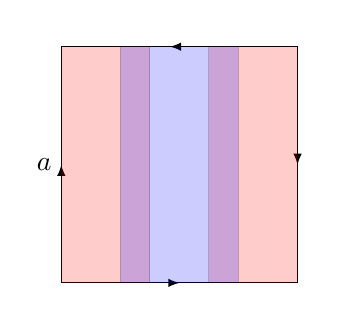
\begin{tikzpicture}[scale=1.5]
\draw[postaction={decorate},decoration={
    markings,
    mark=at position .125 with {\arrow{latex}},
    mark=at position .375 with {\arrowreversed{latex}},
    mark=at position .635 with {\arrow{latex}},
    mark=at position .875 with {\arrowreversed{latex}},
    }
  ]
    (0,0)  -- (2,0) node[midway, below] {$$} --(2,2) node[midway, right] {$$} --(0,2) node[midway, above] {$$}  -- cycle node[midway, left] {$a$};
    
\draw[fill=red,opacity=0.2] (0,0) -- (0.75,0) -- (0.75,2) -- (0,2) -- (0,0);
\draw[fill=red,opacity=0.2] (2,0) -- (2,2) -- (1.25,2) -- (1.25,0) -- (2,0);
\draw[fill=blue, opacity=0.2] (0.5,0) -- (1.5,0) -- (1.5,2) -- (0.5,2) -- (0.5,0);
\end{tikzpicture}
$$
where the red parts denote $M_1$ and the blue one denotes $M_2$.

\item Both $M_1$ and $M_2$ are homotopy equivalent to $\Sph^1$, as well as $M_1\cap M_2$ (note that $M_1 \cap M_2$ indeed is path connected!). However, going along $M_1 \cap M_2$ once means going $a$ (or $a^{-1}$) twice. Thus our pushout 
$$
\begin{xy}
\xymatrix{
M_1 \cap M_2 \ar[r] \ar[d] & M_1 \ar[d] \\M_2 \ar[r] & K
}
\end{xy}
$$
yields to 
$$
\begin{xy}
\xymatrix{
\langle a \ \vert \ \emptyset \rangle \ar[rr]^{a \mapsto b^2} \ar[d]_{a \mapsto c^2} && \langle b \ \vert \ \emptyset \rangle \ar[d] \\ \langle c \ \vert \ \emptyset \rangle \ar[rr] && \pi_1(K)
}
\end{xy}
$$
and we obtain 
$$\pi_1(K) \cong \langle b,c \ \vert \ c^2 b^{-2} \rangle,$$
a second presentation of $\pi_1(K)$. $\hfill \Box$
\end{compactenum}
\end{sol}

\end{prob}


\begin{prob} %%%AUFGABE 4.4
Of course the two group presentations resulting in Problem 4.14 deifne isomorphic groups. Give an exmplicit isomorphism and its inverse by writing down the images of $a$ and $b$ as ords in $c$ and $d$ and vice versa.
\begin{sol}
Define 
$$\phi: \langle a,b \ \vert \ \emptyset \rangle \la \langle c,d \ \vert \ cdc^{-1}d \rangle, \qquad a \mapsto c, \ \ b \mapsto d^{-1}c.$$
Then $\phi(a)=c$ and $\phi(ab^{-1}) =c (c^{-1}d) = d$, i.e. $\phi$ is surjective and 
$$\phi(a^2b^{-2}) = c^2 \left(d^{-1}c\right)^{-2} = c^2 (c^{-1}d)^2 = cdc^{-1}d = 0,$$
i.e. $\phi$ factorizes over $G_2$ and induces an surjective homomorphism
$$\overline{\phi}: \langle a,b \ \vert \ a^2b^{-2} \rangle \la \langle c,d \ \vert \ cdc^{-1}d \rangle.$$
Analogously we find that 
$$\psi \langle c,d \rangle \la \langle a,b \ \vert \ a^2b^{-2} \rangle, \qquad c \mapsto a, \ \ d \mapsto ab^{-1}$$
descends to a homomorphism 
$$\overline{psi}: \langle c,d \ \vert \ cdc^{-1}d \rangle \la \langle a,b \ \vert \ a^2b^{-2} \rangle.$$
Indeed, $\overline{\phi}$ and $\overline{\psi}$ are inverse to each other:
$$(\overline{\phi} \circ \overline{psi})(c) = \phi(a) = c, \qquad  (\overline{\phi} \circ \overline{psi})(d) = \overline{\phi}(ab^{-1}) = cc^{-1}d = d,$$
$$(\overline{\psi} \circ \overline{\phi})(a) \overline{\psi}(c) = a, \qquad (\overline{\psi} \circ \overline{\phi})(b) \overline{\psi}(ba^{-1}a) = b,$$
which shows the claim. $\hfill\Box$
\end{sol}
\end{prob}





















\newpage

\titlespacing*{\section}{-16.5pt}{0pt}{20pt}
\renewcommand*\thesection{}
\section{Problem set 5} %PARAGRAPH B.5
\renewcommand*\thesection{\arabic{section}}




\begin{prob} %%%AUFGABE 5.1
Proof the \textit{Lebesgue lemma}: Let $(X,d)$ be a compact, metric space with an open cover $\mathcal{U}=\{U_i \}_{i\in I}$. Then there exists a \textit{Lebesgue constant} $\delta >0$ such that every subset $A \subseteq X$ of diameter less than $\delta$ is contained in some $U_i \in \mathcal{U}$. \textit{(Hint: Start with a cover $X= \bigcup_{x \in X}B_{\epsilon(x)}(x)$ by open balls of radius $\epsilon(x)$ arround $x$ such that for each $x \in X$ the ball $B_{\epsilon(x)}(x)$ is contained in some $U_i \in \mathcal{U}$)}.
\begin{sol}
Since $X$ is compact, we can choose a finite subset of $\mathcal{U}$ as a cover, without loss of generality say $\{U_1, \ldots, U_\} \subseteq \mathcal{U}$. For each $i \in \{1, \ldots, n \}$ let $C_i:= X \setminus A_i$ and define a function 
$$f: X \la \mathbb{R}, \qquad x \mapsto f(x) := \frac{1}{n} \sum_{i=1}^n d(x,C_i).$$
Since $f$ is continuous and $X$ is compact, $f$ attains a minimum $\delta$ strictly greater than $0$. Now let $Y\subseteq X$ be a subset of diameter less than $\delta$. Then there exists $x_0 \in X$ such that $Y \subseteq B_{\delta}(x_0)$. The above implies $f(x_0) \geqslant \delta$, i.e. there exists $i \in \{1, \ldots, n \}$ such that $d(x_0, C_i) \geqslant \delta$. Butthis means $B_{\delta}(x_0) \cap C_i = \emptyset$, thus $$Y\subseteq B_{\delta}(x_0) \subseteq X \setminus C_i = A_i,$$
which proves the claim. $\hfill \Box$
\end{sol}
 
\end{prob}


\begin{prob}   %%AUFGABE 5.2
Let $C \subseteq \mathbb{R}^2$ be the union of circles $C_n$ of radius $\frac{1}{n}$ with center $\left( \frac{1}{n},0\right)$ for $n \in \mathbb{N}$ (the so call \textit{Hawaiian earring}). Show that $(C,(0,0))$ is now well pointed, i.e. the inclusion of the point $(0,0)$ into $C$ is not a neighbourhood defortmation retract. Is $C$ homeomorphic to $\bigvee_{n \in \mathbb{N}} \Sph^1$?
\begin{sol}
We have to show that no neighbourhood retracts onto $(0,0)$. Let $U \subseteq C$ be a neighbourhood of $(0,0)$. Then there exists $N \in \mathbb{N}$ such that $C_N \subseteq U$. Now define
$$r: U \la C_N, \qquad x \mapsto \begin{cases} \ x, & \textrm{ if } x \in C_N \\ \ (0,0), & \textrm{ otherwise. } \end{cases}$$
Then $r$ is continuous and a retraction onto $C_N$, i.e. we have $r \circ i_{C_N} = \id_{C_N}$. Then by functoriality of $\pi_1$ we have
$$\pi_1(r) \circ \pi_1(i_{C_N}) = \pi_1( r \circ i_{C_N}) = \pi_1(\id_{C_N}) = \id_{\pi_1(C_N)},$$
thus 
$$\pi_1(r): \pi_1(U) \la \pi_1(C_N) \cong \pi_1(\Sph^1) \cong \Z$$
is surjective (Recall that surjectivity of a composition requires the first map to be surjective). But then $\pi_1(U)$ cannot be trivial, thus $U$ cannot deformation retract onto $(0,0)$. \\

We now claim that $C$ is not homeomorphic to $\bigvee_{n \in \mathbb{N}} \Sph^1$. We first show that the latter is not compact. We exhibit a sequence which does not have any convergent subsequence. First fix homeomorphisms
$$f_n: \slant{[0,1]}{\partial [0,1]} \overset{\cong}{\la} \Sph^1, \qquad t \mapsto e^{2\pi i t}.$$
Then $\left\{x_n = f_n\left(\frac{1}{2}\right) \right\}_{n \in \mathbb{N}}$ is a sequence in $\bigvee_{n \in \mathbb{N}} \Sph^1$ which does not have any convergent subsequence. Now consider $C$ as the quotient of a compact space via the homeomorphism
$$f: \slant{[0,1]}{\left\{0,1,\frac{1}{2},\frac{1}{3}, \frac{1}{4}, \ldots, \right\}} \la C, \qquad$$
where $f \vert_{\left[\frac{1}{n+1}, \frac{1}{n}\right]}$ is defined as follows:
$$
\begin{xy}
\xymatrix{
\slant{\left[\frac{1}{n+1}, \frac{1}{n}\right]}{\frac{1}{n} \sim \frac{1}{n+1}} \ar[rr]^{f \vert_{\left[\frac{1}{n+1}, \frac{1}{n}\right]}} \ar[dd]_{\mathrm{stretch}}^{\tau_n} && C_n \ar[dd]^{\mathrm{scale}}_{\sigma_n} \\ && \\\slant{[0,1]}{0\sim 1} \ar[rr]^{\cong}_{f_n} && \Sph^1
}
\end{xy}
$$
Then the three arrows $\tau_n, f_n$ and $\sigma_n$ are homeomorphisms, thus we may define an inverse map 
$$g: C \la \slant{[0,1]}{\left\{0,1,\frac{1}{2}, \frac{1}{3}, \frac{1}{4}, \ldots \right\}}, \qquad g \vert_{C_n} = \tau_n^{-1} \circ \pi \circ \sigma.$$
Now since $C$ is compact and $\bigvee_{n \in \mathbb{N}} \Sph^1$ is not we conclude the claim. $\hfill \Box$
\end{sol}

\end{prob}



\begin{prob}    %%AUFGABE 5.3
Compute the fundamental group of the quotient space of the $2$-disc $\mathbb{D}^2$ obtained by identifying points on the boundary that are $120^{\circ}$ apart.
\begin{sol}
We can describe the space $X$ by the pushout
$$
\begin{xy}
\xymatrix{
\Sph^1 \ar[d]_{\iota} \ar[rr]^{f: e^{it} \mapsto e^{3it}} && \Sph^1 \ar[d] \\ \mathbb{D}^2 \ar[rr]_{q} && X 
}
\end{xy}
$$
Then van Kampen's theorem for NDRs yields a pushout
$$
\begin{xy}
\xymatrix{
\Z \cong \langle a \ \vert \ \emptyset\rangle \ar[d] \ar[rr]^{a \mapsto b^3} && \langle \b \ \vert \ \emptyset \rangle \cong \Z \ar[d] \\ 0 \ar[rr] && \pi_1(X)
}
\end{xy}
$$
and we conclude
$$\pi_1(X) \cong \slant{\Z \star 0}{N([f]} \cong\langle b \ \vert \ b^{-3} \rangle \cong \slant{\Z}{3 \Z},$$
by the pushout lemma for groups. $\hfill \Box$
\end{sol}
\end{prob}



\begin{prob}  %%%AUFGABE 5.4
Let $(X,x_0)$ be path-connected and well-pointed and consider a base point preserving, continuous self-map $f:(X,x_0) \la (X,x_0)$. The \textit{mapping torus} $T_f$ of $f$ results from $X \times I$ by identifying $(x,0)$ with $(f(x),1)$ for all $x \in X$. It comes with the base point $y_0 = [(x_0,0)]$.
\begin{compactenum}
\item Explain how the upper and the left hand map in the diagram

$$
\begin{xy}
\xymatrix{
\left(X \times \{0,1\} \cup \{x_0\} \times I, (x_0,0)\right) \ar[rr] \ar[d] && (\Sph^1, \star) \vee (X,x_0) \ar[d] \\ (X \times I, (x_0, 0)) \ar[rr] &&(T_f, y_0)
}
\end{xy}
$$
must be defined to make it a pushout square in $\topstar$.

\item Say $\pi_1(X,x_0)$ has presentation $\langle S \ \vert \ R \rangle$. Find a presentation for $\pi_1(T_f, y_0)$ by applying our latest version of van Kampen's theorem. Make sure you have verified all assumptions before you start any calculation.
\item Now assume $f_*= \pi_1(f)$ is an automorphism. Find a simpler expression for $\pi_1(T_f,y_0)$ in terms of $\pi_1(X,x_0)$ and $f_*$ which makes no use of the presentation $\langle S \ \vert \ R \rangle$ of $\pi_1(X,x_0)$. 
\end{compactenum}
\textit{Remark: More generally, if $f_*$ is injective, the group $\pi_1(T_f,y_0)$ is otherwise known as the} HNN extension \textit{of $\pi_1(X,x_0)$ with respect to $f_*$}.

\begin{sol}
\begin{compactenum}
\item We claim that 
$$
\begin{xy}
\xymatrix{
\left(X \times \{0,1\} \cup \{x_0\} \times I, (x_0,0)\right) \ar[rr]^{\phi} \ar[d]_{i} && (\Sph^1, \star) \vee (X,x_0) \ar[d] \\ (X \times I, (x_0, 0)) \ar[rr] &&(T_f, y_0)
}
\end{xy}
$$
is a pushout square, where $i$ denotes the inclusion and $\phi$ is the map
$$\phi: (X \times \{0,1\} \cup \{x_0\} \times I, (x_0,0)) \la (\Sph^1, \star) \vee (X,x_0), \qquad \begin{cases} \ \phi \vert_{X \times \{0\}} = \id_X, \\
\ \phi \vert_{X \times \{1\}} = f, \\
\ \phi\vert_{\{x_0\} \times I}: (x_0,t) \mapsto e^{2\pi i t} \end{cases} $$
To show this we need to prove 
$$T_f \cong (\Sph^1 \vee X) \amalg_{\phi} (X \times I) =: Y$$
Define
$$g: X \times I \la Y, \qquad (x,t) \mapsto [(x,1-t)].$$
Since 
$$g(x,0) = [(x,1)] = [f(x)] = [(f(x),0)] = g (f(x),1),$$
$g$ descends to a map
$$\overline{g}: T_f \la Y.$$
Now define 
$$h: (\Sph^1 \vee X) \amalg (X \times I) \la T_f, \qquad \begin{cases} \ \Sph^1 \vee X \supseteq X \ni e^{2\pi i t} \mapsto [(x_0,1-t)], \\ \ \Sph^1 \vee V \supseteq X \ni x \mapsto [(x,1)], \\ \ X \times I \ni (x,t) \mapsto [(x,1-t)] \end{cases} $$
This is continuos since $h(\star) = [(x_0,1)] = h(x_0)$ and it descends to a map $\overline{h}: Y \la T_f$ since
$$h(x,0) = [(x,1)] = h(x), \qquad h(x,1) = [(x,0)] = [(f(x),1)] = h(f(x)).$$
Moreover we have 
$$(\overline{h} \circ \overline{g})\left([(x,t)]\right) = \overline{h} \left( [(x,1-t)]\right) = [(x,t)]$$
and similarly $\overline{g} \circ \overline{h} = \id_Y$. Thus these are homeomorphisms $Y \cong T_f$ as desired. $\hfill \Box$

\item We claim that 
$$\pi_1(T_f,y_0) \cong \langle S,a \ \vert \ R, \{s=af_*(s) a^{-1} \}_{s \in S} \rangle.$$
To prove this we would like to apply van Kampen's theorem for pushouts to the pushout from (i). All spaces involved are path-connected and we still need to verify that 
$$i: X \times \{0,1\} \cup \{x_0\} \times I \hookrightarrow X \times I$$
is a closed NDR. $X \times \{0\} \cup X \times\{1\} \cup \{x_0\} \times I$ is a union of finitely many closed subsets of $X \times I$ so it is closed. The NDR-claim is not at all obvious. Since $(X,x_0)$ is well-pointed, choose a neighbourhood $U$ of $x_0$ which deformation retracts onto $x_0$. Then 
$$ X \times [0, \epsilon) \cup X \times (1-\epsilon, 1] \cup U \times I$$
deformation retracts onto $X \times \{0,1\} \cup \{x_0\} \times I$ (ugly formulas). Then by van Kampen's theorem for pushouts we get the following pushout of groups:

$$
\begin{xy}
\xymatrix{
\pi_1(X,x_0) \star \pi_1(X,x_0)\ar[d]_{\cong} && \pi_1(\Sph^1, \star) \star \pi_1(X,x_0)  \ar[d]^{\cong} \\
\langle S^{(1)} \ \vert \ R^{(1)} \rangle \star \langle S^{(2)} \ \vert \ R^{(2)}\rangle \ar[rr]^{\phi_*} \ar[dd]_{\id \star \id} && \langle S,a \ \vert \ R \rangle \ar[dd] \\ && \\ \langle S^{(0)} \ \vert \ R^{(0)} \rangle  \ar[rr] &&\pi_1(T_f,y_0) \\
\pi_1(X,x_0) \ar[u]_{\cong}  &&
}
\end{xy}
$$
By definition of $\phi$ we have 
$$\phi_*: \langle S^{(1)} \ \vert \ R^{(1)} \rangle \star \langle S^{(2)} \ \vert \ R^{(2)} \rangle \la \langle S,a \ \vert \ R \rangle, \qquad \begin{cases} \ s^{(1)} \mapsto s \\ \ s^{(2)} \mapsto a f_*(s)a^{-1} \end{cases}$$
(Note that $S^{(i)} \cong S$, $R^{(i)} \cong R$ and $langle S^{(i)} \ \vert \ R^{(i)} \rangle \cong \langle S \ \vert \ R \rangle$). Thus we get 
\begin{alignat*}
\pi_1(T_f,y_0) \ \ &\cong&& \ \  \langle S,a,S^{(0)} \ \vert \ R, R^{(0)}, s=s^{(0)}, \{s=af_*(s^{(0)})a^{-1}\}_{s \in S, \ s^{(0)} \in S^{(0)}} \rangle\\
&\cong && \ \ \langle S,a \ \vert \ R, \{s=af_*(s)a^{-1}\}_{s \in S} \rangle,
\end{alignat*}
which finishes the proof.
\item When $f_* = \pi_1(f)$ is an automorphism, this group is precisely $\pi_1(X,x_0) \ltimes_{f_*} \Z$, the semidirect product. $\hfill \Box$
\end{compactenum}
\end{sol}
\end{prob}


\newpage













\titlespacing*{\section}{-16.5pt}{0pt}{20pt}
\renewcommand*\thesection{}
\section{Problem set 6} %PARAGRAPH B.6
\renewcommand*\thesection{\arabic{section}}





\begin{prob} %%%AUFGABE 6.1
What familiar space arises from the $2$-simplex $[v_0,v_1,v_2]$ by identifying the faces $[v_0,v_1]$ and $[v_1,v_2]$ preserving the order of the vertices?
\begin{sol}
We easily verify

$$
\begin{tikzpicture}
\draw[->] (0,0) -- (1,0);
\draw (1,0) -- (2,0);
\draw[->,color=blue] (0,0) -- (0.5,-1);
\draw[color=blue] (0.5,-1) -- (1,-2);
\draw[->,color=blue] (1,-2) -- (1.5,-1);
\draw[color=blue] (1.5,-1) -- (2,0);
\draw (0,0) node[left] {$v_0$};
\draw (2,0) node[right] {$v_2$};
\draw (1,-2) node[below] {$v_1$};

\draw (3,-1) node {$\cong$};

\draw[->] (4,0) -- (4.5,0);
\draw (4.5,0) -- (5,0);
\draw[->, color=blue] (4,0) -- (4.5,-1);
\draw[color=blue] (4.5,-1) -- (5,-2);
\draw[color=red, ->] (5,-2) -- (5,-1);
\draw[color=red] (5,-1) -- (5,0);

\draw[color=red] (5.5,-1) -- (5.5,0);
\draw[color=red,->] (5.5,-2) -- (5.5,-1);
\draw[color=blue,->] (5.5,-2) -- (6,-1);
\draw[color=blue] (6,-1) -- (6.5,0);
\draw[->] (5.5,0) -- (6,0);
\draw (6,0) -- (6.5,0);

\draw (7.5,-1) node {$\cong$};

\draw[color=blue,->] (8.5,-0.75) -- (9.5,-0.75);
\draw[color=blue] (9.5,-0.75) -- (10.5,-0.75);
\draw[->] (8.5,-0.75) -- (8.75,-0.375);
\draw (8.75,-0.375) -- (9,0);
\draw[color=red,->]  (10.5,-0.75) -- (9.75,-0.375);
\draw[color=red] (9.75,-0.375) -- (9,0);
\draw[color=blue,->] (8.5,-1.25) -- (9.5,-1.25);
\draw[color=blue] (9.5,-1.25) -- (10.5,-1.25);
\draw[color=red,->] (8.5,-1.25) -- (9.25,-1.625);
\draw[color=red] (9.25,-1.625) -- (10,-2);
\draw[->] (10,-2) -- (10.25,-1.625);
\draw (10.25,-1.625) -- (10.5,-1.25);

\draw (11.5,-1) node {$\cong$};
 
 \draw[color=red,->] (14.5,0) -- (13.5,0);
 \draw[color=red] (13.5,0) -- (12.5,0);
 \draw[color=red,->] (12.5,-2) -- (13.5,-2);
 \draw[color=red] (13.5,-2) -- (14.5,-2);
 \draw[->] (14.5,-2) -- (14.5,-1);
 \draw (14.5,-1) -- (14.5,0);
 \draw[->] (12.5,-2) -- (12.5,-1);
 \draw (12.5,-1) -- (12.5,0);


\end{tikzpicture}
$$
that this identification yields to the Möbius strip. $\hfill \Box$


\end{sol}


\end{prob}


\begin{prob} %%AUFGABE 6.2
Show that the minimal simplicial structure on the $n$-sphere $\Sph^n$ has $\binom{n+2}{k+1}$ $k$-simplices for $k \in \{0, \ldots, n \}$.

\begin{sol} 
Recall that a simplical complex is a $\Delta$-complex such that the simplices are uniquely determined by the vertices, i.e. each $n$-simplex has $n+1$ distinct vertices and no other $n$-simplex has the same set of vertices. Thus a simplicial complex can be described combinatorically as a set $X_0$ of vertices together with sets $X_k$ of $k$-simplices which are $(k+1)$-element subsets of $X_0$ with the requirement that each $l+1$-element subset of a $k$-simplex is a $l$-simplex, i.e. contained in $X_l$. Now first note that $\partial \Delta^{n+1} = \partial [v_0, \ldots, v_n] \cong \partial \mathbb{D}^{n+1} \cong \Sph^n$ realizies the minimum; there are precisely $\binom{n+1}{k+1}$ $k$-simplices. Thus it suffices to show that any simplicial complex $X \cong \Sph^n$ has at least that number of $k$-simplices for every $k \in \{0, \ldots, n \}$. Since we have 
$$H_n^{\Delta}(X) \cong H_n^{\Delta}(\Sph^n) \cong \Z,$$
there must exist at least one $n$-simplex $\sigma \in X_n$, say $\sigma = \{v_0, \ldots, v_n\}$. Then $\sigma$ has $n+1$ faces $f_i = \sigma \setminus \{v_i\} \in X_{n-1}$. Since $X$ is a manifold without boundary, each face $f_i$ must lie in the intersection $\sigma \cap \sigma_i$ of another $n$-simplex $\sigma \in X_n$ with $v_i \notin \sigma_i$ (in case of $v_i \in \sigma_i$ we would have $\sigma = \sigma_i$). But since for $i\neq j$ we have
$$\sigma_i \notni v_i \in f_j \subseteq \sigma \cap \sigma_j \subseteq \sigma_j,$$
these $n$-simplices $\sigma_i$ must all be different and we have $n+2$ $n$-simplices $\sigma, \sigma_0, \ldots, \sigma_n$, where $n+2 = \binom{n+2}{n+1}$. Now since any $k+1$-element subset of each of these $n+2$ simplices is a $k$-simplex and they are all different, we must have $\vert X_k\vert \geqslant \binom{n+2}{k+1}$ for all the remaining $k\in \{0, \ldots, n-1\}$, which finishes the proof. $\hfill \Box$

\end{sol}
\end{prob}




\begin{prob} %%%AUFGABE 6.3
Compute the simplicial homology of the $2$-torus $\mathbb{T}^2$ and the Klein botte $K$ with the $\Delta$-complex structures given in the lecture.
\begin{sol}
\begin{compactenum}
\item We start with the torus. Consider the $\Delta$-structure
$$
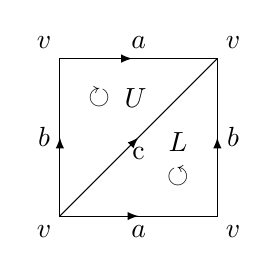
\begin{tikzpicture}
\draw[postaction={decorate},decoration={
    markings,
    mark=at position .125 with {\arrow{latex}},
    mark=at position .375 with {\arrow{latex}},
    mark=at position .635 with {\arrowreversed{latex}},
    mark=at position .875 with {\arrowreversed{latex}},
    }
  ]
    (0,0)  -- (2,0) node[midway, below] {$a$} --(2,2) node[midway, right] {$b$} --(0,2) node[midway, above] {$a$}  -- cycle node[midway, left] {$b$};
\draw[postaction={decorate},decoration={
    markings,
    mark=at position 0.5 with {\arrow{latex}}
    }
  ]
     (0,0) -- (2,2) node[midway, below] {c};
     
     
\draw (-0.2,0) node[below] {$v$};
\draw (2.2, 0) node[below] {$v$};
\draw (-0.2,2) node[above] {$v$};
\draw (2.2,2) node[above] {$v$};

\draw (0.5,1.5)  node {$\circlearrowright$};
\draw (1.5,0.5)  node {$\circlearrowleft$};

\draw (1.5,0.7) node[above] {$L$};
\draw (0.7,1.5) node[right] {$U$};
    

\end{tikzpicture}
$$
Then we have 
$$C_k^{\Delta}(\mathbb{T}^2) \cong \ \begin{cases} \ \Z v \cong \Z, & \textrm{ for }k=0, \\ \ \Z a \oplus \Z b \oplus \Z c \cong \Z^3, & \textrm{ for } k=1, \\ \ \Z U \oplus \Z L \cong \Z^2, &\textrm{ for }k=2, \\ \ 0,& \textrm{ otherwise.} \end{cases}$$
The boundaries are 
$$\partial^{\Delta}_2(U) = a+b-c. \qquad \partial^{\Delta}_2(L)=a+b-c, \qquad \partial^{\Delta}_1(a)=\partial^{\Delta}_1(b) = \partial^{\Delta}_1(c)=0,$$
i.e. we can describe them by the $\Z$-linear maps $\partial^{\Delta}_0= \partial^{\Delta}_1 = 0$ and by choosing the basis $\{U,L\}$ of $\Z^2$ and $\{a,b,c\} \in \Z^3$
$$\partial^{\Delta}_2: \Z^2 \la \Z^3, \qquad z= \begin{pmatrix} z_1 \\[-6pt] z_2\end{pmatrix} \mapsto \begin{pmatrix}[rr] 1 & 1 \\[-6pt] 1 & 1 \\[-6pt] -1 &-1 \end{pmatrix} z.$$
The simplicial chain complex now looks like 
$$ \ldots \la 0 \la \Z^2 \overset{\partial^{\Delta}_2}{\la} \Z^3 \overset{\partial^{\Delta}_1}{\la} \Z \overset{\partial^{\Delta}_0}{\la} 0 \la \ldots$$
The nontrivial kernels and images are
$$\ker \partial^{\Delta}_2 = \left\{ \begin{pmatrix}[r] -k \\[-6pt] k \end{pmatrix} \ \Bigg\vert \ k \in \Z \right\} \cong \Z,$$
$$\mathrm{im} \ \partial^{\Delta}_2 = \left\{ \begin{pmatrix}[r] k \\[-6pt] k \\[-6pt] -k \end{pmatrix}\ \Bigg \vert \ k \in \Z \right\} \cong \Z$$
which gives us
$$H_0^{\Delta}(\mathbb{T}^2) \cong \slant{\ker \partial^{\Delta}_0}{\mathrm{im} \ \partial^{\Delta}_1} \cong \slant{\Z}{0} \cong \Z,$$
$$H_1^{\Delta}(\mathbb{T}^2) \cong \slant{\ker \partial^{\Delta}_1}{\mathrm{im} \ \partial^{\Delta}_2} \cong \slant{\Z^3}{\Z} \cong \Z^2,$$
$$H_2^{\Delta}(\mathbb{T}^2) \cong \slant{\ker \partial^{\Delta}_2}{\mathrm{im} \ \partial^{\Delta}_3} \cong \slant{\Z}{0} \cong \Z.$$
Finally we obtain
$$H_k^{\Delta}(\mathbb{T}^2) \ \cong \ \begin{cases} \ \Z,& \textrm{ if }k \in \{0,2\},\\ \ \Z^2, & \textrm{ if }k=1, \\ \ 0, & \textrm{ otherwise.} \end{cases}$$

\item For the Klein bottle we proceed analogously. Consider the $\Delta$-complex structure
$$
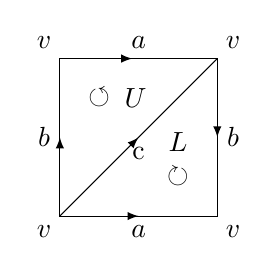
\begin{tikzpicture}
\draw[postaction={decorate},decoration={
    markings,
    mark=at position .125 with {\arrow{latex}},
    mark=at position .375 with {\arrowreversed{latex}},
    mark=at position .635 with {\arrowreversed{latex}},
    mark=at position .875 with {\arrowreversed{latex}},
    }
  ]
    (0,0)  -- (2,0) node[midway, below] {$a$} --(2,2) node[midway, right] {$b$} --(0,2) node[midway, above] {$a$}  -- cycle node[midway, left] {$b$};
\draw[postaction={decorate},decoration={
    markings,
    mark=at position 0.5 with {\arrow{latex}}
    }
  ]
     (0,0) -- (2,2) node[midway, below] {c};
     
     
\draw (-0.2,0) node[below] {$v$};
\draw (2.2, 0) node[below] {$v$};
\draw (-0.2,2) node[above] {$v$};
\draw (2.2,2) node[above] {$v$};

\draw (0.5,1.5)  node {$\circlearrowleft$};
\draw (1.5,0.5)  node {$\circlearrowright$};

\draw (1.5,0.7) node[above] {$L$};
\draw (0.7,1.5) node[right] {$U$};

\end{tikzpicture}
$$
Then we have
$$C_k^{\Delta}(K) \cong \ \begin{cases} \ \Z v \cong \Z, & \textrm{ for }k=0, \\ \ \Z a \oplus \Z b \oplus \Z c \cong \Z^3, & \textrm{ for } k=1, \\ \ \Z U \oplus \Z L \cong \Z^2, &\textrm{ for }k=2, \\ \ 0,& \textrm{ otherwise.} \end{cases}$$
The boundaries are
$$\partial_2^{\Delta}(U)= -a-b+c, \qquad \partial_2^{\Delta}(L) = -a+b+c, \qquad \partial_1^{\Delta}(a)=\partial_1^{\Delta}(b)=\partial_1^{\Delta}(c)=0,$$
i.e. we can describe them by the $\Z$-linear maps $\partial_0^{\Delta}=\partial_1^{\Delta}=0$ and by choosing the same basis as above
$$\partial^{\Delta}_2: \Z^2 \la \Z^3, \qquad z= \begin{pmatrix} z_1 \\[-6pt] z_2\end{pmatrix} \mapsto \begin{pmatrix}[rr] -1 & -1 \\[-6pt] -1 & 1 \\[-6pt] 1 &1 \end{pmatrix} z.$$
The simplicial chain complex now looks like
$$ \ldots \la 0 \la \Z^2 \overset{\partial^{\Delta}_2}{\la} \Z^3 \overset{\partial^{\Delta}_1}{\la} \Z \overset{\partial^{\Delta}_0}{\la} 0 \la \ldots$$
The only nontrivial image is
\begin{alignat*}{5}
\mathrm{im} \ \partial_2^{\Delta} \ \ &\cong&& \ \ \left\{ \begin{pmatrix}[r] -z_1 - z_2 \\[-6pt] -z_1+z_2 \\[-6pt] z_1 + z_2 \end{pmatrix} \ \Bigg\vert \ z_1, z_2 \in \Z \right\} \\
&=&& \ \ \left\{ \begin{pmatrix}[r] -k \\[-6pt] -k+2z_2 \\[-6pt] k \end{pmatrix}\ \Bigg \vert \ k,z_2 \in \Z \right\} \\
&\cong&& \ \ \left\{k \begin{pmatrix}[r] -1 \\[-6pt]-1\\[-6pt] 1 \end{pmatrix} + l \begin{pmatrix}[r]0\\[-6pt] 2 \\[-6pt] 0 \end{pmatrix} \ \Bigg \vert \ k,l \in \ \right\} \\
&\cong&& \ \ \Z \oplus 2 \Z
\end{alignat*}
(note that $\partial_2^{\Delta}$ is injective). Then we compute
$$H_0^{\Delta}(K) \cong \slant{\ker \partial_0^{\Delta}}{\mathrm{im} \ \partial_1^{\Delta}} \cong \slant{\Z}{0} \cong \Z,$$
$$H_1^{\Delta}(K) \cong \slant{\ker \partial_1^{\Delta}}{\mathrm{im} \ \partial_2^{\Delta}} \cong \slant{\Z^{3}}{\Z \oplus \Z^2} \cong \Z \oplus \slant{\Z}{2 \Z},$$
$$H_2^{\Delta}(K) \cong \slant{\ker \partial_2^{\Delta}}{\mathrm{im} \ \partial_3^{\Delta}} \cong \slant{0}{0} \cong 0.$$
Finally we obtain 
$$H_k^{\Delta}(K) \ \cong \ \begin{cases} \ \Z, & \textrm{ if k=0}, \\ \ \Z \oplus \slant{\Z}{2 \Z}, & \textrm{ if }k=1, \\ \ 0, & \textrm{ otherwise,} \end{cases}$$
which finishes the probelm. $\hfill \Box$





\end{compactenum}
\end{sol}

\end{prob}


\begin{prob}   %%AUFGABE 6.4
Let $G$ be a group with presentation $G=\langle S \ \vert \ R \rangle$ and let $X_G$ be the associated presentation complex, i.e. $\pi_1(X_G) \cong G$. Endow $X_G$ wit the structure of a $\Delta$-complex and show that $H_1^{\Delta}(X_G)$ is isomorphic to the abelianization of $G$.
\begin{sol}
$X_G$ is a wedge of $\vert S \vert$ many circles and for each relator $r=s_1^{k_1} \cdots s_n^{k_n}$ we attach a $2$-cell along the word $r$. If $r$ has length $n$, this amounts to gluing an $n$-gon with edges labeled $s_1, \ldots s_n$ to $\bigvee_{s \in S} \Sph^1$ according to the labeling. We obtain a $\Delta$-complex structure on $X_G$ as follows: In each $n$-gon coming from a relator, fix a vertex and add edges to the remaining $n-3$ vertices. Then the $\Delta$-complex structure consists of 
\begin{compactitem}
\item $0$-simplices: The base point.
\item $1$-simplices: One for each $s \in S$ and for each relator $r \in R$ of length $n$ we add $n-3$ edges.
\item $2$-simplices: For each $r \in R$ of length $n$ we have $n-2$ $2$-simplices.
\end{compactitem}
Since there is only one vertex, $\partial_1^{\Delta}=0$, so $\ker \partial_1$ is the free abelian group on the set of $1$-simplices. Now 
$$H_1^{\Delta}(X_G) = \slant{\ker \partial_1^{\Delta}}{\mathrm{im} \ \partial_2^{\Delta}}$$
and modding out $\mathrm{im} \ \partial^{\Delta}_2$ amounts to killing the $1$-simplices which do not come from $S$, and adding relations $0=\sum_{i=1}^m k_is_i$ for a relator $r=s_1^{k_1} \cdots s_m^{k_m}$. Consider the example $r=s_1^2s_2^2$:
$$
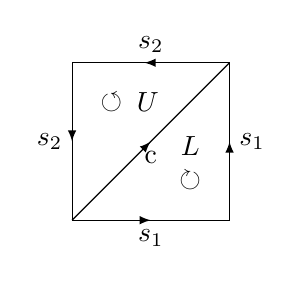
\begin{tikzpicture}
\draw[postaction={decorate},decoration={
    markings,
    mark=at position .125 with {\arrow{latex}},
    mark=at position .375 with {\arrow{latex}},
    mark=at position .635 with {\arrow{latex}},
    mark=at position .875 with {\arrow{latex}},
    }
  ]
    (0,0)  -- (2,0) node[midway, below] {$s_1$} --(2,2) node[midway, right] {$s_1$} --(0,2) node[midway, above] {$s_2$}  -- cycle node[midway, left] {$s_2$};
\draw[postaction={decorate},decoration={
    markings,
    mark=at position 0.5 with {\arrow{latex}}
    }
  ]
     (0,0) -- (2,2) node[midway, below] {c};


\draw (0.5,1.5)  node {$\circlearrowleft$};
\draw (1.5,0.5)  node {$\circlearrowright$};

\draw (1.5,0.7) node[above] {$L$};
\draw (0.7,1.5) node[right] {$U$};

\end{tikzpicture}
$$
Then 
$$\partial_2^{\Delta}(U) = a + s_2 + s_2 = 0, \qquad \partial_2^{\Delta}(L) = s_1 + s_1 - a =0,$$
i.e. $2s_1 + 2s_2 =0$. Thus we have that
$$H_1^{\Delta}(X_g) = \slant{G}{[G,G]}$$
is the abelianization of $G$. $\hfill \Box$



\end{sol}
\end{prob}




















\newpage 



\titlespacing*{\section}{-16.5pt}{0pt}{20pt}
\renewcommand*\thesection{}
\section{Problem set 7} %PARAGRAPH B.7
\renewcommand*\thesection{\arabic{section}}




\begin{prob} %%%AUFGABE 7.1
Prove or disprove the following assertions.
\begin{compactenum}
\item If the sequence of $\Z$-modules $0 \la M \la N \la \Z \la 0$ is exact, then $N \cong M \oplus \Z$.
\item If the sequence of $\Z$-modules $0 \la M \la N \la \slant{\Z}{2 \Z} \la 0$ is exact, then $N \cong M \oplus \slant{\Z}{2\Z}$.
\item If the sequence of $\slant{\Z}{2\Z}$-modules $0 \la M \la N \la \slant{\Z}{2\Z} \la 0$ is exact, then $N \cong M \oplus \slant{\Z}{2\Z}$.
\end{compactenum}
\begin{sol}
\begin{compactenum}
\item This is true. We will prove a more general lemma:
\begin{compactenum}
\item[\textbf{claim.}] Let $R$ be a ring and $0\la A \overset{i}{\la} B \overset{p}{\la} C \la 0$ be a short exact sequences of $R$-modules. Suppose there exists a homomorphisms $s: C \la B$ with $p \circ s = \id_C$. Then $B \cong A \oplus C$, i.e. the diagram
$$
\begin{xy}
\xymatrix{
0 \ar[r] & A \ar[r]^{i} \ar[rd]_{\iota} & B \ar[d]^{\cong} \ar[r]^{p} & C \ar[r] & 0 \\ && A \oplus C \ar[ru]_{\pi} &&
}
\end{xy}
$$
commutes.
\item[\textbf{proof.}] Define homomorphisms
$$\phi: A \oplus C \la B, \qquad (a,c) \mapsto i(a) +s (c),$$
$$\psi: B \la A \oplus C, \qquad b \mapsto \left(i^{-1}\left(b-s(p(b))\right), p(b)\right).$$
Note that $\psi$ is well-defined, since we have 
$$p\left( b-s(p(b))\right) = p(b) - (p \circ s)(p(b)) = p(b) - p(b) =0,$$
i.e. $b- s(p(b)) \in \ker p = \mathrm{im} \ i$. Since $i$ is injective, $b-s(p(b))$ has exactly one preimage under $i$ which we denote by $i^{-1}\left(b-s(p(b))\right)$. Noe $\phi$ and $\psi$ are inverse to each other: For $b \in B$ we have
\begin{alignat*}{5}
(\phi \circ \psi)(b) \ \  &=&& \ \ \phi \left(\left(i^{-1}( b - s(p(b))), p(b) \right)\right) \\
&=&& \ \ i \left( i^{-1}\left(b-s(p(b))\right) \right) + s(p(b)) \\
&=&& \ \ b- s(p(b)) + s(p(b)) \\
&=&& \ \ b
\end{alignat*}
and for $(a,c) \in A \oplus C$ we see
\begin{alignat*}{5}
(\psi \circ \phi)(a,c) \ \ &=&& \ \ \psi\left( i(a) + s(c)\right) \\
&=&& \ \ \left( i^{-1}\left(i(a)+s(c)-s\left(p(i(a)+s(c))\right) \right), p(i(a)+s(c)) \right) \\
&=&& \ \ \left( a + i^{-1}(s(c)) - i^{-1}(s(p(i(a)))) + i^{-1}(s(p(s(c)))), p(i(a)) + p(s(c)) \right) \\
&=&& \ \ \left( a + i^{-1}(s(c)) -i^{-1}(0) + i^{-1}(s(c)), c \right) \\
&=&& \ \ \left( a,c \right)
\end{alignat*}
where we used that $p \circ s = \id_C$ and $p \circ i=0$. Thus $B \cong A \oplus C$.
\end{compactenum}
To show that (i) is true, we need to find a split $s: \Z \la N$. Since $p: N \la \Z$ is surjective, there exists $n \in N$ with $p(n) = 1$. Then define $s$ by $s(1)=n$. Then for any $z \in \Z$ we have 
$$(p \circ s)(z) = p(s(z)) = p(zs(1)) =p(zn)=z p(n) = z,$$
hence $s$ is a split and by the lemma we have $N \cong M \oplus \Z$. 

\item This not true. Consider the sequence
$$0 \la \Z \xrightarrow[z \mapsto 2z]{i} \Z \xrightarrow[z \mapsto \overline{z}]{p} \slant{\Z}{2 \Z} \la 0$$
Then $\alpha$ is injective, $\pi$ is surjective and $\ker \pi = 2 \Z = \mathrm{im} \ \alpha$, i.e. the sequence is exact. However $\Z \ncong \Z \oplus \slant{\Z}{2\Z}$. 
\item The dimension formula for vector space of $\slant{\Z}{2\Z}$ gives us
$$N \cong \ker p \oplus \mathrm{im} \ p \cong \mathrm{im} \ i \oplus \mathrm{im} \ p \cong M \oplus \slant{\Z}{2\Z}.$$
Alternatively define the split $s: \slant{\Z}{2\Z} \la N$ by $s(1)=n_0$ for some $n_0 \in p^{-1}(\{1\})$.

$\hfill \Box$

\end{compactenum}

\end{sol}

\end{prob}


\begin{prob}   %%AUFGABE 7.2
Consider the $\Delta$-complex $K$ given by
$$
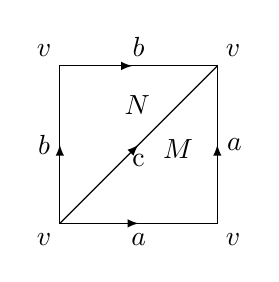
\begin{tikzpicture}
\draw[postaction={decorate},decoration={
    markings,
    mark=at position .125 with {\arrow{latex}},
    mark=at position .375 with {\arrow{latex}},
    mark=at position .635 with {\arrowreversed{latex}},
    mark=at position .875 with {\arrowreversed{latex}},
    }
  ]
    (0,0)  -- (2,0) node[midway, below] {$a$} --(2,2) node[midway, right] {$a$} --(0,2) node[midway, above] {$b$}  -- cycle node[midway, left] {$b$};
\draw[postaction={decorate},decoration={
    markings,
    mark=at position 0.5 with {\arrow{latex}}
    }
  ]
     (0,0) -- (2,2) node[midway, below] {c};
     
     
\draw (-0.2,0) node[below] {$v$};
\draw (2.2, 0) node[below] {$v$};
\draw (-0.2,2) node[above] {$v$};
\draw (2.2,2) node[above] {$v$};


\draw (1.5,0.7) node[above] {$M$};
\draw (0.7,1.5) node[right] {$N$};

\end{tikzpicture}
$$
\begin{compactenum}
\item Explain that $K$ is the Klein bottle and that the subcomplex given by the $2$-simplex $M$ and its subsimplices is an embedded Möbius strip.
\item Compute the absolute and relative simplicial homology $H_*^{\Delta}(M;R)$, $H_*^{\Delta}(K;R)$ and $H_*^{\Delta}(K,M;R)$ for $R= \Z$.
\item Do the same as in (ii) for $R=\slant{\Z}{2\Z}$.
\item Your results make the objects in the long exact sequence of the $\Delta$-pair $(K,M)$ explicit. Find all homomorphisms for both coefficient rings.

\end{compactenum}

\begin{sol}
\begin{compactenum}
\item We have 
$$
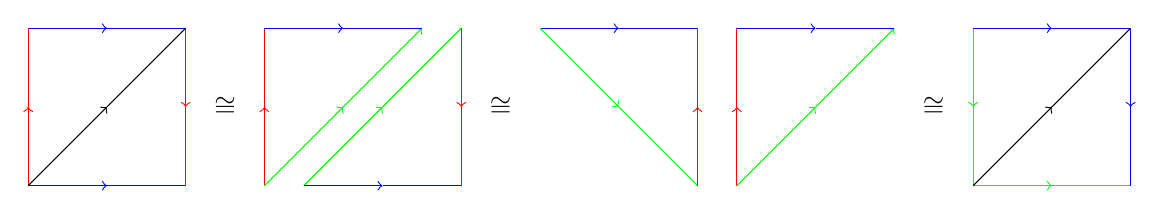
\begin{tikzpicture}
\draw[->,color=blue] (1,0) --(2,0);
\draw[color=blue] (1,0) -- (3,0);
\draw[color=blue,->] (1,2) -- (2,2);
\draw[color=blue] (2,2) -- (3,2);
\draw[color=red,->] (3,2) -- (3,1);
\draw[color=red] (3,1) -- (3,0);
\draw[color=red,->] (1,0) -- (1,1);
\draw[color=red] (1,1) -- (1,2);
\draw[->] (1,0) -- (2,1);
\draw (2,1) -- (3,2);

\draw (3.5,1) node {$\cong$};

\draw[color=red,->] (4,0) -- (4,1);
\draw[color=red] (4,1) -- (4,2);
\draw[color=green,->] (4,0) -- (5,1);
\draw[color=green,->] (5,1) -- (6,2);
\draw[color=blue,->] (4,2) -- (5,2);
\draw[color=blue] (5,2) -- (6,2);

\draw[color=green,->] (4.5,0) -- (5.5,1);
\draw[color=green] (5.5,1) -- (6.5,2);
\draw[color=blue,->] (4.5,0) -- (5.5,0);
\draw[color=blue] (5.5,0) -- (6.5,0);
\draw[color=red,->] (6.5,2) -- (6.5,1);
\draw[color=red] (6.5,1) -- (6.5,0);

\draw (7,1) node {$\cong$};

\draw[color=blue,->] (7.5,2) -- (8.5,2);
\draw[color=blue] (8.5,2) -- (9.5,2);
\draw[color=green,->] (7.5,2) -- (8.5,1);
\draw[color=green] (8.5,1) -- (9.5,0);
\draw[color=red,->] (9.5,0) -- (9.5,1);
\draw[color=red] (9.5,1) -- (9.5,2);

\draw[color=red,->] (10,0) -- (10,1);
\draw[color=red] (10,1) -- (10,2);
\draw[color=green,->] (10,0) -- (11,1);
\draw[color=green,->] (11,1) -- (12,2);
\draw[color=blue,->] (10,2) -- (11,2);
\draw[color=blue] (11,2) -- (12,2);

\draw (12.5,1) node{$\cong$};

\draw[color=green,->] (13,2) -- (13,1);
\draw[color=green] (13,1) -- (13,0);
\draw[color=green,->] (13,0) -- (14,0);
\draw[color=green] (14,0) -- (15,0);
\draw[color=blue,->] (13,2) -- (14,2);
\draw[color=blue] (14,2) -- (15,2);
\draw[color=blue,->] (15,2) -- (15,1);
\draw[color=blue] (15,1) -- (15,0);
\draw[->] (13,0) -- (14,1);
\draw (14,1) -- (15,2);

\end{tikzpicture}
$$

where the left image is the usual presentation of $K$ and the right one the image from the problem. Further we have seen in problem 6.20 that $M$ corresponds to the Möbius strip.


\item In problem 6.22 we have seen that
$$C_k^{\Delta}(K;\Z) \cong \ \begin{cases} \ \Z v \cong \Z, & \textrm{ for }k=0, \\ \ \Z a \oplus \Z b \oplus \Z c \cong \Z^3, & \textrm{ for } k=1, \\ \ \Z U \oplus \Z L \cong \Z^2, &\textrm{ for }k=2, \\ \ 0,& \textrm{ otherwise.} \end{cases}$$
and 
$$H_k^{\Delta}(K;\Z) \ \cong \ \begin{cases} \ \Z & \textrm{ if k}=0, \\ \ \Z \oplus \slant{\Z}{2 \Z} & \textrm{ if }k=1, \\ \ 0 & \textrm{ otherwise.} \end{cases}$$
For the chain complex for $M$ we have 
$$C_k^{\Delta}(M;\Z) \cong \ \begin{cases} \ \Z v \cong \Z & \textrm{ for }k=0,\\ \ \Z a \oplus \Z c \cong \Z^2 & \textrm{ for }k=1, \\ \ \Z M \cong \Z & \textrm{ for } k=2,\\ \ 0 & \textrm{ otherwise} \end{cases}$$
with boundaries $\partial_1^{\Delta}=0= \partial_0^{\Delta}$. Now $\partial_2^{\Delta}(M) = 2a-c$, i.e. we can describe $\partial_2^{\Delta}$ as the injective $\Z$-linear map 
$$\partial_2^{\Delta}: \Z \la \Z^2, \qquad z \mapsto \begin{pmatrix}2z\\[-6pt] -z \end{pmatrix}.$$
Then the simplicial chain complex for $M$ looks like 
$$ \ldots \la 0 \la \Z \overset{\partial^{\Delta}_2}{\la} \Z^2 \overset{\partial^{\Delta}_1}{\la} \Z \overset{\partial^{\Delta}_0}{\la} 0 \la \ldots$$
The only nontrivial image of the boundaries is
$$\mathrm{im} \ \partial_2^{\Delta} = \left\{ \begin{pmatrix} 2z \\[-6pt] -z \end{pmatrix} \ \Bigg\vert \ k \in \Z \right\} \cong \Z.$$
Thus we have 
$$H_0^{\Delta}(M;\Z) \cong \ \slant{\ker \partial_0^{\Delta}}{\mathrm{im}\ \partial_1^{\Delta}} \cong {\Z}{0} \cong \Z,$$
$$H_1^{\Delta}(M;\Z) \cong \ \slant{\ker \partial_1^{\Delta}}{\mathrm{im}\ \partial_2^{\Delta}} \cong {\Z^2}{\Z} \cong \Z,$$
$$H_2^{\Delta}(M;\Z) \cong \ \slant{\ker \partial_2^{\Delta}}{\mathrm{im}\ \partial_3^{\Delta}} \cong {0}{0} \cong 0,$$
i.e. 
$$H_k^{\Delta}(M;\Z) \ \cong \ \begin{cases} \ \Z & \textrm{ if } k\in \{0,1\}, \\  \ 0 & \textrm{ otherwise.} \end{cases}$$
For the relative simplicial homology groups consider the chain modules
$$C_k^{\Delta}(K,M;\Z) \ \cong \ \slant{C_k^{\Delta}(K;\Z)}{C_k^{\Delta}(M;\Z)} \ \cong \ \begin{cases} \ \Z & \textrm{ for } k \in \{1,2\}, \\ \ 0 & \textrm{ otherwise. } \end{cases}$$
The boundary map $\partial_2^{\Delta}$ descends from 
$$\partial_2^{\Delta}: \Z^2 \la \Z^3, \qquad z=\begin{pmatrix}[r] z_1 \\[-6pt]z_2\end{pmatrix} \mapsto \begin{pmatrix}[rr]2 & 0 \\[-6pt] 0 & 2 \\[-6pt] -1 & -1 \end{pmatrix} z$$
(with basis $\{M,N\}$ on the left and $\{a,b,c\}$ on the right) to 
$$\partial_2^{\Delta}: \Z \cong \Z M \cong \la \Z b \cong \Z, \qquad N \mapsto 2b$$
(note that any simplices in $M$ are now zero).Thus $\partial_2^{\Delta}$ is injective with
$$\mathrm{im} \ \partial_2^{\Delta} \cong  2 \Z$$
and we see
$$H_k^{\Delta}(K,M;\Z) \ \cong \ \begin{cases} \ \slant{\Z}{2\Z} & \textrm{ if }k=1, \\ \ 0 & \textrm{ otherwise. } \end{cases}$$

\item Write $R:= \slant{\Z}{2\Z}$. Nothing changes for $K$ except of $\partial_2^{\Delta}$ which now is the map
$$\partial_2^{\Delta}: R^2 \la R^3, \qquad r=\begin{pmatrix}[r] r_1 \\[-6pt] r_2 \end{pmatrix} \mapsto \begin{pmatrix}[rr] -1 & -1 \\[-6pt] -1 & 1 \\[-6pt] 1 & 1 \end{pmatrix} r = \begin{pmatrix}[rr] 1 & 1 \\[-6pt] 1 & 1 \\[-6pt] 1 & 1 \end{pmatrix} r.$$
Then $\partial_2^{\Delta}$ is not injective any more and we have 
$$\ker \partial_2^{\Delta} \cong R, \qquad \mathrm{im} \ \partial_2^{\Delta} \cong R$$
and thus 
$$H_k^{\Delta}(K;R) \ \cong \ \begin{cases} \ R & \textrm{ if } k \in \{0,2\}, \\ \ R^2 & \textrm{ if }k=1, \\ 0 & \textrm{ otherwise.} \end{cases}$$
For $M$ nothing changes, except of $\partial_2^{Delta}$, which does not have any impact on kernel or image. Thus we see
$$H_k^{\Delta}(M;R) \ \cong \ \begin{cases} \ R & \textrm{ if } k \in \{0,1\} ,\\ \ 0 & \textrm{ otherwise.} \end{cases}$$
Now the relative chain modules are the same as in (ii). The difference lies in the map $\partial_2^{\Delta}$, which now is the zero map, i.e the chain complex looks like 
$$\ldots \la 0 \la R^{(2)} \overset{0}{\la} R^{(1)} \la 0 \la \ldots$$
This gives us 
$$H_k^{\Delta}(K,M;R) \ \cong \ \begin{cases} \ R & \textrm{ if } k\in \{1,2\}, \\ \ 0 & \textrm{ otherwise.} \end{cases} $$

\item For $R=\Z$ the long exact sequence is
$$\ldots \la 0  \overset{\partial_2}{\la} 0  \la 0 \la  0 \overset{\partial_1}{\la} \Z \la \Z \oplus \slant{\Z}{2\Z} \la \slant{\Z}{2\Z} \overset{\partial_0}{\la} \Z \la \Z \la 0 \la \ldots$$
and for $R= \slant{\Z}{2\Z}$ it is
$$\ldots 0 \overset{\partial_2}{\la} 0 \la R \la R \overset{\partial_1}{\la} R \la R^2 \la R \overset{\partial_0}{\la} R \la R \la 0 \la \ldots $$
By writing down generators for the modules one easily sees what happens. $\hfill \Box$
\end{compactenum}

\end{sol}

\end{prob}


\begin{prob}
Let $(H_*, \partial_*)$ be a homology theory with values in $\Rmod$. Let $(X,A)$ be a pair of spaces and suppose that $X$ retracts onto $A$. Show that the component at $(X,A)$ of the natural transformation $\partial_n$ is trivial for all $n \in \mathbb{Z}$.
\begin{sol}
Let $p: X \la A$ be continuous with $p\vert_A = \id_A$ and $i: A \hookrightarrow X$ the inclusion. Then the long exact sequence of the pair $(X,A)$ is
$$\ldots \la H_{n}(X,A;R) \overset{\partial_{n}}{\la} H_{n-1}(A;R) \overset{H_{n-1}(i)}{\la} H_{n-1}(X;R) \la H_{n-1}(X,A;R) \la \ldots$$
Now $H_{n-1}(i)$ has a left inverse $H_{n-1}(r)$, since
$$H_{n-1}(r) \circ H_{n-1}(i) = H_{n-1}(r \circ i) = H_{n-1}(\id_A) = \id_{H_{n-1}(A)},$$
thus $H_{n-1}(i)$ must be injective. But then by exactness $0=\ker H_{n-1}(i) = \mathrm{im} \ \partial_n$, i.e. the boundaries all trivial, which was to be shown. $\hfill \Box$

\end{sol}
\end{prob}



























\newpage 



\titlespacing*{\section}{-16.5pt}{0pt}{20pt}
\renewcommand*\thesection{}
\section{Problem set 8} %PARAGRAPH B.8
\renewcommand*\thesection{\arabic{section}}





\begin{prob} %%AUFGABE 8.1
Let $R$ be a ring and $0 \la A \overset{i}{\la} B \overset{j}{\la} C \la 0$ be a short exact sequence of $R$-modules.
\begin{compactenum}
\item Show that the following three statements are equivalent:
\begin{compactenum}
\item There is a homomorphism $p:B \la A$ such that $p \circ i = \id_A$.
\item There is a homomorphism $s: C \la B$ such that $j \circ s = \id_C$.
\item There is an isomorphism $\phi: B \la A\oplus C$ fitting into the diagram
$$
\begin{xy}
\xymatrix{
&&B \ar[dd]^{\phi} \ar[rd]^{j} &&\\
0 \ar[r] & A \ar[ru]^{i} \ar[rd] && C \ar[r] & 0 \\
&& A \oplus C \ar[ru] &&
}
\end{xy}
$$
where the lower arrows are given by $a \mapsto (a,0)$ and $(a,c) \mapsto c$.

\end{compactenum}
\item The sequence is called \textit{split}, if it satisfies one and thus any of the above conditions. Show that the short exact sequence always splits if $C$ is a free $R$-module.
\item Suppose $R$ is a principal ideal domain (e.g. $R=\Z$). Show that if every short exact sequence as above splits, then $C$ is free.
\end{compactenum}

\begin{sol}
\begin{compactenum}
\item This is a more general version of the lemma in problem 7.24.
\begin{compactenum}
\item["$(1)\Rightarrow (3)$"] Let $p: B \la A$ be an $R$-linear map satisfying $p \circ i = \id_A$ and define
$$\phi: B \la A \oplus C, \qquad b \mapsto (p(b), j(b)).$$
Then for $b \in \ker \phi$ we have $p(b)=j(b)=0$. Since $\ker j = \mathrm{im} \ i$, we can write $b=i(a)$for some $a \in A$. But then $0=p(b)=p(i(a))=a$ implies $b=i(a)=i(0)=0$, i.e. $\phi$ is injective. For surjectivity consider $(a,c) \in A \oplus C$. Since $j$ is surjective, write $c=j(\tilde{b})$ for some $\tilde{b}\in B$. Then for $b:= \tilde{b}+i(a-p(\tilde{b}))$ we obtain 
\begin{alignat*}{5}
\phi(b) \ \ &=&& \ \ \phi(\tilde{b} + i(a-p(\tilde{b})) \\
&=&& \ \ \left( p\left(\tilde{b} + i(a-p(\tilde{b}))\right), j\left(\tilde{b} + i(a-p(\tilde{b}))\right) \right) \\
&=&& \ \ \left( p(\tilde{b} + a - p(\tilde{b}) , j(\tilde{b})\right) \\
&=&& \ \ (a,c),
\end{alignat*}
hence $\phi$ is bijective and therefore an isomorphism of groups. Now the diagram in (3) clearly commutes: for any $a \in A$ and $b \in B$ we have 
$$(\phi \circ i)(a) = \left( p(i(a)), j(i(a))\right) = (a,0), \qquad (\mathrm{pr}_C \circ \phi)(b) = \mathrm{pr}_C(p(b), j(b)) =j(b).$$

\item["$(2)\Rightarrow(3)$"] Let now $s: C \la B$ with $j \circ s = \id_C$. Then the map
$$\phi: B \la A \oplus C, \qquad b \mapsto \left( i^{-1}\left( b- s(j(b))\right), j(b)\right)$$
is $R$-linear with inverse 
$$\psi: A \oplus C \la B, \qquad (a,c) \mapsto i(a) + s(c).$$
Indeed for $b \in B$ we have 
\begin{alignat*}{5}
(\psi \circ \phi)(b) \ \  &=&& \ \ \psi \left(\left(i^{-1}( b - s(p(b))), p(b) \right)\right) \\
&=&& \ \ i \left( i^{-1}\left(b-s(p(b))\right) \right) + s(p(b)) \\
&=&& \ \ b- s(p(b)) + s(p(b)) \\
&=&& \ \ b
\end{alignat*}
and for $(a,c) \in A \oplus C$ we see
\begin{alignat*}{5}
(\phi \circ \psi)(a,c) \ \ &=&& \ \ \phi\left( i(a) + s(c)\right) \\
&=&& \ \ \left( i^{-1}\left(i(a)+s(c)-s\left(p(i(a)+s(c))\right) \right), p(i(a)+s(c)) \right) \\
&=&& \ \ \left( a + i^{-1}(s(c)) - i^{-1}(s(p(i(a)))) + i^{-1}(s(p(s(c)))), p(i(a)) + p(s(c)) \right) \\
&=&& \ \ \left( a + i^{-1}(s(c)) -i^{-1}(0) + i^{-1}(s(c)), c \right) \\
&=&& \ \ \left( a,c \right).
\end{alignat*}
Again the diagram in (3) commutes: For $a \in A$ and $b\in B$ we have 
$$(\phi \circ i)(a) = \left( i^{-1}\left(i(a) - s(j(i(a)))\right), j(i(a))\right) = (a,0)$$
and
$$(\mathrm{pr}_C \circ \phi)(b) = \mathrm{pr}_C\left(i^{-1}\left( b - s(j(b))\right), j(b)\right) = j(b).$$
\item["$(3)\Rightarrow(2)$"] Define
$$s: C \la B, \qquad c \mapsto (\phi^{-1}\circ \iota)(c),$$
where $\iota: C \la A \oplus C$ denotes the inclusion. Then we have 
$$(j \circ s)(c) = (j \circ \phi^{-1} \circ \iota)(c) = c$$
by commutativity of the diagram in (3).
\item["$(3)\Rightarrow(1)$"] Similarly define
$$p: B \la A, \qquad b \mapsto (\mathrm{pr}_A\circ \phi)(b).$$
Then again
$$(p \circ i)(a) = (\mathrm{pr}_A \circ \phi \circ i)(a) = a,$$
hence $p \circ i = \id_A$.
\end{compactenum}
\item Let $C$ be free with basis $\{c_i\}_{i \in I}$. Since $j$ is surjective we may find $b_i \in B$ with $c_i = j(b_i)$ for all $i \in I$. Then define $s: C \la B$ by $s(c_i) = b_i$. Obviously $(j \circ s)(c_i) = c_i$ for all $i \in I$, thus $j \circ s = \id_C$ and the sequence splits.

\item For any $R$-module $C$ let $F(C)$ denote the free $R$-module with basis $C$ and consider the short exact sequence
$$0 \la \ker p \overset{i}{\la} F(C) \overset{p}{\la} C \la 0.$$
Then by assumption the sequence splits, so that we obtain $F(C) \cong \ker p \oplus C$.Then we may consider $C$ as a submodule of $F(C)$ and since $C$ is a prinicipal ideal domain, submodules of free modules are free and thus $C$ is free, which we wanted to show. $\hfill \Box$
\end{compactenum}

\end{sol}

\end{prob}

\begin{prob}    %%AUFGABE 8.2
Let $(C_*,c_*)$ and $(D_*,d_*)$ be two chain complexes o $R$-modules. Show that chain homotopy defines an equivalence relation on the set of chain maps $f_* (C_*,c_*) \la (D_*,d_*)$.
\begin{sol}
Recall that two chain maps $f_*, g_*: (C_*,c_*) \la (D_*,d_*)$ are homotopic if there exists a family $\{h_n: C_n \la D_{n+1}\}_{n \in \Z}=:h_*$ of homomorphisms, such that 
$$f_n - g_n = h_{n-1} \circ c_n + d_n \circ h_n$$
for all $n \in \Z$.
\begin{compactitem}
\item \textit{reflexivity.} Let $f_*: (C_*,c_*) \la (D_*,d_*)$ be any chain map. Then or $h_n:=0$ for all $n \in \Z$ we obtain 
$$0=f_n-f_n= h_{n-1} \circ c_n + d_{n+1}\circ h_n,$$
i.e. $f_* \sim_{h_*} f_*$.
\item \textit{symmetry.} Assume $f_*, g_*: (C_*,c_*) \la (D_*,d_*)$ are chain maps and there is a chain homotopy $f_* \sim_{h_*} g_*$, i.e. we have $f_n - g_n = h_{n-1} \circ c_n + d_{n+1} \circ h_n$ for all $n\in \Z$. Then for $\tilde{h}_* := -h_*$ we have
\begin{alignat*}{5} g_n - f_n = -(f_n - g_n) \ &=&& \  -(h_{n-1} \circ c_n + d_{n+1} \circ h_n) \\
&=&& \ (-h_{n-1}) \circ c_n  + d_{n+1} \circ (-h_n)\\
& =&& \ \tilde{h}_{n+1} \circ c_n + d_{n+1} \circ \tilde{h}_n,
\end{alignat*}
i.e. $g_* \sim_{\tilde{h}_*} f_*$. 
\item \textit{transitivity.} Let $f_*,g_*,k_*: (C_*,c_*) \la (D_*,d_*)$ be chain maps such that $f_* \sim_{h_*^1} g_*$ and $g_* \sim_{h_*^2} k_*$. Then 
\begin{alignat*}{5}
f_n - k_n  \ \ &=&& \ \ (f_n - g_n) +(g_n - k_n) \\
&=&& \ \ h_{n-1}^1 \circ c_n + d_{n+1} \circ h_n^1 + h_{n-1}^2 \circ c_n + d_{n+1} \circ h_n^2 \\
&=&& \ \ (h_{n-1}^1 + h_{n-1}^2) \circ c_n + d_{n+1} \circ (h_n^1 + h_n^2) \\
&=&& \ \ \tilde{h}_{n-1} \circ c_n + d_{n+1}\circ \tilde{h}_n
\end{alignat*}
with the chain homotopy $h\tilde{h}_* = h_*^1 + h_*^2$. Thus the claim is proved. $\hfill \Box$


\end{compactitem}


\end{sol}
\end{prob}


\begin{prob}   %%AUFGAB 8.3
Let $X$ be a $\Delta$-complex. 
\begin{compactenum}
\item Show that the first barycentric subdivision of $X$ produces a $\Delta$-complex in which each simplex has all its vertices distinct. 
\item Show that another barycentric subdivision turns $X$ into a simplicial complex. 
\end{compactenum}
\begin{sol}
\begin{compactenum}
\item By induction on the dimension of the simplices in $B_1(X)$, the barycentric subdivision of $X$.
\begin{compactenum}
\item[\textbf{$n=0.$}] Clear.
\item[\textbf{$n\geqslant1.$}] Now suppose that all $(n-1)$-simplices in $B_1(X)$ have distinct vertices and let $\sigma$ be an $n$-simplex in $B_1(X)$. 
$$
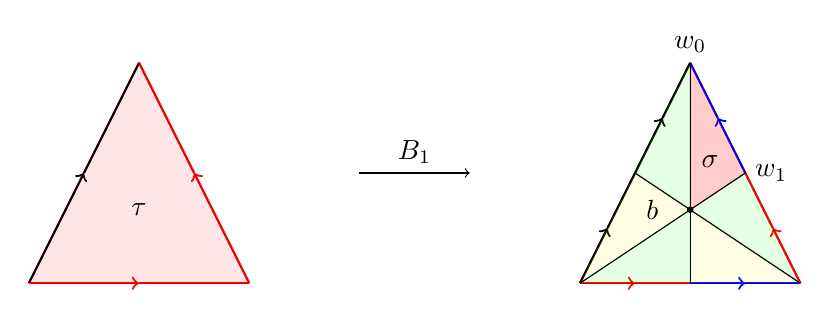
\begin{tikzpicture}[scale=1.4]
\draw[thick,->] (0,0) -- (0.5,1);
\draw[thick] (0.5,1) -- (1,2);
\draw[thick,color=red,->] (0,0) -- (1,0);
\draw[thick,color=red] (1,0) -- (2,0);
\draw[thick,color=red,->] (2,0) -- (1.5,1);
\draw[thick,color=red] (1.5,1) -- (1,2);
\draw[fill=red,opacity=0.1] (0,0) -- (2,0) -- (1,2) -- (0,0);
\draw (1,0.666666) node {$\tau$};

\draw[->] (3,1) -- (4,1);
\draw (3.5,1) node[above] {$B_1$};
\draw[thick,color=red,->] (5,0) -- (5.5,0);
\draw[thick,color=red] (5.5,0) -- (6,0);
\draw[thick,color=blue,->] (6,0) -- (6.5,0);
\draw[thick, color=blue] (6.5,0) -- (7,0);
\draw[thick,color=red,->] (7,0) -- (6.75,0.5);
\draw[thick,color=red] (6.75,0.5) -- (6.5,1);
\draw[thick,color=blue,->] (6.5,1) -- (6.25,1.5);
\draw[thick,color=blue] (6.25,1.5) -- (6,2);
\draw[thick,->] (5,0) -- (5.25,0.5);
\draw[thick] (5.25,0.5) -- (5.5,1);
\draw[thick,->] (5.5,1) -- (5.75,1.5);
\draw[thick] (5.75,1.5) -- (6,2);
\draw[fill=green,opacity=0.1] (5,0) -- (6,0) -- (6,0.6666) -- (5,0);
\draw[fill=green,opacity=0.1] (6,2) -- (6,0.66666) -- (5.5,1) -- (6,2);
\draw[fill=green,opacity=0.1] (6,0.66666) -- (6.5,1) -- (7,0) -- (6,0.66666);
\draw[fill=yellow,opacity=0.1] (5,0) -- (6,0.66666) -- (5.5,1) -- (5,0);
\draw[fill=yellow,opacity=0.1] (6,0) -- (7,0) -- (6,0.66666) -- (6,0);
\draw[fill=red,opacity=0.2] (6,2) -- (6,0.66666) -- (6.5,1) -- (6,2);
\draw (6.18,1.1) node {$\sigma$};
\draw (6,0) -- (6,2);
\draw (7,0) -- (5.5,1);
\draw (5,0) -- (6.5,1);
\draw (6,2) node[above] {$w_0$};
\draw (6.5,1) node[right] {$w_1$};
\draw (5.8,0.66666) node[left] {$b$};
\draw[fill=black] (6.025,0.666666) arc(0:360:0.025);

\end{tikzpicture}
$$
Let $\sigma$ have vertices $b,w_0,w_1, \ldots, w_{n-1}$, where $b$ is the barycenter of an $n$-simplex $\tau$ in $X$ and $[w_0, \ldots, w_{n-1}]$ is an $(n-1)$-simplex in the subdivision of a face of $\tau$. By induction hypothesis we have $w_i \neq w_j$ for all $i,j \in \{0,\ldots, n-1\}$, $i\neq j$. Now $b$ is contained in the interios of $\tau$ in $X$, thus it cannot be equal to any $w_i$. Hence all vertices $b,w_0, \ldots w_{n-1}$ are distinct.


\end{compactenum}
\item We now show that for a $\Delta$-complex in which each subcomplex has distinct vertices, the barycentric subdivision $B_1(X)$ is a simplicial complex. Note that $B_1(X)$ as above is no simplicial complex, since the two lower green triangles have the same vertices but are disctinct. Another barycentric subdivision of $X$ gives us 

$$
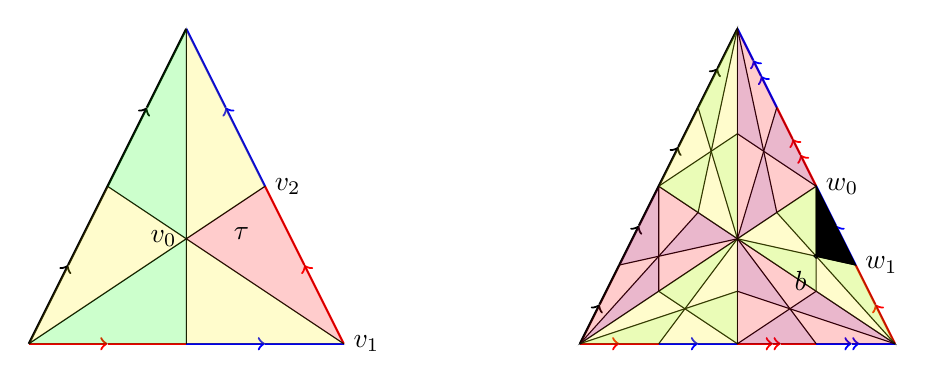
\begin{tikzpicture}

\draw[thick,color=red,->] (-7,0) -- (-6,0);
\draw[thick,color=red] (-6,0) -- (-5,0);
\draw[color=blue,->,thick] (-5,0) -- (-4,0);
\draw[color=blue,thick] (-4,0) -- (-3,0);
\draw[color=red,thick,->] (-3,0) -- (-3.5,1);
\draw[thick,color=red] (-3.5,1) -- (-4,2);
\draw[color=blue,thick,->] (-4,2) -- (-4.5,3);
\draw[color=blue,thick] (-4.5,3) -- (-5,4);
\draw[thick,->] (-7,0) -- (-6.5,1);
\draw[thick,->] (-6.5,1) -- (-5.5,3);
\draw[thick] (-5.5,3) -- (-5,4);
\draw (-7,0) -- (-4,2);
\draw (-3,0) -- (-6,2);
\draw (-5,0) -- (-5,4);
\draw[fill=green,opacity=0.2] (-7,0) -- (-5,0) -- (-5,1.3333) -- (-7,0);
\draw[fill=green,opacity=0.2] (-6,2) -- (-5,4) -- (-5,1.3333) -- (-6,2);
\draw[fill=yellow,opacity=0.2] (-7,0) -- (-5,1.3333) -- (-6,2) -- (-7,0);
\draw[fill=yellow,opacity=0.2] (-5,0) -- (-3,0) -- (-5,1.3333) -- (-5,0);
\draw[fill=yellow,opacity=0.2] (-5,4) -- (-4,2) -- (-5,1.3333) -- (-5,4);
\draw[fill=red,opacity=0.2] (-5,1.3333) -- (-3,0) -- (-4,2) -- (-5,1.3333);
\draw (-4.3,1.4) node {$\tau$};
\draw (-3,0) node[right] {$v_1$};
\draw (-4,2) node[right] {$v_2$};
\draw (-5,1.3333) node[left] {$v_0$};



\draw[thick,color=red,->] (0,0) -- (0.5,0);
\draw[thick,color=red] (0.5,0) -- (1,0);
\draw[thick,color=blue,->] (1,0) -- (1.5,0);
\draw[thick,color=blue] (1.5,0) -- (2,0);
\draw[thick,color=red,->] (2,0) -- (2.45,0);
\draw[thick,color=red,->] (2.45,0) -- (2.55,0);
\draw[thick,color=red] (2.55,0) -- (3,0);
\draw[thick,color=blue,->] (3,0) -- (3.45,0);
\draw[thick,color=blue,->] (3.45,0) -- (3.55,0);
\draw[thick,color=blue] (3.55,0) -- (4,0);

\draw[thick,color=red,->] (4,0) -- (3.75,0.5);
\draw[thick,color=red,] (3.75,0.5) -- (3.5,1);
\draw[thick,color=blue,->] (3.5,1) -- (3.25,1.5);
\draw[thick,color=blue] (3.25,1.5) -- (3,2);
\draw[thick,color=red,->] (3,2) -- (2.8,2.4);
\draw[thick,color=red,->] (2.8,2.4) -- (2.7,2.6);
\draw[thick,color=red] (2.7,2.6) -- (2.5,3);
\draw[thick,color=blue,->] (2.5,3) -- (2.3,3.4);
\draw[thick,color=blue,->] (2.3,3.4) -- (2.2,3.6);
\draw[thick,color=blue] (2.2,3.6) -- (2,4);
\draw[thick,->] (0,0) -- (0.25,0.5);
\draw[thick] (0.25,0.5) -- (0.5,1);
\draw[thick,->] (0.5,1) -- (0.75,1.5);
\draw[thick] (0.75,1.5) -- (1,2);
\draw[thick,->] (1,2) -- (1.25,2.5);
\draw[thick] (1.25,2.5) -- (1.5,3);
\draw[thick,->] (1.5,3) -- (1.75,3.5);
\draw[thick] (1.75,3.5) -- (2,4);
\draw (0,0) -- (3,2);
\draw (4,0) -- (1,2);
\draw (2,4) -- (2,0);
\draw[thin] (3,2) -- (2,2.6666) -- (1,2);
\draw[thin] (1,2) -- (1,0.6666) -- (2,0) -- (3,0.6666) -- (3,2);
\draw[thin] (0.5,1) -- (2,1.3333) -- (3.5,1);
\draw[thin] (1,0) -- (2,1.3333) -- (3,0);
\draw[thin] (1.5,3) -- (2,1.3333) -- (2.5,3);
\draw (2.5,1.6666) -- (2,4) -- (1.5,1.6666);
\draw (1.5,1.6666) -- (0,0) -- (2,0.6666) -- (4,0) -- (2.5,1.6666);

\draw[fill=green,opacity=0.1] (0,0) -- (1,0) --  (1.3333,0.4444) -- (0,0);
\draw[fill=green,opacity=0.1] (2,0) -- (1.3333,0.4444) -- (2,0.6666) -- (2,0);
\draw[fill=green,opacity=0.1] (1,0.6666) -- (2,1.3333) -- (1.3333,0.4444) -- (1,0.6666);
\draw[fill=blue,opacity=0.1] (2,0) -- (3,0) -- (2.6666,0.4444) -- (2,0);
\draw[fill=blue,opacity=0.1] (4,0) -- (2.6666,0.4444) -- (3,0.6666) -- (4,0);
\draw[fill=blue,opacity=0.1] (2,1.3333) -- (2.6666,0.4444) -- (2,0.6666) -- (2,1.3333);
\draw[fill=green,opacity=0.1] (2,1.3333) -- (3,0.6666) -- (3,1.1111) -- (2,1.3333);
\draw[fill=green,opacity=0.1] (3,1.1111) -- (2.5,1.6666) -- (3,2) -- (3,1.1111);
\draw[fill=green,opacity=0.1] (3,1.1111) -- (3.5,1) -- (4,0) -- (3,1.1111);
\draw[fill=blue,opacity=0.1] (2.3333,2.4444) -- (2,1.3333) -- (2.5,1.6666) -- (2.3333,2.4444);
\draw[fill=blue,opacity=0.1] (2.3333,2.4444) -- (3,2) -- (2.5,3) -- (2.3333,2.4444);
\draw[fill=blue,opacity=0.1] (2.3333,2.4444) -- (2,4) -- (2,2.6666) -- (2.3333,2.4444);
\draw[fill=green,opacity=0.1] (1.6666,2.4444) -- (2,2.6666) -- (2,1.3333) -- (1.6666,2.4444);
\draw[fill=green,opacity=0.1] (1.6666,2.4444) -- (2,4) -- (1.5,3) -- (1.6666,2.4444);
\draw[fill=green,opacity=0.1] (1.6666,2.4444) -- (1.5,1.6666) -- (1,2) -- (1.6666,2.4444);
\draw[fill=blue,opacity=0.1] (1,1.1111) -- (2,1.3333) -- (1.5,1.6666) -- (1,1.1111);
\draw[fill=blue,opacity=0.1] (1,1.1111) -- (1,2) -- (0.5,1) -- (1,1.1111);
\draw[fill=blue,opacity=0.1] (1,1.1111) -- (0,0) -- (1,0.6666) -- (1,1.1111);

\draw[fill=yellow,opacity=0.2] (0,0) -- (2,0) -- (2,1.3333) -- (0,0);
\draw[fill=yellow,opacity=0.2] (2,4) -- (1,2) -- (2,1.3333) -- (2,4);
\draw[fill=yellow,opacity=0.2] (2,1.3333) -- (3,2) -- (4,0) -- (2,1.3333);
\draw[fill=red,opacity=0.2] (0,0) -- (2,1.3333) -- (1,2) -- (0,0);
\draw[fill=red,opacity=0.2] (2,0) -- (4,0) -- (2,1.3333) -- (2,0);
\draw[fill=red,opacity=0.2] (2,1.3333) -- (3,2) -- (2,4) -- (2,1.3333);

\draw[fill=black, opacity=1] (3,1.1111) -- (3.5,1) -- (3,2) -- (3,1.1111);
\draw (3.025,1.1111) arc(0:360:0.025);
\draw (3,0.8) node[left] {$b$};
\draw (3,2) node[right] {$w_0$};
\draw (3.5,1) node[right] {$w_1$};




\end{tikzpicture}
$$
which is simplicial. We will prove the assertion by induction on the dimension of simplices again. 
\begin{compactenum}
\item[\textbf{$n=0.$}] This is clear.
\item[\textbf{$n\geqslant1.$}] Suppose that all $(n-1)$-simplices are uniquely determined by their vertices and let $\sigma$ be an $n$-simplex in $B_1(X)$. Suppose it has vertices $b,w_0,\ldots, w_{n-1}$ as in (i). Then $\sigma$ arises from a subdivision of $\tau=[v_0, \ldots, v_n]$ of an $n$-simplex in $X$. By induction hypothesis, the vertices $w_0, \ldots, w_{n-1}$ uniquely determine an $(n-1)$-simplex. Since $b $ is in the interior of $\tau$, $\sigma$ is uniquely determined by its vertices. $\hfill \Box$
\end{compactenum}
\end{compactenum}
\end{sol}
\end{prob}















\newpage 




\titlespacing*{\section}{-16.5pt}{0pt}{20pt}
\renewcommand*\thesection{}
\section{Problem set 9} %PARAGRAPH B.9
\renewcommand*\thesection{\arabic{section}}





\begin{prob}    %%AUFGABE 9.1
Consider the folowing diagram in $\Ab$:
$$
\begin{xy}
\xymatrix{
\ldots \ar[r] & 0 \ar[d] \ar[rr]^{c_3} && \Z \ar[rrr]^{c_2:\ z \mapsto 2z} \ar[d]_{\phi_2: \ z \mapsto (z,0)} &&& \Z \ar[d]^{\phi_3=\id_{\Z}} \ar[rr]^{c_1} && 0 \ar[r] \ar[d] & \ldots \\
\ldots \ar[r] & 0 \ar[rr]_{d_3} && \Z^2 \ar[rrr]_{d_2:\ (z,w) \mapsto 2z+w} &&& \Z \ar[rr]_{d_1} && 0 \ar[r] & \ldots 
}
\end{xy}
$$
\begin{compactenum}
\item Show that the rows define chain complexes $(C_*,c_*)$, $(D_*,d_*)$ and that the vertical arrows form a chain map $\phi_*:(C_*,c_*) \la (D_*,c_*)$. 
\item Show that $H_n(\phi_*)=0$ for all $n \in \Z$. 
\item Show that $\phi_*$ is not chain homotopic to the zero chain map.

\end{compactenum}

\begin{sol}
\begin{compactenum}
\item We obviously have $c_n \circ c_{n+1}= 0$ and $d_n \circ d_{n+1}=0$ for all $n \in \mathbb{N}$, thus the rows define chain complexes. To show that the vertical arrows define a chain map, we need to show that each square commutes. This is clear for every square except of the one right in the middle. But indeed we have 
$$(\phi_1 \circ c_2)(z) = \id_Z(2z) = 2z = 2z+0 = d_2(z,0) = (d_2 \circ \phi_2)(z).$$
\item Consider the ladder in homology. We have
$$\ker c_n  \ = \ \begin{cases} \ \Z & \textrm{ if }n=1, \\ \ 0 & \textrm{ otherwise,} \end{cases} \qquad \qquad \mathrm{im} \ c_n \ = \ \begin{cases} \ 2 \Z & \textrm{ if } n=2, \\ \ 0 & \textrm{ otherwise} \end{cases}$$
and 
$$\ker d_n  \ = \ \begin{cases} \ \Z & \textrm{ if }n\in \{1,2\}, \\ \ 0 & \textrm{ otherwise,} \end{cases} \qquad \qquad \mathrm{im} \ d_n \ = \ \begin{cases} \ \Z & \textrm{ if } n=2, \\ \ 0 & \textrm{ otherwise} \end{cases}$$
Then we have 
$$H_n(C_*) \ = \ \begin{cases} \ \slant{\Z}{2\Z} & \textrm{ if } n=1, \\ \ 0 & \textrm{ otherwise,} \end{cases} \qquad \qquad H_n(D_*) \ = \ \begin{cases} \ \Z & \textrm{ if }n=2, \\ \ 0 & \textrm{ otherwise.} \end{cases} $$
Then each $H_n(\phi_*)$ either starts in $0$ or ends up in $0$, thus $H_*(\phi_*)=0$. 
\item Assume there exists a family $h_* = \{h_n: C_n \la D_{n+1}\}_{n \in \Z}$ of homomorphisms such that
$$\phi_n = \phi_n - 0_n = h_{n+1} \circ c_n + d_{n+1} \circ h_n$$
for all $n \in \Z$. Then $n=2$ gives us 
$$(1,0) = \phi_2(1) = (h_3 \circ c_2)(1) + (d_1 \circ h_2)(1) = h_3(2) + 0 = h_3(2) = 2 h_3(1),$$
i.e. $h_3(1) = \left(\frac{1}{2},0\right)$, which contradicts. $\hfill \Box$

\end{compactenum}
\end{sol}
\end{prob}


\begin{prob}   %%AUFGABE 9.2
A chain complex $(C_*,c_*)$ of $R$-modules is called \textit{exact} or \textit{acyclic} if $\ker c_n = \mathrm{im} \ c_{n+1}$ for all $n\in \Z$. It is called contractible, if the identity chain map $\id_{C_*}$ is chain homotopic to the zero chain map. Let now be $(C_*,c_*)$ be the exact chain complex given by a short exact sequence of $R$modules filled up with trivial modules in all remaining degrees.
$$\ldots \la 0 \la 0 \la C_2 \overset{c_2}{\la} C_1 \overset{c_1}{\la} C_0 \la 0 \la 0 \la \ldots $$
Show that $C_*$ is contractible if and only if the short exact sequence splits.
\begin{sol}
\begin{compactenum}
\item["$\Rightarrow$"] First assume that $C_*$ is contractible. There is a chain homotopy $h_* = \{h_n: C_n \la D_{n+1}\}_{n \in \Z}$ such that $\id_{C_n} = h_{n-1} \circ c_n + c_{n+1} \circ h_n$.
$$
\begin{xy}
\xymatrix{
\ldots \ar[r] & 0 \ar[d] \ar[rr] && C_2 \ar[lld]_{h_2} \ar[rr]^{c_2} \ar@<3pt>[d]^{0} \ar@<-3pt>[d]_{\id_{C_2}} && C_1 \ar[lld]_{h_1} \ar[rr]^{c_1} \ar@<3pt>[d]^{0} \ar@<-3pt>[d]_{\id_{C_1}} && C_0 \ar[lld]_{h_0} \ar[rr] \ar@<3pt>[d]^{0} \ar@<-3pt>[d]_{\id_{C_0}} && 0 \ar[lld]_{h_{-1}} \ar[r] \ar[d] & \ldots \\
\ldots \ar[r] &0 \ar[rr] && C_2 \ar[rr]_{c_2} && C_1 \ar[rr]_{c_1} && C_0 \ar[rr] && 0 \ar[r] & \ldots
}
\end{xy}
$$
Then 
$$h_1 \circ c_2 = h_1 \circ c_2 + c_3 \circ h_2 = \id_{C_2} - 0 = \id_{C_2},$$
With problem 8.27 the short exact sequence splits.

\item["$\Leftarrow$"] Now let the sequence split, i.e. we have morphisms $s: C_0 \la C_1$ and $p:C_1 \la C_2$ such that $c_1\circ s = \id_{C_0}$ and $p \circ c_2 = \id_{C_2}$. Now define $h_*$ as
$$h_n \ = \ \begin{cases} \ s & \textrm{ if }n=0, \\ \ p & \textrm{ if }n=1, \\ \ 0 & \textrm{ else. } \end{cases} $$
To show that this is the desired chain homotopy $\id_{C_*} \sim_{h_*} \sim 0_*$, we have to show that 
$$\id_{C_n} = h_{n-1} \circ c_n + c_{n+1} \circ h_n$$
for all $n \in \Z$. The cases $n=0$ and $n=2$ are clear, since
$$h_{-1} \circ c_0 + c_1 \circ h_0 = c_1 \circ s = \id_{C_0}, \qquad h_1 \circ c_2 + c_3 \circ h_2 = p \circ c_2 = \id_{C_2}$$
Also for $n \geqslant 3$ and $n\leqslant-1$ both summands vanish and $\id_{C_n}$ is the zero map. Thus it remains to show that $\id_{C_1}= h_0 \circ c_1 + c_2 \circ h_1$. Consider 

$$
\begin{xy}
\xymatrix{
&&&&& C_2 \oplus C_0 \ar[rrd]^{\mathrm{pr}_{C_0}} &&&&& \\
\ldots \ar[r] & 0 \ar[d] \ar[rr] && C_2 \ar[rru]^{i_{C_2}} \ar[lld]_{h_2} \ar[rr]^{c_2} \ar@<3pt>[d]^{0} \ar@<-3pt>[d]_{\id_{C_2}} && C_1 \ar[u]_{\phi}^{\cong} \ar[lld]_{h_1} \ar[rr]^{c_1} \ar@<3pt>[d]^{0} \ar@<-3pt>[d]_{\id_{C_1}} && C_0 \ar[lld]_{h_0} \ar[rr] \ar@<3pt>[d]^{0} \ar@<-3pt>[d]_{\id_{C_0}} && 0 \ar[lld]_{h_{-1}} \ar[r] \ar[d] & \ldots \\
\ldots \ar[r] &0 \ar[rr] && C_2 \ar[rrd]_{i_{C_2}} \ar[rr]_{c_2} && C_1\ar[d]_{\cong}^{\phi} \ar[rr]_{c_1} && C_0 \ar[rr] && 0 \ar[r] & \ldots \\
&&&&& C_2 \oplus C_0 \ar[rru]_{\mathrm{pr}_{C_0}} &&&&
}
\end{xy}
$$
where 
$$\phi: C_1 \la C_2 \oplus C_0, \qquad \sigma \mapsto \left( h_1(\sigma), c_1(\sigma)\right)$$
as in problem 8.27. Then for $\sigma \in C_1$ we have 
\begin{alignat*}{5}
\left( h_0 \circ c_1 + c_2 \circ h_1\right)(\sigma) \ \ &=&& \ \ h_0 \left( c_1(\sigma)\right) + c_2 \left( h_1(\sigma)\right)\\
&=&& \ \ h_0\left((\mathrm{pr}_{C_0} \circ \phi)(\sigma)\right) + \left(\phi^{-1} \circ i_{C_2}\right) \left( h_1(\sigma)\right) \\
&=&& \ \ h_0 \left( \mathrm{pr}_{C_2}\left( h_1(\sigma), c_1(\sigma)\right) \right) + \sigma \\
&=&& \ \ (h_0 \circ h_1)(\sigma) + \sigma\\
&=&& \ \ \sigma
\end{alignat*}
where we used the fact that $h_0 \circ h_1$ are two steps in the reversed short exact sequence
$$0 \la C_0 \overset{h_0}{\la} C_1 \overset{h_1}{\la} C_2 \la 0.$$
Thus everything is proved. $\hfill \Box$

\end{compactenum}
\end{sol}
\end{prob}


\begin{prob}    %%AUFGABE 9.3
Let $X$ be a topological space and let $k \in \Z$ be a fixed integer. 
\begin{compactenum}
\item Show that multiplying coefficients with $k$ defines a chain map
$$m^k_*: \Cs_*(X;\Z) \la \Cs_*(X;\Z).$$
\item Show that for each $n \in \Z$ there exists a natural short exact sequence of abelian groups
$$0 \la \mathrm{coker} \Hs_n(m^k_*) \la \Hs_n\left(X; \slant{\Z}{k\Z}\right) \la \ker \Hs_{n-1}(m^k_*) \la 0.$$
\end{compactenum}

\begin{sol}
\begin{compactenum}
\item We have to show that each square
$$
\begin{xy}
\xymatrix{
\ldots \ar[r] & \Cs_n(X;\Z) \ar[d]_{m^k_n} \ar[rr]^{\parts_n} && \Cs_{n-1}(X;\Z) \ar[d]^{m^k_{n-1}} \ar[r] & \ldots \\
\ldots \ar[r] & \Cs_n(X;\Z) \ar[rr]_{\parts_n} && \Cs_{n-1}(X;\Z) \ar[r] & \ldots
}
\end{xy}
$$
commutes. Indeed for a singular $n$-simplex $\sigma^n := \sum_{i=1}^p r_i \sigma_i^n$ we have 
\begin{alignat*}{5}
\left( \parts_n \circ m^k_n\right)(\sigma^n) \ \ &=&& \ \ \partial_n^{\mathrm{sing}} \left( \sum_{i=1}^p (r_ik) \sigma_i^n\right) \\
&=&& \ \ k \ \parts_n \left( \sum_{i=1}^p  r_i \sigma_i^n\right) \\
&=&& \ \ \left( m^k_{n-1} \circ \parts_n\right) \left( \sigma^n\right),
\end{alignat*}
where we used linearity of the boundaries.

\item We first prove the following lemma:
\begin{compactenum}
\item[\textbf{claim.}] Given a long exact sequence
$$\ldots \la A_{n+2} \overset{a_{n+2}}{\la} A_{n+1} \overset{a_{n+1}}{\la} A_n \overset{a_{n}}{\la} A_{n-1} \la \ldots$$
of abelian groups there exists a natural short exact sequence
$$0 \la \cokern a_{n+2} \la A_n \la \ker a_{n-1} \la 0.$$
\item[\textbf{proof.}] We have obvious short exact sequences
$$0 \la \slant{A_{n+1}}{\ker a_{n+1}} \overset{a_{n+1}}{\la} A_n \overset{f_n}{\la} \im a_n \la 0.$$
Now the long sequence is exact, i.e. we have $\im a_n = \ker a_{n-1}$ and $\ker a_{n+1} = \im a_{n+2}$. This gives
$$\slant{A_{n+1}}{\ker a_{n+1}} = \slant{A_{n+1}}{\im a_{n+2}} = \cokern a_{n+2}$$
and we obtain the claim.
\end{compactenum}
Now for each $n \in \Z$ consider the sequence
$$0 \la \Cs_n(X;\Z) \overset{m^k_n}{\la} \Cs_n(X;\Z) \xrightarrow{p_n: \ \sum_{i\in I}r_i \sigma_i^n \mapsto \sum_{i \in I} \overline{z}_i\sigma_i^n} \Cs_n\left(X; \slant{\Z}{k\Z}\right) \la 0.$$
It is obvious that $p_n$ is surjective and for $n \in \Z$ $m^k_n$ is injective. To show that this sequence is exact, it remains to prove $\ker p_n = \im m^k_n$ (for $k \neq 0$).
\begin{compactenum}
\item["$\subseteq$"] Suppose $\sigma^n := \sum_{i \in I} z_i \sigma_i^n \in \ker p_n$. Then 
$$0= p_n \left( \sigma^n\right) = p_n \left( \sum_{i \in I} z_i \sigma_i^n\right) =  \sum_{ i \in I} \overline{z}_i \sigma_i^n,$$
i.e. $\overline{z}_i=0$ for all $i \in I$, write $z_i = k w_i$. Then for $\tau^n := \sum_{i\in I} w_i\sigma_i^n$ we obtain 
$$m_n^k (\tau^n) = m_n^k \left( \sum_{i \in I} w_i \sigma_i^n\right) = \sum_{i \in I} kw_i \sigma_i^n = \sum_{i \in I} z_i \sigma_i^n = \sigma^n,$$
i.e. $\sigma^n \in \im m^k_n.$
\item["$\supseteq$"] For the converse assume $\sigma^n = \tau(\tau^n)$ for some $\tau^n \in \Cs_n$. Then we can write $\sigma^n=\sum_{i \in I} k w_i \sigma_i^n$ and we obtain 
$$p_n(\sigma^n) = p_n \left( \sum_{i \in I} kw_i \sigma_i^n\right) = \sum_{i \in I} \overline{kw}_i \sigma_i^n = 0.$$
\end{compactenum}
The above gives us a short exact sequence of chain complexes
$$0 \la \Cs_*(X;\Z) \overset{m^k_*}{\la} \Cs_*(X;\Z) \overset{p_*}{\la} \Cs_*\left(X;\slant{\Z}{k\Z}\right) \la 0.$$
Applying the Zig-zag lemma (theorem IV.2.2) we obtain a long exact sequence
$$
\begin{xy}
\xymatrix{
&&& \ldots \ar[r] & \Hs_{n+1}\left( X; \slant{\Z}{k\Z}\right) \ar[lllld] \\
\Hs_{n}(X;\Z) \ar[rr]_{H_n(m^k_*)} && H_n(X;\Z) \ar[rr] && H_n\left(X;\slant{\Z}{k\Z}\right) \ar[lllld] \\
\Hs_{n-1}(X;\Z) \ar[rr]_{H_{n-1}(m^k_*)} && H_{n-1}(X;\Z) \ar[rr] && H_{n-1}\left(X;\slant{\Z}{k\Z}\right) \ar[lllld] \\
\Hs_{n-1}(X;\Z) \ar[r] & \ldots &&&
}
\end{xy}
$$
Applying the lemma with $A_n = \Hs_n\left(X; \slant{\Z}{k\Z}\right)$, $a_{n-1}= H_{n-1}(m_*^k)$ and $a_{n+2} = H_n(m_*^k)$ we obtain a short exact sequence
$$0 \la \cokern H_n(m_*^k) \la \Hs_n\left(X; \slant{\Z}{k\Z}\right) \la \ker H_{n-1}(m_*^k) \la 0,$$
which proves the claim.



\end{compactenum}

\end{sol}

\end{prob}

\newpage
\begin{prob} %%%AUFGABE 9.4
Let $(H_*, \partial_*)$ be a homology theory with values in $\Rmod$ and $X=\coprod_{k=1}^l X_k$ be the coproduct in $\topsp$ of finitely many spaces. Show that for each $n \in \Z$ the inclusions $j_k: X_k \hookrightarrow X$ induce an isomorphism
$$\bigoplus_{k=1}^l H_n(X_k) \la H_n(X), \qquad (z_1, \ldots, z_l) \mapsto \sum_{k=1}^l H_n(j_k)(z_k).$$

\begin{sol}
Assume first $l=2$, i.e. $X= X_1 \amalg X_2$ and consider the pair $(X_1 \amalg X_2, X)$. The by definition of the topological sum, the closure of $X_2$ is contained in the interior of $X_2$, thus by excision the inclusion $(X_1, \emptyset) \hookrightarrow (X_1 \amalg X_2, X_2)$ induces an isomorphism $H_*(X_1) \cong H_*(X,X_2)$. Moreover there exists a retraction $r: X \la X_2$ mapping $X_1$ to a point and restricting to the identity on $X_2$. By problem 7.26, the boundaries in the long exact sequence of $(X,X_2)$ vanish, i.e. we get short exact sequences
$$0 \la H_n(X_2) \la H_n(X) \la H_n(X,X_2) \la 0$$
in every degree. Now consider
$$
\begin{xy}
\xymatrix{
0 \ar[r] & H_n(X_2) \ar[r]& H_n(X) \ar@/^{20pt}/[l]^{H_n(r)} \ar[r]& H_n(X,X_2) \ar[r] & 0. \\
&&&H_n(X_1) \ar[ru] \ar[lu]{H_n(i)} \ar[u]^{\cong} &
}
\end{xy}
$$
where the isomorphism is the one induced by excision and $i: X_1 \hookrightarrow X$ denotes the inclusion. Then the left triangle commutes and the splitting lemma gives us
$$H_n(X_1 \amalg X_2) = H_n(X) \cong H_n(X_1) \oplus H_n(X_2)$$
for all $n \in \Z$. For $l \geqslant 3$ we have 
$$H_n(X) = H_n\left( \coprod_{k=1}^l X_k\right) H_n\left( X_1 \amalg \coprod_{k=2}^l X_k \right) H_n(X_1) \oplus H_n\left( \coprod_{k=2}^l\right) \cong \bigoplus_{k=1}^l H_n(X_k)$$
by induction. $\hfill \Box$

\end{sol}

\end{prob}




















\newpage 


\titlespacing*{\section}{-16.5pt}{0pt}{20pt}
\renewcommand*\thesection{}
\section{Problem set 10} %PARAGRAPH B.10
\renewcommand*\thesection{\arabic{section}}




\begin{prob}    %%AUFGABE 10.1
Let $(X,A)$ be a pair of spaces and let $H_*$ denote singular homology with coefficients in $R$. Show that $H_1(X,A)$ is trivial if and only if $i_1: H_1(A) \la H_1(X)$ is surjective and every path component of $X$ contains at most one path component of $A$.
\begin{sol}
Consider the long exact sequence
$$\ldots \la H_1(A) \overset{i_1}{\la} H_1(X) \overset{p_1}{\la} H_1(X,A) \overset{\partial_1}{\la} H_{0}(A) \overset{i_0}{\la} H_{0}(X) \overset{p_0}{\la} H_0(X,A) \la 0 \la \ldots$$
 of the pair $(X,A)$. Moreover for any space $Y$ we have 
 $$H_0(Y) \cong \bigoplus_{Y_{\alpha} \in \pi_0Y} R,$$
 where $\pi_0X$ denotes the set of path components of $Y$. Then the fact that every path component of $X$ contains at most one path component of $A$ is equivalent to injectivity of $i_0: H_0(A) \la H_0(X)$.
\begin{compactenum}
\item["$\Rightarrow$"] Assume $H_1(X,A)=0$. Then $\ker i_0 = \im \partial_1 = 0$, i.e. $i_0$ is injective. Moreover we have $H_1(X) = \ker p_1 = \im i_1$, i.e. $i_1$ is surjective.
\item["$\Leftarrow$"] Now assume $i_1$ is surjective and $i_0$ is injective. Then $\ker p_1 = \im i_1 = H_1(X)$ and $\im \partial_1 = \ker i_0 = 0$. Let $x\in H_1(X,A)$ and suppose $x \in \ker \partial_1$. Then $x \in \im p_1=0$, i.e. $x=0$. The case $x \notin \ker \partial_1$ by injectivity we get $(i_0 \circ \partial_1)(x) \neq 0$, which contradicts exactness of the sequence. Thus $H_1(X,A)=0$, which we wanted to prove. $\hfill\Box$
\end{compactenum}


\end{sol}

\end{prob}



\begin{prob}   %%AUFGABE 10.2
Let $X=[0,1]$ and $A=\left\{1, \frac{1}{2}, \frac{1}{3}, \frac{1}{4},\ldots, \right\} \cup \{0\} \subseteq X$. Show that the relative singular homology group $\Hs_1(X,A;\Z)$ is not isomorphic to the reduced singular homology group $\tilde{H}_1\left(\slant{X}{A};\Z\right)$.

\begin{sol}
Consider the long exact sequence of $(X,A)$
$$\ldots \la H_1(A) \la H_1(X) = 0 \la H_1(X,A) \overset{\partial_1}{\la} H_0(A) \overset{i_0}{\la} H_0(\{\cdot\})  \la H_0(X,A) \la \ldots$$
where we use that $X$ is contractable and path connected. Then $\partial_1$ is injective and we have 
$$H_1(X,A;\Z) \cong \im i_1 \cong \ker i_0  \cong \tilde{H}_0(A;\Z) \cong \bigoplus_{k=0}^{\infty} \Z,$$
which in particular is countable. Here we used that for each $n \in \mathbb{N}_0$ there is exactly one path component in $A$. If we show that $H_1\left(\slant{X}{A};\Z\right)$ is uncountable we're done. Recall that $\slant{X}{A}$ is isomorphic to the Hawaiian earring $H= \bigcup_{n \in \mathbb{N}} C_n$ where $C_n \subseteq \mathbb{R}^2$ is the circle with radius $\frac{1}{n}$ and center $\left( \frac{1}{n},0\right)$. 
To show the claim we are going to construct a surjective map
$$\Phi: H_1\left( \slant{X}{A}\right) \la \prod_{n \in \mathbb{N}} \Z.$$
For $n \in \mathbb{N}$ let $r_n: \slant{X}{A} \la \Sph^1$ be the map, which maps $C_n$ homeomorphically and orientation preserving onto $\Sph^1$ and all the other circles to the base point. Fix an isomorphism $\psi: H_1(\Sph^1) \overset{\cong}{\la} \Z$. Then we may define
$$\Phi: H_1\left(\slant{X}{A}\right) \la \prod_{n \in \mathbb{N}} \Z, \qquad x \mapsto \left( H_1(r_1)(x), H_1(r_2)(x), \ldots \right).$$
Let $(x_1, x_2, \ldots) \in \prod_{n \in \mathbb{N}} \Z$ arbitrary. Define a loop $\sigma:[0,1] \la \slant{X}{A}$ as follows: In the intervall $\left[\frac{1}{n}, \frac{1}{n-1}\right]$ $\sigma$ wraps $x_n$-times arround $C_n$. This is continuous since the radii tend to zero and $\slant{X}{A}$ carries the subspace topology of $\mathbb{R}^2$. Fix an isomormphism $\phi: \pi_1(C_n) \cong \Z$ and consider the diagram

$$
\begin{xy}
\xymatrix{
\pi_1\left( \slant{X}{A}\right) \ar[rr]^{\prod_{n \in \mathbb{N}} \pi_1(r_n)} \ar[d]_{\mathrm{Hur}} && \prod_{n \in \mathbb{N}} \pi_1(C_n) \ar[d]_{\mathrm{Hur}} \ar[rr]^{\prod_{n \in \mathbb{N}} \psi}_{\cong} && \prod_{n \in \mathbb{N}} \Z \ar[d]^{\id} \\ H_1\left(\slant{X}{A}\right) \ar[rr]_{\prod_{n \in \mathbb{N}} H_1(r_n)} && \prod_{n \in \mathbb{N}} H_1(C_n) \ar[rr]_{\prod_{n \in \mathbb{N}} \phi}^{\cong} && \prod_{n \in \mathbb{N}} \Z
}
\end{xy}
$$
By naturality of $\mathrm{Hur}$ it commutes. Then for $x:= \mathrm{Hur}([\sigma])$ we have 
$$\Phi(x) = \Phi(\mathrm{Hur}([\sigma])) = \prod_{n \in \mathbb{N}} \pi_1(r_n)([\sigma]) = (x_1, x_2, \ldots),$$
which shows surjectivity and thus the claim. $\hfill \Box$
\end{sol}


\end{prob}


\begin{prob} %%%AUFGABE 10.3
Let $(H_*, \partial_*)$ be a homology theory with values in $\Rmod$ and $(X,x_0) = \coprod_{k=1}^l (X_k,x_k)$ be the coproduct in $\topstar$ of finitely many well-pointed spaces. Show that for each $n \in \Z$ the inclusions $j_k: (X_k,x_k) \hookrightarrow (X,x_0)$ induce an isomorphism
$$\bigoplus_{k=1}^l \tilde{H}_n(X_k) \la \tilde{H}_n(X), \qquad (z_1, \ldots, z_l) \mapsto \sum_{k=1}^l \tilde{H}_n(j_k)(z_k).$$
Give an example which shows that one cannot drop the twiddles.
\begin{sol}
First note that 
$$(X,x_0)= \coprod_{k=1}^l (X_k,x_k) = \left( \bigvee_{k=1}^l X_k, x_0\right)$$
and that $\left( \coprod_{k=1}^l X_k, \coprod_{k=1}^l \{x_k\}\right)$ is a neighbourhood deformation retract (by definition of well-pointedness). Now consider the diagram
$$
\begin{xy}
\xymatrix{
H_n\left( \coprod_{k=1}^l X_k, \coprod_{k=1}^l \{x_k\} \right) \ar[rr]^{\cong} && \tilde{H}_n\left( \bigvee_{k=1}^l X_k\right) \\ \bigoplus_{k=1}^l H_n(X,x_k) \ar[u] && \bigoplus_{k=1}^l \tilde{H}_n(X_k) \ar[u] \ar[ll]_{\cong}
}
\end{xy}
$$
where the lower horizontal isomorphism follows from remark V.1.5 and all except the upper hoizontal are induced by inclusion. Moreover the left vertical map is an isomorphism by the 5-lemma: Consider the diagram

$$
\begin{xy}
\xymatrix{
\bigoplus_{k=1}^l H_n(\{x_k\}) \ar[rr]^{\cong} \ar[d] && H_n\left( \coprod_{k=1}^l \{x_k\}\right) \ar[d] \\
\bigoplus_{k=1}^l H_n(X_k) \ar[d] \ar[rr]^{\cong} && H_n\left( \coprod_{k=1}^l X_k\right) \ar[d] \\
\bigoplus_{k=1}^l H_n(X,x_k) \ar[d] \ar[rr] && H_n\left( \coprod_{k=1}^l X_k, \coprod_{k=1}^l \{x_k\}\right) \ar[d] \\
\bigoplus_{k=1}^l H_{n-1}(\{x_k\}) \ar[d] \ar[rr]^{\cong} && H_{n-1}\left( \coprod_{k=1}^l \{x_k\}\right) \ar[d] \\
\bigoplus_{k=1}^l H_{n-1}(X_k) \ar[rr]^{\cong} && H_{n-1}\left( \coprod_{k=1}^l X_k\right)
}
\end{xy}
$$
Then all arrows except of the one in the middle are isomorphisms by the last week's problem. Then the 5-lemma implies that the middle one, i.e. the left vertical arrow in the square above is an isomorphism. But then the right vertical arrow is an isomorphism as well, which proves the claim. For the counter example consider $X_1=\{\cdot\} = X_2$. Then we have 
$$\Z^2 \cong \bigoplus_{k=1}^2 H_0(X_i) \ncong H_0(X_0\vee X_2) = H_0(\{\cdot\}) \cong \Z,$$
thus we may not leave out the twiddles. $\hfill \Box$

\end{sol}


\end{prob}


\begin{prob} %%%% AUFGABE 10.4
Let $(H_*, \partial_*)$ be a homology theory with values in $\Rmod$ satisfying the dimension axiom. Let $A \subseteq \Sph^n$ be a \textit{proper} subset. Show that $H_n(\Sph^n,A)$ is not trivial.
\begin{sol}
Let $x \in \Sph^n \setminus A$. Then the inclusion $i: A \hookrightarrow \Sph^n$ factorizes over $\Sph^{n} \setminus \{x\}$, i.e. we get a commutative triangle
$$
\begin{xy}
\xymatrix{
A \ar[rr]^{i} \ar[rd]_{j_1} && \Sph^n \\ & \Sph^n\setminus \{x\} \ar[ru]_{j_2} & 
}
\end{xy}
$$
Since $H_*$ is functorial, we obtain a commuting triangle
$$
\begin{xy}
\xymatrix{
H_n(A) \ar[rr]^{H_n(i)} \ar[rd]_{H_n(j_1)} && H_n(\Sph^n) \\ & H_n(\Sph^n\setminus \{x\}) \ar[d]^{\cong}\ar[ru]_{H_n(j)} & \\
& 0 &
}
\end{xy}
$$
$H_n(i)$ factorizes over $0$, thus is the zero map. Now consider the long exact sequence of $(\Sph^n, A)$:
$$\ldots \la H_n(A) \overset{H_n(i)}{\la} H_n(\Sph^n) \cong R \overset{p_n}{\la} H_n(\Sph^n,A) \la H_{n-1}(A) \la \ldots $$
Then $\ker p_n = \im H_n(i) = 0$, i.e. $p_n$ is an injective homomorphism from a nontrivial $R$-module and thus $H_n(\Sph^n,A)$ is not trivial. $\hfill \Box$

\end{sol}
\end{prob}



















\newpage 



\titlespacing*{\section}{-16.5pt}{0pt}{20pt}
\renewcommand*\thesection{}
\section{Problem set 11} %PARAGRAPH B.11
\renewcommand*\thesection{\arabic{section}}




\begin{prob}    %%AUFGABE 11.1
Let $f_k: \Sph^1 \la \Sph^1$ given by $z \mapsto z^k$. Show that for singular homology $\deg f_k=k$ follows from naturality of the Hurewicz isomorphism.
\begin{sol}
We have to show tat for any $x \in \tilde{H}_1^{\mathrm{sing}}(\Sph^1)$ we have $\tilde{H}_1^{\mathrm{sing}}(f_k(x) = k x$. Since $(\Hs_*, \parts_*)$ satisfies the dimension axiom, this is equivalent to showing $\Hs_1(f_k)(x) = k x$ for all $x \in \Hs_1(\Sph^1) \cong \Z$. Consider the diagram
$$
\begin{xy}
\xymatrix{
\pi_1(\Sph^1) \ar[d]_{\mathrm{Hur}} ^{\cong} \ar[rr]^{\pi_1(f_k)} && \pi_1(\Sph^1) \ar[d]^{\mathrm{Hur}}_{\cong} \\ \Hs_1(\Sph^1;\Z) \ar[rr]_{H_1(f_k)} && \Hs_1(\Sph^1; \Z)
}
\end{xy}
$$
Now let $x \in \Hs_(\Sph^1;\Z)$ arbitrary and write $x= \mathrm{Hur}([\sigma])$ for a path $$\sigma:[0,1] \la \Sph^1, \qquad t \mapsto ^{2\pi i v t}.$$
Then we have 
\begin{alignat*}{5}
\Hs_1(f_k)(x) \ \ &=&& \ \ \Hs_1\left(\mathrm{Hur}([\sigma])\right) \\
&=&& \ \ \mathrm{Hur}\left( \pi_1(f_k)([\sigma])\right) \\
&=&& \ \ \mathrm{Hur}\left( [f_k \circ \sigma]\right) \\
&=&& \ \ \mathrm{Hur}(k\ [\sigma])\\
&=&& \ \ k\ \mathrm{Hur}([\sigma]) \\
&=&& \ \ kx,
\end{alignat*}
which was to be shown.$\hfill \Box$


\end{sol}
\end{prob}


\begin{prob} %%AUFGABE 11.2
Let $(H_*, \partial_*)$ be a homology theory with values n $\Rmod$ satisfying the dimension axiom.
\begin{compactenum}
\item Apply the Mayer-Vietoris sequence for pushouts to compute $H_k(\Sph^n)$.
\item Using the result for $H_k(\Sph^1)$, find the homology of the $2$-torus $H_k(\mathbb{T}^2)$ again as an application of the Mayer-Vietoris sequence for pushouts.
\end{compactenum}


\begin{sol}

\begin{compactenum}
\item Consider the pushout
$$
\begin{xy}
\xymatrix{
\Sph^{n-1} \ar[rr] \ar[d]_{i} && \{x_0\} \ar[d] \\ \mathbb{D}^n \ar[rr] && \Sph^n
}
\end{xy}
$$
Then the Mayer-Vietoris sequence is
$$H_k(\mathbb{D}^n, x_0) \oplus H_k(x_0, x_0) \rightarrow H_k(\Sph^n, x_0) \rightarrow H_{k-1}(\Sph^{n-1},x_0) \rightarrow H_{k-1}(\mathbb{D}^n, x_0) \oplus H_{k-1}(x_0,x_0) \rightarrow \ldots$$
Now since $\mathbb{D}^n$ is contractible, the direct sums vanish and we obtain isomorphisms
$$\tilde{H}_{k-1}(\Sph^{n-1}) \cong  H_{k-1}(\Sph^{n-1},\{x_0\}) \cong H_k(\Sph^n,\{x_0\}) \cong\tilde{H}_k(\Sph^n).$$
Then 
$$\tilde{H}_k(\Sph^n) \cong \tilde{H}_{k-1}(\Sph^{n-1}) \cong \ldots \cong \tilde{H}_0(\Sph^{n-k}) \ \cong \ \begin{cases} \ R & \textrm{ if } k=n, \\ \ 0 & \textrm{ else.} \end{cases}$$
But since the dimension axiom is satisfied we have
$$H_k(\Sph^n) \cong \ \begin{cases} \ \tilde{H}_0(\Sph^n) \oplus R &\textrm{ if }k=0, \\ \ \tilde{H}_k(\Sph^n) &\textrm{ else,} \end{cases}$$
and thus 
$$H_k(\Sph^n) \cong \ \begin{cases} \ R & \textrm{ if }k \in \{0,n\}, \\  \ 0 & \textrm{ otherwise.}\end{cases}$$
\item For the computation of $H_k(\mathbb{T}^2)$ consider the retraction 
$$r: \Sph^1 \times \Sph^1 \la \Sph^1 \times \{x_0\}.$$
Then in the long exact sequence of $(\Sph^1 \times \Sph^1, \Sph^1 \times \{x_0\})$ the boundaries vanish and we obtain short exact sequences 
$$0 \la H_k(\Sph^1 \times \{x_0\}) \la H_k(\Sph^1 \times \Sph^1) \la H_k(\Sph^1 \times \Sph^1, \Sph^1 \times \{x_0\}) \la 0$$
in every degree which split via $H_k(r)$, i.e. we have 
$$H_k(\Sph^1 \times \Sph^1 ) \cong H_k(\Sph^1 \times \{x_0\}) \oplus H_k(\Sph^1 \times \Sph^1, \Sph^1 \times \{x_0\}) \cong H_k(\Sph^1) \oplus H_k(\mathbb{T}^2, \Sph^1 \times \{x_0\}).$$
Further note that 
$$\slant{(\Sph^1 \times \Sph^1)}{(\Sph^1 \times \{x_0\})} \cong \Sph^2 \vee \Sph^1.$$
Then we have 
$$H_k(\Sph^1 \times \Sph^1, \Sph^1 \times \{x_0\}) \cong \tilde{H}_k\left( \slant{(\Sph^1 \times  \Sph^1)}{(\Sph^1 \times \{x_0\})}\right) \cong \tilde{H}_k\left( \Sph^2 \vee \Sph^1\right)$$
and we obtain 
$$H_k(\mathbb{T}^2) \cong H_k(\Sph^1) \oplus \tilde{H}_k(\Sph^2) \oplus \tilde{H}_k(\Sph^1) \cong \ \begin{cases} \ R& \textrm{ if } k \in \{0,2\}, \\ \ R^2 & \textrm{ if }k=1, \\ \ 0 &\textrm{ otherwise,} \end{cases}$$
what we wanted to compute. $\hfill \Box$
\end{compactenum}
\end{sol}

\end{prob}





\begin{prob}    %%AUFGABE 11.3
The suspension of a space $X$ can equivalently be defined as $SX:= \slant{CX}{X \times \{0\}}$. For a well-pointed space $(X,x_0)$ we define the \textit{reduced suspension} $\Sigma X:= \slant{SX}{\{x_0\} \times I}$ with base point $\star := \{x_0\} \times I$. 
\begin{compactenum}
\item Show that $(\Sigma X, \star)$ is well-pointed.
\item Let $\underline{\mathrm{Top}_*^{\mathrm{well}}}$ denote the category of well-pointed spaces and base point preserving continuous maps. Let $(H_*, \partial_*)$ be a homology theory with values in $\Rmod$. Show that for all $n \in \Z$ the functors
$$\tilde{H}_n,\tilde{H}_{n+1} \circ \Sigma: \underline{\mathrm{Top}_*^{\mathrm{well}}} \la \Rmod$$
are naturally isomorphic \textit{(Hint: it is true that $\Sigma X \sim SX$, but proving this is debatly harder that proving (ii) directly).}
\end{compactenum}

\begin{sol}
\begin{compactenum}
\item We have to show that the inclusion of $\{x_0\} \times I$ into $\Sigma X$ is a neighbourhood deformation retract of a closed subspace. Consider the diagrams
$$
\begin{xy}
\xymatrix{
X \times \{0,1\} \cup \{x_0\} \times I \ar[rr] \ar[d] && \{x_0\} \times  I \ar[d] \\ X \times I \ar[rr] && SX
}
\end{xy}
$$
and 
$$
\begin{xy}
\xymatrix{
\{x_0\} \times I \ar[rr] \ar[d] && \star \ar[d] \\ SX \ar[rr] && \Sigma X 
}
\end{xy}
$$
Then by applying theorem IV.3 twice, $\star\hookrightarrow \Sigma X$ is a CNDR if $X \times \{0,1\} \{x_0\} \times I \hookrightarrow X\times i$ is a CNDR. But we shows this in problem 5.19.
\item The claim is true according the lecture when replacing $\Sigma$ by $S$. Now consider the reduced Mayer-Vietoris sequence of the pushout
$$
\begin{xy}
\xymatrix{
\{x_0\} \times I \ar[rr] \ar[d] && \star \ar[d] \\ SX \ar[rr] && \Sigma X 
}
\end{xy}
$$
relative $B:=\{(x,0)\}$:
$$
\begin{xy}
\xymatrix{
H_k(\{x_0) \times I, B) \ar[r] \ar[d]^{\cong} & H_k(B,B) \oplus H_k(SX,B) \ar[d]^{\cong} \ar[r] & H_k(\Sigma X,B) \ar[d]^{\cong} \ar[r] & H_{k-1}(\{x_0\} \times I, B) \ar[d]^{\cong} \\
0 \ar[r] & 0 \oplus \tilde{H}_k(SX) \ar[r] & \tilde{H}_k(\Sigma X) \ar[r] & 0
}
\end{xy}
$$
Thus $\tilde{H}_k(SX) \cong \tilde{H}_k(\Sigma X)$ where the isomorphisms are induces by $SX \la \Sigma X$, the quotient map from collapsing $\{x_0\} \times i$. Therefore we obtain 
$$\tilde{H}_{k-1} \cong \tilde{H}_k \circ S \cong \tilde{H}_k \circ \Sigma,$$
which proves the claim. $\hfill \Box$
\end{compactenum}
\end{sol}

\end{prob}

















\newpage 



\titlespacing*{\section}{-16.5pt}{0pt}{20pt}
\renewcommand*\thesection{}
\section{Problem set 12} %PARAGRAPH B.12
\renewcommand*\thesection{\arabic{section}}




On this sheet let $(H_*, \partial_*)$ be a homology theory with values in $\Rmod$.


\begin{prob} %%%AUFGABE 12.1
Show that $H_k(X \times \Sph^n) \cong H_k(X) \oplus H_{k-n}(X)$ naturally in $X$. \textit{(Hint: Let $X_0 \in \Sph^n$ and show first that}
$$H_k(X \times \Sph^n) \cong H_k(X) \oplus H_k(X \times \Sph^n, X \times \{x_0\}).$$
\textit{Afterwards show that $H_k(X \times \Sph^n, X \times \{x_0\}) \cong H_{k-n}(X)$ with the help of the Mayer-Vietoris sequence. You can either find a suitable excisive triad or you may assume that $X$ is locally compact and find a suitable pushout.}
\begin{sol}
Consider the retraction 
$$r: X \times \Sph^n \la X \times \{x_0\}, \qquad (x,s) \mapsto (x,x_0).$$
Then the boudnaries is the long exact sequence of $(X \times \Sph^n, X \times \{x_0\})$ vanish and we obtain short exact sequences
$$0 \la H_k(X) \la H_k(X \times \Sph^n) \la H_k(X \times \Sph^n, X \times \{x_0\}) \la 0$$
in every degree which split, i.e. we have 
$$H_k(X \times \Sph^n) \cong H_k(X) \oplus H_k(X \times \Sph^n, X \times \{x_0\}).$$
Now consider the pushout
$$
\begin{xy}
\xymatrix{
\Sph^{n-1} \ar[d]_{i} \ar[rr]^{j} && \mathbb{D}^n \ar[d] \\ \mathbb{D}^n \ar[rr] && \Sph^n
}
\end{xy}
$$
Assume that $X$ is locally compact. Then by theorem IV.4.2 the diagram
$$
\begin{xy}
\xymatrix{
X \times \Sph^{n-1} \ar[d]_{\id_X \times i} \ar[rr]^{\id_X \times j} && X \times \mathbb{D}^n \ar[d] \\ X \times  \mathbb{D}^n \ar[rr] && X\times \Sph^n
}
\end{xy}
$$
is again a pushout square. Consider the corresponding Mayer-Vietoris sequence relative $B=X \times \{x_0\}$:
$$
\begin{xy}
\xymatrix{
&\qquad \qquad \qquad \qquad \qquad \qquad \qquad \ldots \ar[r] & H_{k+1}(X \times \Sph^{n}, X B) \ar[lld] \\
H_k(X \times \Sph^{n-1}, B) \ar[r] &  H_k(X \times \mathbb{D}^n, B) \oplus H_k(X \times \mathbb{D}^n, B) \ar[r] & H_k(X \times \Sph^n, B) \ar[lld] \\
H_{k-1}(X \times \Sph^{n-1}, B) \ar[r] &  H_{k-1}(X \times \mathbb{D}^n, B) \oplus H_{k-1}(X \times \mathbb{D}^n, B) \ar[r] & H_{k-1}(X \times \Sph^n, B) \ar[lld] \\
H_{k-2}(X \times \Sph^{n-2}, B) \ar[r] & \ldots \qquad \qquad \qquad \qquad \qquad \qquad \qquad&
}
\end{xy}
$$
Since $\mathbb{D}^n$ is contractible we have $(X \times \mathbb{D}^n, B) \sim (B,B)$ and thus 
$$H_k(X \times \mathbb{D}^n,B) \cong H_k(B,B) \cong 0.$$
Then we have isomorphisms
$$H_k(X \times \Sph^n, X \times \{x_0\}) \overset{\cong}{\la}  H_{k-1}( X \times \Sph^{n-1}, X \times \{x_0\})$$
and we compute
\begin{alignat*}{5}
H_k(X \times \Sph^n, X \times \{x_0\}) \ \ &\cong&& \ \ H_{k-1}(X \times \Sph^{n-1}, X \times \{x_0\})\\
&\cong&& \ \ H_{k-2}(X \times \Sph^{n-2}, X \times \{x_0\}) \\
&\cong&& \ \ \ldots \\
& \cong && \ \ H_{k-n}(X \times \Sph^0, X \times \{x_0\})\\
&\cong && \ \ H_{k-n}(X \amalg X, X \times \{x_0\}) \\
& \cong && \ \ H_{k-n}(X \amalg X, X)\\
&\cong&& \ \ H_{k-n}(X)
\end{alignat*}
where in the last step we applied excision (note that the interios of $X$ is contained in the closure of $X$). Then finally we have 
\begin{alignat*}{5}
H_k(X \times \Sph^n) \ \ &\cong&& \ \ H_k(X) \oplus H_k(X \times \Sph^n, X \times \{x_0\}) \\
&\cong&& \ \ H_k(X) \cong H_{n-k}(X),
\end{alignat*}
which finishes the proof. $\hfill \Box$


\end{sol}
\end{prob}


\begin{prob}   %%AUFGABE 12.2
Suppose that $H_*, \partial_*)$ satisfies the dimension axiom. Show that 
$$H_k(\mathbb{T}^n) \cong R^{\binom{n}{k}}.$$
\begin{sol}
Prove the claim by induction.
\begin{compactenum}
\item[\textbf{$n=1.$}] It is $\mathbb{T}^1 = \mathbb{S}^1$ and
$$H_k(\mathbb{T}^1) \cong H_k(\Sph^) \cong \ \begin{cases} \ R^{\binom{1}{0}} = R = R^{\binom{1}{1}} & \textrm{ if } k \in \{0,1\}, \\ \ 0 & \textrm{ otherwise.} \end{cases}$$
\item[\textbf{$n\geqslant 2$}.] We have $\mathbb{T}^n = \prod_{i=1}^n \Sph^1$. Applying problem 1 and
$$\binom{n-1}{k} + \binom{n-1}{k-1} = \binom{n}{k}$$
 we get
 $$H_k(\mathbb{T}^n) = H_k(\mathbb{T}^{n-1} \times \Sph^1) \cong H_k(\mathbb{T}^{n-1}) \oplus H_{k-1}(\mathbb{T}^{n-1}) \cong R^{\binom{n-1}{k}} \oplus R^{\binom{n-1}{k-1}} \cong R^{\binom{n}{k}},$$
 the claim. $\hfill \Box$
\end{compactenum}
\end{sol}

\end{prob}


\begin{prob}    %%AUFGABE 12.3
For each $n\geqslant1$ find a surjective map $f_n: \Sph^n \la \Sph^n$ of degree zero.
\begin{sol}
Consider the composition 
$$f_n: \mathbb{S}^n \xrightarrow{p_n: \ (x_1, \ldots, x_{n+1}) \mapsto (x_1,\ldots, x_n)} \mathbb{D}^n \overset{c_n}{\la} \slant{\mathbb{D}^n}{\partial \mathbb{D}^n} \cong \Sph^n$$
where the first map is the projection onto the first $n$ components and the second one is the collapsing map. Both are surjective, so is $f_n$. However by functoriality $H_n(f_n)$ factorizes over $H_n(\mathbb{D}^n) = 0$, hence $f_n=0$, which implies $\deg f_n=0$. $\hfill \Box$
\end{sol}
\end{prob}


\begin{prob} %%%AUFGABE 12.4
Let $n \geqslant 1$. Show:
\begin{compactenum}
\item For every map $f: \Sph^{2n} \la \Sph^{2n}$ there is $x\in \Sph^{2n}$ with $f(x) \in \{x,-x\}$.
\item Every map $f: \mathbb{P}^{2n}(\mathbb{R}) \la \mathbb{P}^{2n}(\mathbb{R})$ has a fixed point.
\end{compactenum}
\begin{sol}
\begin{compactenum}
\item Assume that $f(x) \notin \{x,-x\}$ for all $x \in \Sph^{2n}$. Then the line from $f(x) to -x$ does not pass through the origin, i.e. $(1-t)f(x) - tx \neq 0$ for all $x \in \Sph^{2n}$ and $t \in [0,1]$. Hence we have a homotopy
$$h: \Sph^{2n} \times [0,1] \la \Sph^{2n}, \qquad (x,t ) \mapsto h(x,t) = \frac{(1-t)f(x) - tx}{\Vert (1-t)f(x) - tx \Vert}$$
from $h(x,0) = \frac{f(x)}{\Vert f(x)} = f(x)$ to $h(x,1) = -\frac{x}{\Vert x \Vert} = - \id_{\Sph^{2n}}(x)$. Similarly by 
$$\tilde{h}: \Sph^{2n} \times [0,1] \la \Sph^{2n}, \qquad (x,t) \mapsto  \tilde{h}(x,t) =\frac{(1-t)f(x) + tx}{\Vert (1-t)f(x) + tx\Vert}$$
we have a homotopy from $f$ to $\id_{\Sph^{2n}}$. Then 
$$1= \deg \id_{\Sph^{2n}} = \deg f = \deg -\id_{\Sph^{2n}} = (-1)^{2n+1} = -1,$$
a contradiction.  Thus $f(x) \in \{x,-x\}$ for some $x \in \Sph^{2n}$. 
\item Let $f: \mathbb{P}^{2n}(\mathbb{R}) \la \mathbb{P}^{2n}(\mathbb{R})$ arbitrary and let $p: \mathbb{S}^{2n} \la \mathbb{P}^{2n}(\mathbb{R})$ be the $2$-fold universal covering space. Consider the lifting problem
$$
\begin{xy}
\xymatrix{
&&&& \Sph^{2n} \ar[d]^{p} \\ \mathbb{S}^{2n} \ar@{-->}[rrrru]^{\exists \tilde{f}} \ar[rr]_{p} && \mathbb{P}^{2n}(\mathbb{R}) \ar[rr]_{f} && \mathbb{P}^{2n}(\mathbb{R})
}
\end{xy}
$$
The by the universal property $\tilde{f}$ exists (since $\pi_1(p)=0 =\pi_1(f \circ p)$). By part (i) there exists $x_0 \in \Sph^{2n}$ with $\tilde{f}(x_0) \in \{x_0, -x_0\}$. By commutativity of the diagram we have 
$$f([x_0]) = (f \circ p)(x_0) = (p \circ \tilde{f})(x_0) = p(\tilde{f}(x_0)) \in \{p(x_0, p(-x_0)\} = \{p(x_0), -p(x_0)\} = [x_0],$$
which gives us the desired fixed point. $\hfill \Box$
\end{compactenum}
\end{sol}
\end{prob}
























\newpage 




\titlespacing*{\section}{-16.5pt}{0pt}{20pt}
\renewcommand*\thesection{}
\section{Problem set 13} %PARAGRAPH B.13
\renewcommand*\thesection{\arabic{section}}






\begin{prob} %%AUFGABE 13.1
Show that two homeomorphic manifolds have equal dimension.
\begin{sol}
Let $M,N$ be manifolds of dimension $m$ and $n$. Choose a point $x \in M$. By the definition of manifolds there exists a neighbourhood $B \subseteq M$ with $B \cong \mathbb{R}^m$. Then for the singular homology $(H_*, \partial_*) = (\Hs_*, \parts_*)$ we have 
$$H_k(M, M\setminus \{x\}) \cong H_k(B,B\setminus \{x\}) \cong H_k(\mathbb{R}^m, \mathbb{R}^m\setminus \{\cdot\}),$$w
where in the first step we excised $M \setminus B$. The long exact sequence of $(\mathbb{R}^m, \mathbb{R}^m\setminus \{\cdot\})$ gives us (since $\mathbb{R}^m$ is contractible)
$$H_k(M,M \setminus \{x\}) \cong H_k(\mathbb{R}^m \setminus \{\cdot\}) \cong H_k(\mathbb{S}^{m-1}) \cong \ \begin{cases} \ \Z & \textrm{ for } k\in \{0, m-1\}, \\ \ 0 &\textrm{ else.} \end{cases} $$
Analogously for $y \in N$ we have 
$$H_k(N, N \setminus \{y\}) \cong H_k(\mathbb{R}^m \setminus \{\cdot\}) \cong H_k(\Sph^{n-1}) \cong \ \begin{cases} \ \Z &\textrm{ for } k \in \{0, n-1\}, \\ \ 0 &\textrm{ else} \end{cases}$$
Since $M \cong N$, we must have $H_k(M, M \setminus \{x\}) \cong H_k(N,N\setminus \{y\})$ and thus $m=n$. $\hfill \Box$

\end{sol}
\end{prob}

\begin{prob}%%AUFGABE 13.2
Let $X$ be a CW-complex and $A\subseteq X$ be a subcomplex of $X$. Sho that $\slant{X}{A}$ is a CW-complex.
\begin{sol}
We have to show:
\begin{compactenum}
\item There is a filtration $\emptyset := Z_{-1} \subseteq Z_0 \subseteq Z_1 \subseteq \ldots \subseteq Z := \slant{X}{A}$ with discrete $Z_0$ and pushouts
$$
\begin{xy}
\xymatrix{
\coprod_{i \in I^n} \Sph^{n-1} \ar[rr] \ar[d] && Z_{n-1} \ar[d] \\ \coprod_{i\in I^n} \mathbb{D}^n \ar[rr] && Z_n 
}
\end{xy}
$$
\item We have $Z= \mathrm{colim} \hspace{1.5pt} Z_n$.
\end{compactenum}
We will show these points separately:
\begin{compactenum}
\item By definition of subcomplexes we may define $Z_n:= \slant{X_n}{A_n}$. This gives us a filtration of $Z$; we still need to find suitable pushouts. We have pushouts
$$
\begin{xy}
\xymatrix{
A_n \ar[rr] \ar[d] &&\{\cdot\} \ar[d] \\ A_n \cup X_{n-1} \ar[rr]_{f} && \slant{X_{n-1}}{A_{n-1}}=Z_{n-1}
}
\end{xy}
\qquad  \qquad 
\begin{xy}
\xymatrix{
A_n \cup X_{n-1} \ar[rr]^{f} \ar[d] && Z_{n-1} \ar[d] \\ X_n \ar[rr] && Z_n
}
\end{xy}
$$
where $A_n \hookrightarrow A_n \cup X_{n-1} \hookrightarrow X_n$ are the inclusions and $f\vert_{An}$ is constant and $f\vert_{X_{n-1}}$ is the quotient map onto $\slant{X_{n-1}}{A_{n-1}}$. We now use the following facts:
\begin{compactenum}
\item[\textbf{fact (a)}] Let 
$$
\begin{xy}
\xymatrix{
A \ar[rr]^f \ar[d] && B \ar[d] \\ C \ar[rr]_{F} \ar[d] && B \amalg_f C \ar[d] \\ D \ar[rr] && (B \amalg_f C) \amalg_F D
}
\end{xy}
$$
with two pushout squares. Then $(B \amalg_f C ) \amalg_F D \cong B \amalg_f D$, i.e. the outer square is a pushout, too.
\item[\textbf{fact (b)}] Let 
$$
\begin{xy}
\xymatrix{
A \ar[rr]^{f} \ar[d] && B \ar[d] \ar[rr]^{g} && D \ar[d] \\ C \ar[rr] && B \amalg_f C \ar[rr] && D \amalg_g (B \amalg_f C)
}
\end{xy}
$$
with two pushout squares. Then $D \amalg_g (B \amalg_f C) \cong D \amalg_{g \circ f} C$, i.e. the puter sequare is a pushout, too.
\end{compactenum}
Then by fact (a) we have a pushout
$$
\begin{xy}
\xymatrix{
A_n \cup X_{n-1} \ar[rr]^f \ar[d] && Z_{n-1} \ar[d] \\ X_n \ar[r] && Z_n
}
\end{xy}
$$
Now since cells in $A_n$ are cells in $X_n$, we can build $X_n$ from $A_n \cup X_{n-1}$ by attaching $n$-cells which are not contained in $A_n$. This gives a pushout 
$$
\begin{xy}
\xymatrix{
\coprod_{i \in I^n(X) \setminus I^n(A)} \Sph^{n-1} \ar[rr] \ar[d] && A_n \cup X_{n-1} \ar[d] \\ \coprod_{i \in I^n(X) \setminus I^n(A)} \mathbb{D}^n \ar[rr] && X_n
}
\end{xy}
$$
Now fact (b) applied to the last two diagrams gives us the desired pushouts.

\item We now need to show that $Z=\mathrm{colim} \hspace{1.5pt} Z_n$, i.e. that for any space $\tilde{Z}$ with maps $z_i: Z_i \la \tilde{Z}$ there exists a unique map $f: Z \la \tilde{Z}$ to make the diagram
$$
\begin{xy}
\xymatrix{
Z_k \ar[rr] \ar[rd]_{i_k} \ar@/_{20pt}/[rdd]_{z_k} && Z_{k+1} \ar[ld]^{i_{k+1}} \ar@/^{20pt}/[ldd]^{z_{k+1}} \\ & Z \ar@{-->}[d]^{f} & \\
& \tilde{Z} &
}
\end{xy}
$$
commutative. Since $X= \mathrm{colim} \hspace{1.5pt} X_n$, there exists a unique map $f:  X \la \tilde{Z}$ which fits into the following diagram:

$$
\begin{xy}
\xymatrix{
X_k \ar[rr] \ar[rd]_{j_k} \ar@/_{10pt}/[d]_{\pi_k} && X_{k+1} \ar[ld]^{j_{k+1}} \ar@/^{10pt}/[d]^{\pi_{k+1}} \\ Z_k \ar[rd]_{z_k}& X \ar@{-->}[d]^{f} & Z_{k+1} \ar[ld]^{z_{k+1}}\\
& \tilde{Z} &
}
\end{xy}
$$
Note that $f(A) \subseteq \{\cdot\}$, thus $f$ descends to $\overline{f}: \slant{X}{A} \la Y$, which is unique by uniqueness by $f$. $\hfill \Box$

\end{compactenum}


\end{sol}
\end{prob}

\begin{prob} %%%AUFGABE 13.3
Suppose $X$ is a CW-complex and the base point is a $0$-cell. Show that the cone $CX$, the suspension $SX$ and the reduced suspension $\Sigma X$ are CW-complexes.

\begin{sol}
In the lecture we saw that $X \times [0,1] = X \times I$ has a CW-structure with $(X \times I)_n = \bigcup_{p+q=n} X_p \times I_q$. In particular $X \times \{1\}$, $X \times \{0,1\} \cup \{x_0\} \times I$ are subcomplexes. Now by problem 13.2 and 
$$CX = \slant{X \times I}{X\times \{1\}},$$
$$SX =\slant{CX}{X \times \{0\}},$$
$$\Sigma X = \slant{X \times I}{X \times \{0,1\} \cup \{x_0\} \times I}$$
these three spaces are CW-complexes. $\hfill \Box$

\end{sol}

\end{prob}


\begin{prob} %%AUFGABE 13.4
Show that a covering space of a CW-complex is also a CW-complex. Show that cells project homeomorphically onto cells.
\begin{sol}
Idea: For a CW-complex $X$ with filtration $(X_n)_{n \geqslant -1}$ and covering $p:Y \la X$ Let $\tilde{X}_n := p^{-1}(X_n)$ where the pushouts come from attaching cells along lifts of characteristic maps. Proving that $\tilde{X} =\mathrm{colim} \hspace{1.5pt} \tilde{X}_n$ is very hard.
\end{sol}
\end{prob}







\newpage 




\titlespacing*{\section}{-16.5pt}{0pt}{20pt}
\renewcommand*\thesection{}
\section{Problem set 14} %PARAGRAPH B.14
\renewcommand*\thesection{\arabic{section}}


\begin{prob}    %%AUFGABE 14.1
Find a CW-structure on the $2$-torus $\mathbb{T}^3$ and compute the cellular homology.

\begin{sol}
Write $\mathbb{T}^3 = \Sph^1 \times \Sph^1 \times \Sph^1$ where each $\Sph^1$ carries the CW structure $X_{-1}=\emptyset$, $X_0= \{\cdot\}$ and $X_1=\Sph^1$. Then $\Sph^1 \times \Sph^1$ has a CW-structure
$$(\Sph^1 \times \Sph^1)_0=\{x\} \times \{y\}, \qquad (\Sph^1 \times \Sph^1)_1 = \{x\} \times \Sph^1 \cup \Sph^1 \times \{y\}, \qquad (\Sph^1 \times \Sph^1)_2= \Sph^1 \times \Sph^1.$$
Then for the $3$-torus we have $(\mathbb{T}^3)_{-1}=\emptyset$ and 
$$(\mathbb{T}^3)_0=\{x\} \times \{y\} \times \{z\},$$
$$(\mathbb{T}^3)_1=\{x\} \times \{y\} \times \Sph^{1} \cup \{x\} \times \{z\} \times \Sph^{1} \cup \{y\} \times \{z\} \times \Sph^{1},$$
$$(\mathbb{T}^3)_2= \{x\} \times \Sph^1 \times \Sph^1 \cup \{y\} \times \Sph^1 \times \Sph^1 \cup \{z\} \times \Sph^1 \times \Sph^1,$$
$$(\mathbb{T}^3)_3=\Sph^1 \times \Sph^1 \times \Sph^1,$$
i.e. there are $\binom{3}{k}$ $k$-cells. Then the cellular chain complex is given by 
$$ \ldots \la 0 \la \Z \overset{\partial_3}{\la} \Z^3 \overset{\partial_2}{\la} \Z^3 \overset{\partial_1}{\la} \Z \overset{\partial_0}{\la} 0$$
where the boundaries all vanish (since the attaching maps after collapsing vanish). Thus 
$$H_k^{CW}(\mathbb{T}^3) \ \cong \ \begin{cases} \ \Z & \textrm{ for } k \in \{0,3\}, \\ \ \Z^3 & \textrm{ for } k \in \{1,2\},\\ \ 0 & \textrm{otherwise.} \end{cases} $$
\end{sol}


\end{prob}




\begin{prob} %%%AUFGABE 14.2
Let $X$ be the spaces given by the union of $\Sph^2$ and the axis between north and south pole.
\begin{compactenum}
\item Find a CW-structure on $X$ and compute the cellular homology.
\item Observe that $X$ is homotopy equivalent to $\Sph^2 \vee \Sph^1$. Take advantage of this and calculate the homology of $X$ in easier fashion.
\end{compactenum}
\end{prob}


\begin{prob}      %%AUFGABE 14.3
The \textit{dunce hat} $X$ is the space obtained from a $2$-simplex by identifying all three edges to a single edge, preserving the orientation given by ordering of the vertices.
\begin{compactenum}
\item Make an educated guess what the homology of $X$ show be.
\item Confirm your guess by computing the celullar homology for the CW structure that results from the above description of $X$.
\end{compactenum}
\end{prob}



\begin{prob} %%%AUFGABE 14.4
Let $X$ be the space that results from $\mathbb{D}^3$ by identifiying points on the boundary $\Sph^2$ that are mapped to another by a $180^{\circ}$ rotation about some fixed axis. Give $X$ a CW structure and compute the cellular homology.

\end{prob}
























































\end{spacing}

\end{document}

